\documentclass[10pt,a4paper]{article}
\usepackage[utf8]{inputenc}
\usepackage[T1]{fontenc}
\usepackage{newtxtext}
\usepackage{multicol}
\usepackage{tocloft}
% Do not probe/load sourcesanspro: MiKTeX may prompt to install it on every build.
\usepackage{ragged2e}   % Provides \justify used in vision_mission.tex
\usepackage{xcolor}
\definecolor{IEEEblue}{HTML}{003B73}
\definecolor{IEEEorange}{HTML}{F28C28}
\definecolor{SoftBlue}{HTML}{EEF6FF}
\definecolor{SoftYellow}{HTML}{FFF9DB}
\definecolor{SoftOrange}{HTML}{FFF4E8}
\definecolor{DarkGray}{HTML}{222222}
\usepackage{tcolorbox}
\tcbuselibrary{skins}
\usetikzlibrary{arrows.meta,positioning,shapes.geometric,calc}
\usepackage{graphicx}
\usepackage[margin=1in]{geometry}
\usepackage{amsmath,amssymb}
\usepackage{newtxmath}
\usepackage{fancyhdr}
\usepackage{caption}
\captionsetup[figure]{font=footnotesize,labelfont=bf}
\usepackage{graphicx}  % PNG support built-in!
\usepackage{subcaption}
\usepackage{enumitem}   % Fixes enumerate errors
\setlist[itemize]{itemsep=1pt,topsep=0pt,parsep=0pt,partopsep=0pt}
\setlist[enumerate]{itemsep=1pt,topsep=0pt,parsep=0pt,partopsep=0pt}
\setlength{\multicolsep}{6pt plus 2pt minus 2pt}
\IfFileExists{xurl.sty}{\usepackage{xurl}}{\usepackage{url}}  % xurl allows breaks anywhere so long links never overflow narrow columns
\Urlmuskip=0mu plus 1mu\relax
\setlength{\emergencystretch}{2em}
\usepackage{array}   % For p{} columns
\usepackage{float}    % For [H] where still needed
\usepackage{flafter}  % Floats never appear before their definition (keeps tables sequential)
% Prefer top/bottom placement near the referencing text
\renewcommand{\topfraction}{0.85}
\renewcommand{\bottomfraction}{0.85}
\renewcommand{\textfraction}{0.1}
\renewcommand{\floatpagefraction}{0.7}
\setcounter{topnumber}{3}
\setcounter{bottomnumber}{3}
\setcounter{totalnumber}{4}
% Rigid vertical spacing everywhere: no stretchable glue for multicol/page balancing to inflate into phantom gaps
\raggedbottom
\setlength{\parskip}{2pt}
\setlength{\abovedisplayskip}{2pt}
\setlength{\belowdisplayskip}{2pt}
\setlength{\abovedisplayshortskip}{1pt}
\setlength{\belowdisplayshortskip}{1pt}
% Compact section headings (article defaults put ~3.5ex above every heading)
\usepackage{titlesec}
\titleformat{\section}[block]{\filcenter\Large\bfseries}{\thesection}{1em}{}
\titlespacing*{\section}{0pt}{6pt}{4pt}
\titlespacing*{\subsection}{0pt}{5pt}{3pt}
\titlespacing*{\subsubsection}{0pt}{4pt}{2pt}
\setlength{\tabcolsep}{12pt}
% Tighter figure/caption spacing (figs use center+\captionof, not floats)
\setlength{\abovecaptionskip}{2pt}
\setlength{\belowcaptionskip}{2pt}
\setlength{\intextsep}{4pt}
\setlength{\textfloatsep}{4pt}
\setlength{\floatsep}{4pt}
\usepackage{booktabs}   % Optional: nicer lines
\usepackage{needspace} % Keep headings with following paras (used report 1 only)
\usepackage{tcolorbox}  % For magazine style
\usepackage{multicol}
\raggedcolumns
\setlength{\multicolsep}{6pt}
\setlength{\topsep}{3pt}
\setlength{\partopsep}{1pt}
\IfFileExists{frcursive.sty}{\usepackage{frcursive}}{}
\providecommand{\cursive}{\itshape}
\IfFileExists{anyfontsize.sty}{\usepackage{anyfontsize}}{}
\IfFileExists{mfirstuc.sty}{\usepackage{mfirstuc}}{}
\providecommand{\capitalisewords}[1]{#1}
\providecommand{\makefirstuc}[1]{#1}

% Clickable email links without document-wide hyperlink anchors.
\newcommand{\emaillink}[1]{%
  \leavevmode
  \pdfstartlink attr{/Border [0 0 0]} user{%
    /Subtype /Link /A << /S /URI /URI (mailto:#1) >>}%
  \textcolor{IEEEblue}{#1}%
  \pdfendlink
}

% Full-width abstract suitable for use inside multicolumn layouts
\renewenvironment{abstract}
  {\par\small\noindent\textbf{\abstractname.}\enspace}
  {\par}

% Formal ECE magazine contents page
\renewcommand{\cftsecfont}{\footnotesize\bfseries\rmfamily\color{DarkGray}}
\renewcommand{\cftsecpagefont}{\footnotesize\bfseries\rmfamily\color{IEEEblue}}
\renewcommand{\cftsubsecfont}{\footnotesize\bfseries\rmfamily\color{DarkGray}}
\renewcommand{\cftsubsecpagefont}{\footnotesize\bfseries\rmfamily\color{IEEEblue}}
\renewcommand{\cftsecleader}{\color{black!35}\cftdotfill{1.5}\color{DarkGray}}
\renewcommand{\cftsubsecleader}{\color{black!25}\cftdotfill{1.5}\color{DarkGray}}
\setlength{\cftbeforesecskip}{0.65em}
\setlength{\cftbeforesubsecskip}{0.18em}
\setlength{\cftsecindent}{0pt}
\setlength{\cftsubsecindent}{1.5em}
\setlength{\cftsecnumwidth}{2.2em}

\makeatletter
\newcommand{\customtableofcontents}{%
  \clearpage
  \thispagestyle{empty}%

  \vfill
  \begin{center}
    {\rmfamily\bfseries\fontsize{37}{41}\selectfont Contents\par}
    \vspace{0.22cm}
    {\color{black!25}\rule{0.38\textwidth}{0.5pt}}%
    {\color{IEEEorange}\rule{0.16\textwidth}{1.6pt}}%
    {\color{black!25}\rule{0.38\textwidth}{0.5pt}}\par
  \end{center}
  \vspace{0.65cm}

  \noindent\makebox[\textwidth][c]{%
  \begin{minipage}{1.08\textwidth}
  \begin{tcolorbox}[
    enhanced,
    colback=white,
    colframe=black!22,
    boxrule=0.45pt,
    sharp corners,
    left=9mm,
    right=9mm,
    top=7mm,
    bottom=7mm,
  ]
    \noindent
    {\rmfamily\bfseries\footnotesize\color{black!50} SECTION}%
    \hfill
    {\rmfamily\bfseries\footnotesize\color{black!50} PAGE}\par
    \vspace{0.1cm}
    {\color{black!18}\hrule height 0.4pt}
    \vspace{0.25cm}
    \begingroup
      \sloppy
      \setlength{\emergencystretch}{4em}%
      \@starttoc{toc}%
    \endgroup
  \end{tcolorbox}
  \end{minipage}%
  }

  \vfill
}
\makeatother

% Fix header height warning
\setlength{\headheight}{15pt}
\addtolength{\topmargin}{-2.5pt}

\pagestyle{fancy}
\fancyhead[L]{Electronic Trends}
\fancyhead[R]{St. Thomas College of Engineering \& Technology [ECE]}
\fancyfoot[C]{\thepage}
\renewcommand{\headrulewidth}{0.4pt}

\title{\Huge\textbf{Electronic Trends}}
\author{\Large Electronics \& Communication Engineering Department \\ 
        St. Thomas College of Engineering \& Technology}
\date{Vol. X \linebreak 28\textsuperscript{th} July 2026}  % Updated: publication date
\begin{document}

\pagenumbering{gobble}

\thispagestyle{empty}

\begin{center}
  \vspace*{0.35cm}
  
\includegraphics[height=2.9cm]{assets/images/STCET Final Logo_2025.jpg.jpeg}%
  \hspace{0.8cm}%


  {\fontsize{28}{34}\bfseries St. Thomas' College of Engineering \& Technology\par}
  \vspace{0.18cm}
  {\LARGE Kidderpore, Kolkata, West Bengal\par}

  \vspace*{1.1cm}
  {\fontsize{30}{36}\selectfont\cursive Electronic Trends\par}
  \vspace{1cm}
  
\includegraphics[height=5.2cm]{assets/images/Silver Jubilee Logo.jpg.jpeg}\par

  \vspace{0.9cm}





  {\large\bfseries Department of\par}
  \vspace{0.15cm}
  {\fontsize{20}{26}\selectfont\bfseries Electronics \& Communication Engineering\par}

  \vspace{0.4cm}
  {\LARGE\bfseries\MakeUppercase{Volume X : 2025--26}\par}
  \vspace{0.22cm}
  {\Large 28\textsuperscript{th} July 2026\par}

  \vspace*{0.35cm}
\end{center}


\thispagestyle{fancy}

\begin{center}
  {\Huge\bfseries Editorial Board\par}
\end{center}

\vspace{0.8cm}
\begin{center}
\begin{minipage}[t][0.80\textheight][t]{0.76\textwidth}
  \normalsize
  {\Large\bfseries Editors:}\par
  \begin{enumerate}[leftmargin=2em,itemsep=2pt,topsep=4pt]
    \item Mr. Shaheen Akhtar Mullick, B.Tech 4th year
    \item Ms. Ritoma Mitra, B.Tech 4th year
    \item Mr. Adrishikhar Chowdhury, B.Tech 3rd year
    \item Ms. Tanisha Ghosh, B.Tech 3rd year
    \item Mr. Somnath Khara, B.Tech 2nd year
    \item Ms. Parna Das, B.Tech 2nd year
    \item Mr. Pratik Jana, B.Tech 1st year
    \item Ms. Anwesha Mondal, B.Tech 1st year
  \end{enumerate}

  \medskip
  {\Large\bfseries Photographers:}\par
  \begin{enumerate}[leftmargin=2em,itemsep=2pt,topsep=4pt]
    \item Sounak Mal, B.Tech 3rd year
    \item Angana Mukhopadhyay, B.Tech 3rd year
    
  \end{enumerate}

  \medskip
  {\Large\bfseries Faculty in-charges:}\par
  \begin{enumerate}[leftmargin=2em,itemsep=2pt,topsep=4pt]
    \item Dr. Priyanka Saha, Assistant Professor
    \item Sudipta Dutta, Assistant Professor
    \item Mr. Prashnatit Pal, Assistant Professor
  \end{enumerate}

  \vfill
  
  \textbf{For Further Information Contact:}\par
  Dr. Prasun Chowdhury, Associate Professor \& Head,\par
  St. Thomas' College of Engineering \& Technology, Kolkata\par
  \emaillink{prasun.chowdhury@stcet.ac.in}\par

  \medskip
  \textbf{For Feedback Contact:}\par
  Dr. Priyanka Saha, Assistant Professor\par
  St. Thomas' College of Engineering \& Technology, Kolkata\par
  \emaillink{priyanka.saha@stcet.ac.in}\par
\end{minipage}
\end{center}

\thispagestyle{fancy}

\begin{center}
  {\LARGE\bfseries Message from the Principal\par}
\end{center}

\vspace{0.7cm}
\noindent
\begin{minipage}[c]{0.22\textwidth}
  \centering
  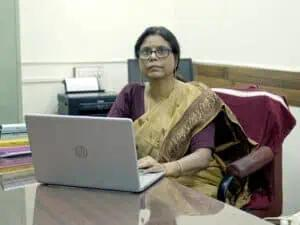
\includegraphics[width=\linewidth]{assets/images/principal_shila_ghosh.jpg}
\end{minipage}
\hfill
\begin{minipage}[c]{0.73\textwidth}
  {\large\bfseries Prof. (Dr.) Shila Ghosh\par}
  \smallskip
  {\itshape Professor \& Principal\par}
\end{minipage}

\vspace{0.7cm}
{\justifying
It gives me immense pleasure to share a few words on the publication of Volume X of \textit{Electronic Trends}, the Departmental Technical Magazine of Electronics \& Communication Engineering. This magazine reflects the curiosity, creativity, and enthusiasm of our students and faculty members, while also highlighting the department's continued commitment to technical excellence, research, innovation, and all-round development.

\medskip
Every edition provides an opportunity to celebrate the ideas, achievements, and collaborative efforts that strengthen our academic community. Volume X carries this tradition forward through thoughtful technical articles, emerging-technology discussions, student contributions, project insights, and glimpses of the academic and co-curricular activities undertaken during the year.

\medskip
I sincerely appreciate the editorial board, faculty coordinators, contributors, and student volunteers whose dedication has shaped this edition. Bringing together a publication of this nature requires patience, teamwork, and careful attention to detail. Their efforts have made the magazine both informative and engaging and reflect the values of responsibility and continuous improvement upheld by our institution.

\medskip
I encourage our students to use this platform to express original ideas, share their learning, and develop the confidence to explore beyond the classroom. In a rapidly changing technological world, the willingness to question, experiment, collaborate, and continue learning is as important as technical knowledge itself. I hope this volume inspires its readers to pursue meaningful innovation and approach future challenges with integrity and purpose.

\medskip
I extend my warm congratulations to everyone associated with Volume X and wish the Department of Electronics \& Communication Engineering continued progress and success in all its future endeavours.\par}

\medskip
\begin{flushright}
  \textbf{Prof. (Dr.) Shila Ghosh}\par
  Principal\par
  {\small St. Thomas' College of Engineering \& Technology, Kolkata\par}
\end{flushright}

\vfill\null

\thispagestyle{fancy}

\begin{center}
  {\LARGE\bfseries Message from the Dean (Academic)\par}
\end{center}

\vspace{0.7cm}
\noindent
\begin{minipage}[c]{0.18\textwidth}
  \centering
  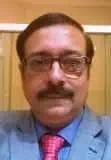
\includegraphics[height=4cm]{assets/images/dean_sujit_biswas.jpg}
\end{minipage}
\hfill
\begin{minipage}[c]{0.77\textwidth}
  {\large\bfseries Prof. (Dr.) Sujit Kumar Biswas\par}
  \smallskip
  {\itshape Professor \& Dean (Academic)\par}
\end{minipage}

\vspace{0.7cm}
{\justifying
It gives me immense pleasure to extend my greetings and best wishes to the Department of Electronics \& Communication Engineering on the publication of Volume X of the Departmental Technical Magazine, \textit{Electronic Trends}. This annual magazine stands as a reflection of the department's dedication to academic excellence, research, innovation, and the holistic development of its students and faculty members.

\medskip
In today's rapidly advancing technological era, it is essential for students to nurture curiosity, explore emerging technologies, and actively engage in continuous learning. This edition presents a diverse collection of technical articles, project insights, achievements, and creative contributions that highlight the talent, commitment, and enthusiasm of our students and faculty members.

\medskip
The consistent efforts of the department to foster a dynamic academic environment, encourage interdisciplinary collaboration, and promote participation in technical and professional activities are truly commendable. This magazine reflects the collective commitment of the department toward delivering quality education and research excellence.

\medskip
I congratulate the editorial board, faculty coordinators, and contributors for their dedication and teamwork in bringing out this well-organized publication. I am confident that Volume X will inspire students to aim higher, embrace innovation, and contribute meaningfully to the technological world.

\medskip
My best wishes to the department for its continued growth and accomplishments.\par}

\medskip
\begin{flushright}
  \textbf{Prof. (Dr.) Sujit Kumar Biswas}\par
  Professor \& Dean\par
  {\small St. Thomas' College of Engineering \& Technology, Kolkata\par}
\end{flushright}

\vfill\null

\thispagestyle{fancy}

\begin{center}
  {\LARGE\bfseries Message from the Head\par}
\end{center}

\vspace{0.7cm}
\noindent
\begin{minipage}[c]{0.23\textwidth}
  \centering
  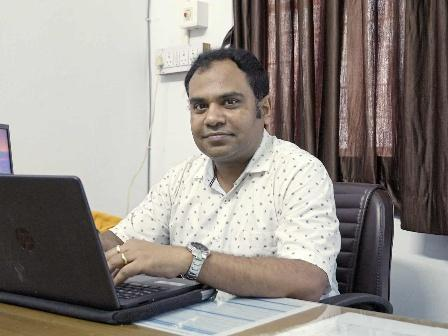
\includegraphics[width=\linewidth]{assets/images/head_prasun_chowdhury.jpg}
\end{minipage}
\hfill
\begin{minipage}[c]{0.72\textwidth}
  {\large\bfseries Dr. Prasun Chowdhury\par}
  \smallskip
  {\itshape Associate Professor \& Head\par}
\end{minipage}

\vspace{0.7cm}
{\justifying
I am delighted to present Volume X of our Departmental Technical Magazine, \textit{Electronic Trends}, a platform that continues to capture the academic excellence, technical curiosity, and creative strengths of our students and faculty members. This edition reflects the steady progress of the department and our commitment to fostering a dynamic learning environment rooted in innovation, research, and collaborative growth.

\medskip
Over the past year, our department has achieved significant milestones---through student projects, research publications, technical workshops, industry interactions, and various academic initiatives that have enriched the overall learning experience. The contributions featured in this volume highlight the dedication, capability, and perseverance of our academic community.

\medskip
This magazine is more than a collection of technical articles; it is a celebration of ideas, exploration, and continuous development. I sincerely appreciate the efforts of the editorial board, faculty coordinators, and student volunteers who have worked diligently to bring out this edition with professionalism and excellence.

\medskip
I encourage all students to actively participate in technical endeavours, stay updated with emerging technologies, and develop the skills necessary to thrive in a rapidly evolving global environment. I am confident that this publication will inspire many to think innovatively, pursue research with passion, and strive for excellence in all their pursuits.

\medskip
My best wishes to everyone involved in making Volume X a meaningful and successful publication.\par}

\medskip
\begin{flushright}
  \textbf{Dr. Prasun Chowdhury}\par
  Associate Professor \& Head\par
  Electronics \& Communication Engineering\par
  {\small St. Thomas' College of Engineering \& Technology, Kolkata\par}
\end{flushright}

\vfill\null

\thispagestyle{fancy}

\begin{center}
  {\LARGE\bfseries Message from the Editorial Board\par}
\end{center}

\vspace{1.1cm}
{\small\justifying
It is our pleasure to present Volume X of our Departmental Technical Magazine, \textit{Electronic Trends}. Every page of this edition reflects the curiosity, creativity, and hard work of the students and faculty members of the Electronics \& Communication Engineering Department. More than a record of the year, the magazine is a shared space where technical knowledge, fresh ideas, and individual experiences come together.

\medskip
While preparing this volume, we wanted to create something that readers could both learn from and enjoy. The articles, project discussions, emerging-technology features, departmental events, and creative sections included here reveal the many ways in which our academic community continues to explore, experiment, and grow. Each contribution brings a distinct perspective and gives this volume its character.

\medskip
The making of Volume X has itself been a valuable learning experience. It brought together different batches, interests, and areas of expertise, reminding us that engineering grows strongest when knowledge is shared openly. Conversations with authors, careful rounds of editing, the selection of photographs, and the organisation of each page taught us that a magazine is shaped as much by cooperation and attention to detail as it is by the ideas it contains.

\medskip
We are sincerely grateful to our Principal, Dean, Head of the Department, faculty members, and student contributors for their guidance, encouragement, and trust throughout the preparation of this magazine. We also thank every member of the editorial team and each volunteer who helped collect, review, organise, and refine the material. Their patience and teamwork transformed a collection of submissions into a complete publication.

\medskip
We hope Volume X encourages readers to remain curious, question familiar ideas, and engage confidently with the rapidly changing world of electronics and communication. At a time when technology is reshaping everyday life, we believe students must not only understand new systems but also consider how those systems can be designed responsibly, inclusively, and for the benefit of society.

\medskip
If this edition inspires even one reader to investigate a new concept, begin a project, or share an original idea, it will have fulfilled its purpose. We invite you to read, reflect, and celebrate the people and possibilities represented in these pages. May this volume become both a record of our present efforts and an encouragement for the students who will shape future editions of \textit{Electronic Trends}.\par}

\medskip
\begin{flushright}
  Warm regards,\par
  \textbf{Editorial Board}\par
  \textbf{Electronic Trends}\par
\end{flushright}

\vfill\null

\begin{center}
  \section*{Vision of \\ St. Thomas' College of Engineering \& Technology}
\end{center}

\justify
To evolve as an industry oriented, research based Institution with ethical values for creative solutions in various engineering domains, with an ultimate objective of meeting technological challenges faced by the Nation and the Society.

\begin{center}
  \section*{Mission of \\ St. Thomas' College of Engineering \& Technology}
\end{center}

\begin{itemize}
  \item \textbf{M1:} To enhance the quality of engineering education and delivery through accessible, comprehensive and research oriented teaching-learning-assessment processes in the state-of-art environment.
  \item \textbf{M2:} To create opportunities for students and faculty members to acquire professional knowledge with multidisciplinary approach and develop managerial, entrepreneurial and social attitudes with highly ethical and moral values.
  \item \textbf{M3:} To satisfy the ever-changing needs of the nation with respect to evolution and absorption of sustainable and environment friendly technologies for effective creation of knowledge-based society in the global era.
\end{itemize}

\noindent
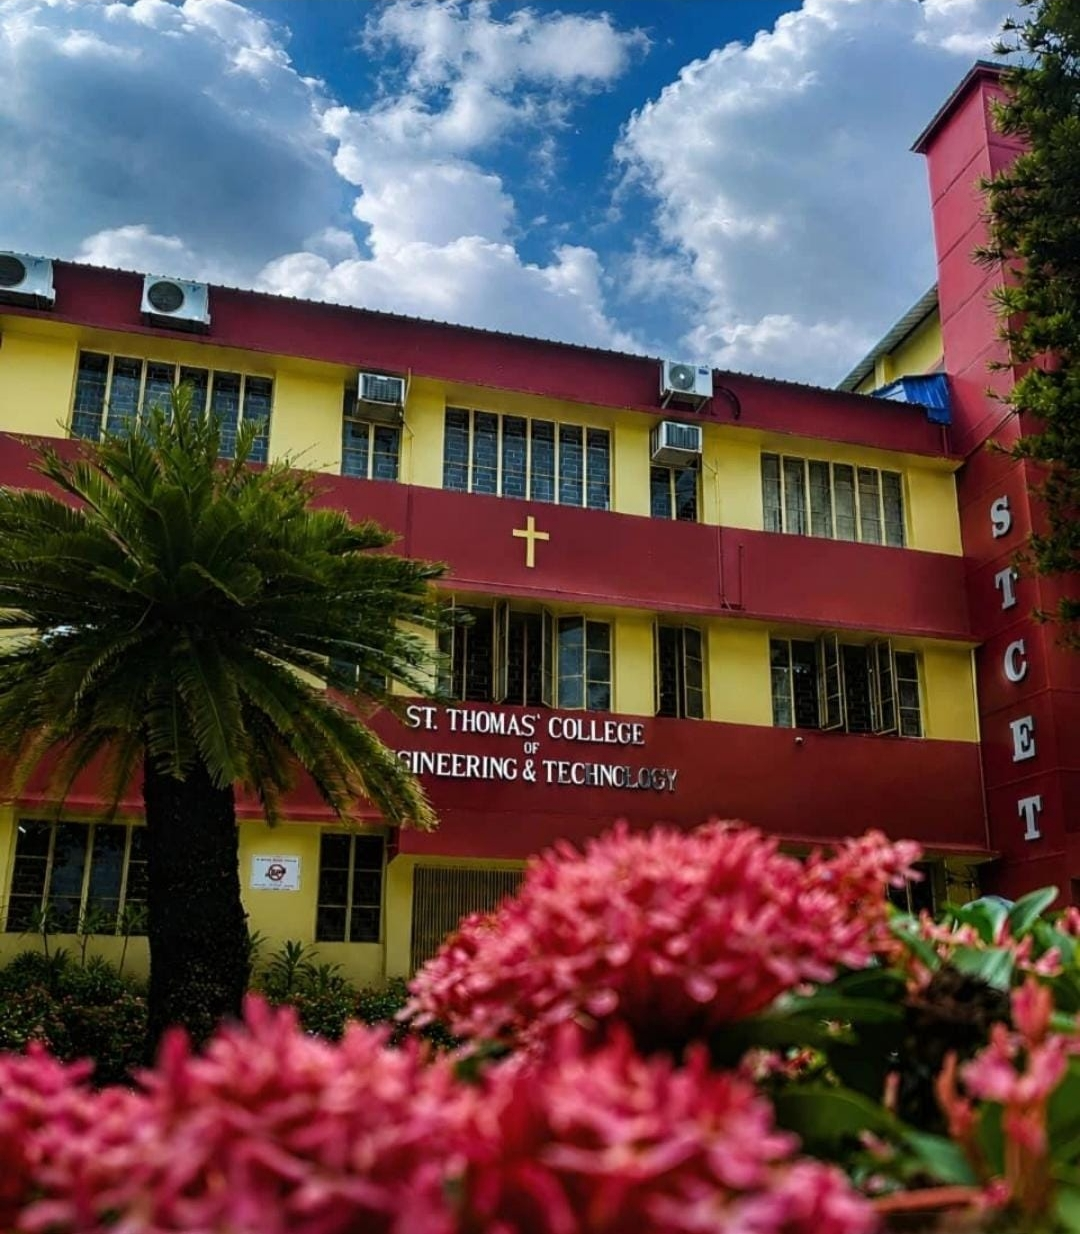
\includegraphics[width=0.5\textwidth, height=8cm]{assets/images/college-pic-3.jpeg}%
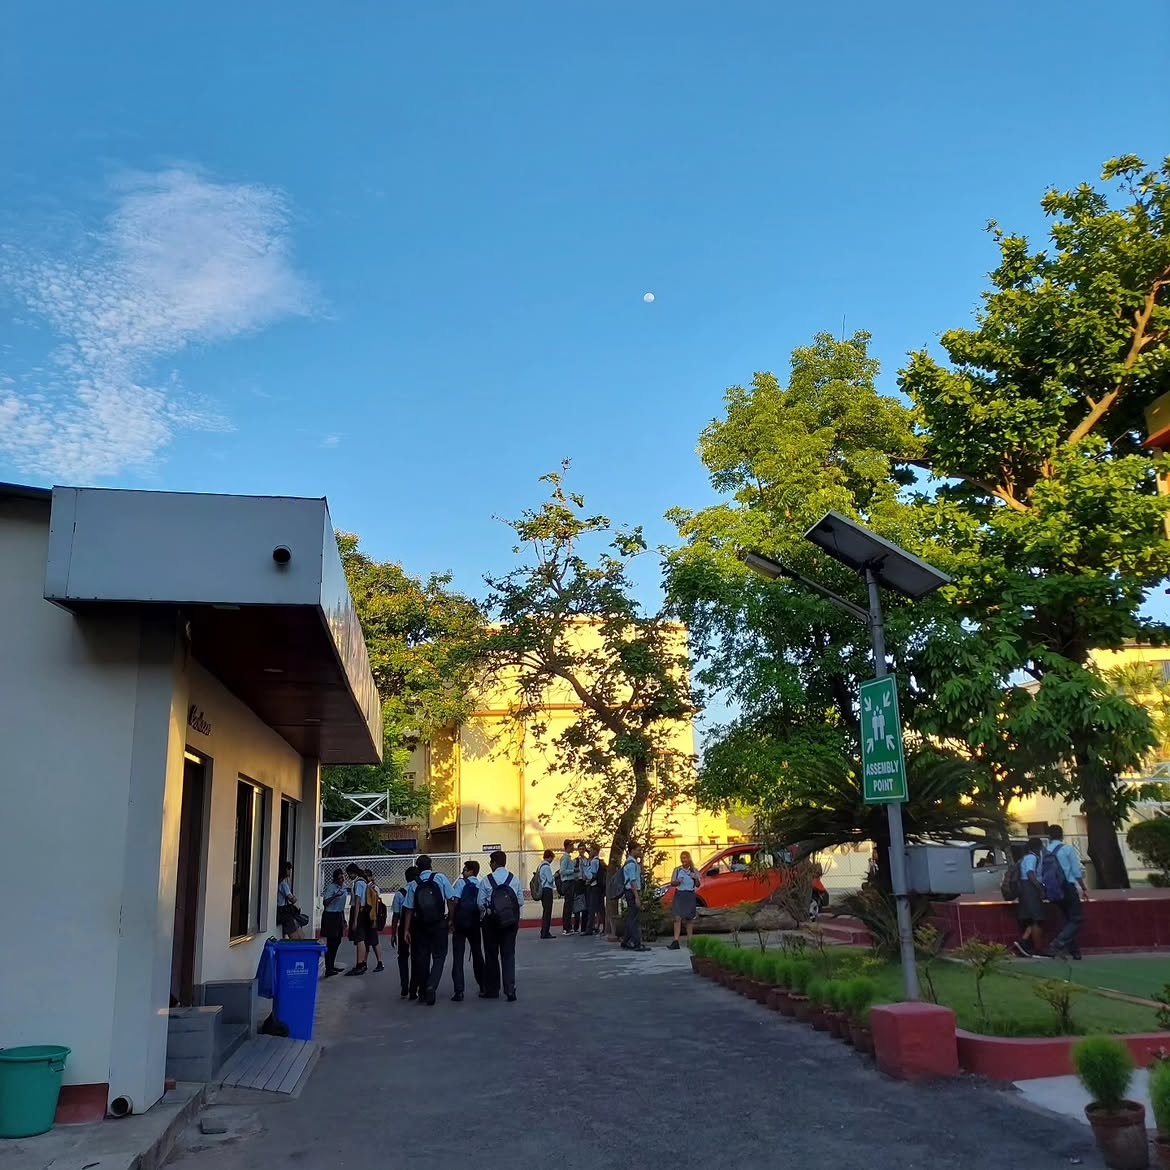
\includegraphics[width=0.5\textwidth, height=8cm]{assets/images/college-pic-2.jpeg}
\newpage
\begin{center}
  \section*{Vision of \\Electronics \& Communication Engineering Department}
\end{center}

\justify
To foster excellence in teaching and research to converge multidisciplinary approach, and sustainability with ethical values for evolving industrial and academic needs in Electronics and Communication Engineering.

\begin{center}
  \section*{Mission of \\Electronics \& Communication Engineering Department}
\end{center}

\begin{itemize}
  \item \textbf{M1:} To produce industry-ready Electronics and Communication professionals through innovative, lab-based and project-driven education in a modern environment.
  \item \textbf{M2:} To advance research in Electronics and Communication Engineering for the competitive and sustainable development of the country.
  \item \textbf{M3:} To develop the department as a learning center for advancing Electronics and Communication Engineering with social values, environmental awareness and entrepreneurial mindset.
\end{itemize}

\noindent
\begin{minipage}[t]{0.5\textwidth}
  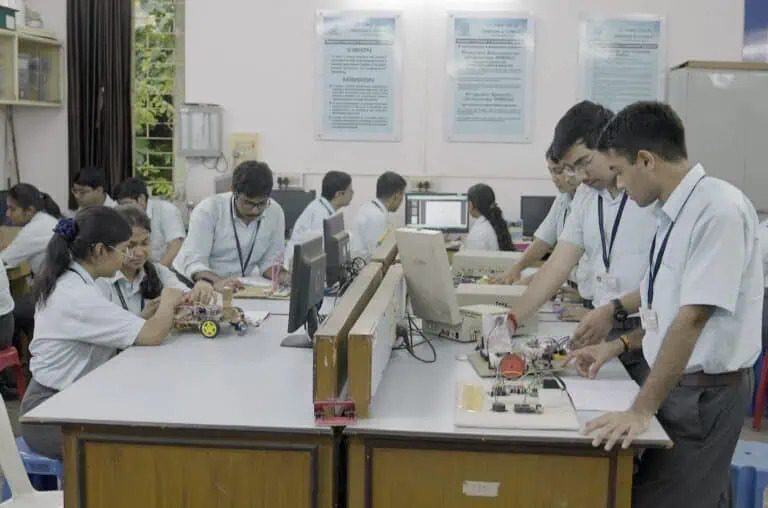
\includegraphics[width=\linewidth, height=6cm]{assets/images/ece-1.jpg}
\end{minipage}%
\begin{minipage}[t]{0.5\textwidth}
  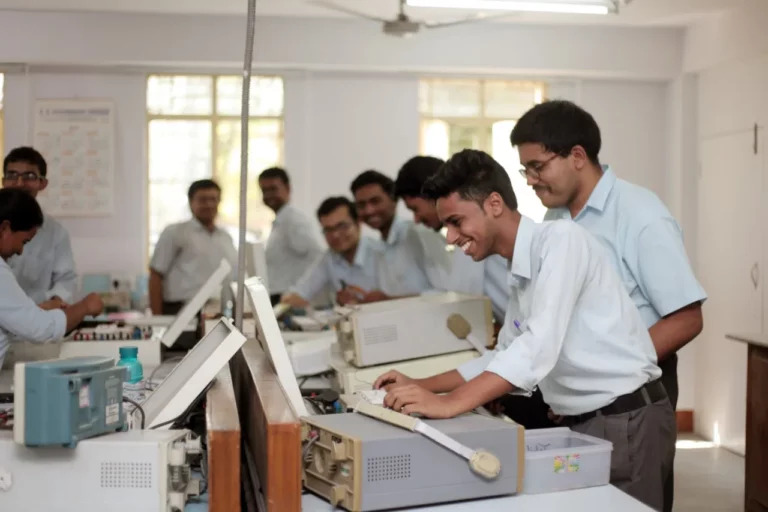
\includegraphics[width=\linewidth, height=6cm]{assets/images/ece-3.jpg}
\end{minipage}

\newpage
\begin{center}
  \section*{Program Educational Objectives (PEOs)}
\end{center}
\justify
Graduates of the Electronics and Communication Engineering program shall:
\begin{itemize}
  \item \textbf{PEO1:} Possess design skills and core proficiency in Electronics \& Communication Engineering for employment in relevant industries.
  \item \textbf{PEO2:} Possess strong core and advanced knowledge in Electronics \& Communication Engineering to pursue higher studies.
  \item \textbf{PEO3:} Exhibit leadership, ethical values, and social commitment to contribute in academia, industry and/or entrepreneurial ventures, both nationally and globally.
\end{itemize}

\begin{center}
  \section*{Program Specific Outcomes (PSOs)}
\end{center}
\justify
After completion of the program, a graduate engineer would have an ability to:
\begin{itemize}
  \item \textbf{PSO1. Professional skills:} Solve real life problems relevant to Electronics and Communication Engineering in various areas, like VLSI, Nano-technology, Advanced Communications, Signal Processing, Embedded Systems, IoT and applications involving AI \& ML.
  \item \textbf{PSO2. Competency:} Demonstrate competence in qualifying exams and pursue successful careers in employment, research and higher education at state, national, and international levels.
\end{itemize}

\begin{figure}[h]
  \centering
  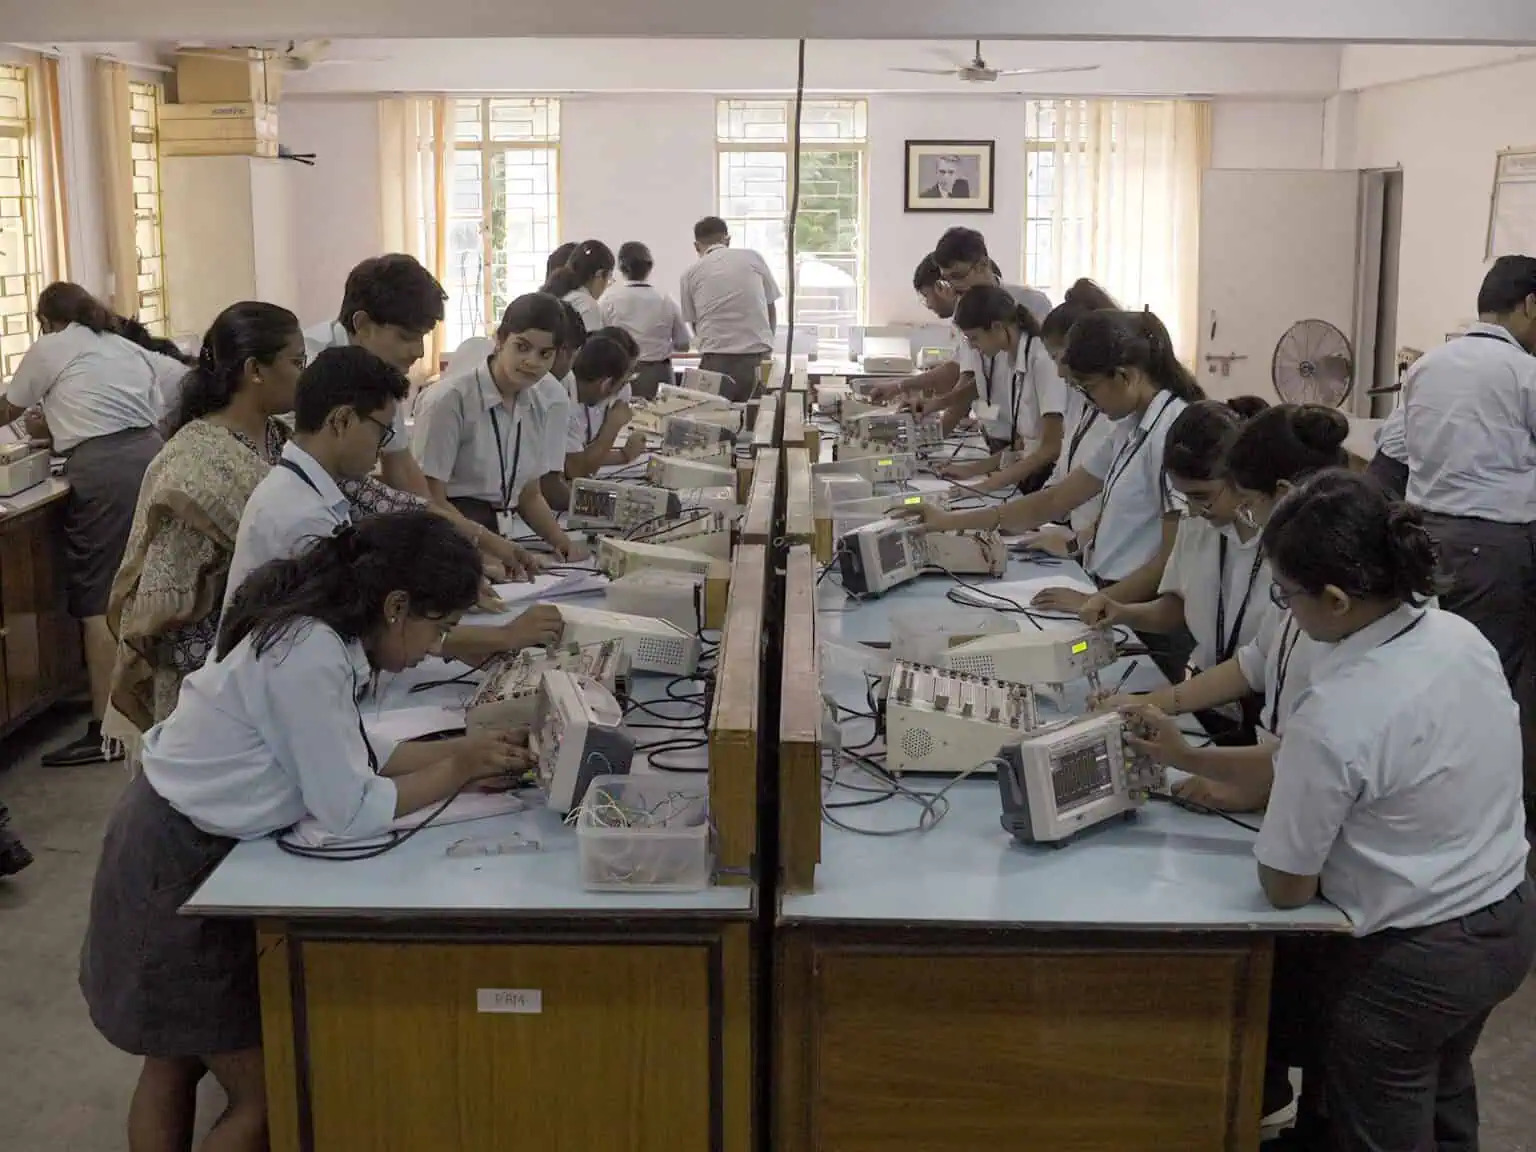
\includegraphics[width=\textwidth, keepaspectratio]{assets/images/ece-2.jpg}
\end{figure}

\newpage

\begin{center}
  \section*{About the Department of Electronics \& Communication Engineering}
\end{center}

\justify
The Department of Electronics and Communication Engineering (ECE) at St. Thomas College of Engineering \& Technology represents the pinnacle of technical education, delivering a comprehensive curriculum that seamlessly integrates core electronics principles with emerging technologies. Our program emphasizes mastery of analog and digital circuit design, electromagnetic theory, communication systems, and microprocessor architecture, preparing students for the full spectrum of ECE career paths.

\vspace{0.5em}

State-of-the-art laboratories equipped with cutting-edge instrumentation—including network analyzers, logic analyzers, high-frequency oscilloscopes, and advanced PCB design workstations—enable practical implementation of complex systems. Specialized facilities support research in RF/microwave engineering, embedded systems development, VLSI prototyping, and digital signal processing applications critical to modern telecommunications infrastructure.

\vspace{0.5em}

\justify
Faculty expertise spans semiconductor device physics, antenna design, wireless protocol development, and machine learning applications in signal processing, supported by ongoing research funded through national grants and industry partnerships. Our graduates excel in core technical roles across semiconductor fabrication, telecommunications infrastructure, embedded systems design, and defense electronics, consistently securing positions with leading organizations in India's rapidly expanding electronics sector.

\begin{figure}[h]
  \centering
  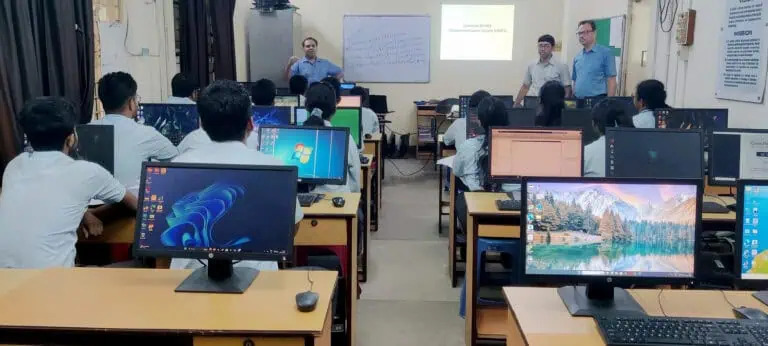
\includegraphics[width=\textwidth, keepaspectratio]{assets/images/ece-4.jpg}
\end{figure}

\newpage

\thispagestyle{empty}

\vspace*{\fill}

\begin{center}
  {\color{IEEEorange}\rule{0.18\textwidth}{1.5pt}}\par
  \vspace{1.2em}

  \begin{minipage}{0.82\textwidth}
    \centering
    
\begin{tikzpicture}
      \node[
        inner sep=0pt,
        align=center,
        transform shape,
        xslant=0.12
      ] {
        {\normalfont\cursive\fontsize{21}{31}\selectfont ``A computer would deserve}\\[0.12em]
        {\normalfont\cursive\fontsize{21}{31}\selectfont to be called intelligent}\\[0.12em]
        {\normalfont\cursive\fontsize{21}{31}\selectfont if it could deceive a human}\\[0.12em]
        {\normalfont\cursive\fontsize{21}{31}\selectfont into believing that it was human.''}};
    \end{tikzpicture}\par

    \vspace{1.5em}
    {\rmfamily\Large\itshape\color{IEEEblue}--- Alan Turing\par}
  \end{minipage}

  \vspace{1.2em}
  {\color{IEEEorange}\rule{0.18\textwidth}{1.5pt}}\par
\end{center}

\vspace*{\fill}

\newpage

\customtableofcontents



\thispagestyle{empty}
\vspace*{\fill}
\addcontentsline{toc}{section}{Reports}
\begin{center}
    \section*{\normalfont\fontsize{60}{72}\selectfont\cursive Reports}
\end{center}
\vspace*{\fill}

\newpage

\pagenumbering{arabic}

\begin{center}
  \section{\capitalisewords{Next-Generation Networking and Communication Protocols for IoT}}
  Dr. Prasun Chowdhury, Associate Professor, ECE
\end{center}

\setcounter{figure}{0}
\setcounter{table}{0}

\begingroup
  \setlength{\parskip}{1pt}
  \setlength{\multicolsep}{3pt}
  \setlength{\abovecaptionskip}{1.5pt}
  \setlength{\belowcaptionskip}{1.5pt}

\begin{multicols}{2}

  \begin{abstract}
    \bfseries
    The Internet of Things (IoT) connects sensors, actuators, embedded processors, gateways, cloud platforms, and intelligent applications into large-scale cyber-physical systems. Its success depends on networking technologies that can accommodate constrained hardware, limited energy, intermittent links, heterogeneous protocols, mobility, and strong security requirements. This article reviews the evolution of IoT networking, layered architectures, device communication models, protocol stacks, short- and long-range connectivity, application protocols, Quality of Service (QoS), interoperability, edge and cloud computing, Industrial IoT, and emerging paradigms such as 6G, artificial-intelligence-assisted networking, blockchain, and satellite IoT. The discussion shows that no single protocol is ideal for every deployment: engineers must balance range, data rate, latency, power, reliability, scalability, cost, and security according to the application.
  \end{abstract}

  \subsection*{\centering\uppercase{Introduction}}
  IoT transforms physical objects into networked information sources and control points. Sensors observe temperature, pressure, vibration, location, motion, or biomedical variables; processors interpret those measurements; communication modules exchange data; and actuators modify the physical environment. The resulting systems support healthcare, agriculture, smart cities, transportation, industrial automation, environmental monitoring, and home automation.

  \noindent
  Networking is the element that turns isolated embedded devices into a coordinated system. It enables addressing, routing, data transfer, remote supervision, firmware updates, service discovery, and automated decisions. A traffic sensor, for example, becomes operationally useful only when its observations can reach a controller or edge platform that adjusts signals and shares information with other services.

  \subsection*{\centering\uppercase{Evolution of IoT Networking}}
  Early embedded systems were designed for a single local function and had little memory, processing power, or connectivity. Interfaces such as RS-232, I$^2$C, SPI, and CAN later allowed nearby components to exchange data. Ethernet extended communication across wired networks, while wireless sensor networks introduced battery-powered nodes capable of multi-hop sensing and forwarding.

  \noindent
  The integration of Internet connectivity, low-cost microcontrollers, Wi-Fi, Bluetooth Low Energy (BLE), cloud services, and mobile applications produced today's smart objects. IPv6 is especially important because its 128-bit address space can identify vastly more devices than IPv4. Adaptation mechanisms such as 6LoWPAN allow IPv6 packets to operate over constrained IEEE 802.15.4 networks with reduced header overhead [1, 2].

  \subsection*{\centering\uppercase{Layered IoT Architecture}}
  A three-layer model divides an IoT system into perception, network, and application layers. The perception layer contains sensors and actuators; the network layer transfers and routes data; and the application layer provides domain-specific services and user interfaces.

  \noindent
  More detailed models add transport, processing, and middleware functions. Processing may occur at an edge node or cloud platform, while middleware manages devices, data formats, APIs, discovery, and access control. Layering improves modularity, but security and management must span the complete system rather than remain confined to one layer.

  \begin{center}
\vspace{-0.9em}
\begin{minipage}{0.98\columnwidth}
\centering
    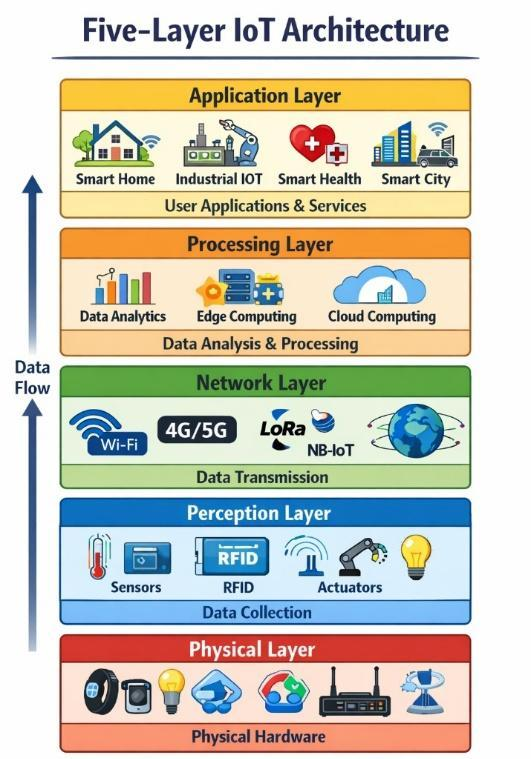
\includegraphics[width=0.50\columnwidth]{assets/images/faculty_pc_five_layer.jpg}
    \captionof{figure}{A layered view of IoT sensing, networking, processing, and applications.}
\end{minipage}
  \end{center}
\vspace{-0.9em}

  \subsection*{\centering\uppercase{Communication Models}}
  IoT devices exchange information through four common models:
  \begin{itemize}\justifying
    \item \textbf{Device-to-device:} nearby devices communicate directly through BLE, Zigbee, NFC, or another local link. This reduces latency and avoids dependence on a remote server.
    \item \textbf{Device-to-gateway:} a gateway aggregates data, translates protocols, enforces security, and forwards selected information to other networks or the cloud.
    \item \textbf{Device-to-cloud:} a device connects directly to an Internet service through Wi-Fi or cellular connectivity, simplifying central analytics and remote access.
    \item \textbf{Back-end data sharing:} authorised applications access common platform data through APIs, enabling cross-domain analytics and service integration.
  \end{itemize}

  \subsection*{\centering\uppercase{The IoT Protocol Stack}}
  IoT communication follows a layered stack adapted to devices with limited memory, power, and packet size. The physical layer defines modulation, spectrum, and signal transmission. The data-link layer controls framing, channel access, link addressing, and error detection. Technologies include Ethernet, Wi-Fi, BLE, IEEE 802.15.4, and LoRa.

  \noindent
  At the network layer, IPv6 provides addressing, 6LoWPAN compresses and fragments IPv6 packets for constrained links, and the Routing Protocol for Low-Power and Lossy Networks (RPL) supports multi-hop routing [1--3]. TCP offers reliable connection-oriented transport, whereas UDP reduces overhead and is often paired with lightweight application protocols. TLS protects TCP sessions, while DTLS provides comparable protection for datagram communication.

  \begin{center}
\vspace{-0.9em}
\begin{minipage}{0.98\columnwidth}
\centering
    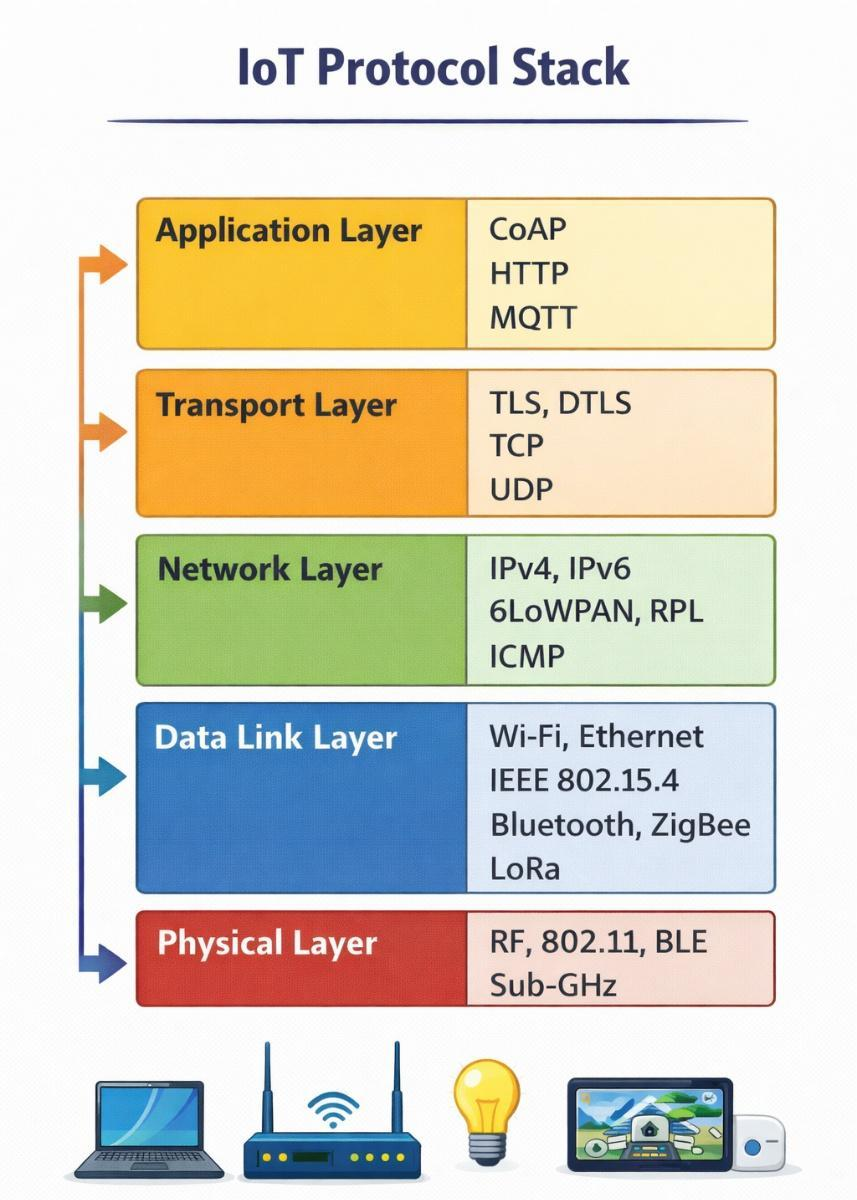
\includegraphics[width=0.70\columnwidth]{assets/images/faculty_pc_protocol_stack.jpg}
    \captionof{figure}{Protocols and technologies across a representative IoT stack.}
\end{minipage}
  \end{center}
\vspace{-0.9em}

  \needspace{4\baselineskip}
  \subsection*{\centering\uppercase{Short-Range Connectivity}}
  BLE operates in the 2.4-GHz band and is designed for small data exchanges with long battery life. It is widely used in wearables, beacons, fitness devices, and health monitors. Zigbee builds low-data-rate mesh networks over IEEE 802.15.4, allowing messages to pass through intermediate nodes. Z-Wave uses sub-GHz spectrum in home-automation networks, reducing interference from crowded 2.4-GHz systems.

  \noindent
  The choice among these technologies depends on topology, payload size, battery target, commissioning method, interoperability, security, and the availability of a gateway. A mesh extends coverage but increases routing and maintenance complexity.

  \subsection*{\centering\uppercase{Wide-Area Connectivity}}
  Wi-Fi offers relatively high throughput within homes, campuses, and industrial sites but normally consumes more power than constrained-radio solutions. Cellular systems provide managed infrastructure, mobility, and broad coverage. NB-IoT targets low-throughput devices requiring deep coverage and long battery life, while LTE-M supports higher rates and mobility.

  \noindent
  Low-Power Wide-Area Network (LPWAN) technologies such as LoRaWAN connect distant sensors that send small payloads infrequently. They are effective for soil monitoring, utility metering, and logistics, but are not designed for video or continuous low-latency control. Engineers must account for duty-cycle limits, link budget, gateway density, spectrum rules, and downlink capacity.

\end{multicols}

\begin{table}[!b]
\noindent\hfill\begin{minipage}{0.48\textwidth}
\raggedright
Table~1 summarizes representative IoT communication technologies and their design trade-offs.\par
\end{minipage}\par
\centering
\caption{Representative IoT communication technologies and design trade-offs.}
\normalsize
  \setlength{\tabcolsep}{2.5pt}
  \renewcommand{\arraystretch}{1.8}
  \begin{tabular}{@{}>{\bfseries\RaggedRight\arraybackslash}p{0.16\textwidth}
                      >{\Centering\arraybackslash}p{0.14\textwidth}
                      >{\Centering\arraybackslash}p{0.12\textwidth}
                      >{\RaggedRight\arraybackslash}p{0.20\textwidth}
                      >{\RaggedRight\arraybackslash}p{0.25\textwidth}@{}}
    \toprule
    \textbf{Technology} & \textbf{Typical Range} & \textbf{Energy Use} & \textbf{Strength} & \textbf{Representative Use} \\
    \midrule
    BLE & Short & Very low & Phone compatibility and low-power operation & Wearables and medical sensors \\
    Zigbee / IEEE 802.15.4 & Short to multi-hop & Low & Mesh networking and many local nodes & Smart lighting and building control \\
    Wi-Fi & Local-area & Moderate to high & High throughput and direct IP connectivity & Cameras, appliances, and gateways \\
    LoRaWAN & Long & Very low & Long range with small, infrequent payloads & Agriculture and environmental sensing \\
    NB-IoT / LTE-M & Wide-area & Low to moderate & Managed cellular coverage and mobility & Metering, logistics, and asset tracking \\
    5G & Wide-area & Varies & High capacity, mobility, and low-latency services & Vehicles, automation, and massive IoT \\
    \bottomrule
  \end{tabular}
\end{table}
\newpage

\noindent\begin{minipage}{\textwidth}
\centering
\captionof{table}{Comparison of common IoT application protocols.}
\scriptsize
  \setlength{\tabcolsep}{2.5pt}
  \renewcommand{\arraystretch}{1.12}
  \begin{tabular}{@{}>{\bfseries\RaggedRight\arraybackslash}p{0.16\textwidth}
                      >{\RaggedRight\arraybackslash}p{0.18\textwidth}
                      >{\Centering\arraybackslash}p{0.11\textwidth}
                      >{\RaggedRight\arraybackslash}p{0.20\textwidth}
                      >{\RaggedRight\arraybackslash}p{0.22\textwidth}@{}}
    \toprule
    \textbf{Protocol} & \textbf{Communication Pattern} & \textbf{Transport} & \textbf{Main Advantage} & \textbf{Typical Placement} \\
    \midrule
    MQTT & Publish--subscribe through a broker & TCP & Lightweight telemetry with selectable delivery QoS & Sensors, gateways, and cloud brokers \\
    CoAP & REST request--response and observation & UDP & Compact headers and constrained-device support & Local constrained IP networks \\
    HTTP/HTTPS & REST request--response & TCP & Universal web and cloud compatibility & Gateways, dashboards, and cloud APIs \\
    AMQP & Queues, routing, and publish--subscribe & TCP & Reliable enterprise messaging & Back-end and industrial integration \\
    \bottomrule
  \end{tabular}
\end{minipage}
\par\vspace{4pt}
\noindent\begin{minipage}{0.48\textwidth}
\raggedright
Table~2 compares common IoT application protocols and their typical placements.\par
\end{minipage}
\par\vspace{4pt}

\begin{multicols}{2}

  \subsection*{\centering\uppercase{Application-Layer Protocols}}
  \subsubsection*{MQTT}
  MQTT uses a publish--subscribe model. Devices publish messages to named topics through a broker, and subscribers receive topics of interest. This decouples producers and consumers and supports scalable telemetry. MQTT defines QoS 0 (at most once), QoS 1 (at least once), and QoS 2 (exactly once), trading overhead for delivery assurance [4].

  \subsubsection*{CoAP}
  The Constrained Application Protocol (CoAP) follows a REST-style request--response model similar to HTTP but normally uses UDP. Compact binary headers, multicast support, resource observation, and DTLS or object security make it suitable for constrained nodes [5].

  \subsubsection*{HTTP and AMQP}
  HTTP/HTTPS remains common between gateways, web applications, and cloud platforms because tools and services support it universally. Its overhead may be excessive for very constrained endpoints. AMQP provides reliable message queuing and routing for enterprise and industrial integration where richer broker functionality is required.

  \subsection*{\centering\uppercase{Quality of Service}}
  IoT performance is measured through latency, jitter, throughput, packet loss, reliability, and availability. Requirements vary sharply: a soil sensor may tolerate minutes of delay, while a protection relay or robotic controller may require deterministic response. QoS must therefore be designed across the radio, scheduling, routing, transport, application, and computing layers.

  \subsection*{\centering\uppercase{Security Across the Stack}}
  {\justifying
    IoT devices often operate unattended, handle sensitive data, and control physical equipment. Major threats include spoofing, replay, malware, tampering, denial-of-service, and insecure firmware; one compromised endpoint can expose a wider network.

    \noindent
    Defence requires unique identities, secure boot and key storage, signed updates, least privilege, and removal of default passwords. AES, ECC, TLS or DTLS, segmentation, monitoring, certificate management, vulnerability disclosure, and long-term update support provide layered protection [6].\par
  }

  \subsection*{\centering\uppercase{Interoperability and Standardisation}}
  Heterogeneous devices must agree on radio interfaces, addressing, message formats, discovery, security, and application semantics. IEEE develops important physical and MAC standards; the IETF specifies Internet protocols; 3GPP standardises cellular systems; the ITU coordinates international telecommunications; and industry alliances define application profiles.

  \noindent
  Protocol compliance alone does not guarantee interoperability. Two devices may use MQTT but publish incompatible topic structures or data units. Common information models, schemas, APIs, testing programmes, and device-management conventions are needed to achieve plug-and-play behaviour.

  \subsection*{\centering\uppercase{Cloud, Edge, and Fog Communication}}
  Cloud platforms provide scalable storage, analytics, visualisation, fleet management, and integration with business systems. Sending every sample to a distant cloud, however, can increase latency, bandwidth cost, and privacy exposure.

  \noindent
  Edge computing places processing near sensors. A gateway can filter noise, aggregate samples, detect anomalies, and execute urgent control even when the Internet connection is unavailable. Fog architectures distribute these functions across several intermediate nodes. Practical designs divide work according to urgency, computation, energy, privacy, and the value of retaining raw data.

  \begin{center}
\vspace{-0.9em}
\begin{minipage}{0.98\columnwidth}
\centering
    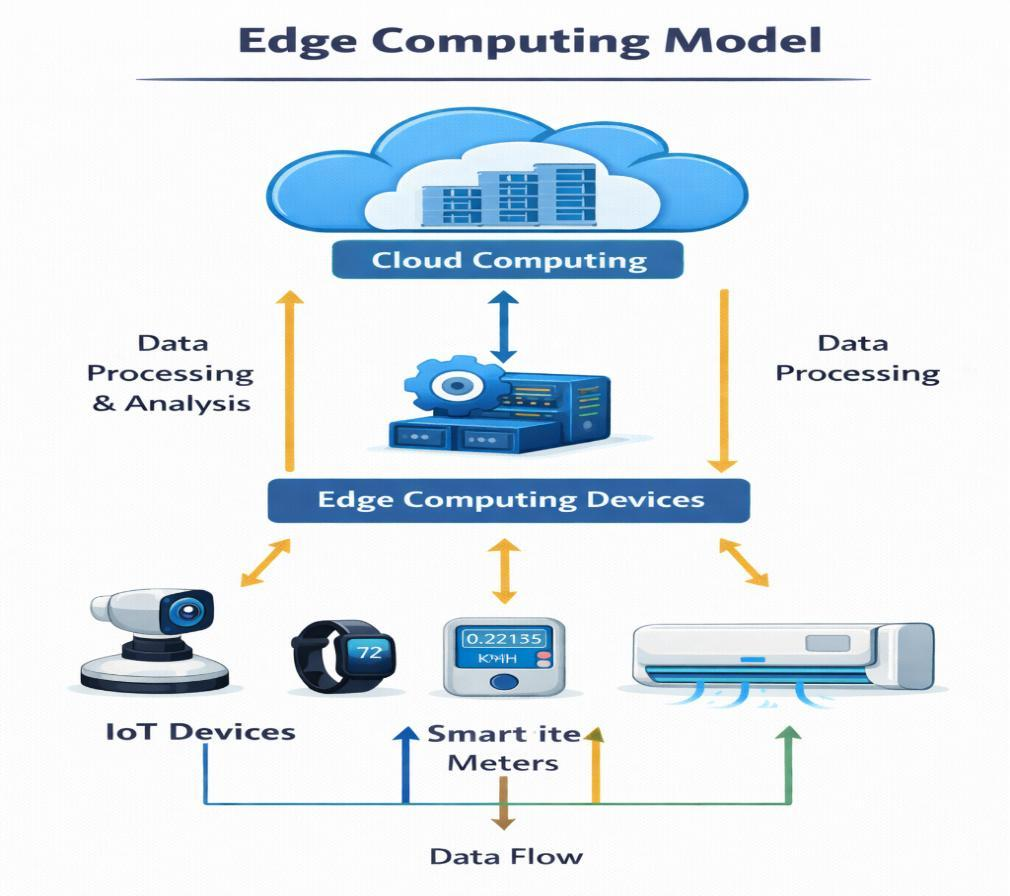
\includegraphics[width=0.75\columnwidth]{assets/images/faculty_pc_edge.jpg}
    \captionof{figure}{Edge nodes process time-sensitive data near IoT devices while coordinating with cloud services.}
\end{minipage}
  \end{center}
\vspace{-0.9em}

  \subsection*{\centering\uppercase{Industrial IoT}}
  Industrial IoT connects machines, robots, instruments, controllers, and supervisory platforms. Representative technologies include Modbus, OPC UA, PROFINET, and EtherCAT. Unlike consumer telemetry, industrial communication may demand bounded latency, deterministic scheduling, high availability, functional safety, and operation alongside legacy equipment.

  \noindent
  Predictive maintenance illustrates the value of IIoT: vibration and temperature sensors feed edge analytics that identify abnormal behaviour before a machine fails. The network must preserve time synchronisation, data integrity, and service continuity without allowing remote connectivity to weaken plant security.

  \subsection*{\centering\uppercase{Applications}}
  In smart agriculture, soil and climate sensors communicate through LPWAN to control irrigation and improve resource use. Smart-city systems coordinate traffic signals, parking, lighting, and waste collection. Healthcare devices monitor heart rate, blood pressure, oxygen saturation, and movement, requiring dependable delivery, privacy, and clinical oversight. Similar networking principles support asset tracking, environmental observation, connected vehicles, and intelligent buildings.

  \subsection*{\centering\uppercase{Emerging Paradigms}}
  \begin{itemize}\justifying
    \item \textbf{6G and massive machine communication:} future systems aim to integrate terrestrial, aerial, and satellite networks with extremely dense sensing and context-aware services.
    \item \textbf{AI-assisted networking:} learning systems can predict faults, estimate congestion, optimise routing, allocate spectrum, and detect abnormal traffic.
    \item \textbf{Blockchain and distributed trust:} tamper-evident ledgers may support shared audit trails and decentralised identity, although computation and storage overhead must be justified.
    \item \textbf{Satellite IoT:} low-Earth-orbit connectivity can reach farms, oceans, pipelines, and remote infrastructure outside terrestrial coverage.
    \item \textbf{Energy-aware networking:} wake-up radios, adaptive duty cycles, energy harvesting, and lightweight protocols extend unattended device life.
  \end{itemize}

  \subsection*{\centering\uppercase{Design Challenges}}
  Large deployments face address management, radio coexistence, changing topology, battery replacement, data overload, vendor fragmentation, physical exposure, and long device lifetimes. Scalable management must automate onboarding, configuration, monitoring, credential rotation, firmware updates, and secure retirement. The technically strongest protocol is not necessarily the best choice if it cannot meet cost, energy, coverage, maintenance, or interoperability constraints.

  \subsection*{\centering\uppercase{Conclusion}}
  IoT networking combines embedded design, radio communication, Internet protocols, distributed computing, security, and application engineering. Layered architectures and gateways help integrate heterogeneous devices, while technologies such as BLE, Zigbee, Wi-Fi, LPWAN, cellular IoT, MQTT, CoAP, IPv6, and RPL address different operating conditions.

  \noindent
  Future systems will increasingly combine edge intelligence, cloud-scale coordination, AI-assisted management, advanced cellular networks, and satellite coverage. Reliable IoT design therefore requires deliberate trade-offs among range, rate, latency, energy, reliability, scalability, interoperability, security, and lifecycle support. Communication is not merely a connection between devices; it is the foundation that allows sensing, computation, and action to operate as one intelligent system.

  \subsection*{\centering\uppercase{References}}
  {\small
  \begin{justify}
    \begin{enumerate}[label={\relax[\arabic*]},leftmargin=*,labelsep=0.5em,itemsep=0.20em,parsep=0pt]
      \item J. Hui and P. Thubert, \textit{Compression Format for IPv6 Datagrams over IEEE 802.15.4-Based Networks}, IETF RFC 6282, 2011.
      \item IEEE, \textit{IEEE Standard for Low-Rate Wireless Networks}, IEEE 802.15.4.
      \item T. Winter et al., \textit{RPL: IPv6 Routing Protocol for Low-Power and Lossy Networks}, IETF RFC 6550, 2012.
      \item OASIS, \textit{MQTT Version 5.0}, OASIS Standard, 2019.
      \item Z. Shelby, K. Hartke, and C. Bormann, \textit{The Constrained Application Protocol (CoAP)}, IETF RFC 7252, 2014.
      \item M. Fagan et al., \textit{IoT Device Cybersecurity Capability Core Baseline}, NISTIR 8259A, 2020.
      \item 3GPP, \textit{Cellular System Support for Ultra-Low Complexity and Low Throughput Internet of Things}.
      \item OPC Foundation, \textit{OPC Unified Architecture Specification}.
    \end{enumerate}
  \end{justify}}
\end{multicols}
\endgroup


\begin{center}
\begin{tcolorbox}[colback=SoftBlue, colframe=IEEEblue!70!black, boxrule=0.5pt, arc=0mm, left=3mm, right=3mm, top=2mm, bottom=2mm, width=0.92\textwidth]
\small\RaggedRight \textbf{\color{IEEEblue!75!black}Did you know?} --- At sub-5\,nm quantum tunneling dominates, which is why FinFETs and gate-all-around nanosheets were invented to keep electrons in check.
\end{tcolorbox}
\end{center}

\begin{center}
  \section{\capitalisewords{Nanoelectronics and Artificial Intelligence}}
  Dr. Dipankar Kundu, Associate Professor, ECE
\end{center}

\setcounter{figure}{0}
\setcounter{table}{0}

\begin{multicols}{2}
  \begin{abstract}
    \bfseries
    Nanoelectronics develops devices, materials, and circuits whose critical dimensions lie in the nanometre regime. Continued miniaturisation has enabled faster processors, dense memories, energy-efficient sensors, high-quality displays, flexible electronics, and compact computing systems. Artificial Intelligence (AI) is now accelerating this field by predicting nanomaterial properties, approximating expensive physical simulations, optimising device geometry and circuit layout, detecting fabrication defects, and controlling manufacturing processes. The relationship is reciprocal: nanoelectronics supplies specialised hardware for AI, including non-volatile memories, in-memory computing arrays, and neuromorphic devices that reduce the energy and data-movement cost of conventional processors. This article reviews the benefits and applications of nanoelectronics, the role of emerging materials, AI-assisted design and fabrication, brain-inspired hardware, technical limitations, and future opportunities for integrated nanoelectronic--AI systems.
  \end{abstract}

  \subsection*{\centering\uppercase{Introduction}}
  Modern electronic systems depend on the ability to place enormous numbers of transistors and memory elements within a small area. Reducing device dimensions shortens signal paths, increases functional density, and permits powerful computation in smartphones, medical instruments, vehicles, communication equipment, and cloud infrastructure. Nanoelectronics extends this development beyond simple geometric scaling by introducing new device structures, materials, fabrication methods, and physical operating principles.

  \noindent
  At nanoscale dimensions, quantum confinement, tunnelling, interface effects, variability, and heat dissipation become increasingly important. Designers must therefore consider atomic-scale behaviour rather than treating a transistor as an ideal switch. This complexity makes nanoelectronics a natural application area for AI and machine learning, which can identify relationships in high-dimensional data and rapidly search large design spaces.

  \subsection*{\centering\uppercase{Why Nanoelectronics Matters}}
  \subsubsection*{Lower Energy Use}
  Smaller devices can switch with less stored charge, reducing the energy required for many operations. A simplified expression for dynamic CMOS power is
  \[
    P_{\mathrm{dynamic}}=\alpha C V^2 f,
  \]
  where $\alpha$ is switching activity, $C$ is effective capacitance, $V$ is supply voltage, and $f$ is operating frequency. Lower capacitance and voltage reduce energy, although leakage current and heat density limit the benefit of continued scaling.

  \subsubsection*{Faster Processing}
  Shorter channels and interconnections reduce carrier transit distance and propagation delay. Advanced devices can therefore support high-speed processors and communication circuits. Performance depends not only on transistor speed, however, but also on interconnect resistance, capacitance, memory access, thermal conditions, and architecture.

  \subsubsection*{High-Density Storage}
  Nanoscale memory cells allow large amounts of information to be stored in a compact footprint. Flash memory, magnetic memories, resistive switching devices, and phase-change materials offer different combinations of density, endurance, retention, access time, and energy consumption.

  \subsubsection*{Flexible and Wearable Systems}
  Thin films, nanowires, two-dimensional materials, and printable conductors enable lightweight sensors and circuits on flexible substrates. Applications include bendable displays, smart textiles, medical patches, electronic skin, and unobtrusive health-monitoring devices.

  \subsection*{\centering\uppercase{Core Applications}}
  Nanoelectronics supports several major technology areas:
  \begin{itemize}\justifying
    \item \textbf{Advanced computing:} high-density logic and memory support microprocessors, accelerators, edge devices, and research toward quantum information systems.
    \item \textbf{Displays:} quantum dots and nanoscale emitters improve colour purity, brightness, thickness, and energy efficiency in television and mobile displays.
    \item \textbf{Sensors and wearables:} nanoscale surfaces respond strongly to chemical, biological, mechanical, and optical changes, enabling sensitive compact detectors.
    \item \textbf{Communication systems:} high-frequency transistors, photonic devices, and compact antennas support faster wired and wireless links.
    \item \textbf{Energy systems:} nanostructured electrodes and materials improve batteries, supercapacitors, solar cells, and energy-harvesting devices.
  \end{itemize}

  \subsection*{\centering\uppercase{Beyond Conventional Silicon}}
  Silicon remains the foundation of semiconductor manufacturing, but continued scaling motivates alternative channel, contact, dielectric, and interconnect materials. Graphene offers exceptional carrier mobility and thermal conductivity, although its lack of a natural bandgap complicates ordinary digital switching [3]. Carbon nanotubes can form narrow transistor channels with strong electrostatic control [4]. Two-dimensional semiconductors, nanowires, and high-permittivity dielectrics provide further routes toward low-power and highly scaled devices.

\end{multicols}

\begin{table}[b]
\centering
\caption{Representative nanoelectronic technologies and their engineering value.}
\footnotesize
  \setlength{\tabcolsep}{4pt}
  \renewcommand{\arraystretch}{1.0}
  \begin{tabular}{@{}>{\bfseries\RaggedRight\arraybackslash}p{0.20\textwidth}
                      >{\RaggedRight\arraybackslash}p{0.28\textwidth}
                      >{\RaggedRight\arraybackslash}p{0.44\textwidth}@{}}
    \toprule
    \textbf{Technology} & \textbf{Key Property} & \textbf{Representative Application} \\
    \midrule
    FinFET / gate-all-around FET & Strong gate control over a small channel & Dense low-power logic and advanced processors \\
    Quantum dots & Size-dependent optical and electronic behaviour & Colour-conversion displays, imaging, and photodetectors \\
    Carbon nanotubes & Nanoscale one-dimensional conduction path & Experimental transistors, sensors, and interconnects \\
    Two-dimensional materials & Atomically thin channels and surfaces & Flexible electronics, sensing, and scaled transistors \\
    Resistive and phase-change memory & Non-volatile programmable conductance & Storage, in-memory computing, and artificial synapses \\
    Nanowires and thin films & High surface-to-volume ratio and flexibility & Biomedical sensors, wearable devices, and energy systems \\
  \bottomrule
  \end{tabular}
\end{table}
\vspace{-0.18em}

\begin{multicols}{2}
  A promising material must satisfy more than one laboratory metric. It must be manufacturable over large areas, stable during processing, compatible with contacts and dielectrics, reproducible across devices, and economically integrated into existing production systems.

  \subsection*{\centering\uppercase{AI for Nanoelectronics}}
  Table~1 summarizes representative nanoelectronic technologies and their engineering value.
  AI supports nanoelectronics at several stages, from material discovery to manufacturing and circuit operation. Its principal advantage is the ability to learn useful approximations from experimental or simulated data and then evaluate new candidates much faster than repeated physical trials.

  \subsubsection*{Discovery of Materials}
  Machine-learning models can screen chemical and structural databases to identify candidate conductors, semiconductors, dielectrics, magnetic materials, and catalysts [5]. Input features may include composition, crystal structure, bonding, calculated energy, or previously measured properties. The model ranks promising candidates, while physical theory and laboratory validation determine whether the prediction is reliable.

  \subsubsection*{Predictive Modelling and Simulation}
  Accurate atomistic and quantum-mechanical calculations may require substantial computation. Surrogate models learn the relationship between device geometry, materials, bias, temperature, and output characteristics. Once trained and validated, they can rapidly estimate current, delay, power, reliability, or process sensitivity. These models do not eliminate physics; they provide a faster approximation within the domain represented by their training data.

  \subsubsection*{Device and Circuit Optimisation}
  Nanoelectronic design contains many coupled variables: channel dimensions, doping, contact resistance, dielectric thickness, operating voltage, layout, and thermal constraints. Optimisation algorithms can search these variables for lower leakage, higher speed, improved yield, or a balanced power--performance--area result. AI-assisted electronic-design automation can also place and route dense circuits while reducing congestion and signal interference.

  \subsubsection*{Nanofabrication Control}
  Lithography, deposition, etching, annealing, and nanoparticle assembly are sensitive to process conditions. Machine vision detects pattern defects, while predictive models connect sensor measurements with final device performance. Real-time control can adjust exposure, temperature, gas flow, pressure, or timing to improve uniformity and yield.

  \subsubsection*{Reliability and Predictive Maintenance}
  AI can analyse electrical measurements, microscopy, acoustic data, and equipment logs to identify abnormal process behaviour. Early detection reduces wafer loss and unplanned downtime. At the device level, learning models can estimate degradation caused by bias stress, temperature cycling, electromigration, or repeated memory programming.

  \subsection*{\centering\uppercase{Nanoelectronics for AI}}
  Conventional processors store data in memory and repeatedly move it to separate computing units. This von Neumann organisation is flexible, but data movement consumes considerable time and energy in large AI workloads. Nanoelectronic devices can reduce this bottleneck through specialised accelerators, non-volatile memory, in-memory computation, and neuromorphic architectures.

  \subsubsection*{In-Memory Computing}
  Crossbar arrays of resistive or phase-change devices can store conductance values representing neural-network weights. Applying input voltages allows currents to accumulate according to Kirchhoff's laws, approximating many multiply--accumulate operations in parallel. The approach can be highly efficient, but practical systems must manage device variation, limited precision, noise, endurance, and analogue-to-digital conversion overhead.

\end{multicols}

\begin{table}[b]
\centering
\caption{The reciprocal relationship between AI and nanoelectronics.}
\footnotesize
  \setlength{\tabcolsep}{4pt}
  \renewcommand{\arraystretch}{1.18}
  \begin{tabular}{@{}>{\bfseries\RaggedRight\arraybackslash}p{0.23\textwidth}
                      >{\RaggedRight\arraybackslash}p{0.31\textwidth}
                      >{\RaggedRight\arraybackslash}p{0.38\textwidth}@{}}
    \toprule
    \textbf{Direction} & \textbf{Method} & \textbf{Engineering Benefit} \\
    \midrule
    AI $\rightarrow$ Nanoelectronics & Material-property prediction and candidate screening & Reduces the number of expensive synthesis and characterisation experiments \\
    AI $\rightarrow$ Nanoelectronics & Fast surrogate device models and optimisation & Accelerates design-space exploration for power, speed, area, and reliability \\
    AI $\rightarrow$ Nanoelectronics & Vision-based inspection and process control & Detects defects and improves fabrication precision and yield \\
    Nanoelectronics $\rightarrow$ AI & Non-volatile and in-memory computing devices & Reduces repeated movement of neural-network weights and data \\
    Nanoelectronics $\rightarrow$ AI & Neuromorphic neurons and synapses & Supports event-driven, brain-inspired computation with low energy \\
    Nanoelectronics $\rightarrow$ AI & Compact sensing and edge accelerators & Enables rapid local decisions with lower communication demand \\
    \bottomrule
  \end{tabular}
\end{table}
\vspace{-0.18em}

\begin{multicols}{2}
  \subsubsection*{Neuromorphic Hardware}
  Neuromorphic systems imitate selected organisational principles of biological nervous systems [6]. Electronic neurons communicate through events or spikes, while synaptic devices store adaptable connection strengths. Processing and memory are placed close together, allowing sparse sensory information to be handled with low energy. Applications include robotics, vision, audio processing, medical monitoring, and always-on edge intelligence.

  \subsubsection*{Edge AI}
  Compact nanoelectronic accelerators allow inference to occur near a sensor rather than in a remote cloud. Local processing reduces communication delay, bandwidth, and exposure of private raw data. It is particularly valuable for wearables, autonomous machines, industrial monitoring, and battery-powered systems.

  \subsection*{\centering\uppercase{An Integrated Development Cycle}}
  Table~2 summarizes the reciprocal relationship between AI and nanoelectronics.
  The strongest results emerge when AI and physical engineering are combined in a closed loop:
  \begin{enumerate}\justifying
    \item define the target electrical, mechanical, optical, or thermal properties;
    \item generate candidate materials and device structures through theory, simulation, or prior experiments;
    \item train a model to predict performance and uncertainty;
    \item fabricate the most informative candidates rather than every possible design;
    \item measure real devices and return the results to the model;
    \item refine the design until performance, manufacturability, reliability, and cost targets are satisfied.
  \end{enumerate}
  This approach is often called active learning or design--build--test--learn. Human expertise remains essential for selecting meaningful objectives, recognising invalid assumptions, and confirming that a statistical improvement corresponds to a physically useful device.

  \subsection*{\centering\uppercase{Challenges}}
  \begin{itemize}\justifying
    \item \textbf{Limited data:} nanoscale experiments are expensive, and datasets may be too small or inconsistent for robust learning.
    \item \textbf{Model generalisation:} a model trained on one material system or fabrication tool may fail under different conditions.
    \item \textbf{Interpretability:} engineers need to understand whether a prediction follows valid physical relationships or accidental correlations.
    \item \textbf{Variability:} atomic defects, interfaces, temperature, and process fluctuations create significant device-to-device differences.
    \item \textbf{Thermal management:} higher functional density can concentrate heat even when individual operations use less energy.
    \item \textbf{Manufacturing integration:} promising laboratory devices must be compatible with repeatable, high-yield, large-scale fabrication.
    \item \textbf{Hardware accuracy:} analogue and neuromorphic devices may exhibit noise, drift, limited precision, and endurance constraints.
  \end{itemize}

  \subsection*{\centering\uppercase{Future Scope}}
  Future research will increasingly combine physics-based simulation with machine learning so that predictions respect conservation laws, symmetries, and known device behaviour. Automated laboratories may connect robotic fabrication, high-throughput measurement, and active-learning algorithms to explore materials with limited human intervention.

  \noindent
  At the system level, heterogeneous integration will combine conventional CMOS with memories, sensors, photonic devices, and specialised accelerators. Three-dimensional integration can shorten data paths but intensifies thermal and testing challenges. Neuromorphic and in-memory systems will continue to develop for applications where low energy and local response matter more than universal numerical precision.

  \subsection*{\centering\uppercase{Conclusion}}
  Nanoelectronics has enabled compact, fast, energy-conscious, and data-rich electronic systems. Its importance extends from processors and memories to displays, sensors, flexible devices, healthcare, communication, and energy technologies. Emerging materials such as graphene, carbon nanotubes, nanowires, and two-dimensional semiconductors expand the available design space beyond conventional silicon.

  \noindent
  AI accelerates this field through material discovery, surrogate simulation, circuit optimisation, defect inspection, fabrication control, and reliability prediction. In return, nanoelectronics provides in-memory and neuromorphic hardware capable of running AI with reduced energy and latency. Their convergence is therefore not a one-way application of software to devices; it is a co-design process in which materials, devices, circuits, architectures, algorithms, and manufacturing improve together.

  \subsection*{\centering\uppercase{References}}
  {\small
  \begin{justify}
    \begin{enumerate}[label={\relax[\arabic*]},leftmargin=*,labelsep=0.5em,itemsep=0.10em,parsep=0pt]
      \item S. M. Sze and K. K. Ng, \textit{Physics of Semiconductor Devices}, 3rd ed. Hoboken, NJ, USA: Wiley, 2006.
      \item International Roadmap for Devices and Systems, \textit{IRDS: More Moore and Beyond-CMOS Chapters}.
      \item A. K. Geim and K. S. Novoselov, “The rise of graphene,” \textit{Nature Materials}, vol. 6, pp. 183--191, 2007.
      \item S. Iijima, “Helical microtubules of graphitic carbon,” \textit{Nature}, vol. 354, pp. 56--58, 1991.
      \item K. T. Butler et al., “Machine learning for molecular and materials science,” \textit{Nature}, vol. 559, pp. 547--555, 2018.
      \item C. Mead, “Neuromorphic electronic systems,” \textit{Proceedings of the IEEE}, vol. 78, no. 10, pp. 1629--1636, 1990.
      \item D. Markovi\'{c} et al., “Physics for neuromorphic computing,” \textit{Nature Reviews Physics}, vol. 2, pp. 499--510, 2020.
      \item G. W. Burr et al., “Neuromorphic computing using non-volatile memory,” \textit{Advances in Physics: X}, vol. 2, no. 1, pp. 89--124, 2017.
    \end{enumerate}
  \end{justify}}
\end{multicols}

\par\noindent


\begin{center}
\begin{tcolorbox}[colback=SoftBlue, colframe=IEEEblue!70!black, boxrule=0.5pt, arc=0mm, left=3mm, right=3mm, top=2mm, bottom=2mm, width=0.92\textwidth]
\small\RaggedRight \textbf{\color{IEEEblue!75!black}Did you know?} — A TFET can beat the 60\,mV/dec MOSFET limit, switching steeper and enabling ultra-low-power biosensing at sub-0.5\,V.
\end{tcolorbox}
\end{center}

\begin{center}
  \section{\capitalisewords{Trap Dynamics in Oxide-Engineered Heterostructure TFETs for Breast Cancer Detection}}
  Dr. Priyanka Saha, Assistant Professor, ECE
\end{center}

\setcounter{figure}{0}
\setcounter{table}{0}

\begin{multicols}{2}
  \begin{abstract}
    \bfseries
    Tunnel field-effect transistor (TFET) biosensors offer label-free detection, low-power operation, and compatibility with compact electronic readout. Their usefulness, however, depends not only on high sensitivity but also on stable and reproducible electrical behaviour. This report presents a reliability-focused account of a simulated InAs--Si heterostructure oxide-engineered double-gate TFET for breast-cancer-cell detection. Dielectric modulation in sensing cavities changes the electrostatic coupling and band-to-band tunnelling current for healthy and diseased cell lines. Time-dependent interface traps introduce threshold-voltage hysteresis, reduce drain-current sensitivity, and can produce large detection errors. The model predicts that slower voltage sweeps and higher temperatures increase hysteresis, while traps at the Si--SiO$_2$ interface are more damaging than those at the InAs--Si junction. A proposed inaccuracy metric reaches approximately $97\%$ for the healthy-cell condition in a damaged device. The work demonstrates why TFET biosensors must be assessed through sensitivity, hysteresis, stability, and experimental realism together rather than through peak response alone [1].
  \end{abstract}

  \subsection*{\centering\uppercase{Motivation}}
  Breast cancer remains a major global health challenge. Established screening and diagnostic methods are clinically important, but cost, infrastructure, accessibility, and variable performance motivate research into complementary sensing technologies. FET-based biosensors are attractive because surface or cavity interactions can directly modulate an electrical signal without a fluorescent or radioactive label [2].

  \noindent
  A sensor intended for repeated or long-term use must provide more than a large initial signal. Charge trapping, device ageing, temperature, bias history, fabrication variation, and the surrounding liquid environment can shift the response over time. Such changes may create false positives, missed detections, or inconsistent calibration. Reliability-aware modelling is therefore essential before a proposed sensor can progress toward fabrication and biomedical validation.

  \subsection*{\centering\uppercase{Why a TFET Biosensor?}}
  A TFET switches through band-to-band tunnelling (BTBT). Under a suitable gate voltage, carriers tunnel from the source valence band into available states in the channel conduction band. The mechanism can support low off-current and a steep switching response, making TFETs attractive for low-power sensing [3].

  \noindent
  The proposed device combines a p-type InAs source with a silicon channel. InAs has a smaller bandgap and lower effective carrier mass than silicon, which shortens the tunnelling path at the heterojunction and strengthens the on-current. A double-gate structure improves electrostatic control, while two gate metals tailor the electric field near the tunnelling junction.

  \subsection*{\centering\uppercase{Dielectric-Modulation Principle}}
  Sensing cavities are formed in the gate dielectric and functionalised so that target cells or biomarkers can bind near the channel. The cavity material changes the effective dielectric constant $\kappa$, modifying gate capacitance, surface potential, electric field, and tunnelling distance. The study uses an air-filled cavity as the reference ($\kappa=1$), the healthy MCF-10A cell condition ($\kappa\approx4.5$), and diseased cell lines with larger reported dielectric constants, including MCF-7 ($\kappa\approx27.5$) and T47D ($\kappa\approx32$) [1, 4].

  \noindent
  Greater dielectric coupling produces stronger band bending and a shorter tunnelling distance $\lambda_W$. A simplified WKB-based relationship can be expressed as
  \[
    \log(T_E)\propto-\sqrt{m^*E_g}\,\lambda_W,
  \]
  where $T_E$ is tunnelling probability, $m^*$ is effective mass, and $E_g$ is bandgap energy. Reducing $\lambda_W$ therefore raises BTBT probability and the measurable drain current.

  \begin{center}
\vspace{-0.5em}
\begin{minipage}{0.98\columnwidth}
\centering
    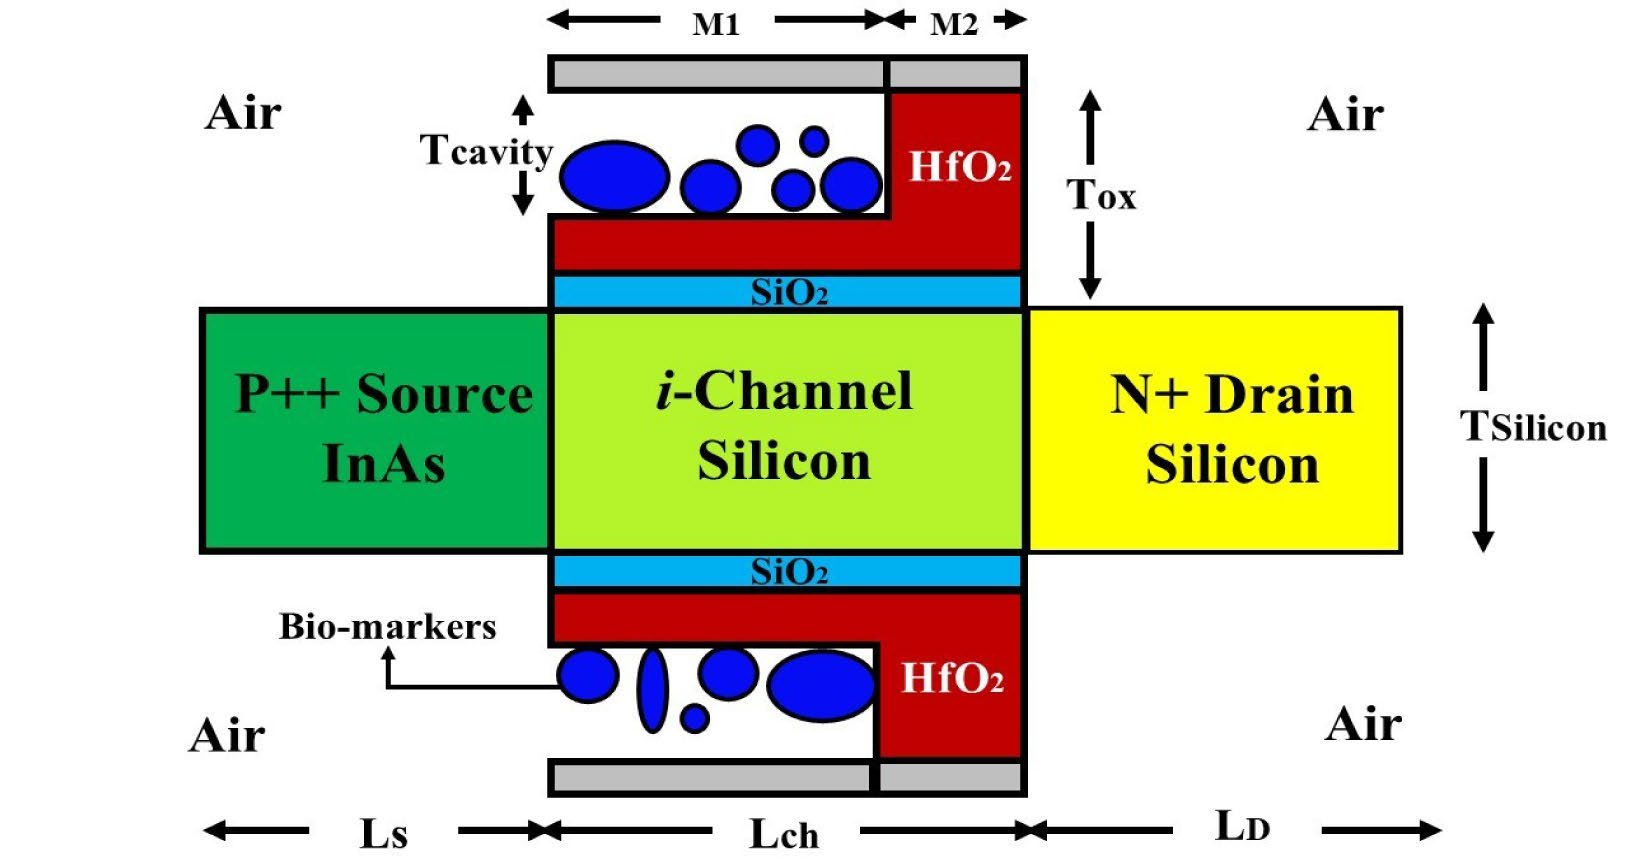
\includegraphics[width=0.85\columnwidth]{assets/images/faculty_psa_device.jpg}
    \captionof{figure}{Cross-section of the heterostructure oxide-engineered double-gate TFET biosensor.}
\end{minipage}
  \end{center}
\vspace{-0.35em}

  \subsection*{\centering\uppercase{Device and Simulation Model}}
  The structure is analysed with SILVACO ATLAS TCAD. Non-local BTBT, concentration- and field-dependent mobility, Fermi--Dirac statistics, Shockley--Read--Hall recombination, bandgap narrowing, trap-assisted tunnelling, and drift--diffusion transport are included. The transient Heiman model represents trap capture and emission during forward and reverse gate sweeps [1, 5].

  \noindent
  Calibration is performed against reported experimental characteristics of lateral p-type InAs--Si TFETs. Agreement is obtained using an interface-trap density of the order of $10^{12}\,\mathrm{cm}^{-2}$ at the Si--SiO$_2$ interface and a channel mobility near $590\,\mathrm{cm^2/(V\,s)}$. This calibration improves physical credibility, although it is not equivalent to fabricating and measuring the complete biosensor.

  \subsection*{\centering\uppercase{Fabrication Feasibility}}
  The proposed flow is informed by experimental lateral InAs--Si TFET integration using selective epitaxy and oxide templates [6]. A practical sequence would form the InAs source, silicon channel and drain, deposit the SiO$_2$/HfO$_2$ dielectric stack, define the dual-metal gate, etch the sensing cavities, and add a surface coating and linker chemistry for selective binding. Cavity etching and interface quality remain important fabrication risks because damage or roughness can increase the very traps examined in this work.
\end{multicols}

\begin{table}[tb]
\centering
\caption{Principal model dimensions and operating conditions.}
\small
  \setlength{\tabcolsep}{6pt}
  \renewcommand{\arraystretch}{1.3}
  \begin{tabular}{@{}>{\bfseries\RaggedRight\arraybackslash}p{0.28\textwidth}
                      >{\Centering\arraybackslash}p{0.20\textwidth}
                      >{\RaggedRight\arraybackslash}p{0.44\textwidth}@{}}
    \toprule
    \textbf{Parameter} & \textbf{Value} & \textbf{Purpose} \\
    \midrule
    Silicon body thickness & $10\,\mathrm{nm}$ & Nanoscale channel with double-gate control \\
    Oxide / cavity thickness & $11/8\,\mathrm{nm}$ & Gate stack and dielectric-modulation region \\
    Channel length & $40\,\mathrm{nm}$ & $30\,\mathrm{nm}$ M1 plus $10\,\mathrm{nm}$ M2 gate regions \\
    Source / drain doping & $10^{19}/5\times10^{18}\,\mathrm{cm}^{-3}$ & Degenerate p-type source and n-type drain \\
    Gate work functions & $3.8$ and $4.7\,\mathrm{eV}$ & Dual-material electrostatic engineering \\
    Gate / drain bias & $0$--$1.5\,\mathrm{V}$ / $1\,\mathrm{V}$ & Transfer sweep and readout condition \\
    Modelled interface traps & Up to $5\times10^{12}\,\mathrm{cm}^{-2}$ & Transient reliability and hysteresis analysis \\
    \bottomrule
  \end{tabular}
\end{table}
\vspace{-0.18em}

\begin{multicols}{2}
  \subsection*{\centering\uppercase{Fresh-Sensor Response}}
  Table~1 lists principal model dimensions and operating conditions.
  The electrostatic simulations show that increasing the cavity dielectric constant strengthens the electric field at the source--channel junction. For diseased-cell conditions, the tunnelling distance falls by roughly $70\%$ relative to the reference case, increasing BTBT rate and saturation drain current. The simulated switching ratio improves by several orders of magnitude, while the subthreshold slope becomes steeper for larger $\kappa$ values [1].

  \subsubsection*{Sensitivity Metrics}
  Drain-current sensitivity is defined relative to the air-filled cavity:
  \[
    S_{I_{\mathrm{ON}}}=\tfrac{I_{\mathrm{ON}}(\text{cell})}{I_{\mathrm{ON}}(\text{air})}.
  \]
  Subthreshold-slope sensitivity is
  \[
    S_{SS}=\tfrac{|SS(\text{cell})-SS(\text{air})|}{SS(\text{air})}.
  \]
  In the neutral-cell model, peak $S_{I_{\mathrm{ON}}}$ reaches approximately $1.11\times10^9$ for T47D at $V_G\approx1.05\,\mathrm{V}$. At a fixed $V_G=1.5\,\mathrm{V}$, T47D produces $S_{I_{\mathrm{ON}}}\approx7.77\times10^8$, while MCF-10A produces approximately $3.42\times10^5$. These large simulated differences motivate the use of drain current as a sensing signal.

  \noindent\begin{minipage}{\columnwidth}
  \subsubsection*{Effect of Fixed Cell Charge}
  Positive fixed charge near the cavity promotes inversion and shifts the transfer curve toward lower gate voltage; negative charge promotes accumulation and shifts it toward higher voltage. Fixed charge can therefore move the threshold and change sensitivity. The simulations distinguish this static shift from hysteresis: a fixed charge does not automatically create different forward and reverse curves.
  \end{minipage}

  \subsection*{\centering\uppercase{Trap-Induced Hysteresis}}
  Interface defects can capture electrons during an upward gate sweep and release them on a different timescale during the downward sweep. The resulting transfer curves no longer coincide.   Hysteresis width is measured at a chosen current criterion as
  \[
    HW=|V_{\mathrm{th,for}}-V_{\mathrm{th,rev}}|.
  \]
  A simplified dependence is
  \[
    HW\approx\tfrac{q f_t N_{it}}{C_{\mathrm{net}}},
  \]
  where $q$ is electronic charge, $f_t$ is trap occupancy, $N_{it}$ is interface-trap density, and $C_{\mathrm{net}}$ is the effective series capacitance.

  \begin{center}
\vspace{-0.5em}
\begin{minipage}{0.98\columnwidth}
\centering
    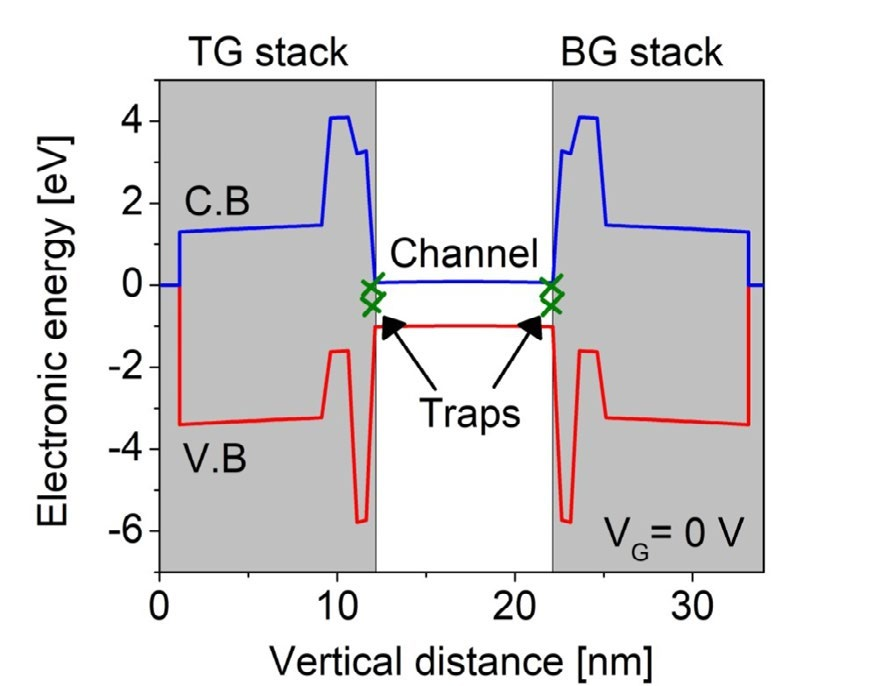
\includegraphics[width=0.82\columnwidth]{assets/images/faculty_psa_hysteresis.jpg}
    \captionof{figure}{Forward and reverse transfer curves defining hysteresis width for the T47D condition.}
\end{minipage}
  \end{center}
\vspace{-0.35em}

  \subsection*{\centering\uppercase{Sweep-Rate Dependence}}
  Sweep rate determines how long traps have to exchange charge with the channel. The study models a triangular gate waveform between $0$ and $1.5\,\mathrm{V}$. For T47D, hysteresis is approximately $10.2\,\mathrm{mV}$ at $1\,\mathrm{V/s}$, $16.3\,\mathrm{mV}$ at $0.1\,\mathrm{V/s}$, and $32.8\,\mathrm{mV}$ at $0.01\,\mathrm{V/s}$. A slow sweep allows more traps to capture and retain charge, increasing the difference between forward and reverse thresholds.

  \begin{center}
\vspace{-0.5em}
\begin{minipage}{0.98\columnwidth}
\centering
    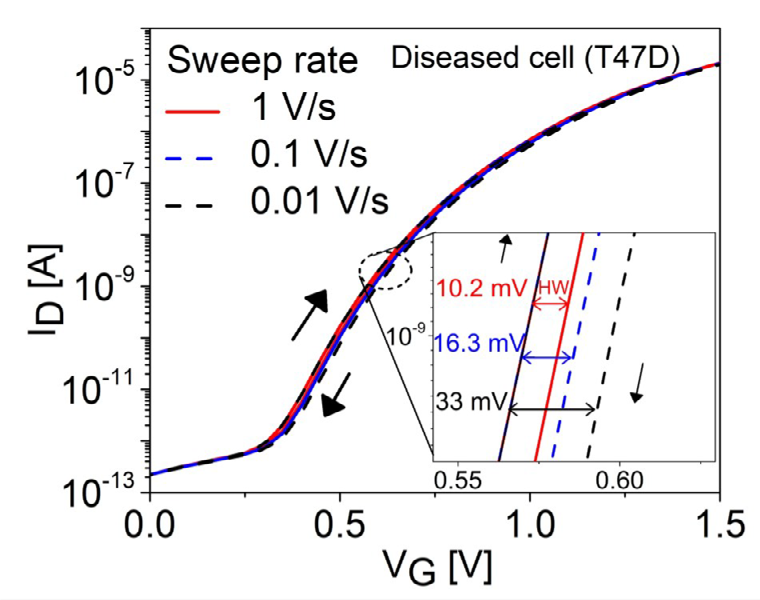
\includegraphics[width=0.84\columnwidth]{assets/images/faculty_psa_sweep_rate.png}
    \captionof{figure}{Simulated hysteresis increases as the gate sweep becomes slower.}
\end{minipage}
  \end{center}
\vspace{-0.35em}

  \subsection*{\centering\uppercase{Temperature and Trap Location}}
  At a fixed slow sweep rate, predicted hysteresis for the T47D condition rises from $32.8\,\mathrm{mV}$ at $300\,\mathrm{K}$ to $35.1\,\mathrm{mV}$ at $350\,\mathrm{K}$ and $40.2\,\mathrm{mV}$ at $400\,\mathrm{K}$. Higher temperature alters capture and emission times and increases thermal carrier velocity.

  \noindent
  Trap location also matters. The model compares defects at the crystalline InAs--Si heterojunction with those at the amorphous/crystalline Si--SiO$_2$ boundary. Across the investigated sweep rates, Si--SiO$_2$ traps produce larger hysteresis because their time-constant distribution interacts more strongly with the applied sweep. Reliability improvement therefore requires careful oxide growth, interface passivation, and low-damage cavity processing.

  \subsection*{\centering\uppercase{Damaged-Sensor Sensitivity}}
  Traps introduce recombination paths, reduce available channel carriers, and degrade on-current. The resulting drain-current sensitivity is lower than that of the fresh device for every modelled cell line. The study defines
  \[
    \text{Inaccuracy}=\left|
    \tfrac{S_{I_{\mathrm{ON}}}^{\mathrm{damaged}}-
    S_{I_{\mathrm{ON}}}^{\mathrm{fresh}}}
    {S_{I_{\mathrm{ON}}}^{\mathrm{fresh}}}
    \right|\times100\%.
  \]
  The predicted inaccuracy is about $97\%$ for MCF-10A, around $60\%$ for several intermediate diseased-cell conditions, and roughly $50\%$ for T47D. A sensor may therefore retain a seemingly large signal for a strongly coupled target while becoming unreliable near the healthy/disease decision boundary.

  \begin{center}
\vspace{-0.5em}
\begin{minipage}{0.98\columnwidth}
\centering
    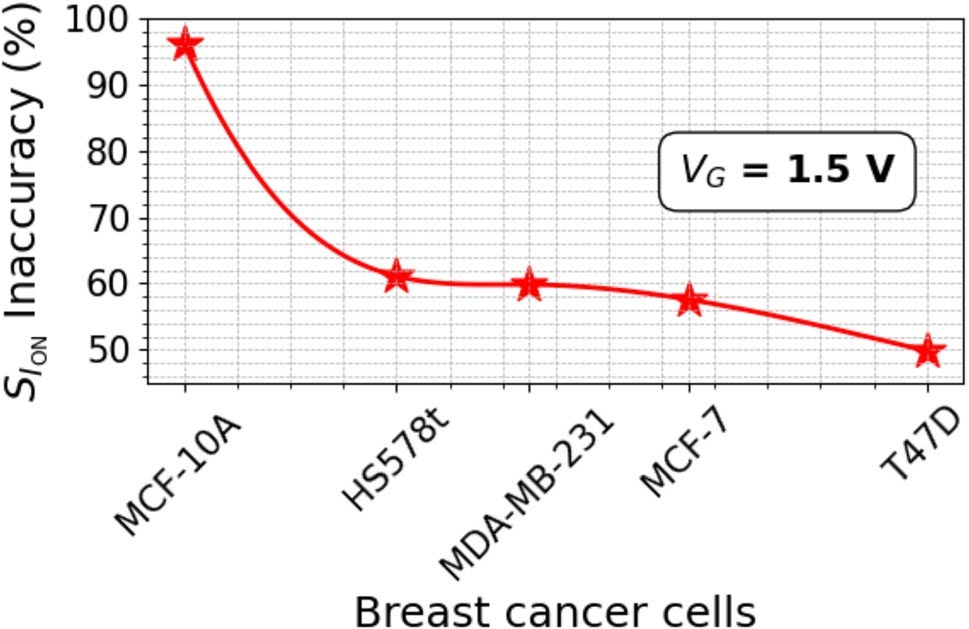
\includegraphics[width=0.85\columnwidth]{assets/images/faculty_psa_inaccuracy.jpg}
    \captionof{figure}{Sensitivity inaccuracy caused by trap degradation for the modelled cell conditions.}
\end{minipage}
  \end{center}
\end{multicols}

\begin{table}[t]
\centering
\caption{Key reliability results from the calibrated simulation study.}
\small
  \setlength{\tabcolsep}{6pt}
  \renewcommand{\arraystretch}{1.35}
  \begin{tabular}{@{}>{\bfseries\RaggedRight\arraybackslash}p{0.24\textwidth}
                      >{\Centering\arraybackslash}p{0.23\textwidth}
                      >{\RaggedRight\arraybackslash}p{0.45\textwidth}@{}}
    \toprule
    \textbf{Comparison} & \textbf{Predicted Result} & \textbf{Interpretation} \\
    \midrule
    T47D sweep rate: $1\rightarrow0.01\,\mathrm{V/s}$ & $HW:10.2\rightarrow32.8\,\mathrm{mV}$ & Slow measurement exposes more trap capture and delayed emission \\
    T47D temperature: $300\rightarrow400\,\mathrm{K}$ & $HW:32.8\rightarrow40.2\,\mathrm{mV}$ & Thermal activation increases trap participation \\
    Fixed positive cell charge, no switching traps & $HW\approx0$ & Static charge shifts threshold but does not create sweep-dependent hysteresis \\
    Si--SiO$_2$ versus InAs--Si traps & Larger $HW$ at Si--SiO$_2$ & Oxide-interface time constants dominate the simulated degradation \\
    MCF-10A fresh versus damaged sensitivity & Approximately $97\%$ inaccuracy & Reliability loss can hide or distort the healthy reference condition \\
    T47D fresh versus damaged sensitivity & $7.77\times10^8\rightarrow3.9\times10^8$ & Strong response remains, but absolute sensitivity is substantially reduced \\
    \bottomrule
  \end{tabular}
\end{table}
\vspace{-0.18em}

\begin{multicols}{2}
  \subsection*{\centering\uppercase{Sensitivity Versus Selectivity}}
  Table~2 summarizes key reliability results from the calibrated simulation study.
  Selectivity measures discrimination between the T47D target and other cell conditions. The damaged device can show a larger relative contrast for some comparisons even while its absolute current and sensitivity fall. This is not an improvement in overall sensing quality. A weak signal may appear relatively distinct yet remain difficult to measure accurately in the presence of noise, drift, device variability, and biological interference.

  \noindent
  Reliable benchmarking should therefore report the raw transfer curves, signal magnitude, sensitivity, selectivity, hysteresis, repeatability, noise, and calibration drift. Evaluating only one normalised metric can conceal device degradation.

  \subsection*{\centering\uppercase{Clinical and Experimental Limitations}}
  The reported results are calibrated TCAD predictions, not measurements from a fabricated H-OE-DG-TFET biosensor. No liquid-phase breast-cell assay is included. The assumed dielectric constants represent literature values and may vary with frequency, temperature, cell state, measurement method, surface coverage, and biological environment.

  \noindent
  A practical electrolyte creates an electric double layer and introduces biolayer capacitance, mobile ions, Debye screening, reference-electrode conditions, fluidic transport, non-specific adsorption, and surface-chemistry variability. These effects modify the effective capacitance and surface-potential coupling. Experimental work must also demonstrate selectivity through appropriate receptors and controls; dielectric contrast alone does not identify a cancer cell uniquely.

  \subsection*{\centering\uppercase{Design Guidance}}
  The study suggests several priorities for future devices:
  \begin{itemize}\justifying
    \item minimise Si--SiO$_2$ defect density through interface passivation and controlled processing;
    \item report gate sweep rate, direction, current criterion, temperature, and bias history with every hysteresis result;
    \item calibrate fresh and aged devices rather than assuming sensitivity remains constant;
    \item include liquid-gate electrostatics, receptor layers, ionic screening, and realistic biological noise;
    \item evaluate device-to-device variability and repeated measurement cycles;
    \item confirm the predicted response through fabrication and blinded biological testing.
  \end{itemize}

  \subsection*{\centering\uppercase{Conclusion}}
  The oxide-engineered InAs--Si double-gate TFET offers a promising simulated platform for dielectric-modulated breast-cancer sensing. Larger dielectric constants strengthen electrostatic coupling, shorten the tunnelling path, and increase drain-current sensitivity. The same device, however, is vulnerable to transient charge trapping at semiconductor interfaces.

  \noindent
  Trap-induced hysteresis depends strongly on measurement time and temperature, with the Si--SiO$_2$ interface producing the greatest degradation in the model. Sensitivity loss can be severe even when selectivity appears acceptable. The central lesson is that a biosensor cannot be judged by peak sensitivity alone: stability, hysteresis, inaccuracy, fabrication quality, measurement protocol, and experimental validation must be designed together.

  \subsection*{\centering\uppercase{References}}
  {\small
  \begin{justify}
    \begin{enumerate}[label={\relax[\arabic*]},leftmargin=*,labelsep=0.5em,itemsep=0.20em,parsep=0pt]
      \item R. Ghosh and P. Saha, “Modeling trap dynamics in oxide-engineered heterostructure TFETs for breast cancer detection,” \textit{Scientific Reports}, vol. 16, art. 3970, 2026.
      \item H. Im et al., “A dielectric-modulated field-effect transistor for biosensing,” \textit{Nature Nanotechnology}, vol. 2, no. 7, pp. 430--434, 2007.
      \item S. Shreya et al., “Core-shell junctionless nanotube tunnel field effect transistor: Design and sensitivity analysis for biosensing application,” \textit{IEEE Sensors Journal}, vol. 20, no. 2, pp. 672--679, 2020.
      \item M. Hussein et al., “Breast cancer cells exhibit specific dielectric signatures in vitro,” \textit{Scientific Reports}, vol. 9, art. 4681, 2019.
      \item F. Heiman and G. Warfield, “The effects of oxide traps on the MOS capacitance,” \textit{IEEE Transactions on Electron Devices}, vol. 12, no. 4, pp. 167--178, 1965.
      \item K. E. Moselund et al., “Lateral InAs/Si P-type tunnel FETs integrated on Si---Part 1: Experimental devices,” \textit{IEEE Transactions on Electron Devices}, vol. 63, no. 11, pp. 4233--4239, 2016.
      \item S. Sant et al., “Lateral InAs/Si P-type tunnel FETs integrated on Si---Part 2: Simulation study of the impact of interface traps,” \textit{IEEE Transactions on Electron Devices}, vol. 63, no. 11, pp. 4240--4247, 2016.
      \item R. Ghosh et al., “Theoretical insights into the impact of border and interface traps on hysteresis in monolayer MoS$_2$ FETs,” \textit{Microelectronic Engineering}, vol. 299, art. 112333, 2025.
      \item Silvaco, \textit{ATLAS User's Manual}, Santa Clara, CA, USA.
    \end{enumerate}
    \end{justify}}
\end{multicols}

\begin{center}
\begin{tcolorbox}[colback=SoftBlue, colframe=IEEEblue!70!black, boxrule=0.5pt, arc=0mm, left=3mm, right=3mm, top=2mm, bottom=2mm, width=0.92\textwidth]
\small\RaggedRight \textbf{\color{IEEEblue!75!black}Did you know?} — The human brain runs on roughly 20\,W while a state-of-the-art GPU can draw up to 700\,W, which is why neuromorphic chips compute with sparse spikes instead of dense clock-driven arithmetic.
\end{tcolorbox}
\end{center}

\begin{center}
  \section{\capitalisewords{Neuromorphic Computing Chips Inspired by the Human Brain}}
  Soumyadeep Sengupta, 1$^{st}$ Year, ECE
\end{center}
\vspace{-0.18em}

\setcounter{figure}{0}
\setcounter{table}{0}

\begin{multicols}{2}
  \begin{abstract}
    \bfseries
    Artificial Intelligence revolution is built on an unstated inefficiency, while the human brain performs complex discernment on approximately 20 watts, a state-of-the-art GPU draws up to 700 watts for similar workloads. Neuromorphic computing addresses this basic inconsistency by replicating the framework of biological neural networks directly in hardware by integrating memory and computation. Running only on incoming spike events, and learning through local synaptic rules rather than global backward propagation of errors. This report goes over the entire neuromorphic pipeline, from the biological neuron's threshold-firing mechanism to Spiking Neural Networks (SNNs) trained using surrogate gradient methods and Model Fusion Technology (MFT), continuing into silicon implementation on Intel's Loihi 2 and the billion-neuron Hala Point
    system. We go over the 2024--2025 state-of-the-art benchmarks, including SpikeYOLO achieving 66.2\%
    mAP@50 on COCO with \(5.7\times\) energy efficiency over equivalent ANNs, and Advanced SpikingYOLOX
    leveraging 2D-Spiking Transformers for object detection at ACM MM 2025 that confirm SNNs have crossed
    from research interests to competitive engineering. The 2026 University of Cambridge hafnium oxide
    memristive synapse breakthrough, providing a 70\% energy reduction using standard CMOS-compatible
    materials, is analysed alongside the critical integration challenge of linking spike-domain hardware with real-
    valued deep learning pipelines. With the neuromorphic market projected to reach \$61.48 billion by 2035 at a
    33.32\% CAGR, and neuromorphic chip patents rising 401\% in 2025 alone, this report demonstrates that computing modelled by the human brain is not a future possibility, it is an engineering reality.

    \vspace{1em}
    {\justifying\noindent\textbf{Keywords:} Neuromorphic Computing, Spiking Neural Networks, Surrogate Gradient, MFT Training, SpikeYOLO, SpikingYOLOX, Memristor, ANN-to-SNN Conversion, Loihi 2, Hala Point, Event-Driven AI.\par}
  \end{abstract}

  \subsection*{\centering\uppercase{INTRODUCTION}}
  There is a strange contradiction at the base of modern AI. The field's greatest ambition to replicate human intelligence is pursued using hardware fundamentally opposite to the organ it seeks to replicate. The human brain processes information across 86 billion neurons connected by 100 trillion synapses, running on roughly 20 watts of cellular power. The NVIDIA H100 GPU, today's AI workhorse, draws up to 700 watts under full load. At data-centre scale, this gap becomes critical. Global AI infrastructure is projected to consume 1,000 TWh of electricity yearly by 2026 comparable to Japan's total national energy consumption.

  \noindent
  This is not merely an environmental concern, it is an engineering ceiling. As AI models scale toward hundreds of trillions of new limits, power consumption threatens to become the front running issue on further capability growth. The solution, many researchers argue, has been operating inside human skulls for millions of years.

  \noindent
  Neuromorphic computing, first theorized by Carver Mead at Caltech in the 1980s proposes the idea of building chips that mirror biological neural networks structurally and programmatically. Unlike conventional von Neumann architectures, which continuously shift data between separate memory and processing units, neuromorphic systems co-locate computation and storage. These activate only on spike events, and learn
  through local synaptic adaptation. Between 2024 and 2026, the initial model crossed a decisive onset from laboratory demonstration to competitive benchmarks, from exotic materials to CMOS-compatible fabrication, and from academic precursor to the world's largest deployed AI system by neuron count.

  \subsection*{\centering\uppercase{Biological Foundations: From Neuron to Circuit}}
  \subsubsection*{Threshold-Fired Spike Coding}
  A biological neuron brings together electrochemical inputs across its dendritic membrane. Only when
  accumulated charge crosses a critical upper limit, does it emit a different action potential. It sends a
  spike down its axon to connected neurons. This \textbf{all-or-nothing}, action-driven mechanism encrypts
  information in spike timing and rate, not continuous amplitude. The result stands out as zero
  computation during silence, and information processing only when something in the environment
  actually changes.

  \noindent
  Neuromorphic chips replicate this using \textbf{Leaky Integrate-and-Fire (LIF)} neurons. The most widely
  implemented spiking neuron model. Each LIF unit accumulates input charge as membrane
  potential \(V_m\), decays it with a leak term \(\tau\), and emits a spike when \(V_m\) exceeds threshold \(V_{\mathrm{th}}\). It
  immediately resets afterwards.

  \noindent
  The \textbf{Dynamic Threshold LIF (DT-LIF)} variant, suggested in 2025, dynamically adjusts \(V_{\mathrm{th}}\) based on
  incremental membrane potential, improving inference speed and increasing object detection accuracy
  on the \textbf{Prophesee Gen1} dataset by \textbf{25.2\%} over standard LIF implementations.

  \subsubsection*{Synaptic Plasticity: The Learning Synapse}
  Biological synapses strengthen or weaken through \textbf{Spike-Timing-Dependent Plasticity (STDP)}: if a
  presynaptic neuron fires just before a postsynaptic one, the synapse strengthens after, it weakens. This
  local, unsupervised rule requires no global loss function and no backpropagation signal. Hence, the
  synapse is the learning unit. Memristive (devices or materials that exhibit ``memristance'') device are
  two-terminal elements whose resistance history mirrors synaptic weight history are the hardware
  implementation of this principle.

  \subsection*{\uppercase{Training SNNs: The Surrogate Gradient Revolution}}
  \subsubsection*{The Non-Differentiability Problem}
  For a long period of time, SNNs could not be trained with standard backpropagation. This issue occurred
  because the spike function, a binary step has zero gradient almost everywhere. Hence, making gradient-based
  weight updates that were mathematically undefined. This "dead gradient" problem restricted SNNs to basic
  architectures trained by biologically-motivated but limited local rules like STDP.

  \noindent
  The field's breakthrough came through \textbf{surrogate gradient methods}, replacing the non-differentiable spike
  function with a smooth, differentiable approximation during the backward pass only, while preserving true
  binary spikes during forward computation. This allows deep SNNs to be trained end-to-end with
  backpropagation-through-time (BPTT), unlocking architectures as deep as ResNet-34 on large-scale datasets.

  \subsubsection*{Model Fusion Technology (MFT): Best of Both Worlds}
  The 2024--2025 state-of-the-art training framework is \textbf{Model Fusion Technology (MFT)}, which hybridizes two previously competing approaches:
  \begin{itemize}
    \item \textbf{Direct Training (STBP):} Trains SNNs from scratch using surrogate gradients high accuracy but slow convergence and high time-step requirements.
    \item \textbf{ANN-to-SNN Conversion:} Pre-trains an ANN, then converts activations to spike rates fast but incurs large time-step overhead (100--1000+ steps) for accurate conversion.
  \end{itemize}
  MFT fuses both an ANN backbone is pre-trained conventionally, a \textbf{Batch-Matched Integrate-and-Fire (BM-
  IF) neuron} simplifies the conversion stage and reduces conversion error, and surrogate-gradient fine-tuning
  then refines the hybrid network. Results on this approach are striking:

  Table~1 compares MFT-based SNN and ANN-to-SNN conversion on key benchmarks.

\begin{center}
\vspace{-0.5em}
\begin{minipage}{0.98\columnwidth}
\centering
    \captionof{table}{MFT-based SNN vs. ANN-to-SNN conversion on key benchmarks}
    \scriptsize
    \setlength{\tabcolsep}{3pt}
    \renewcommand{\arraystretch}{1.25}
    \begin{tabular}{@{}>{\RaggedRight\arraybackslash}p{0.28\columnwidth}>{\RaggedRight\arraybackslash}p{0.31\columnwidth}>{\RaggedRight\arraybackslash}p{0.31\columnwidth}@{}}
      \toprule
      \textbf{Metric} & \textbf{ANN-to-SNN Conversion} & \textbf{MFT-based SNN} \\
      \midrule
      Inference time steps & \(512\text{--}1250\times\) baseline & \(1\times\) (\(512\text{--}1250\times\) reduction) \\
      ImageNet-1K Accuracy & \(\sim 65\%\) (SOTA) & 67.38\% (new SOTA) \\
      Remote sensing (UCM) & \(\sim 97\%\) & 99.62\% \\
      Remote sensing (AID) & \(\sim 96\%\) & 98.81\% \\
      Convergence speed & Slow (STBP) & Significantly faster \\
      \bottomrule
    \end{tabular}
\end{minipage}
  \end{center}

  Additionally, \textbf{Differential Coding} (ICML 2025) advances ANN-to-SNN conversion further by
  transmitting changes in spike rate information rather than absolute rates---reducing total spike count and
  energy while achieving state-of-the-art accuracy, including \textbf{75.12\% on ImageNet with only 4-time steps}.

  \subsection*{\uppercase{Object Detection: SNNs Enter the Real World}}
  \subsubsection*{SpikeYOLO (ECCV 2024)}
  SpikeYOLO, presented at ECCV 2024, demonstrated that naive conversion of YOLO-series architectures to
  spiking equivalents causes spike degradation---complex module designs suppress spike propagation through
  deep layers. SpikeYOLO resolved this by simplifying the backbone with meta SNN blocks optimized for sparse
  spike flow and designing a new neuron activating integer values during training while extending virtual
  timesteps during inference. On the COCO dataset, it achieved 66.2\% mAP@50, which is 15.0 percentage points above the prior SNN
  state of the art; on the Gen1 neuromorphic dataset, it achieved \(5.7\times\) greater energy efficiency than an equivalent ANN.

  \subsubsection*{Advanced SpikingYOLOX (ACM MM 2025)}
  Advanced SpikingYOLOX extended SNN-based detection further using two architectural innovations: Spike-based Partial Self-Attention (SPSA), which selectively applies attention to high-information spike channels
  reducing computational overhead, and a 2D-Spiking Transformer that processes spatial and temporal spike
  dimensions jointly. Together, these bring transformer-class feature extraction into the spike domain---
  delivering ANN-competitive accuracy while retaining neuromorphic energy efficiency. This paper effectively
  closes the argument: on event-driven, temporally rich data, SNNs no longer merely approximate ANNs---they
  surpass them.

  \subsection*{\centering\uppercase{Hardware: From Loihi 2 to the Hafnium Breakthrough}}
  \subsubsection*{Intel Loihi 2 and Hala Point}
  Intel's \textbf{Loihi 2}, fabricated on the Intel 4 process node, integrates 2.3 billion transistors in \(31\,\mathrm{mm}^2\) of silicon,
  simulating 1 million programmable neurons per chip with up to \(10\times\) faster learning than its predecessor.
  The \textbf{Hala Point} system at Sandia National Laboratories scales this to \textbf{1,152 Loihi 2 chips}, achieving 1.15
  billion simulated neurons, 20 Peta operations per second, inference \textbf{\(50\times\) faster} than GPU equivalents, and \textbf{\(100\times\) lower power} on optimization workloads.

  \begin{center}
\vspace{-0.5em}
\begin{minipage}{0.98\columnwidth}
\centering
    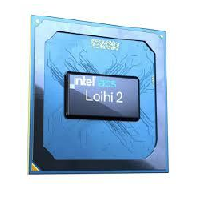
\includegraphics[width=0.65\columnwidth]{assets/images/Intel Lohi 2.png}
    \captionof{figure}{Intel Loihi 2}
\end{minipage}
  \end{center}
\vspace{-0.35em}

  \subsubsection*{The Cambridge Hafnium Oxide Memristor (2026)}
  The most commercially significant 2026 hardware development is the \textbf{University of Cambridge's hafnium
  oxide (\(\mathrm{HfO_2}\)) memristive synapse}. Unlike prior memristors relying on unstable conductive filament formation,
  this device exploits engineered \textbf{p-n heterointerfaces} between strontium-titanium-doped \(\mathrm{HfO_2}\) layers for
  deterministic, repeatable switching. Key measured properties:
  \begin{itemize}
    \item \textbf{70\% AI energy reduction} vs. conventional digital hardware.
    \item Switching currents \(\leq \mathbf{10^{-8}\,A}\)---one million times lower than standard oxide memristors.

    \item \textbf{Hundreds of stable conductance levels} for high-precision analogue in-memory computation

    \item Robust across \textbf{tens of thousands of switching cycles}.
  \end{itemize}
  The decisive commercial advantage: \(\mathrm{HfO_2}\) is already a standard gate dielectric in sub-10nm CMOS processes,
  meaning these synapses require \textbf{no new foundry infrastructure}---the single largest barrier to memristor
  commercialization, now eliminated.

  \begin{center}
\vspace{-0.5em}
\begin{minipage}{0.98\columnwidth}
\centering
    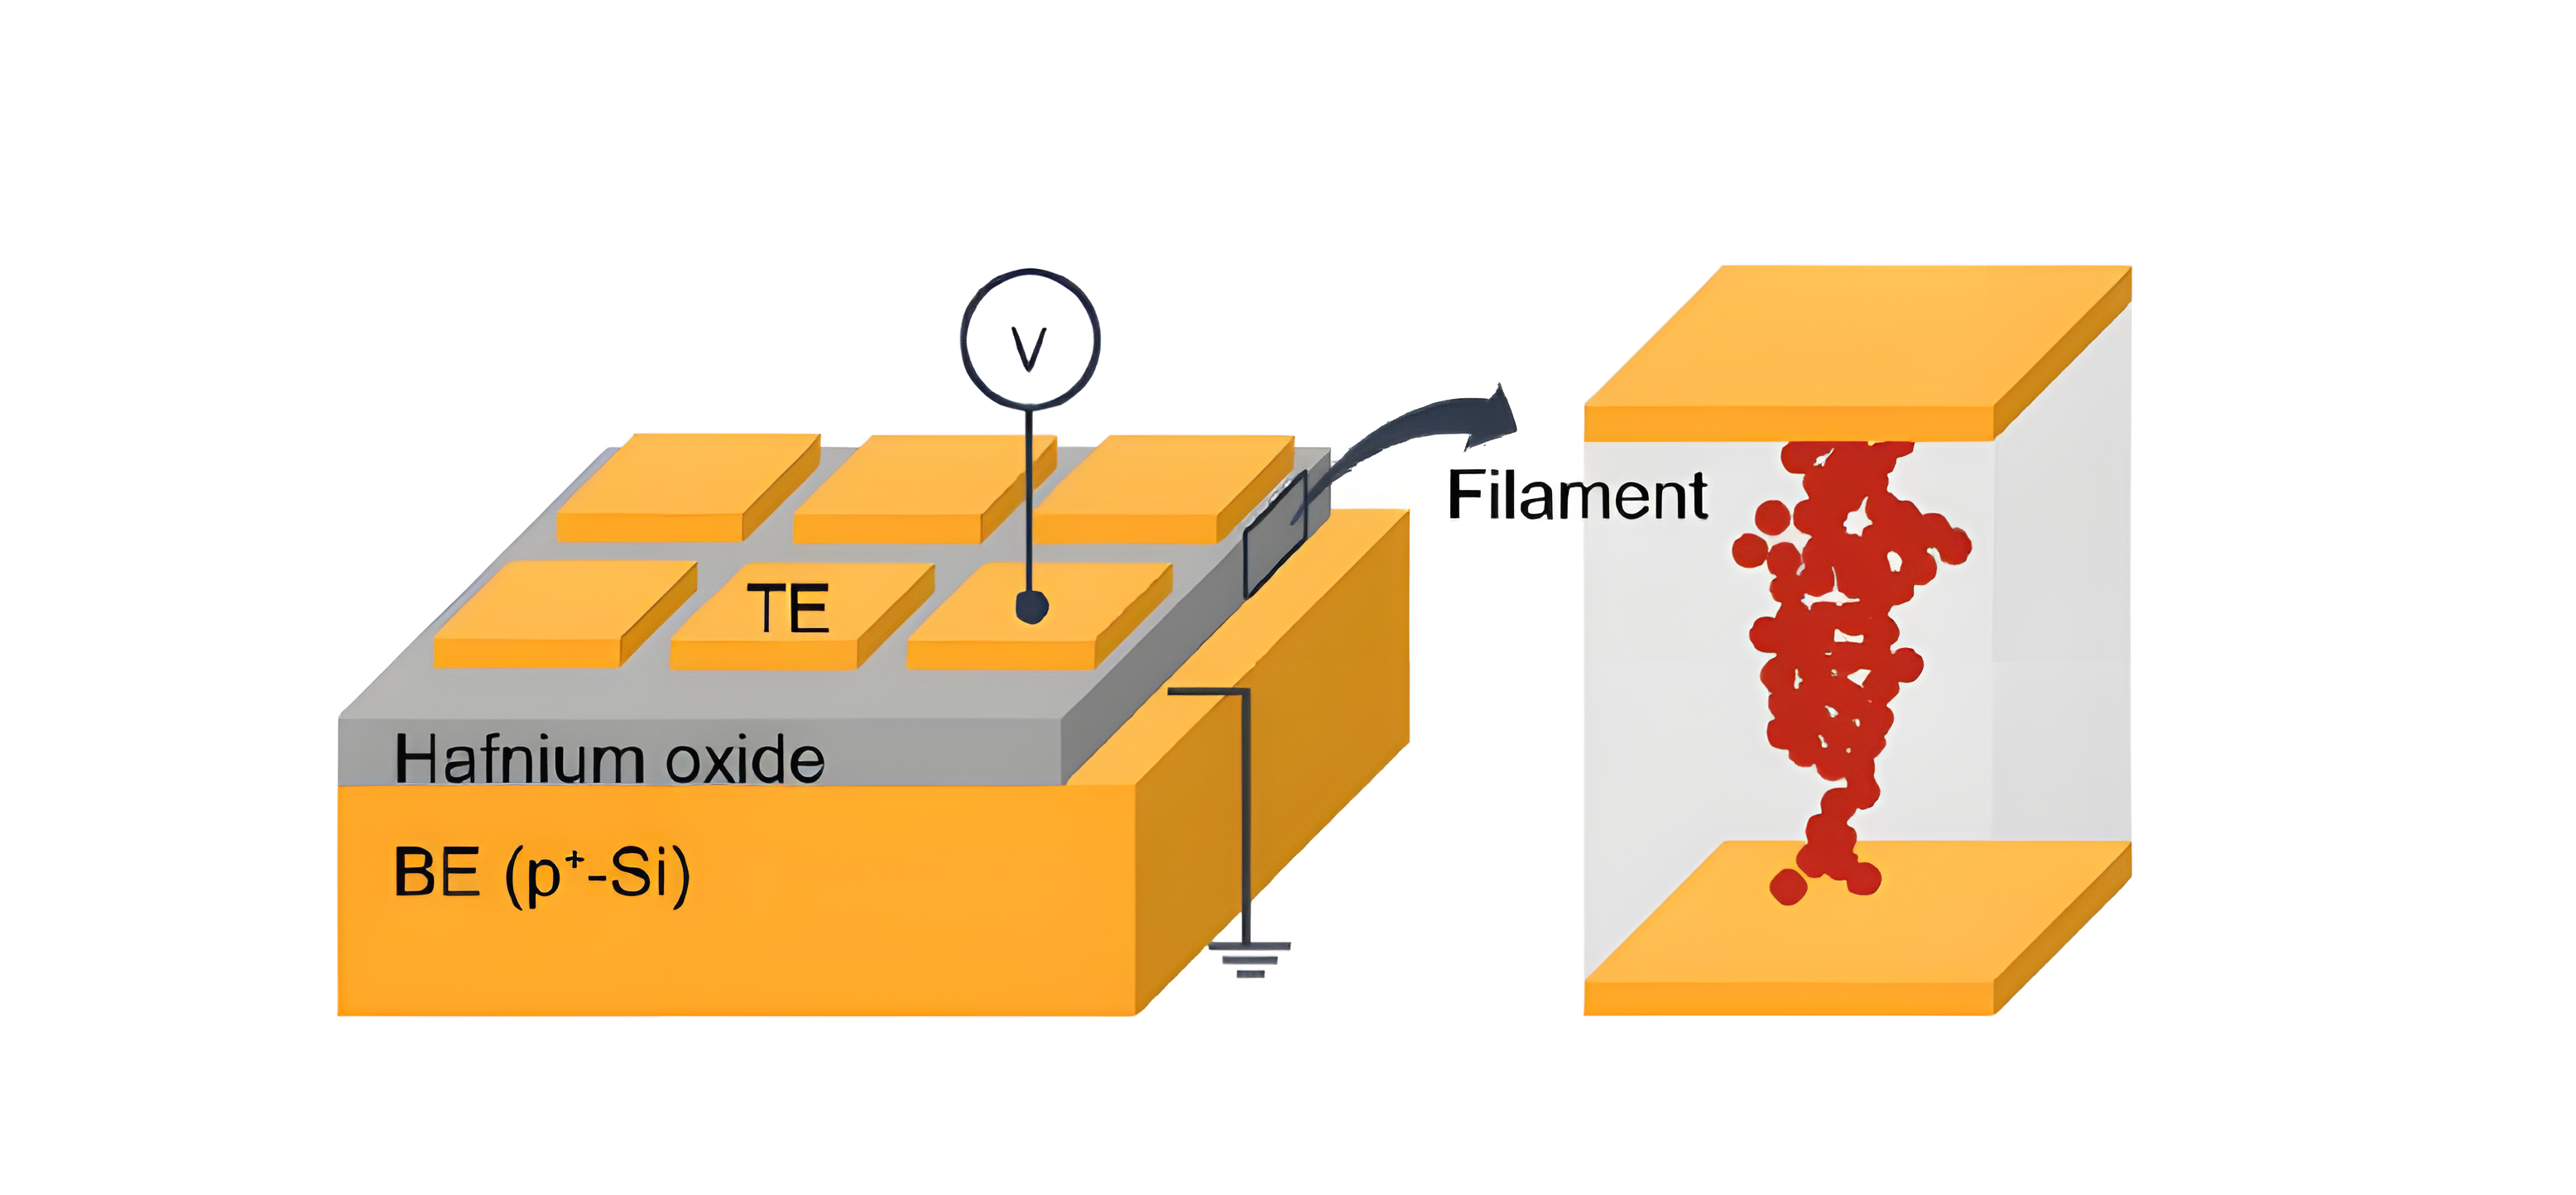
\includegraphics[width=0.85\columnwidth]{assets/images/Hafnium Oxide Memristor.png}
    \captionof{figure}{Hafnium Oxide Memristor}
\end{minipage}
  \end{center}
\vspace{-0.35em}

  \subsubsection*{The Integration Challenge: Bridging Spikes and Silicon Pipelines}
  Deploying neuromorphic accelerators within real engineering systems requires solving a fundamental interface
  problem: \textbf{neuromorphic hardware speaks in spikes; conventional software speaks in floating-point
  numbers}.

  \noindent
  The practical integration pipeline involves three stages:
  \begin{enumerate}
    \item \textbf{Encoding:} Real-valued sensor data (images, audio, signals) must be converted to spike trains---either
      via Poisson rate encoding, temporal coding, or, most efficiently, the differential coding scheme from
      ICML 2025
    \item \textbf{Processing:} The spiking accelerator (e.g., Loihi 2) processes the spike representation using on-chip
      LIF neurons and local learning rules
    \item \textbf{Decoding:} Output spike patterns must be decoded back to class labels, regression outputs, or control
      signals usable by downstream conventional systems
  \end{enumerate}

  \subsection*{\centering\uppercase{Market Trajectory and Commercialization Roadmap}}
  The commercial momentum behind neuromorphic computing is unambiguous and accelerating. The global
  market is projected to grow from \textbf{\$2.6 billion (2024) to \$61.48 billion by 2035} at a CAGR of \textbf{33.32\%}---
  among the fastest expansion trajectories in semiconductor history. Patent filings surged \textbf{401\% through early
  2026} with 596 filings recorded, driven by Intel, IBM, Samsung, and emerging neuromorphic startups.

  \noindent
  \begin{justify}
    The \textbf{2025 Neuromorphic Computing Roadmap} outlines three commercialization phases:
    \begin{itemize}
      \item \textbf{2025--2027:} Narrow-task edge deployment---always-on sensing, anomaly detection, IoT.
      \item \textbf{2027--2030:} Hybrid neuromorphic-GPU co-processors---SNN accelerators handling temporal data within conventional AI pipelines.
      \item \textbf{2030+:} Fully autonomous neuromorphic AI workloads with standardized programming models.
    \end{itemize}
  \end{justify}
  The roadmap explicitly identifies \textbf{benchmark standardization} as the field's highest-priority systemic challenge
  without MLPerf-equivalent metrics for SNNs, hardware vendors cannot make credible performance claims to
  enterprise buyers.
  \subsection*{\centering\uppercase{Conclusion}}
  Neuromorphic computing has crossed from architectural curiosity to measurable engineering reality. In 2024--2025,
  SNNs trained with surrogate gradients and MFT achieved ImageNet accuracies competitive with
  conventional deep learning. SpikeYOLO delivered object detection accuracy 15\% above prior SNN state-of-the-
  art with \(5.7\times\) energy savings. Advanced SpikingYOLOX brought transformer-class capability to spike-domain
  vision. On the hardware side, Hala Point's billion-neuron system operates at \(100\times\) lower power than GPU
  equivalents, while Cambridge's hafnium oxide memristors offer a 70\% energy cut using foundry-compatible
  materials.

  \noindent
  The remaining challenges memristor thermal stability, SNN algorithm scalability to transformer-scale models,
  and software toolchain fragmentation are real but tractable, with active research on each front in 2025 and 2026.
  For the electronics engineer of tomorrow, neuromorphic computing is no longer a specialization to consider. It is
  a foundation to master. The brain did not evolve over millions of years only to be ignored by its own imitations.

  \subsection*{\centering\uppercase{References}}
  \begin{justify}
  \Urlmuskip=0mu plus 1mu\relax
  \begin{enumerate}
    \item X. Luo et al., "Integer-Valued Training and Spike-Driven Inference Spiking Neural Network for High-
      Performance Object Detection," in Proc. ECCV, 2024. [Online]. Available:
      \url{https://eccv.ecva.net/virtual/2024/poster/150}

    \item ACM, "Advanced SpikingYOLOX: Extending Spiking Neural Network on Object Detection with
      Spike-based Partial Self-Attention and 2D-Spiking Transformer," in Proc. ACM MM, 2025. DOI:
      \url{10.1145/3746027.3754854}

    \item Y. Wang et al., "Deep Spiking Neural Networks Based on Model Fusion Technology," Engineering
      Applications of AI, Feb. 2025. DOI: \url{10.1016/j.engappai.2024.109873}

    \item ICML, "Differential Coding for Training-Free ANN-to-SNN Conversion," in Proc. ICML, 2025.
      [Online]. Available: \url{https://icml.cc/virtual/2025/poster/45408}

    \item OpenReview, "Error-Free ANN-to-SNN Conversion for Extreme Edge Efficiency," Jan. 2025.
      [Online]. Available: \url{https://openreview.net/forum?id=GTzP2GC7NR}

    \item Intel Corporation, "Intel Builds World's Largest Neuromorphic System---Hala Point," Intel
      Newsroom, Apr. 2024. [Online]. Available: \url{https://newsroom.intel.com}

    \item University of Cambridge, "\(\mathrm{HfO_2}\)-based Memristive Synapses via Asymmetric p-n
      Heterointerfaces," Science Advances, Mar. 2026.
  \end{enumerate}
  \end{justify}
\end{multicols}

\begin{center}
\begin{tcolorbox}[colback=SoftBlue, colframe=IEEEblue!70!black, boxrule=0.5pt, arc=0mm, left=3mm, right=3mm, top=2mm, bottom=2mm, width=0.92\textwidth]
\small\RaggedRight \textbf{\color{IEEEblue!75!black}Did you know?} — Shor's algorithm could break 2048-bit RSA in hours on a fault-tolerant quantum computer, but today's noisy qubits are far from that scale.
\end{tcolorbox}
\end{center}

\begin{center}
  \section{\capitalisewords{Beyond RSA/ECDSA: the future of post-quantum cryptography}}
  Sreejit Roy Chowdhury, 1$^{st}$ Year, ECE
\end{center}

\setcounter{figure}{0}

\begin{multicols}{2}
  \begin{abstract}
    \bfseries
    The rapid advancement of quantum computing poses a significant threat to classical cryptographic
    systems such as RSA and Elliptic Curve Digital Signature Algorithm (ECDSA), which form the foundation of
    modern digital security. Quantum algorithms, particularly Shor’s algorithm, have the potential to efficiently
    solve the mathematical problems underlying these cryptographic techniques, thereby compromising the
    confidentiality, integrity, and authenticity of digital communications. Post-Quantum Cryptography (PQC) has
    emerged as a promising solution to address these challenges by developing cryptographic algorithms that are
    resistant to attacks from both classical and quantum computers.

    \noindent
    This paper presents an overview of post-quantum cryptography, its importance in the era of quantum computing,
    and the major categories of quantum-resistant algorithms, including lattice-based, hash-based, code-based, and
    multivariate cryptographic systems. The study also highlights the standardization efforts led by the National
    Institute of Standards and Technology (NIST) and discusses widely recognized algorithms such as CRYSTALS-
    Kyber and CRYSTALS-Dilithium. Furthermore, the paper examines the practical challenges associated with the
    implementation and migration of PQC in real-world systems. The objective of this work is to provide a
    comprehensive understanding of the need for quantum-safe security mechanisms and the future direction of
    cryptographic research in the post-quantum era.

    \vspace{1em}
    {\justifying\noindent\textbf{Keywords:} Post-Quantum Cryptography, Quantum Computing, RSA, ECDSA, Shor’s Algorithm,
    Quantum-Resistant Security, Cryptography, NIST, CRYSTALS-Kyber, CRYSTALS-Dilithium.\par}
  \end{abstract}

  \subsection*{\centering\uppercase{INTRODUCTION}}
  In today’s digital world, cryptography plays a major role in protecting communication, online transactions,
  banking systems, passwords, and cryptocurrencies such as Bitcoin. Every time a user sends a message, logs into
  a website, or makes an online payment, cryptographic algorithms work in the background to keep the
  information safe from attackers.Modern internet security mainly depends on classical cryptographic systems
  such as RSA and Elliptic Curve Digital Signature Algorithm (ECDSA). RSA is a public-key cryptographic
  algorithm that secures communication using very large prime numbers, while ECDSA uses mathematical
  properties of elliptic curves to create secure digital signatures. These algorithms are currently trusted because
  classical computers require an extremely long time to solve the mathematical problems behind them.

  \noindent
  For example, Bitcoin uses ECDSA to protect wallet ownership and digital signatures. A Bitcoin wallet address
  is linked to a private key, and only the owner of that private key can authorize transactions. Bitcoin also uses the
  SHA-256 hashing algorithm to secure blocks and maintain the integrity of the blockchain. At present, breaking
  these systems using ordinary computers is practically impossible due to the astronomically large search space of
  \(2048^{12}\) combinations of seed phrases. However, the development of quantum computers has created new
  concerns in the field of cybersecurity. Unlike classical computers that process information using bits (0 or 1),
  quantum computers use qubits, which can exist in multiple states simultaneously. In the future, large-scale
  quantum computers with stable logical qubits may become powerful enough to solve certain mathematical
  problems much faster than classical computers. Thus, the need to bring Quantum-resistant security measures
  increases each passing day.

  \subsection*{\centering\uppercase{Public-Key Cryptography: RSA and ECDSA Foundations}}
  RSA and ECDSA are widely used public-key cryptographic systems that secure modern digital
  communication, online banking, secure web services, and cryptocurrencies such as Bitcoin. Their
  security is based on mathematical problems that are computationally difficult for classical computers.

  \noindent
  RSA is based on number theory and relies on the difficulty of factoring a large composite number into
  its prime factors. A public key is used for encryption, while a mathematically related private key is
  used for decryption. Although key generation is straightforward, breaking the system without the
  private key is infeasible because factoring large integers becomes extremely time-consuming as key
  sizes increase.

  \begin{center}
\vspace{-0.5em}
\begin{minipage}{0.98\columnwidth}
\centering
    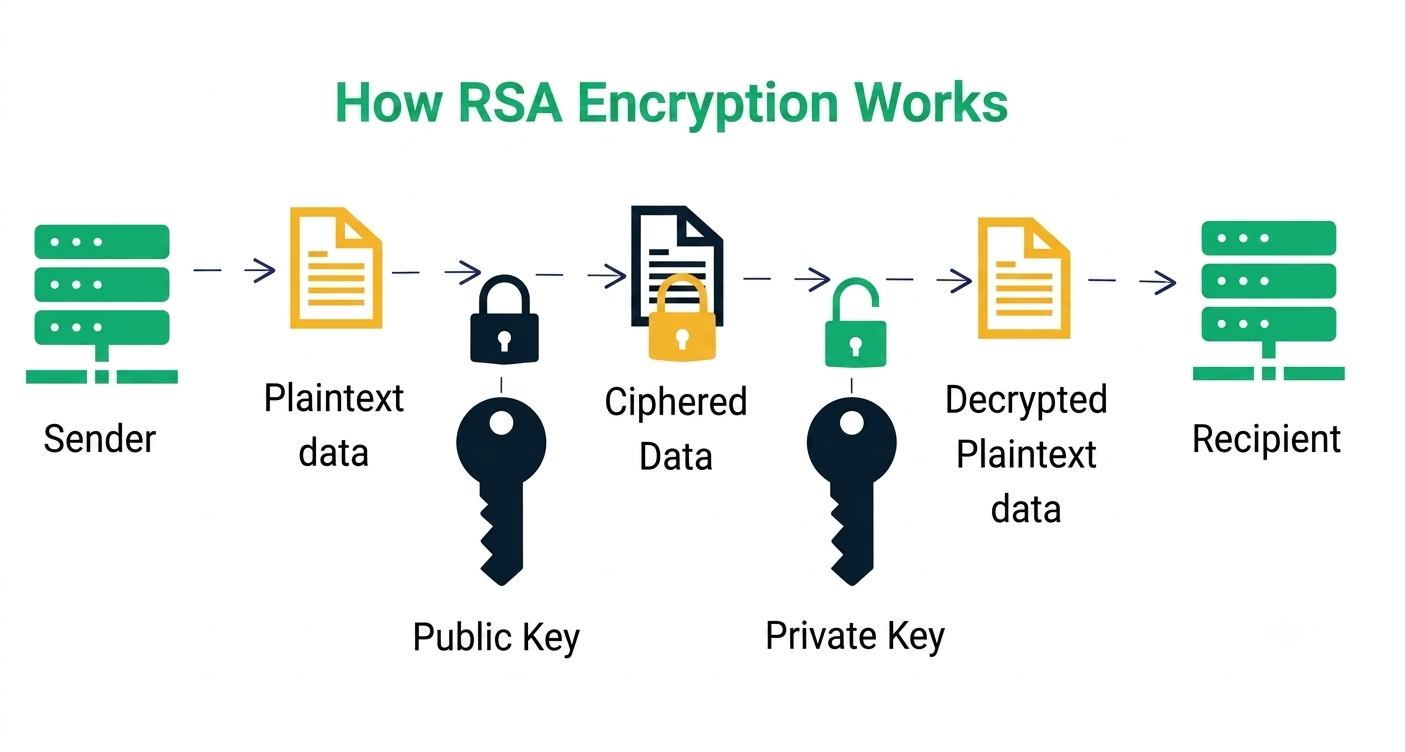
\includegraphics[width=0.9\columnwidth]{assets/images/RSA.png}
    \captionof{figure}{RSA}
\end{minipage}
  \end{center}

  ECDSA is based on elliptic curve cryptography over finite fields. A private key is a randomly selected
  number, and the corresponding public key is generated using elliptic curve point multiplication with a
  fixed generator point (G). Digital signatures are created using cryptographic hashing combined with
  elliptic curve operations, and verification is possible without revealing the private key. The security of
  ECDSA depends on the elliptic curve discrete logarithm problem, which makes it computationally
  infeasible to derive the private key from the public key using classical computing methods.

  \noindent
  Both RSA and ECDSA are widely deployed in real-world systems, including HTTPS/TLS protocols,
  secure messaging, and blockchain-based cryptocurrencies like Bitcoin.

  \noindent
  However, their security is based on mathematical hardness assumptions rather than absolute
  guarantees. This means that future advancements in quantum computing could potentially weaken
  these systems by solving their underlying mathematical problems more efficiently, motivating the
  development of post-quantum cryptography.

  \begin{center}
\vspace{-0.5em}
\begin{minipage}{0.98\columnwidth}
\centering
    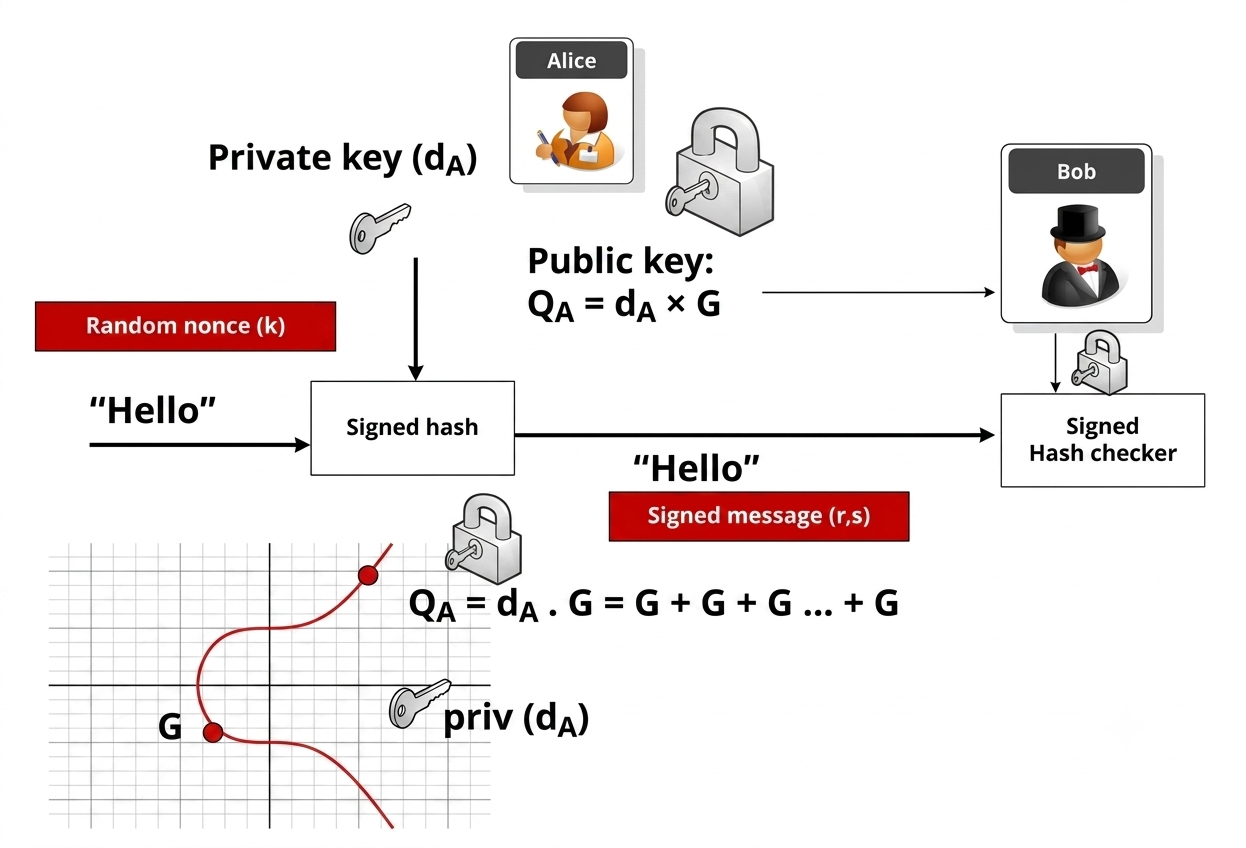
\includegraphics[width=0.9\columnwidth]{assets/images/ECDSA.png}
    \captionof{figure}{ECDSA}
\end{minipage}
  \end{center}

  With ECDSA, Alice will sign a message with her private key (d), and then Bob will use her public
  key to verify that she signed the message (and that the message has now changed):

  \noindent
  Alice signs the message with the following:
  \begin{enumerate}
    \item Create a hash of the message \(e=\operatorname{HASH}(m)\).
    \item Let \(h\) be the \(L_n\) be the leftmost bits of \(e\), \(L_n\) has a bit length of the group order \(N\).
    \item Create a random number \(k\) which is between \(1\) and \(N-1\).
    \item Calculate a point on the curve as \((x_1,y_1)=k\times G\).
    \item Calculate \(r=x_1\pmod N\). If \(r=0\), go back to Step 3.
    \item Calculate \(s=k^{-1}(h+r d_A)\pmod N\). If \(s=0\), go back to Step 3.
    \item The signature is the pair \((r,s)\).
  \end{enumerate}

  Bob will check with:
  \begin{enumerate}
    \item Create a hash of the message \(e=\operatorname{HASH}(m)\).
    \item Let \(h\) be the \(L_n\) leftmost bits of \(e\).
    \item Calculate \(c=s^{-1}\pmod N\).
    \item Calculate \(u_1=h\cdot c\pmod N\) and \(u_2=r\cdot c\pmod N\).
    \item Calculate the curve point \((x_1,y_1)=u_1\times G+u_2\times Q_A\). If \((x_1,y_1)=\mathcal{O}\), then the signature is
      invalid.
  \end{enumerate}

  \begin{center}
\vspace{-0.5em}
\begin{minipage}{0.98\columnwidth}
\centering
    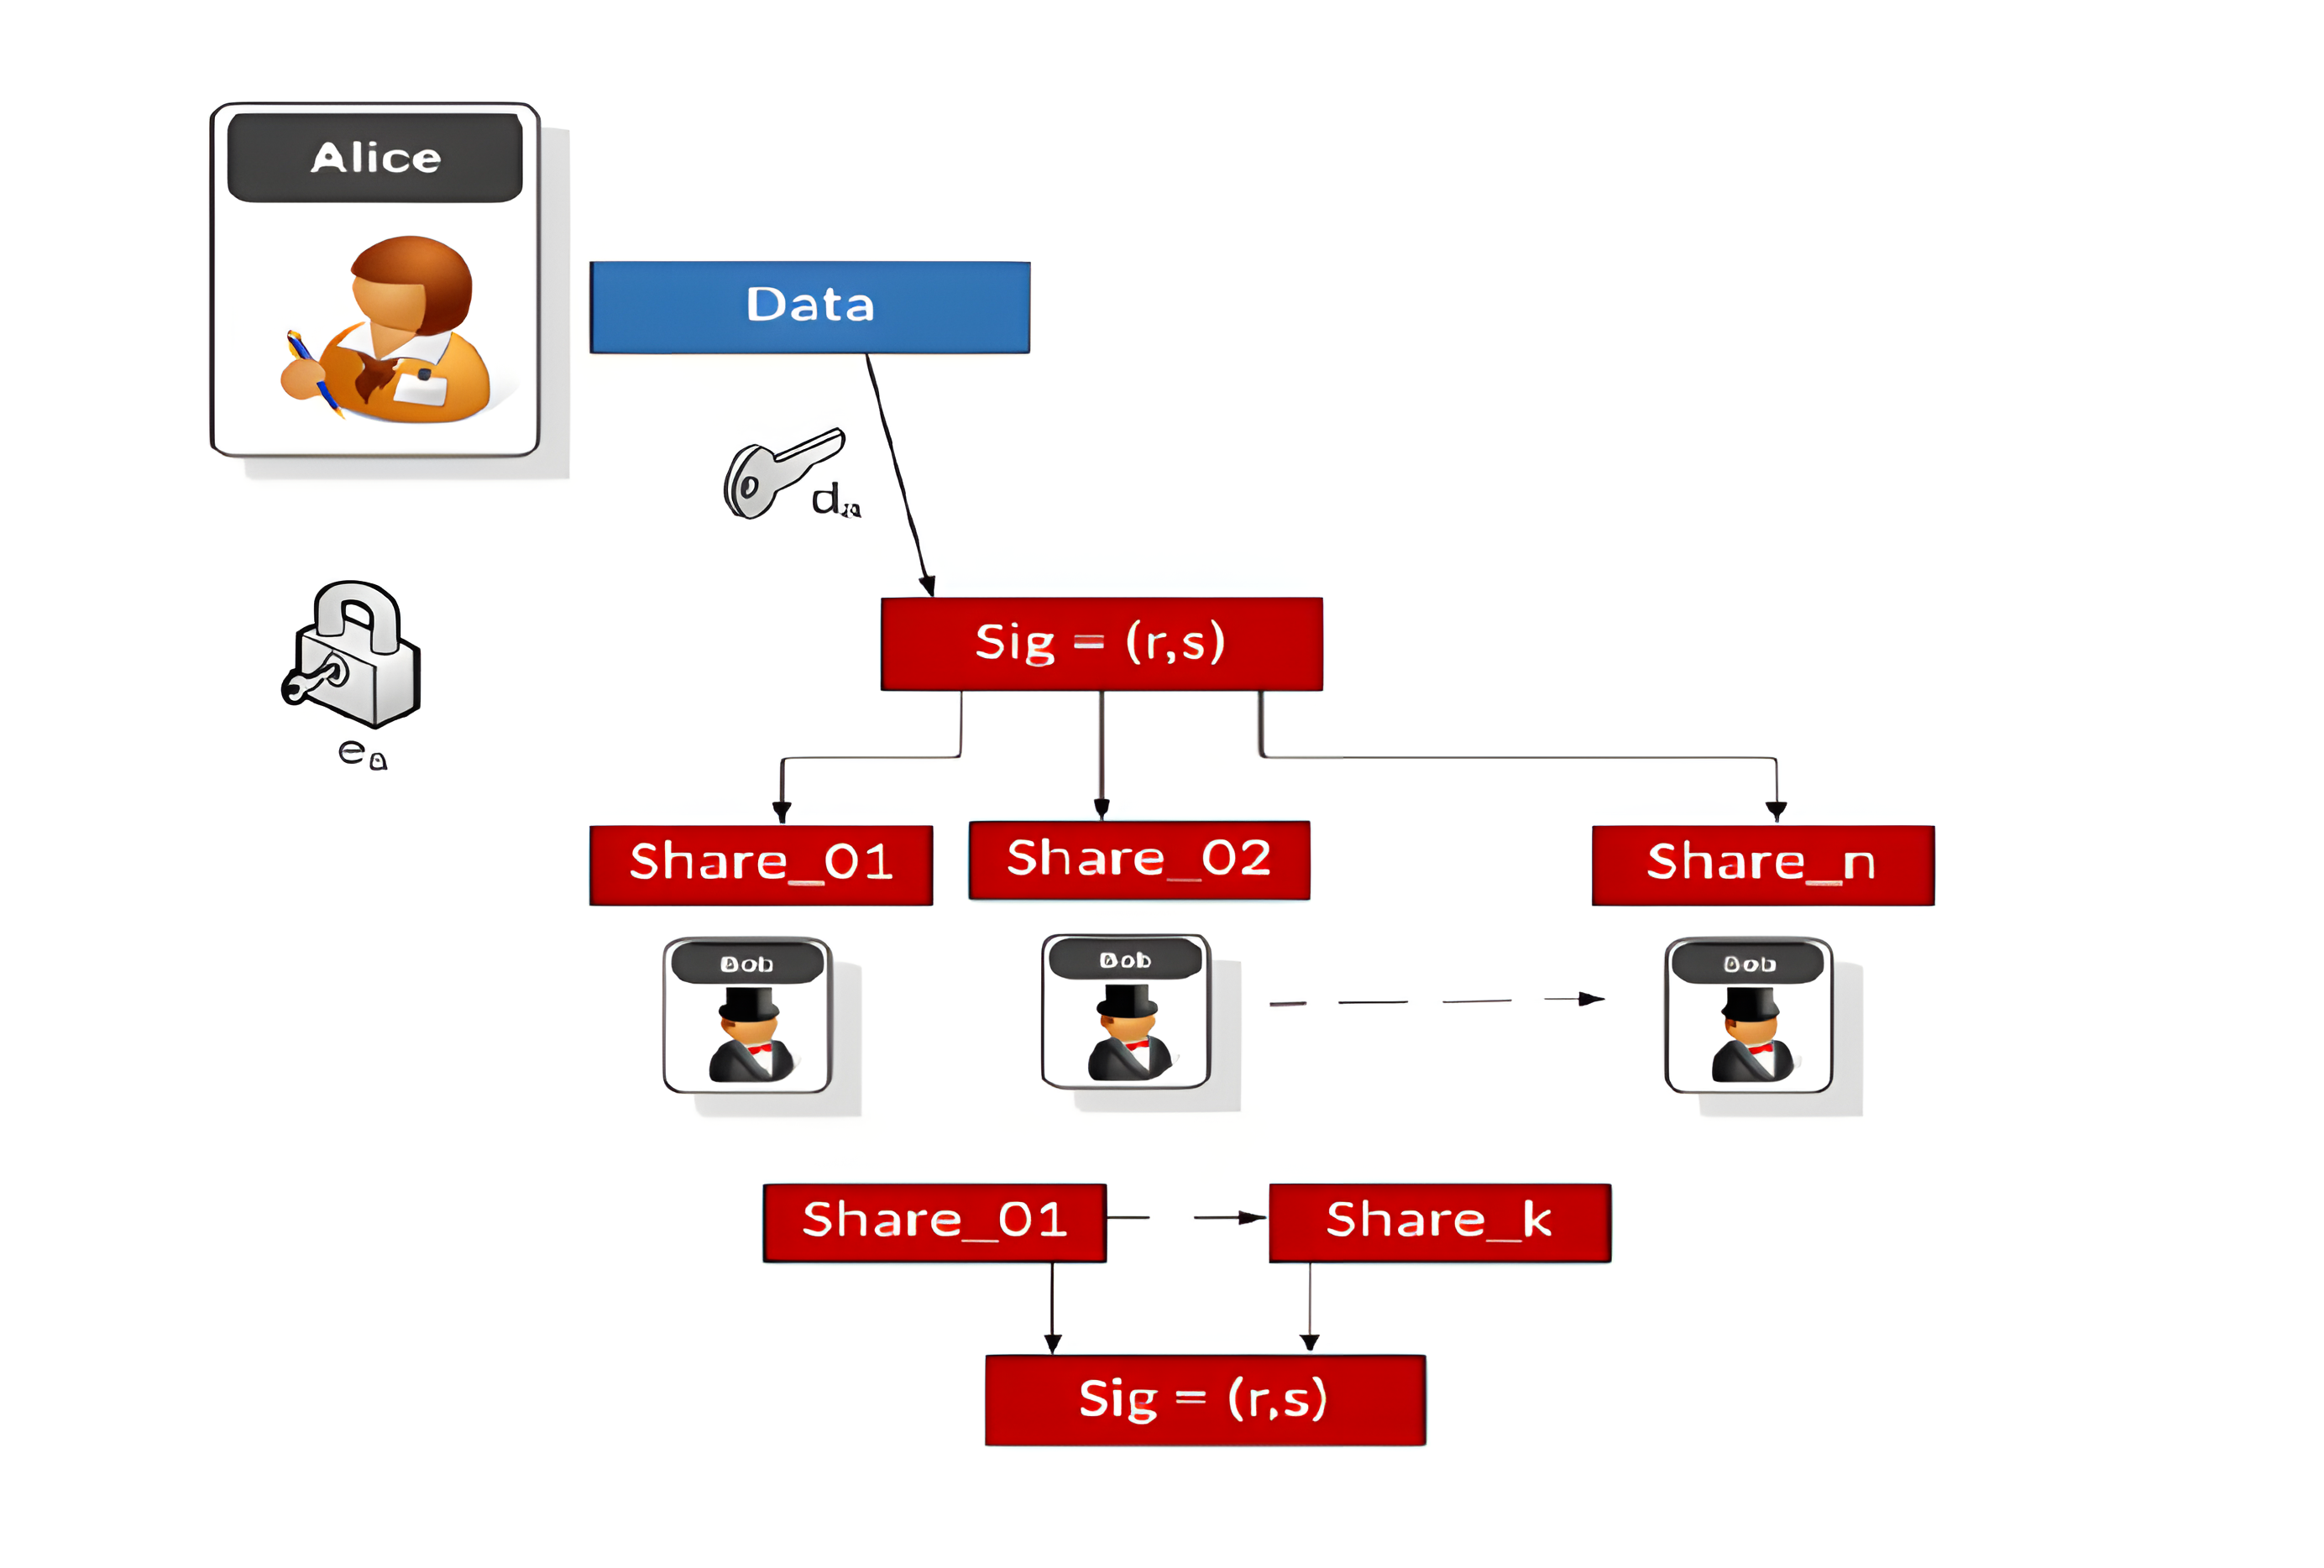
\includegraphics[width=0.9\columnwidth]{assets/images/ECDSA(1).png}
    \captionof{figure}{ECDSA}
\end{minipage}
  \end{center}
\vspace{-0.35em}

  \subsection*{\centering\uppercase{Quantum Threats to Classical Cryptography}}
  The primary motivation for post-quantum cryptography is the potential ability of quantum computers
  to break widely used cryptographic systems such as RSA and ECDSA. This threat is mainly based on
  Shor’s algorithm, which theoretically allows a sufficiently powerful quantum computer to solve
  integer factorization and discrete logarithm problems efficiently. Since RSA security depends on
  factoring large composite numbers and ECDSA depends on the elliptic curve discrete logarithm
  problem, both systems would become vulnerable if such quantum capability is achieved.

  \noindent
  In a real-world scenario, this means that a public key, which is openly shared during secure
  communication or stored on blockchain networks, could be used by an attacker to compute the
  corresponding private key. For example, in cryptocurrencies like Bitcoin, if a user’s public key is
  exposed, a powerful quantum computer could potentially derive the private key and authorize
  unauthorized transactions. Similarly, in internet security protocols such as HTTPS, intercepted
  communications that rely on classical public-key exchanges could be decrypted if private keys are
  recovered.

  \noindent
  Although current quantum computers are not capable of executing such attacks due to limitations in
  qubit stability and error correction, the theoretical risk remains significant. Google and the Dutch
  institute CWI officially broke the SHA-1 algorithm in 2017. They achieved this by producing a
  "collision"—where two entirely different files generate the same cryptographic fingerprint. It was
  broken using classical computing techniques not even quantum computers, this shows what powerful
  quantum computers can do to more powerful algorithms like HASH 160 and SHA256 which
  especially protects bitcoin wallets in future if not upgraded carefully. As a result SHA-1 is officially
  deprecated and is replaced by SHA-2 and SHA-3 for modern internet services.

  \noindent
  The transition to fault-tolerant quantum computers with a large number of logical qubits is still an
  open challenge, but once achieved, it could fundamentally change the security assumptions of modern
  cryptography.

  \subsection*{\centering\uppercase{Securing the Future: Quantum-Resistant Solutions}}
  To address the potential failure of RSA and ECDSA in a future where large-scale quantum computers
  exist, researchers have developed post-quantum cryptography (PQC), which focuses on cryptographic
  systems that remain secure even against quantum attacks. The key idea is to replace current schemes
  with alternatives that are not based on integer factorization or discrete logarithm problems, since these
  can be efficiently solved using Shor’s algorithm.

  \noindent
  One of the most promising approaches is lattice-based cryptography, which relies on hard problems in
  high-dimensional geometric structures called lattices. These problems, such as the Learning With
  Errors (LWE) problem, are believed to remain difficult even for quantum computers. Lattice-based
  schemes are currently considered the leading candidate for replacing both encryption and digital
  signature systems due to their balance of security and performance. Another important category is
  hash-based cryptography, which uses secure hash functions to build digital signatures that are highly
  resistant to quantum attacks, although they often come with larger signature sizes.

  \noindent
  Quantum cryptography emerging as another option, secures data transmission using the immutable
  laws of physics rather than complex mathematics that are currently in use in algorithms like
  RSA/ECDSA. Its primary application, \textbf{Quantum Key Distribution (QKD)}, utilizes particles of light
  (photons) to share encryption keys. Any attempt by an unauthorized third party to intercept or read
  the transmission alters the quantum state. This wave-function collapse instantly introduces
  detectable anomalies, exposing the eavesdropper governed by \textbf{Heisenberg Uncertainty Principle}.

  \noindent
  Code-based cryptography, such as systems derived from error-correcting codes, is another alternative
  that has shown strong resistance to both classical and quantum attacks, though it often suffers from
  large key sizes. These approaches are being actively evaluated and standardized by global research
  efforts, particularly those led by international security organizations.

  \begin{center}
\vspace{-0.5em}
\begin{minipage}{0.98\columnwidth}
\centering
    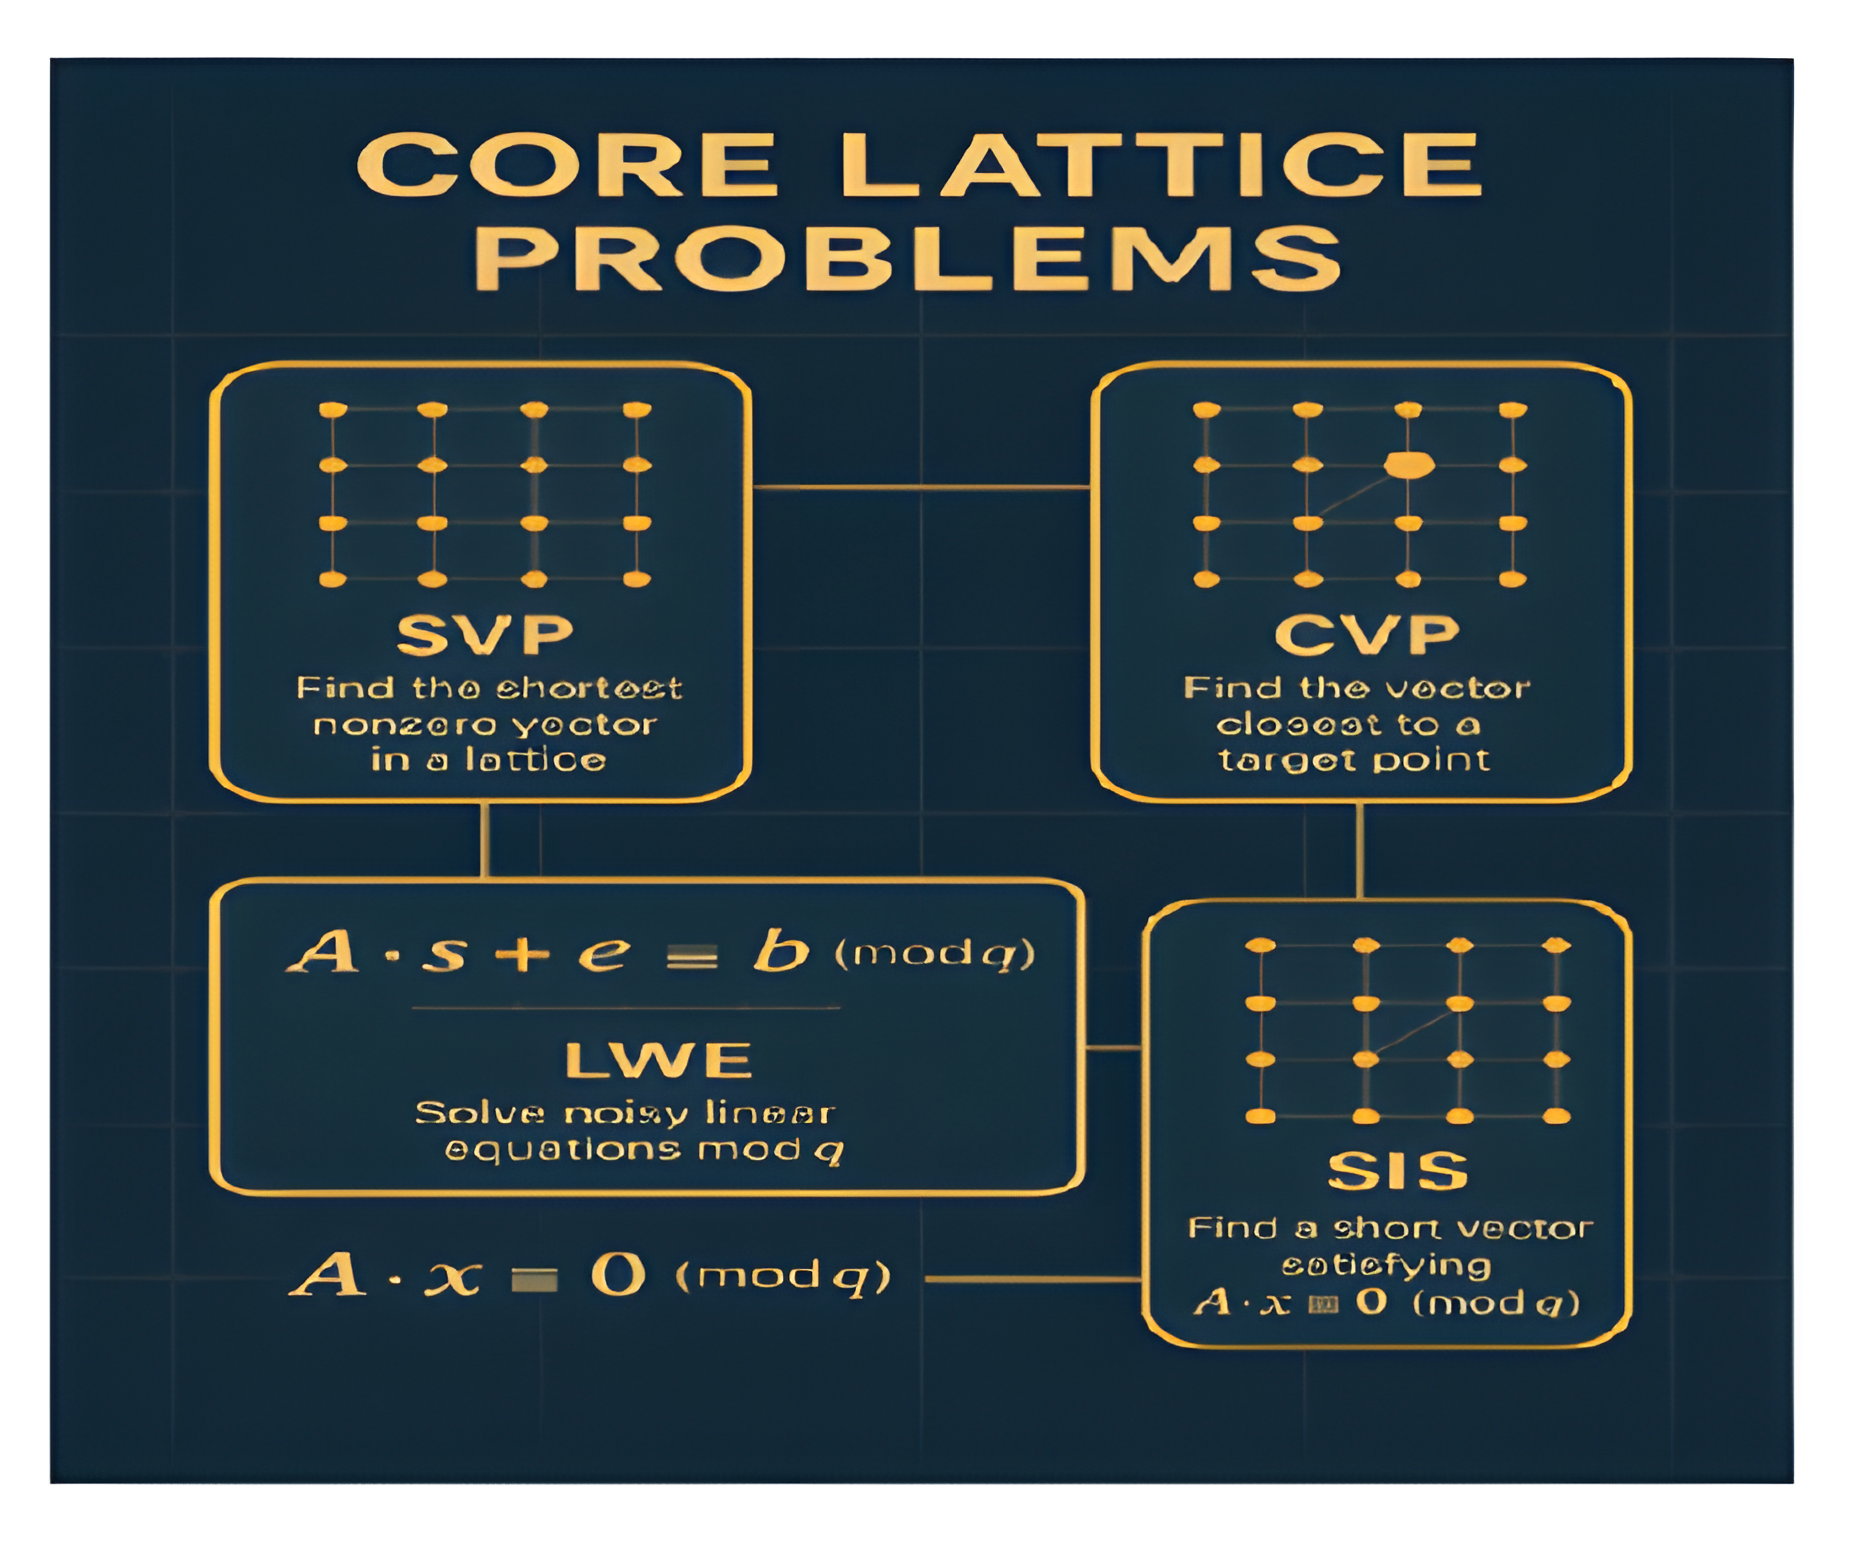
\includegraphics[width=0.6\columnwidth]{assets/images/CLP.png}
    \captionof{figure}{Core Lattice Problems}
\end{minipage}
  \end{center}
\vspace{-0.35em}

  \subsection*{\centering\uppercase{Standardization and Hybrid Cryptographic Transition}}
  To ensure a secure transition toward a quantum-safe future, global standardization efforts are being
  led by the National Institute of Standards and Technology (NIST), which has selected and
  recommended several post-quantum cryptographic algorithms for real-world deployment. Among
  these, CRYSTALS-Kyber has been chosen for key encapsulation mechanisms due to its strong
  security based on lattice problems and its relatively efficient performance compared to other
  candidates. Similarly, CRYSTALS-Dilithium has been selected for digital signatures, providing a
  practical replacement for RSA and ECDSA in many applications.

  \noindent
  In practice, the migration from classical to post-quantum cryptography is expected to follow a hybrid
  approach, where both traditional algorithms and post-quantum algorithms are used together. This
  hybrid cryptographic model ensures backward compatibility while gradually introducing quantum-
  resistant security. It allows systems to remain secure even if one of the underlying schemes is later
  found to be weaker than expected, thereby reducing migration risk.

  \noindent
  This transition phase is critical because global infrastructure, including secure communication
  protocols and blockchain systems, cannot be changed instantly. Therefore, hybrid cryptography
  provides a practical bridge between current security systems and fully post-quantum secure
  architectures.

  \subsection*{\centering\uppercase{Practical Constraints}}
  One of the practical responses to quantum-related security concerns is strengthening existing
  symmetric cryptographic and hashing systems rather than replacing them entirely. For example,
  algorithms such as SHA-256 can be upgraded to SHA-512 to increase the output size and
  computational resistance. While quantum algorithms like Grover’s algorithm can theoretically reduce
  the effective security strength of hash functions, increasing the hash size helps maintain a higher
  security margin even in a post-quantum environment. This approach is relatively simple because hash
  functions are not broken in the same fundamental way as RSA or ECDSA under quantum attacks.

  \noindent
  However, increasing security strength is not only about choosing larger algorithms, but also about
  balancing efficiency and system constraints. Larger hash outputs, such as those in SHA-512, increase
  computational overhead, storage requirements, and bandwidth usage, which may impact performance
  in large-scale systems like blockchain networks and distributed applications. This creates a trade-off
  between security level and practical efficiency.

  \noindent
  \textbf{The "Harvest Now, Decrypt Later" Threat:} Attackers are actively intercepting and storing
  encrypted data today to decrypt it later once quantum computers are viable. This pressures
  organizations to act now, even though PQC standards and browser trust store adoptions are still
  evolving.

  \noindent
  The main objective in post-quantum security design is therefore not only to maximize resistance
  against attacks, but to achieve strong security with minimal computational and storage cost. In other
  words, the goal is to improve security without significantly increasing sample size, key size, or system
  complexity. This balance is critical for real-world adoption, where millions of devices and systems
  must operate efficiently while still remaining secure against both classical and quantum threats.

  \subsection*{\centering\uppercase{Conclusion}}
  Post-quantum cryptography represents a necessary evolution of modern security systems in response
  to the theoretical capabilities of quantum computing. While RSA and ECDSA currently provide
  strong protection for digital communication, financial systems, and blockchain networks, their
  security is fundamentally based on mathematical assumptions that may not hold in a future quantum-
  enabled environment. The development of quantum algorithms such as Shor’s algorithm highlights
  that problems once considered computationally infeasible could become solvable, changing the
  foundation of trust in today’s digital infrastructure.

  \noindent
  In response to this potential risk, global efforts such as those led by NIST have introduced post-
  quantum standards, including CRYSTALS-Kyber for key encapsulation and CRYSTALS-Dilithium
  for digital signatures. Along with hybrid cryptographic approaches, these solutions aim to ensure a
  smooth transition from classical to quantum-resistant systems without disrupting existing
  infrastructure. However, the effectiveness of these solutions ultimately depends on how accurately
  future quantum capabilities are estimated and how quickly real-world systems can adapt.

  \noindent
  This leads to an important question: what if quantum computing reaches practical power sooner than
  expected? What if, one random day you open your eyes encrypted messages can be decrypted
  instantly, digital signatures can be forged, and cryptocurrency funds can disappear or be redirected
  without detection and authorization ? The uncertainty surrounding this possibility is precisely what
  makes post-quantum cryptography not just a theoretical study, but a critical requirement for the future
  of global digital security.

  \subsection*{\centering\uppercase{References}}
  \begin{justify}
  \Urlmuskip=0mu plus 1mu\relax
  \begin{enumerate}
    \item P. W. Shor, “Algorithms for quantum computation: Discrete logarithms and
      factoring,” Proceedings of the 35th Annual Symposium on Foundations of Computer
      Science, 1994.
    \item D. E. Shor, “Polynomial-time algorithms for prime factorization and discrete
      logarithms on a quantum computer,” SIAM Journal on Computing, vol. 26, no. 5,
      1997.
    \item National Institute of Standards and Technology (NIST), “Post-Quantum
      Cryptography Standardization Project,” 2024. \url{https://csrc.nist.gov/projects/post-quantum-cryptography}
      \item NIST, “FIPS 203: Module-Lattice-Based Key-Encapsulation Mechanism Standard
      (ML-KEM / CRYSTALS-Kyber),” 2024.
      \item \url{https://asecuritysite.com/ecdsa/ecdsa4}
      \item J. Buchmann, “Introduction to Cryptography,” Springer, 2017.
      \item D. J. Bernstein, “Post-quantum cryptography,” Communications of the ACM, vol. 61,
      no. 2, pp. 72--80, 2018.
  \end{enumerate}
  \end{justify}
\end{multicols}
% Full-width info box outside multicols
\begin{center}
  \begin{minipage}{\textwidth}
    \begin{tcolorbox}[
  colback=SoftYellow,
  colframe=IEEEblue!70!black,
  boxrule=0.5pt,
  arc=0mm,
  left=3mm, right=3mm, top=2.5mm, bottom=2.5mm
]
\small\RaggedRight \textbf{\color{IEEEblue!75!black}Did you know?} — \textbf{ECE Workbench:} \textbf{LTspice} simulates, \textbf{KiCad} draws PCB (run ERC/DRC), \textbf{PlatformIO} uploads, \textbf{MATLAB/Python} does FFT, \textbf{Git} tracks versions. \textit{Tip:} note units (\texttt{// 3.3V}) and commit often.
\end{tcolorbox}

  \end{minipage}
\end{center}

\begin{center}
  \section{\capitalisewords{Artificial Intelligence in Smart Healthcare Diagnosis Systems: Transforming Modern Medical Care}}
  Bushra Meraj, 3$^{rd}$ Year, ECE
\end{center}

\setcounter{figure}{0}

\begin{multicols}{2}
  \begin{abstract}
    \bfseries
    Artificial Intelligence (AI) has become an important technology in modern healthcare by improving the speed and accuracy of disease diagnosis. AI-based smart healthcare systems use technologies such as Machine Learning (ML), Deep Learning (DL), Natural Language Processing (NLP), and Computer Vision to analyse medical data, detect diseases, and assist doctors in clinical decision-making. These systems are widely used for diagnosing cancer, diabetes, heart diseases, and neurological disorders. AI also supports remote patient monitoring, personalized treatment, robotic surgery, and telemedicine services. Despite its numerous advantages, challenges such as data privacy, ethical concerns, algorithmic bias, and high implementation costs still exist. This report discusses the technologies, applications, advantages, challenges, recent developments, and case studies of AI in healthcare. It also provides a critical analysis of AI's role in improving healthcare while highlighting the importance of human supervision in medical decision-making.
  \end{abstract}
  \subsection*{\centering\uppercase{INTRODUCTION}}
  Healthcare is rapidly changing due to advances in Artificial Intelligence and digital technologies. Traditional diagnosis mainly depends on the knowledge and experience of doctors, which may sometimes lead to delays or human errors. AI helps overcome these limitations by analysing large amounts of medical data quickly and accurately.

  \noindent
  Artificial Intelligence refers to computer systems that can perform tasks such as learning, reasoning, and decision-making. In healthcare, AI analyses electronic health records, laboratory reports, medical images, and patient histories to assist doctors in identifying diseases at an early stage. Early diagnosis improves treatment success and reduces healthcare costs.

  \noindent
  The use of AI increased significantly after the COVID-19 pandemic, when hospitals adopted AI for disease detection, patient monitoring, and telemedicine. Today, AI is also being used in robotic surgery, wearable health devices, personalized medicine, and hospital management.

  \noindent
  Although AI provides many benefits, it cannot replace medical professionals. Doctors are still responsible for making final clinical decisions because patient care requires medical expertise, ethical judgment, and human empathy. Therefore, AI should be considered a decision-support tool rather than a substitute for healthcare professionals.

  \subsection*{\centering\uppercase{Objectives}}
  The objectives of this report are:
  \begin{itemize}
    \item To understand the role of Artificial Intelligence in healthcare.
    \item  To study the technologies used in smart healthcare diagnosis systems.
    \item  To explain the applications of AI in disease diagnosis.
    \item  To analyse the advantages and limitations of AI in healthcare.
    \item  To discuss recent developments and real-life case studies.
    \item  To examine the future scope of AI in modern healthcare systems.

  \end{itemize}

  \subsection*{\centering\uppercase{Technologies Used in Smart Healthcare Diagnosis Systems}}
  Smart healthcare diagnosis systems use various Artificial Intelligence technologies to analyse medical data and assist healthcare professionals in making accurate decisions. The major technologies are explained below.

  \subsubsection*{Machine Learning (ML)}
  Machine Learning is a branch of AI that enables computers to learn from data without being explicitly programmed. ML algorithms analyse patient records, laboratory reports, and medical histories to identify disease patterns and predict health conditions.

  \noindent
  Common machine learning techniques include:
  \begin{itemize}
    \item Supervised Learning
    \item Unsupervised Learning
    \item Reinforcement Learning
  \end{itemize}

  Machine Learning is widely used for predicting diseases such as diabetes, heart disease, and cancer. Studies have shown that ML models can achieve diagnostic accuracies of over 90\% for several chronic diseases when trained using high-quality medical datasets. However, their performance depends on the availability of accurate and unbiased data.

  \subsubsection*{Deep Learning (DL)}
  Deep Learning is an advanced form of Machine Learning that uses artificial neural networks with multiple layers to process complex medical data. It is particularly effective in analysing medical images.

  \noindent
  Applications include:
  \begin{itemize}
    \item Detection of breast cancer from mammograms
    \item Identification of pneumonia from chest X-rays
    \item Brain tumour detection using MRI scans
    \item Skin cancer classification
  \end{itemize}

  Deep learning significantly reduces the workload of radiologists by providing faster image analysis. However, these models often require large datasets and powerful computing resources, making them expensive to develop and maintain.

  \subsubsection*{Natural Language Processing (NLP)}
  Natural Language Processing enables computers to understand and analyse human language. In healthcare, NLP processes clinical notes, electronic health records (EHRs), prescriptions, and research articles.

  \noindent
  Its applications include:
  \begin{itemize}
    \item Automatic clinical documentation
    \item Medical report summarization
    \item Extraction of patient information
    \item Voice-assisted healthcare systems
  \end{itemize}

  NLP reduces administrative work for healthcare professionals and improves the management of patient records.

  \subsubsection*{Computer Vision}
  Computer Vision allows AI systems to interpret medical images such as X-rays, CT scans, MRI scans, and ultrasound images. It helps doctors identify abnormalities quickly and accurately.

  \noindent
  Major applications include:
  \begin{itemize}
    \item Tumour detection
    \item Fracture identification
    \item Organ segmentation
    \item Disease progression monitoring
  \end{itemize}

  Computer Vision has improved diagnostic accuracy in radiology and pathology. However, image quality and dataset diversity directly affect system performance.

  \subsubsection*{Internet of Medical Things (IoMT)}
  The Internet of Medical Things (IoMT) consists of connected medical devices that continuously collect and transmit patient health data.

  \noindent
  Examples include:
  \begin{itemize}
    \item Smartwatches
    \item Heart-rate monitors
    \item Blood glucose monitors
    \item Smart blood pressure devices
  \end{itemize}

  These devices support remote patient monitoring, enabling doctors to detect health problems early and reduce unnecessary hospital visits.

  \subsubsection*{Critical Analysis}
  Each AI technology offers unique advantages, but no single technology is sufficient for all healthcare applications. Machine Learning performs well with structured medical data, while Deep Learning is more suitable for medical imaging. NLP is effective for analysing text-based records, whereas Computer Vision excels in image interpretation. Integrating these technologies into a single healthcare system provides more reliable and accurate diagnostic support. Nevertheless, challenges such as data privacy, algorithmic bias, and high implementation costs must be addressed before AI can be widely adopted in all healthcare settings.

  \subsection*{\centering\uppercase{Applications of AI in Smart Healthcare Diagnosis Systems}}
  Artificial Intelligence is transforming healthcare by improving the accuracy, speed, and efficiency of medical diagnosis. Some of its major applications are discussed below.

  \subsubsection*{Disease Diagnosis}
  AI systems help doctors identify diseases by analysing symptoms, medical records, laboratory reports, and diagnostic images. They are widely used for detecting diseases such as breast cancer, diabetes, heart disease, Alzheimer's disease, and lung disorders. Early diagnosis enables timely treatment and improves patient survival rates.

  \noindent
  Recent studies have shown that AI-assisted diagnosis can achieve an accuracy of over 90\% for several diseases when trained on high-quality datasets. However, doctors must always verify AI predictions before making final clinical decisions.

  \subsubsection*{Medical Imaging Analysis}
  Medical imaging is one of the most successful applications of AI. Deep learning algorithms analyse X-rays, CT scans, MRI scans, and ultrasound images to detect abnormalities that may not be easily visible to the human eye.

  \noindent
  Benefits include:
  \begin{itemize}
    \item Faster image analysis
    \item Improved diagnostic accuracy
    \item Reduced workload for radiologists
    \item Early detection of diseases
  \end{itemize}

  AI-assisted imaging has significantly improved the diagnosis of cancer, brain tumours, fractures, and lung infections.

  \subsubsection*{Personalized Medicine}
  {\justifying
  AI supports personalized medicine by analysing a patient's genetic information, medical history, lifestyle, and previous treatments. Based on this information, it recommends treatment plans that are more suitable for individual patients.
  \par}

  \noindent
  Advantages include:
  \begin{itemize}
    \item Better treatment selection
    \item Reduced side effects
    \item Improved patient outcomes
    \item More effective long-term disease management
  \end{itemize}

  This approach is especially useful in cancer treatment and chronic disease management.

  \subsubsection*{Remote Patient Monitoring}
  Wearable devices and smart sensors continuously monitor patients' health conditions and transmit data to healthcare providers. AI analyses this data to detect abnormal changes and alert doctors when necessary.

  \noindent
  Applications include:
  \begin{itemize}
    \item Heart rate monitoring
    \item Blood glucose monitoring
    \item Blood pressure monitoring
    \item Oxygen saturation monitoring
  \end{itemize}

  Remote monitoring became increasingly important during the COVID-19 pandemic by reducing unnecessary hospital visits while ensuring continuous patient care.

  \subsubsection*{Robotic Surgery}
  AI-powered robotic systems assist surgeons in performing complex and minimally invasive procedures with greater precision. These systems improve surgical accuracy and reduce the risk of complications.

  \noindent
  Benefits include:
  \begin{itemize}
    \item Smaller surgical incisions
    \item Reduced blood loss
    \item Faster recovery
    \item Shorter hospital stays
  \end{itemize}
  Although robotic systems improve surgical performance, they are expensive and still require experienced surgeons for operation and supervision.

  \subsubsection*{Robotic Surgery}
  AI-powered virtual assistants and healthcare chatbots provide basic medical guidance and support to patients. They help reduce the workload of healthcare professionals by handling routine tasks.

  \noindent
  Common functions include:
  \begin{itemize}
    \item Appointment scheduling
    \item Medication reminders
    \item Symptom checking
    \item Providing health information
    \item Answering patient queries
  \end{itemize}
  These systems improve healthcare accessibility, particularly for patients living in remote areas.

  \subsubsection*{Critical Analysis}
  AI applications have significantly improved the quality and efficiency of healthcare services. However, AI should not be considered a replacement for doctors. Incorrect predictions may occur due to poor-quality data, biased algorithms, or rare medical conditions. Therefore, AI should function as a clinical decision-support system while final diagnosis and treatment decisions remain the responsibility of qualified healthcare professionals.

  \subsection*{\centering\uppercase{Advantages and Challenges of AI in Smart Healthcare Diagnosis Systems}}
  Artificial Intelligence offers numerous benefits to the healthcare industry, but its implementation also presents several technical, ethical, and financial challenges. Understanding both aspects is essential for the responsible use of AI in medical diagnosis.

  \subsubsection*{Advantages of AI in Healthcare}
\begin{enumerate}[label=\alph*)]
  \item \textbf{Improved Diagnostic Accuracy:} AI systems can analyse large volumes of medical data and identify disease patterns that may be difficult for humans to detect. This helps doctors diagnose diseases such as cancer, heart disease, and diabetes more accurately and at an earlier stage. Research has shown that AI-assisted medical imaging can achieve diagnostic accuracy of over 90\% for certain conditions.
  \item \textbf{Faster Diagnosis:} AI processes medical images, laboratory reports, and patient records within seconds, reducing the time required for diagnosis. Faster diagnosis allows patients to receive timely treatment, especially in emergency situations such as stroke or heart attack.
  \item \textbf{Personalized Treatment:} AI analyses a patient's medical history, genetic information, and lifestyle to recommend personalized treatment plans. This improves treatment effectiveness and reduces the risk of adverse drug reactions.
  \item \textbf{Cost Reduction:} Automation of administrative tasks, medical documentation, and diagnostic procedures reduces operational costs for hospitals. AI also minimizes unnecessary medical tests, making healthcare more affordable for patients.
  \item \textbf{Better Patient Monitoring:} Wearable devices connected to AI systems continuously monitor patients' vital signs, including heart rate, blood pressure, and blood glucose levels. Doctors receive real-time alerts if any abnormal changes are detected, improving the management of chronic diseases.
\end{enumerate}

\subsubsection*{Challenges and Limitations}

\begin{enumerate}[label=\alph*)]
\item \textbf{Data Privacy and Security:} Healthcare data contains sensitive patient information. If AI systems are not properly secured, they may become vulnerable to cyberattacks and data breaches. Strong encryption and strict access control are necessary to protect patient privacy.
\item \textbf{Algorithmic Bias:} AI systems learn from historical data. If the training data is incomplete or biased, the AI model may produce inaccurate or unfair results for certain patient groups. Regular testing and diverse datasets are required to reduce bias.
\item \textbf{High Implementation Cost:} Developing AI-based healthcare systems requires advanced hardware, specialized software, and skilled professionals. These high costs make AI adoption difficult for many small hospitals and healthcare centres.
\item \textbf{Ethical and Legal Issues:} Questions regarding patient consent, accountability, and legal responsibility remain major concerns. If an AI system makes an incorrect diagnosis, determining who is responsible—the developer, hospital, or doctor—can be challenging.
\end{enumerate}

\subsubsection*{Critical Analysis}
Artificial Intelligence has significantly improved healthcare by increasing diagnostic accuracy, reducing workload, and supporting faster clinical decisions. However, AI should not be viewed as a replacement for healthcare professionals. Medical decisions often require clinical experience, ethical judgment, and empathy, which AI cannot provide. The most effective approach is \textbf{human-AI collaboration}, where AI supports doctors by providing accurate analysis while final decisions remain with qualified medical professionals.

\noindent
For successful implementation, healthcare organizations should invest in secure data management, high-quality datasets, regular model evaluation, and proper training of healthcare staff. Responsible use of AI will ensure that its benefits outweigh its limitations and contribute to safer and more efficient healthcare services.

\subsection*{\centering\uppercase{Recent Developments and Case Studies}}
\subsubsection*{Recent Developments in AI Healthcare (2023-2026)}
Artificial Intelligence has continued to evolve rapidly in recent years, making healthcare systems more efficient and patient-centred. Several new technologies are improving the quality of diagnosis and treatment.

\noindent
\textbf{Generative AI in Healthcare:} Hospitals are beginning to use Generative AI to prepare medical reports, summarize patient records, and assist doctors in clinical documentation. This reduces paperwork and allows healthcare professionals to spend more time with patients.

\noindent
\textbf{Explainable AI (XAI):} One limitation of traditional AI models is that they often do not explain how a decision is made. Explainable AI helps doctors understand the reasoning behind AI predictions, increasing trust and supporting better clinical decisions.

\noindent
\textbf{AI in Drug Discovery:} Pharmaceutical companies now use AI to identify potential drug candidates much faster than traditional methods. This reduces research time and lowers development costs.

\noindent
\textbf{Smart Wearable Devices:}
Modern smartwatches and wearable sensors continuously monitor heart rate, blood pressure, oxygen levels, and sleep patterns. AI analyses this data in real time and alerts doctors if abnormal health conditions are detected.

\noindent
These developments show that AI is expanding beyond disease diagnosis to become an important part of preventive healthcare and hospital management.

\subsubsection*{Case Studies}
\textbf{Case Study 1:} Google DeepMind and Eye Disease Detection
Google DeepMind developed an AI system capable of analysing retinal scans to detect more than 50 eye diseases. The system provides fast and accurate diagnosis, helping ophthalmologists identify serious eye conditions at an early stage. Early detection improves the chances of successful treatment and reduces the risk of vision loss.

\noindent
\textbf{Case Study 2:} AI During the COVID-19 Pandemic
During the COVID-19 pandemic, AI was widely used to analyse chest X-rays and CT scans, predict disease spread, support vaccine research, and monitor infected patients. AI-based systems helped hospitals manage resources efficiently during periods of high patient demand.

\noindent
\textbf{Case Study 3:} AI in Cancer Detection
Deep learning algorithms are now used to analyse mammograms and pathology images for breast cancer detection. These systems assist radiologists by identifying suspicious areas that require further examination, leading to earlier diagnosis and improved treatment outcomes.

\noindent
\textbf{Case Study 4:} AI in Cardiology
AI-powered software analyses Electrocardiogram (ECG) data to identify abnormal heart rhythms and predict cardiovascular diseases. Early identification enables doctors to begin treatment sooner, reducing the risk of severe cardiac complications.

\noindent
\textbf{Case Study 5:} AI-Assisted Robotic Surgery
Hospitals around the world use AI-assisted robotic surgical systems to perform minimally invasive procedures. These systems provide greater precision, reduce blood loss, shorten recovery time, and lower the risk of surgical complications. However, they still require experienced surgeons to supervise every procedure.

\subsubsection*{Critical Analysis}
The above case studies demonstrate that AI has significantly improved disease diagnosis, medical imaging, and patient monitoring. However, successful implementation depends on high-quality data, skilled healthcare professionals, and proper regulatory oversight. AI systems should always support medical experts rather than replace them. Combining human expertise with AI technology provides the most reliable and effective healthcare outcomes.

\subsection*{\centering\uppercase{Future Scope}}
Artificial Intelligence is expected to play an even greater role in healthcare in the coming years. Continuous improvements in computing power, cloud technology, and medical data analysis will make AI systems more accurate, efficient, and affordable.

\noindent
Some important future developments include:
\begin{itemize}
\item AI-assisted early detection of diseases before symptoms appear.
\item Faster drug discovery and development using AI algorithms.
\item Wider use of robotic surgery for complex medical procedures.
\item Expansion of telemedicine and remote patient monitoring.
\item Smart hospitals with integrated AI systems for patient management.
\item Better use of wearable devices for continuous health monitoring.
\item Explainable AI (XAI) to improve transparency and build trust among doctors and patients.
\end{itemize}
Governments and healthcare organizations are also developing regulations to ensure that AI systems are safe, reliable, and ethically used. With proper implementation, AI has the potential to improve healthcare accessibility and quality, particularly in rural and underserved areas.

\subsection*{\centering\uppercase{Conclusion}}
Artificial Intelligence has become a powerful technology that is transforming modern healthcare diagnosis systems. By using Machine Learning, Deep Learning, Natural Language Processing, and Computer Vision, AI helps healthcare professionals diagnose diseases more accurately and efficiently. It also supports medical imaging, personalized medicine, remote patient monitoring, robotic surgery, and virtual healthcare services.

\noindent
The report has shown that AI offers several advantages, including improved diagnostic accuracy, faster decision-making, reduced healthcare costs, and better patient care. Real-world case studies demonstrate that AI has already made significant contributions in areas such as cancer detection, cardiology, eye disease diagnosis, and pandemic management.

\noindent
However, AI also faces important challenges, including data privacy, cybersecurity, algorithmic bias, ethical concerns, and high implementation costs. These issues must be carefully addressed to ensure responsible and fair use of AI in healthcare.

\noindent
In conclusion, Artificial Intelligence should be viewed as a tool that supports healthcare professionals rather than replacing them. A combination of human expertise and intelligent AI systems can improve the quality of healthcare services and patient outcomes. With continuous technological advancements and proper regulations, AI is expected to play an increasingly important role in building smarter, safer, and more accessible healthcare systems in the future.

\subsection*{\centering\uppercase{References}}
{\small
\begin{justify}
\begin{enumerate}[
  label={[\arabic*]},
  leftmargin=*,
  labelsep=0.5em,
  itemsep=0.20em,
  parsep=0pt,
  topsep=0.15em
]
  \item J. Jiang et al., "Artificial Intelligence in Healthcare: Past, Present and Future," Stroke and Vascular Neurology, vol. 2, no. 4, pp. 230--243, 2017.
  \item E. J. Topol, Deep Medicine: How Artificial Intelligence Can Make Healthcare Human Again. New York, NY, USA: Basic Books, 2019.
  \item S. Yu and M. Kohane, "Framing the Challenges of Artificial Intelligence in Medicine," BMJ Quality \& Safety, vol. 28, no. 3, pp. 238--241, 2019.
  \item A. Esteva et al., "Dermatologist-Level Classification of Skin Cancer with Deep Neural Networks," Nature, vol. 542, no. 7639, pp. 115--118, 2017.
  \item P. Hamet and J. Tremblay, "Artificial Intelligence in Medicine," Metabolism, vol. 69, pp. S36--S40, 2017.
  \item R. Miotto et al., "Deep Learning for Healthcare: Review, Opportunities and Challenges," Briefings in Bioinformatics, vol. 19, no. 6, pp. 1236--1246, 2018.
  \item World Health Organization, Ethics and Governance of Artificial Intelligence for Health. Geneva, Switzerland: WHO, 2021.
  \item R. Davenport and R. Kalakota, "The Potential for Artificial Intelligence in Healthcare," Future Healthcare Journal, vol. 6, no. 2, pp. 94--98, 2019.
  \item D. Shen, G. Wu, and H.-I. Suk, "Deep Learning in Medical Image Analysis," Annual Review of Biomedical Engineering, vol. 19, pp. 221--248, 2017.
  \item K. He et al., "Deep Residual Learning for Image Recognition," Proceedings of the IEEE Conference on Computer Vision and Pattern Recognition (CVPR), pp. 770--778, 2016.
  \item World Health Organization, "Regulatory Considerations on Artificial Intelligence for Health," WHO Technical Report, 2023.
  \item U.S. Food and Drug Administration (FDA), Artificial Intelligence and Machine Learning (AI/ML)-Enabled Medical Devices, 2024.
  \item M. Bohr and K. Memarzadeh, Artificial Intelligence in Healthcare. Academic Press, 2020.
  \item S. Rajpurkar et al., "Deep Learning for Chest Radiograph Diagnosis: CheXNet," Stanford University Research Report, 2017.
  \item J. Lee, Y. Kim, and H. Park, "Recent Advances in Artificial Intelligence for Smart Healthcare Systems," IEEE Access, vol. 12, pp. 12543--12560, 2024.
\end{enumerate}
\end{justify}
}


\end{multicols}

\begin{center}
\begin{tcolorbox}[colback=SoftBlue, colframe=IEEEblue!70!black, boxrule=0.5pt, arc=0mm, left=3mm, right=3mm, top=2mm, bottom=2mm, width=0.92\textwidth]
\small\RaggedRight \textbf{\color{IEEEblue!75!black}Did you know?} — AI has matched dermatologists on dermoscopy, with deep nets reaching $>$90\% accuracy for skin-cancer classification.
\end{tcolorbox}
\end{center}

\begin{center}
  \section{\capitalisewords{From Neurons to Silicon: The Neuromorphic Revolution}}
  Tiyasa Pal, 3$^{rd}$ Year, ECE
\end{center}

\setcounter{figure}{0}
\setcounter{table}{0}

\begin{multicols}{2}
  \begin{abstract}
    \bfseries
    Neuromorphic computing is an interdisciplinary hardware discipline that implements brain-inspired principles -co-located memory and computation, event-driven (spike-based) signalling, and adaptive synaptic weighting -directly in silicon, in contrast to the instruction-driven, memory-separated Von Neumann model that underlies conventional CPUs and GPUs. This report examines the architectural principles of neuromorphic systems, benchmarks representative chips quantitatively, and critically evaluates the gap between demonstrated laboratory efficiency and real-world commercial deployment.

    \noindent
    Published results indicate that the approach can deliver large efficiency gains on workloads that map naturally onto sparse, event-driven computation: IBM's NorthPole reports roughly 25× higher energy efficiency (frames-per-second per watt) than a comparable 12 nm-class GPU on the ResNet-50 image-classification benchmark, while Intel's Hala Point system (1,152 Loihi 2 chips, 1.15 billion neurons, 128 billion synapses) sustains approximately 20 petaops at over 15 trillion 8-bit operations per second per watt. Earlier devices - IBM TrueNorth (1 million neurons, 256 million synapses, 28 nm) and Intel's first-generation Loihi (131,072 neurons, 130 million synapses, 14 nm) - established the feasibility of large-scale spiking hardware but were confined to research settings.

    \noindent
    However, these efficiency figures are workload-specific rather than general-purpose: dense-matrix operations that dominate contemporary AI, such as transformer-based language models, do not map efficiently onto spiking substrates, and the absence of a mature, standardized programming model (comparable to CUDA for GPUs) remains the principal barrier to commercial adoption. This report therefore combines a technical description of neuromorphic architecture with a critical assessment of where the technology currently delivers genuine advantage, where its benefits are overstated, and what would be required for wider adoption.
  \end{abstract}

  \subsection*{\centering\uppercase{INTRODUCTION}}
  The rapid advancement of artificial intelligence and machine learning has increased the demand for faster and more efficient computing systems. Conventional computers are mainly based on the Von Neumann architecture, where memory and processing units are separated. Although this architecture has been highly successful for decades, it suffers from limitations such as high-power consumption, memory bottlenecks, and reduced efficiency in handling complex AI tasks.

  \noindent
  The human brain, by contrast, is an extremely efficient biological computing system. It contains nearly 86 billion neurons connected through trillions of synapses, enabling massive parallel processing while consuming only about 20 watts of power. Inspired by this efficiency, scientists and engineers developed the concept of neuromorphic computing, which imitates the neural structure and operation of the brain to build intelligent machines capable of learning, adaptation, and decision-making.

  \noindent
  Neuromorphic chips are specifically designed hardware systems that mimic biological neural networks. These chips use artificial neurons and synapses to process information through spikes, similar to the way neurons communicate in the human brain. Unlike traditional processors that perform sequential computation, neuromorphic chips support parallel and event-driven processing, making them well suited to specific classes of AI workloads. Today, neuromorphic computing is explored in robotics, autonomous vehicles, healthcare, cybersecurity, and edge devices, although - as this report will show- the technology remains largely confined to research and specialised deployments rather than mainstream commercial computing.

  \subsection*{\uppercase{Core Concept and Analysis}}
  \subsubsection*{Biological Inspiration: Structure of the Human Brain}
  The foundation of neuromorphic computing lies in neuroscience. The human brain is a massively parallel and energy-efficient processing system.

  \begin{enumerate}
    \item \textbf{Neurons:} Neurons are the fundamental units of the brain. Each neuron receives signals from other neurons through dendrites, processes the information in the cell body (soma), and transmits output through the axon.
    \item \textbf{Synapses:} Synapses are the connection points between neurons. They determine the strength of communication between neurons. Learning in the brain occurs through changes in synaptic strength.
    \item \textbf{Action Potentials (Spikes):} Neurons communicate using electrical impulses called spikes or action potentials. A neuron fires only when its membrane potential exceeds a certain threshold.
    \item Key Characteristics of the Brain:
      \begin{itemize}
        \item Massive parallel processing
        \item Event-driven computation (neurons activate only when needed)
        \item Adaptive learning through synaptic plasticity
        \item Fault tolerance (the brain continues functioning even with damaged neurons)
        \item Extremely low energy consumption
      \end{itemize}
  \end{enumerate}
  These characteristics form the conceptual blueprint for neuromorphic systems.

  \begin{center}
\vspace{-0.5em}
\begin{minipage}{0.98\columnwidth}
\centering
    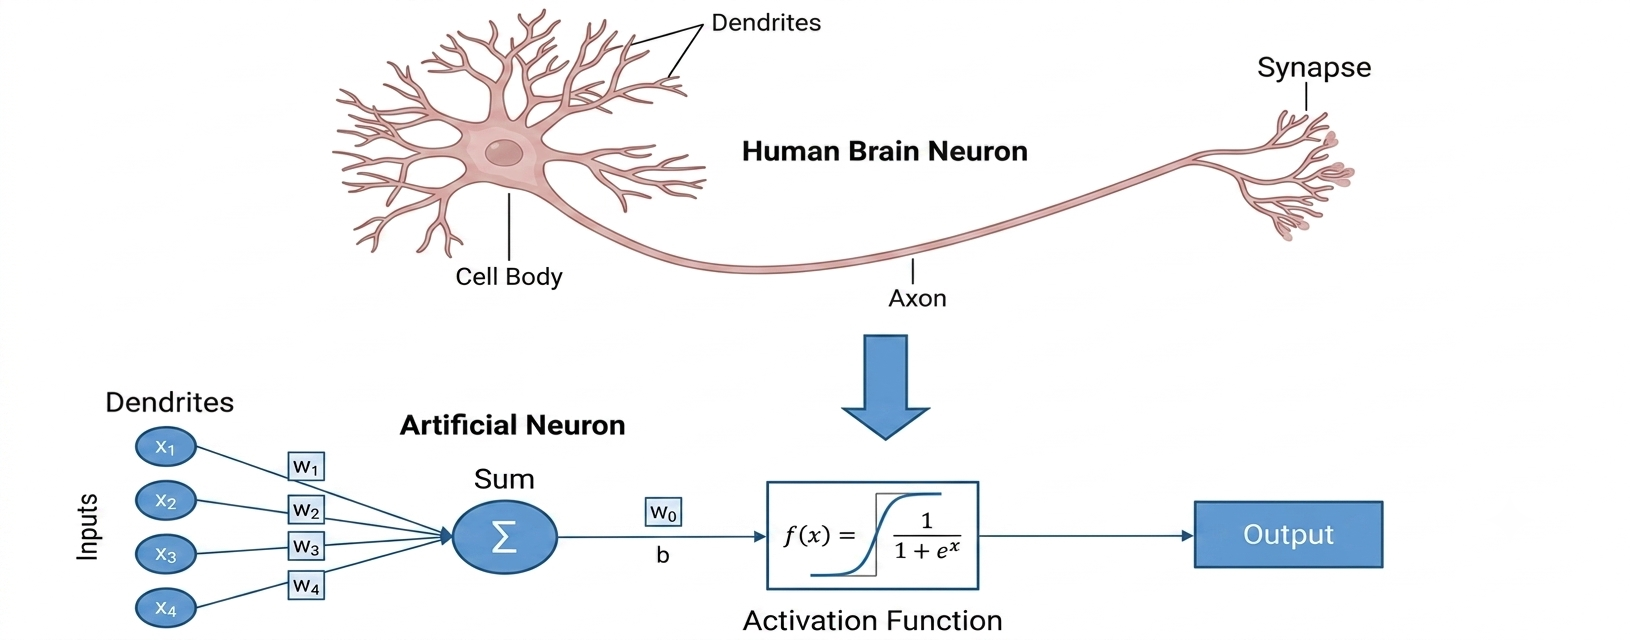
\includegraphics[width=0.85\columnwidth]{assets/images/neuron.png}
    \captionof{figure}{Schematic comparison of a biological neuron and an artificial neuron (dendrites, soma, axon, and synapse mapped to inputs, weighted sum, activation function, and output). Diagram prepared by the author to illustrate the structural analogy described by Mead [1] and Maass [2].}
\end{minipage}
  \end{center}
\vspace{-0.35em}

  \subsubsection*{Evolution from Von Neumann Architecture to Neuromorphic Design}
  Traditional computing systems follow the Von Neumann architecture, in which the CPU performs computation, memory stores data separately, and data transfer between the two creates bottlenecks — the well-known “Von Neumann bottleneck.” Neuromorphic architecture addresses this by integrating memory and computation within the same processing units, similar to synapses in the brain.

  Table~1 compares Von Neumann and neuromorphic systems.

\begin{center}
\vspace{-0.5em}
\begin{minipage}{0.98\columnwidth}
\centering
    \captionof{table}{Comparison between Von Neumann and Neuromorphic systems (adapted from principles discussed in Indiveri \& Liu [3]).}
    \setlength{\tabcolsep}{3pt}
    \renewcommand{\arraystretch}{1.3}
    \begin{tabular}{@{}>{\RaggedRight\arraybackslash}p{0.25\columnwidth}
        >{\RaggedRight\arraybackslash}p{0.26\columnwidth}
      >{\RaggedRight\arraybackslash}p{0.37\columnwidth}@{}}
      \toprule
      \textbf{Feature} & \textbf{Von Neumann Systems} & \textbf{Neuromorphic Systems} \\
      \midrule
      Processing  & Sequential & Parallel \\
      Memory      & Separate & Integrated \\
      Power Usage & High & Very Low \\
      Operation   & Clock-driven & Event-driven \\
      \bottomrule
    \end{tabular}
\end{minipage}
  \end{center}

  \begin{center}
\vspace{-0.5em}
\begin{minipage}{0.98\columnwidth}
\centering
    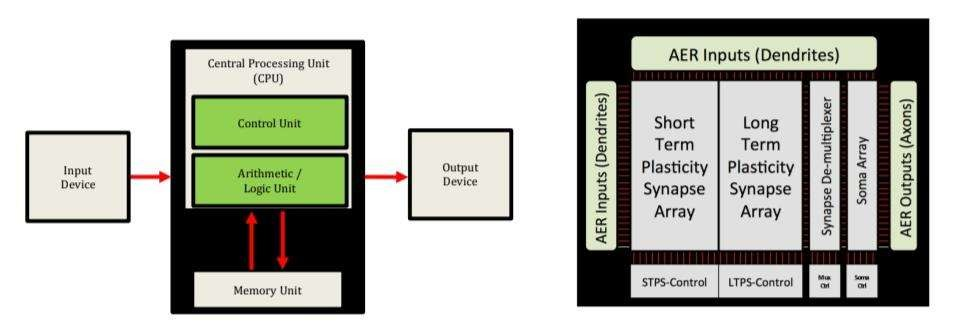
\includegraphics[width=0.85\columnwidth]{assets/images/Von Neuman system.jpg}
    \captionof{figure}{Block-level comparison of a conventional Von Neumann CPU (separated control unit, ALU, and memory) with a neuromorphic core (integrated plasticity, synapse array, and soma array addressed via AER). Diagram prepared by the author, conceptually based on Indiveri \& Liu [3] and Davies et al. [6].}
\end{minipage}
  \end{center}
\vspace{-0.35em}

  \subsubsection*{Spiking Neural Networks (SNNs)}
  Spiking Neural Networks are the computational foundation of neuromorphic systems. Unlike traditional artificial neural networks, SNNs transmit information using discrete spikes only when a neuron's membrane potential reaches a threshold, following the formulation introduced by Maass [2].

  \noindent
  Advantages of SNNs:
  \begin{itemize}\justifying
    \item Low power consumption
    \item Real-time processing capability
    \item Event-based (rather than clock-based) learning
    \item Closer biological plausibility than rate-based artificial neural networks
  \end{itemize}

  \begin{center}
\vspace{-0.5em}
\begin{minipage}{0.98\columnwidth}
\centering
    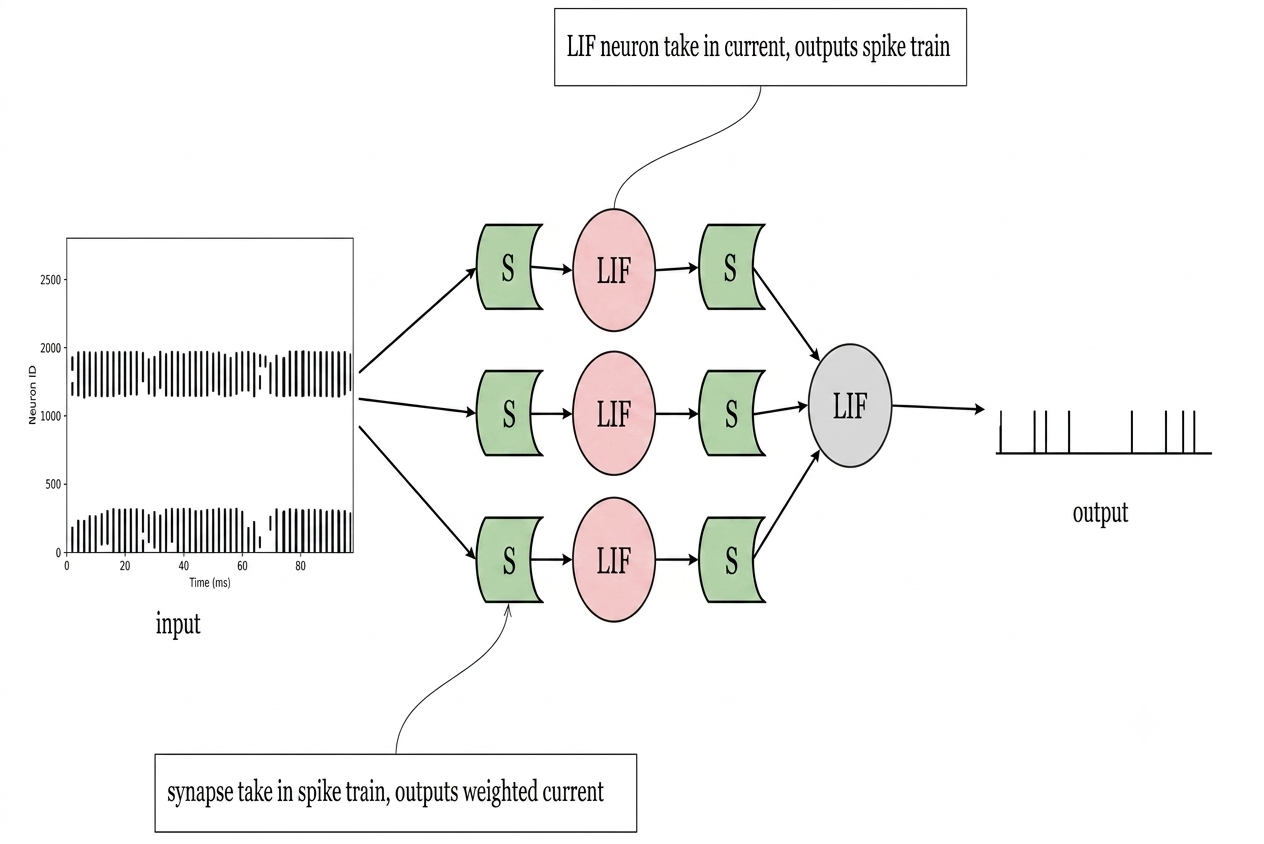
\includegraphics[width=0.85\columnwidth]{assets/images/NN.png}
    \captionof{figure}{Spiking Neural Network data flow: parallel spike-train inputs are weighted by synapse blocks (S), integrated by Leaky Integrate-and-Fire (LIF) neurons, and combined into a sparse output spike train. Diagram prepared by the author, illustrating the LIF formulation described by Maass [2] and Roy et al. [4].}
\end{minipage}
  \end{center}
\vspace{-0.35em}

  \subsubsection*{Neuromorphic Computing Architecture}
  Neuromorphic computing architecture is a brain-inspired system design that replicates the structure, functionality, and communication methods of biological neural networks. Unlike conventional computing systems that rely on a strict separation between memory and processing units, neuromorphic architecture integrates both functions into a unified framework, allowing computation to occur in a more natural, efficient, and parallel manner.
  \begin{enumerate}\justifying
    \item \textbf{Core Design Principle}
      \begin{itemize}
        \item \textbf{Eliminates bottlenecks:} traditional systems separate the CPU and memory, causing data-movement delays.
        \item Integrated units: combines processing (neurons) and memory (synapses) into a single framework.
        \item \textbf{High efficiency:} reduces data movement, improving speed and lowering power use — the same principle exploited by IBM NorthPole [12].
      \end{itemize}
    \item \textbf{Event-Driven Processing}
      \begin{itemize}
        \item \textbf{Spike-activated:} systems process data only when triggered by meaningful events (spikes).
        \item \textbf{Idle by default:} chips remain largely inactive until input signals cross a specific threshold.
        \item \textbf{Key benefit:} saves energy and enables real-time responsiveness, though only for sparse, temporally structured inputs.
      \end{itemize}

    \item \textbf{Parallel Structure}
      \begin{itemize}
        \item \textbf{Massively concurrent:} large numbers of artificial neurons compute simultaneously instead of sequentially.
        \item \textbf{Decentralised control:} processing is distributed locally across multiple independent cores.
        \item \textbf{Key benefit:} low latency and efficient scaling for workloads that are naturally distributable.
      \end{itemize}
    \item \textbf{Key Components}
      \begin{enumerate}[label=(\alph*)]
        \item \textbf{Artificial Neurons} — receive input spikes, integrate information over time, and fire an output spike when a threshold is reached, mimicking biological neuron behaviour.
        \item \textbf{Synaptic Connections} — weighted links between neurons that determine signal strength and also serve as the system's memory, since learned information is stored in synaptic weights.
        \item \textbf{Communication Networks} — neuromorphic systems use asynchronous, spike-based communication such as Address Event Representation (AER) and event-driven routing, so that only active neurons communicate.
        \item \textbf{Learning Circuits (Plasticity Mechanisms)} — adapt synaptic strengths over time using rules such as Spike-Timing-Dependent Plasticity (STDP) and Hebbian learning, enabling on-chip learning without an external training system.
      \end{enumerate}
  \end{enumerate}

  \begin{center}
\vspace{-0.5em}
\begin{minipage}{0.98\columnwidth}
\centering
    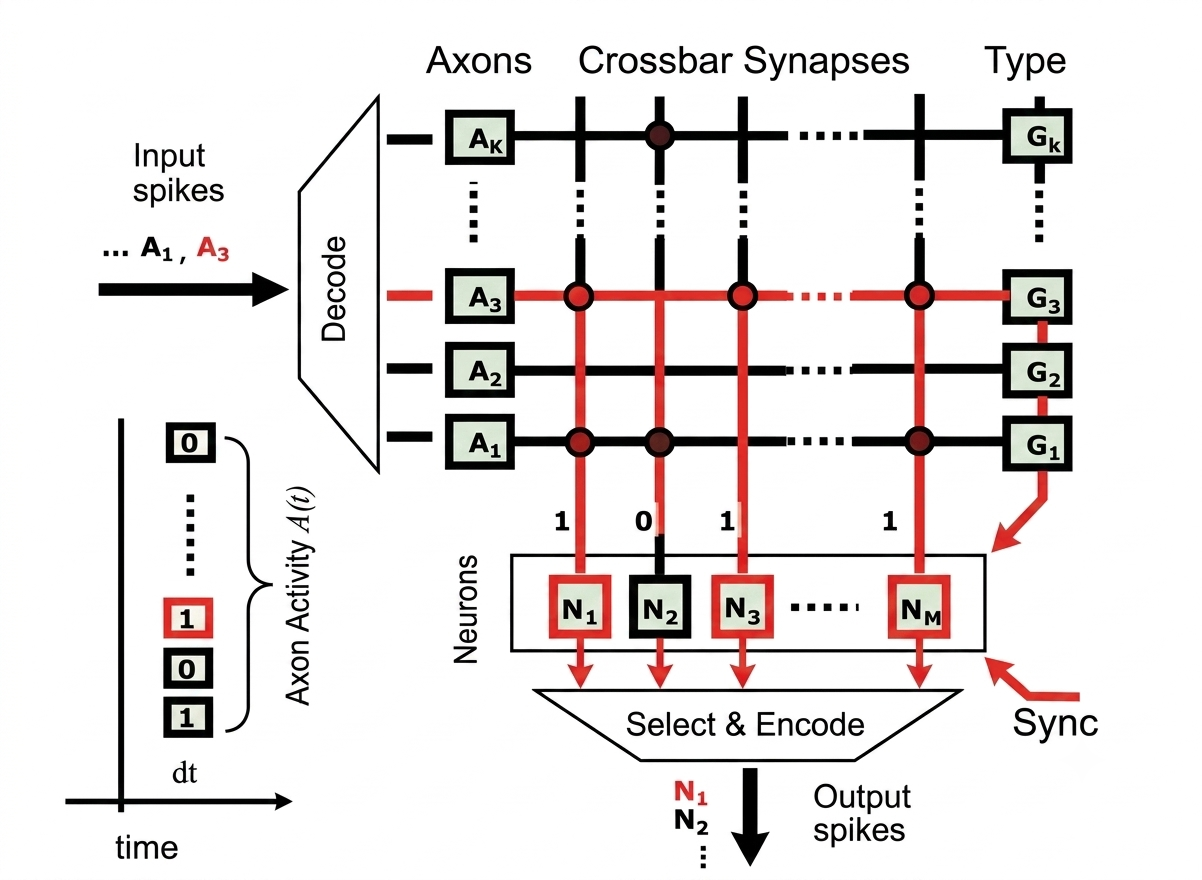
\includegraphics[width=0.72\columnwidth]{assets/images/NMC.png}
    \captionof{figure}{Simplified neuromorphic crossbar architecture: input spikes are decoded onto axons, weighted at crossbar synapse junctions, integrated by neurons $N_1$--$N_n$, and re-encoded into output spikes. Diagram prepared by the author, conceptually based on the crossbar-array designs surveyed by Schuman et al. [9].}
\end{minipage}
  \end{center}
\vspace{-0.35em}

  \subsubsection*{Major Neuromorphic Chips — Established Systems}
  \begin{enumerate}
    \item \textbf{Intel Loihi:} Intel's first-generation Loihi chip (2018) implements 131,072 neurons and 130 million synapses on a 14 nm process, using asynchronous spiking neural networks with on-chip STDP-based learning [6]. Loihi has been used mainly in robotics and academic research rather than commercial products.
    \item \textbf{IBM TrueNorth:} IBM's TrueNorth (2014) was one of the earliest large-scale neuromorphic processors, implementing 1 million neurons and 256 million synapses on a 28 nm process at roughly 65 mW per chip [5]. TrueNorth demonstrated the feasibility of implementing million-neuron systems in hardware, though, like Loihi, it saw limited commercial uptake.
    \item \textbf{SpiNNaker:} The SpiNNaker project, developed at the University of Manchester, uses massively parallel ARM-core clusters for real-time neural simulation. It is primarily used for large-scale simulation of biological brain models rather than deployed AI inference [8].
    \item \textbf{BrainScaleS:} BrainScaleS is a European neuromorphic platform that uses analog (rather than digital) neural computation to achieve very high-speed, accelerated brain simulation, trading digital precision for analog speed and energy efficiency [10].
  \end{enumerate}
  \subsubsection*{Recent Developments (2021–2026)}
  The years since the systems above were introduced have seen two significant developments that move neuromorphic computing closer to practical relevance, alongside continued evidence that broad commercial adoption remains distant.
  \begin{itemize}\justifying
    \item \textbf{Intel Loihi 2 and Hala Point:} Intel's second-generation Loihi 2 (2021) improved processing speed roughly tenfold over the original Loihi while supporting more flexible neuron models. In 2024 Intel assembled 1,152 Loihi 2 chips into Hala Point, a research-scale system with 1.15 billion neurons and 128 billion synapses, sustaining approximately 20 petaops at over 15 trillion 8-bit operations per second per watt — the largest neuromorphic system built to date [11].
    \item \textbf{IBM NorthPole:} IBM's NorthPole (2023), described by Modha et al. in Science, is not a spiking chip but a brain-inspired inference accelerator that eliminates off-chip memory access by co-locating compute and memory across its cores. On the ResNet-50 image-classification benchmark, NorthPole reports roughly 25× higher energy efficiency (frames per second per watt) and 5× higher space efficiency than a comparable 12 nm-class GPU [12]. Because NorthPole targets inference only and does not use spikes, its inclusion illustrates that “brain-inspired” efficiency gains can be achieved through memory-compute co-location alone, independent of spiking dynamics.
    \item \textbf{Edge-Oriented Commercial Chips:} Alongside these large research systems, edge-focused neuromorphic chips such as BrainChip's Akida and Innatera's mixed-signal T1 have reached commercial, milliwatt-class deployment in cameras, sensors, and wearables — a narrower but more immediately commercial application than the large research systems above.
  \end{itemize}

  \subsubsection*{Quantitative Comparison of Neuromorphic Systems}
  The table below consolidates the quantitative specifications discussed above to allow direct comparison across generations and design philosophies.
\end{multicols}
\begin{table}[tb]
\centering
\caption{Quantitative comparison of representative neuromorphic and brain-inspired computing systems.}
\small
  \setlength{\tabcolsep}{3pt}
  \renewcommand{\arraystretch}{1.2}
  \begin{tabular}{@{}>{\RaggedRight\arraybackslash}p{0.18\textwidth}
      >{\RaggedRight\arraybackslash}p{0.11\textwidth}
      >{\RaggedRight\arraybackslash}p{0.12\textwidth}
      >{\RaggedRight\arraybackslash}p{0.10\textwidth}
      >{\RaggedRight\arraybackslash}p{0.20\textwidth}
    >{\RaggedRight\arraybackslash}p{0.21\textwidth}@{}}
    \toprule
    \textbf{Chip / System} & \textbf{Neurons} & \textbf{Synapses} & \textbf{Process Node} & \textbf{Power / Efficiency} & \textbf{Status / Notes} \\
    \midrule
    IBM TrueNorth (2014) & 1 million & 256 million & 28 nm & $\sim$65 mW/chip & Early large-scale proof of concept [5] \\
    Intel Loihi (2018) & 131,072 & 130 million & 14 nm & Sub-100 mW typical & Research/robotics use [6] \\
    Intel Loihi 2 (2021) & Up to 1 million/chip & 120 million/chip & Intel 4 (7 nm-class) & $\sim$10$\times$ faster than Loihi 1 & Basis for Hala Point [11] \\
    Intel Hala Point (2024) & 1.15 billion (system) & 128 billion (system) & Intel 4 & 20 petaops; $>$15 TOPS/W & 1,152 Loihi 2 chips; research-scale [11] \\
    IBM NorthPole (2023) & 224M-parameter-class arrays & N/A (dense on-chip weights) & 12 nm & 25$\times$ FPS/W vs. comparable 12 nm GPU on ResNet-50 & Not spike-based; inference-only ASIC [12] \\
    \bottomrule
  \end{tabular}
\end{table}
\vspace{-0.18em}

\begin{multicols}{2}
  Table~2 (above) quantifies representative neuromorphic and brain-inspired systems.

  \subsubsection*{Working Principle of Neuromorphic Chips}
  Neuromorphic chips process information through interconnected artificial neurons. When a neuron receives sufficient input signals, it generates a spike that propagates to connected neurons. The operation can be summarised as follows: (1) sensory data is received as electrical signals; (2) artificial neurons integrate the signals; (3) spikes are transmitted across synapses; (4) synaptic weights are updated during learning; (5) output decisions are generated. This process closely resembles biological neural communication, though the precision with which it is implemented varies considerably across the chips discussed in Sections 3.5–3.6.

  \subsubsection*{Advantages of Neuromorphic Computing}
  \begin{enumerate}
    \item \textbf{Energy Efficiency:} Neuromorphic systems can consume significantly less power than traditional processors on workloads that suit event-driven computation, making them attractive for battery-powered devices and edge computing.
    \item \textbf{Real-Time Processing:} Parallel, event-driven architecture allows rapid processing for real-time decision-making in autonomous systems and robotics.
    \item \textbf{Scalability:} Architectures such as Loihi 2 and Hala Point demonstrate that neuromorphic systems can scale to billions of neurons and synapses, at least at the research-system level [11].
    \item \textbf{Adaptive Learning:} On-chip plasticity mechanisms such as STDP allow neuromorphic chips to adapt dynamically to environmental changes without complete retraining.
    \item \textbf{Fault Tolerance:} The distributed nature of neural systems allows neuromorphic chips to continue functioning even if some components fail.
  \end{enumerate}

  \subsubsection*{Applications of Neuromorphic Computing}
  \begin{enumerate}\justifying
    \item \textbf{Robotics:} Neuromorphic chips enable robots to process sensory information and react quickly to changing environments, supporting navigation and object recognition.
    \item \textbf{Autonomous Vehicles:} Self-driving cars require rapid decision-making based on sensor data; neuromorphic processors can improve efficiency in object detection, collision avoidance, and navigation.
    \item \textbf{Healthcare:} Applications include brain–machine interfaces, prosthetic devices, medical diagnosis, and neural monitoring systems.
    \item \textbf{Edge Computing:} Edge devices such as smartphones, IoT sensors, and drones benefit from low-power neuromorphic processing, and are, in practice, the segment where commercial deployment (Akida, Innatera T1) is furthest along.
    \item \textbf{Cybersecurity:} Neuromorphic systems can detect abnormal patterns and cyber threats in real time using adaptive learning mechanisms.
    \item \textbf{Speech and Image Recognition:} Neuromorphic processors can recognise speech patterns, facial expressions, and visual objects with reduced energy consumption relative to GPU-based pipelines, on the specific benchmark tasks reported in the literature.
  \end{enumerate}

  \subsubsection*{Critical Analysis and Challenges}
  While Sections 3.5–3.10 describe genuine engineering achievements, a critical reading of the neuromorphic computing literature reveals that the field has been described as “five years away” from commercial relevance for approximately fifteen years, and several structural issues explain why.
  \begin{enumerate}\justifying
    \item \textbf{Workload Mismatch:} The energy-efficiency figures reported for Hala Point and NorthPole are workload-specific rather than general-purpose. Sparse, temporally structured, event-driven tasks — continuous auditory processing, certain optimisation problems, and some robotics control loops — map naturally onto neuromorphic hardware. Standard image classification pipelines, and especially transformer-based large language models that dominate contemporary AI workloads, rely on dense matrix multiplication and do not map efficiently onto spike-based substrates. This means the headline efficiency multipliers cannot be generalised to “AI workloads” as a whole.
    \item \textbf{Software and Programming Ecosystem Gap:} Unlike GPU computing, which matured around a single dominant programming model (CUDA), the neuromorphic field remains fragmented across at least five materially different architectures — Loihi 2, SpiNNaker2, Akida, NorthPole, and Innatera T1 — each with its own programming model and toolchain. This fragmentation, more than any hardware limitation, is the primary obstacle to porting existing AI workloads onto neuromorphic substrates.
    \item \textbf{Hardware Complexity and Programming Difficulty:} Designing chips that accurately mimic biological neural systems remains highly complex, and neuromorphic programming models differ substantially from conventional software engineering practice, raising the barrier to entry for developers.
    \item \textbf{Limited Commercial Adoption:} With the partial exception of edge-oriented chips such as Akida and Innatera T1, neither Intel nor IBM has shipped a production, general-purpose commercial neuromorphic product; current large-scale deployments remain research partnerships and government-funded systems rather than mainstream commercial infrastructure.
    \item \textbf{Lack of Standardization:} There are no universal standards for neuromorphic hardware or software design, which complicates benchmarking, cross-vendor comparison, and the kind of ecosystem effects that accelerated GPU adoption.
    \item \textbf{Scalability Challenges:} Although Hala Point demonstrates scalability to billions of neurons, this required assembling over a thousand individual chips; whether such multi-chip systems can be made cost-effective and power-efficient at data-centre scale, rather than as research demonstrations, remains an open question.
  \end{enumerate}

  \subsubsection*{Future Scope of Neuromorphic Computing}
  Neuromorphic computing is likely to retain a meaningful, if narrower than initially projected, role in future AI systems — particularly where energy constraints dominate, such as edge AI, wearables, and always-on sensing.
  Future developments that could broaden this role include:
  \begin{itemize}\justifying
    \item A unifying software framework analogous to CUDA, potentially built around open efforts such as Intel's Lava
    \item Advanced autonomous robots exploiting low-latency, event-driven sensing
    \item Energy-efficient AI hardware for edge and wearable deployment
    \item Brain-computer interfaces requiring real-time, low-power neural signal processing
    \item Hybrid architectures that combine neuromorphic front-ends with conventional accelerators for dense computation
  \end{itemize}
  As AI continues to expand into everyday life, neuromorphic systems are likely to remain a specialised complement to, rather than a wholesale replacement for, GPU- and TPU-based computing, at least over the near-to-medium term.

  \subsection*{\centering\uppercase{Conclusion}}
  Neuromorphic computing represents a genuine and well-documented engineering achievement in brain-inspired hardware design, with systems such as Intel's Hala Point and IBM's NorthPole demonstrating substantial, quantifiable efficiency gains on the specific workloads for which they were designed. At the same time, a critical assessment of the field shows that these gains are narrower in scope than early enthusiasm suggested: the mismatch between spike-based hardware and the dense-matrix workloads that dominate modern AI, combined with a fragmented and immature software ecosystem, has kept neuromorphic computing largely confined to research systems and niche edge deployments rather than mainstream commercial adoption.

  \noindent
  Continued progress in hardware scaling, exemplified by Hala Point, and in memory-compute co-location, exemplified by NorthPole, suggests the field is advancing on solid engineering grounds. Whether it achieves broad commercial relevance will likely depend less on further hardware gains and more on the emergence of a standardised programming model and a clearer identification of the workloads for which brain-inspired computation offers a decisive advantage

  \subsection*{\centering\uppercase{References}}

  \begin{enumerate}
    \item C. Mead, “Neuromorphic electronic systems,” Proceedings of the IEEE, vol. 78, no. 10, pp. 1629–1636, 1990.
    \item W. Maass, “Networks of spiking neurons: The third generation of neural network models,” Neural Networks, vol. 10, no. 9, pp. 1659–1671, 1997.
    \item G. Indiveri and S.-C. Liu, “Memory and information processing in neuromorphic systems,” Proceedings of the IEEE, vol. 103, no. 8, pp. 1379–1397, 2015.
    \item K. Roy, A. Jaiswal, and P. Panda, “Towards spike-based machine intelligence with neuromorphic computing,” Nature, vol. 575, pp. 607–617, 2019.
    \item P. A. Merolla et al., “A million spiking-neuron integrated circuit with a scalable communication network and interface,” Science, vol. 345, no. 6197, pp. 668–673, 2014.
    \item M. Davies et al., “Loihi: A neuromorphic manycore processor with on-chip learning,” IEEE Micro, vol. 38, no. 1, pp. 82–99, 2018.
    \item A. R. Young et al., “A review of spiking neuromorphic hardware communication systems,” IEEE Access, vol. 7, pp. 135606–135620, 2019.
    \item S. B. Furber et al., “The SpiNNaker project,” Proceedings of the IEEE, vol. 102, no. 5, pp. 652–665, 2014.
    \item C. D. Schuman et al., “A survey of neuromorphic computing and neural networks in hardware,” arXiv preprint arXiv:1705.06963, 2017.
    \item C. Pehle et al., “The BrainScaleS-2 accelerated neuromorphic system with hybrid plasticity,” arXiv preprint arXiv:2201.11063, 2022.
    \item Intel Corporation, “Intel Builds World’s Largest Neuromorphic System to Enable More Sustainable AI (Hala Point),” Intel Newsroom, Apr. 2024. Loihi 2 architecture details from Intel Neuromorphic Research Community technical documentation.
    \item D. S. Modha et al., “Neural inference at the frontier of energy, space, and time,” Science, vol. 382, no. 6668, pp. 329–335, 2023. DOI: 10.1126/science.adh1174.
    \item Recent review: “A New Era in Computing: A Review of Neuromorphic Computing Chip Architecture and Applications,” Chips, vol. 5, no. 1, article 3, 2026. DOI: 10.3390/chips5010003.
  \end{enumerate}
\end{multicols}
% Full-width info box outside multicols
\begin{center}
  \begin{minipage}{\textwidth}
    \begin{tcolorbox}[
  colback=yellow!7,
  colframe=blue!35!black,
  colbacktitle=yellow!75!orange,
  coltitle=blue!25!black,
  title=\MakeUppercase{Did You Know?},
  fonttitle=\large\bfseries\sffamily,
  toptitle=1.5mm,
  bottomtitle=1.5mm,
  boxrule=0.7pt,
  arc=0mm,
  left=4mm,
  right=4mm,
  top=2.5mm,
  bottom=2.5mm
]
\footnotesize
\noindent
\begin{minipage}[t]{0.48\linewidth}
  {\sffamily\bfseries\textcolor{blue!35!black}{THE 2.15 dB DIFFERENCE}}\par
  A half-wave dipole has approximately \(2.15\text{ dBi}\) gain. Therefore,
  \(0\text{ dBd}=2.15\text{ dBi}\).

  \vspace{0.18em}
  {\sffamily\bfseries\textcolor{blue!35!black}{GAIN REDIRECTS ENERGY}}\par
  Antenna gain does not create extra transmitter power; it concentrates the
  available radiation more strongly in selected directions.
\end{minipage}
\hfill
\begin{minipage}[t]{0.48\linewidth}
  {\sffamily\bfseries\textcolor{blue!35!black}{THE 3 dB RULE}}\par
  A \(3\text{ dB}\) increase represents approximately twice the power, while
  a \(3\text{ dB}\) decrease represents half the power.

  \vspace{0.18em}
  {\sffamily\bfseries\textcolor{blue!35!black}{FREQUENCY SETS THE SCALE}}\par
  Since \(\lambda=c/f\), antennas designed for higher frequencies are
  generally physically smaller than antennas designed for lower frequencies.
\end{minipage}
\end{tcolorbox}
  \end{minipage}
\end{center}

\begin{center}
  \section{\capitalisewords{Role of ISRO in Technological Advancement}}
  Suprio Dutta, 3$^{rd}$ Year, ECE
\end{center}

\setcounter{figure}{0}

\begingroup
\makeatletter
\renewcommand\subsection{\@startsection{subsection}{2}{\z@}%
  {1.2ex}{0.6ex}{\normalfont\large\bfseries}}
\makeatother
\begin{multicols}{2}
  \begin{abstract}
    \bfseries
    ISRO viz Indian Space Research Organisation established in 1969 was never solely about rockets[1]. From the
    beginning it mainly focused on solving practical problems such as delivering weather data to coastal fishermen,
    emergency communication after disaster and providing healthcare and education to remote and inaccessible
    villages. This thinking carried into the missions as well. Chandrayaan-1[2] confirmed water molecules on the
    lunar surface, reshaping international lunar science. Mangalyaan reached Mars orbit on its first attempt and did
    so at a cost almost half of the Interstellar movie. This is because, India had access to limited resource and financial
    support as a result engineers had to figure how to stretch out every rupee. Aditya-L1[3], now stationed at the L1
    Lagrange point[4], gives India a route to heliophysics[5], a domain only few agencies currently have access to.
    Most Indian don’t realise we have our own GPS which is NavIC[6] which became one of our greatest asset during
    Operation Sindoor. ISRO satellites are keeping education and telemedicine running in areas where roads and
    electricity are still unreliable. ISRO isn’t operating alone anymore. Private players like Skyroot[7] and Agnikul[8],
    alongside academic partnerships, are developing so rapidly that it’s difficult for a single government agency to
    manage alone. Gaganyaan[9] India's first crewed mission is the most important upcoming project. If it succeeds
    India will be the fourth country to send human to space.
  \end{abstract}

  \subsection*{\centering\uppercase{INTRODUCTION}}
  Space technology plays an important role in day-to-day life. Services such as communication,
  navigation, weather forecasting, disaster warnings and every small services relies heavily on satellites.
  For India, this infrastructure wasn’t borrowed from anyone. Much of it is developed from indigenous
  efforts and homegrown technology.
  ISRO was established in 1969 under Dr. Vikram Sarabhai[10], a scientist who believed, that space
  technology should serve people. That mindset to serve is relevant even today. In its early years, ISRO
  operated on tight budgets and limited access to foreign technology, Despite the scarcity and threat of
  foreign sanction ISRO continued to build its own satellites and launch vehicles rather than depend on
  others. This costed much more time but gave self-reliance in comparison to other agencies.

  \begin{center}
\vspace{-0.5em}
\begin{minipage}{0.98\columnwidth}
\centering
    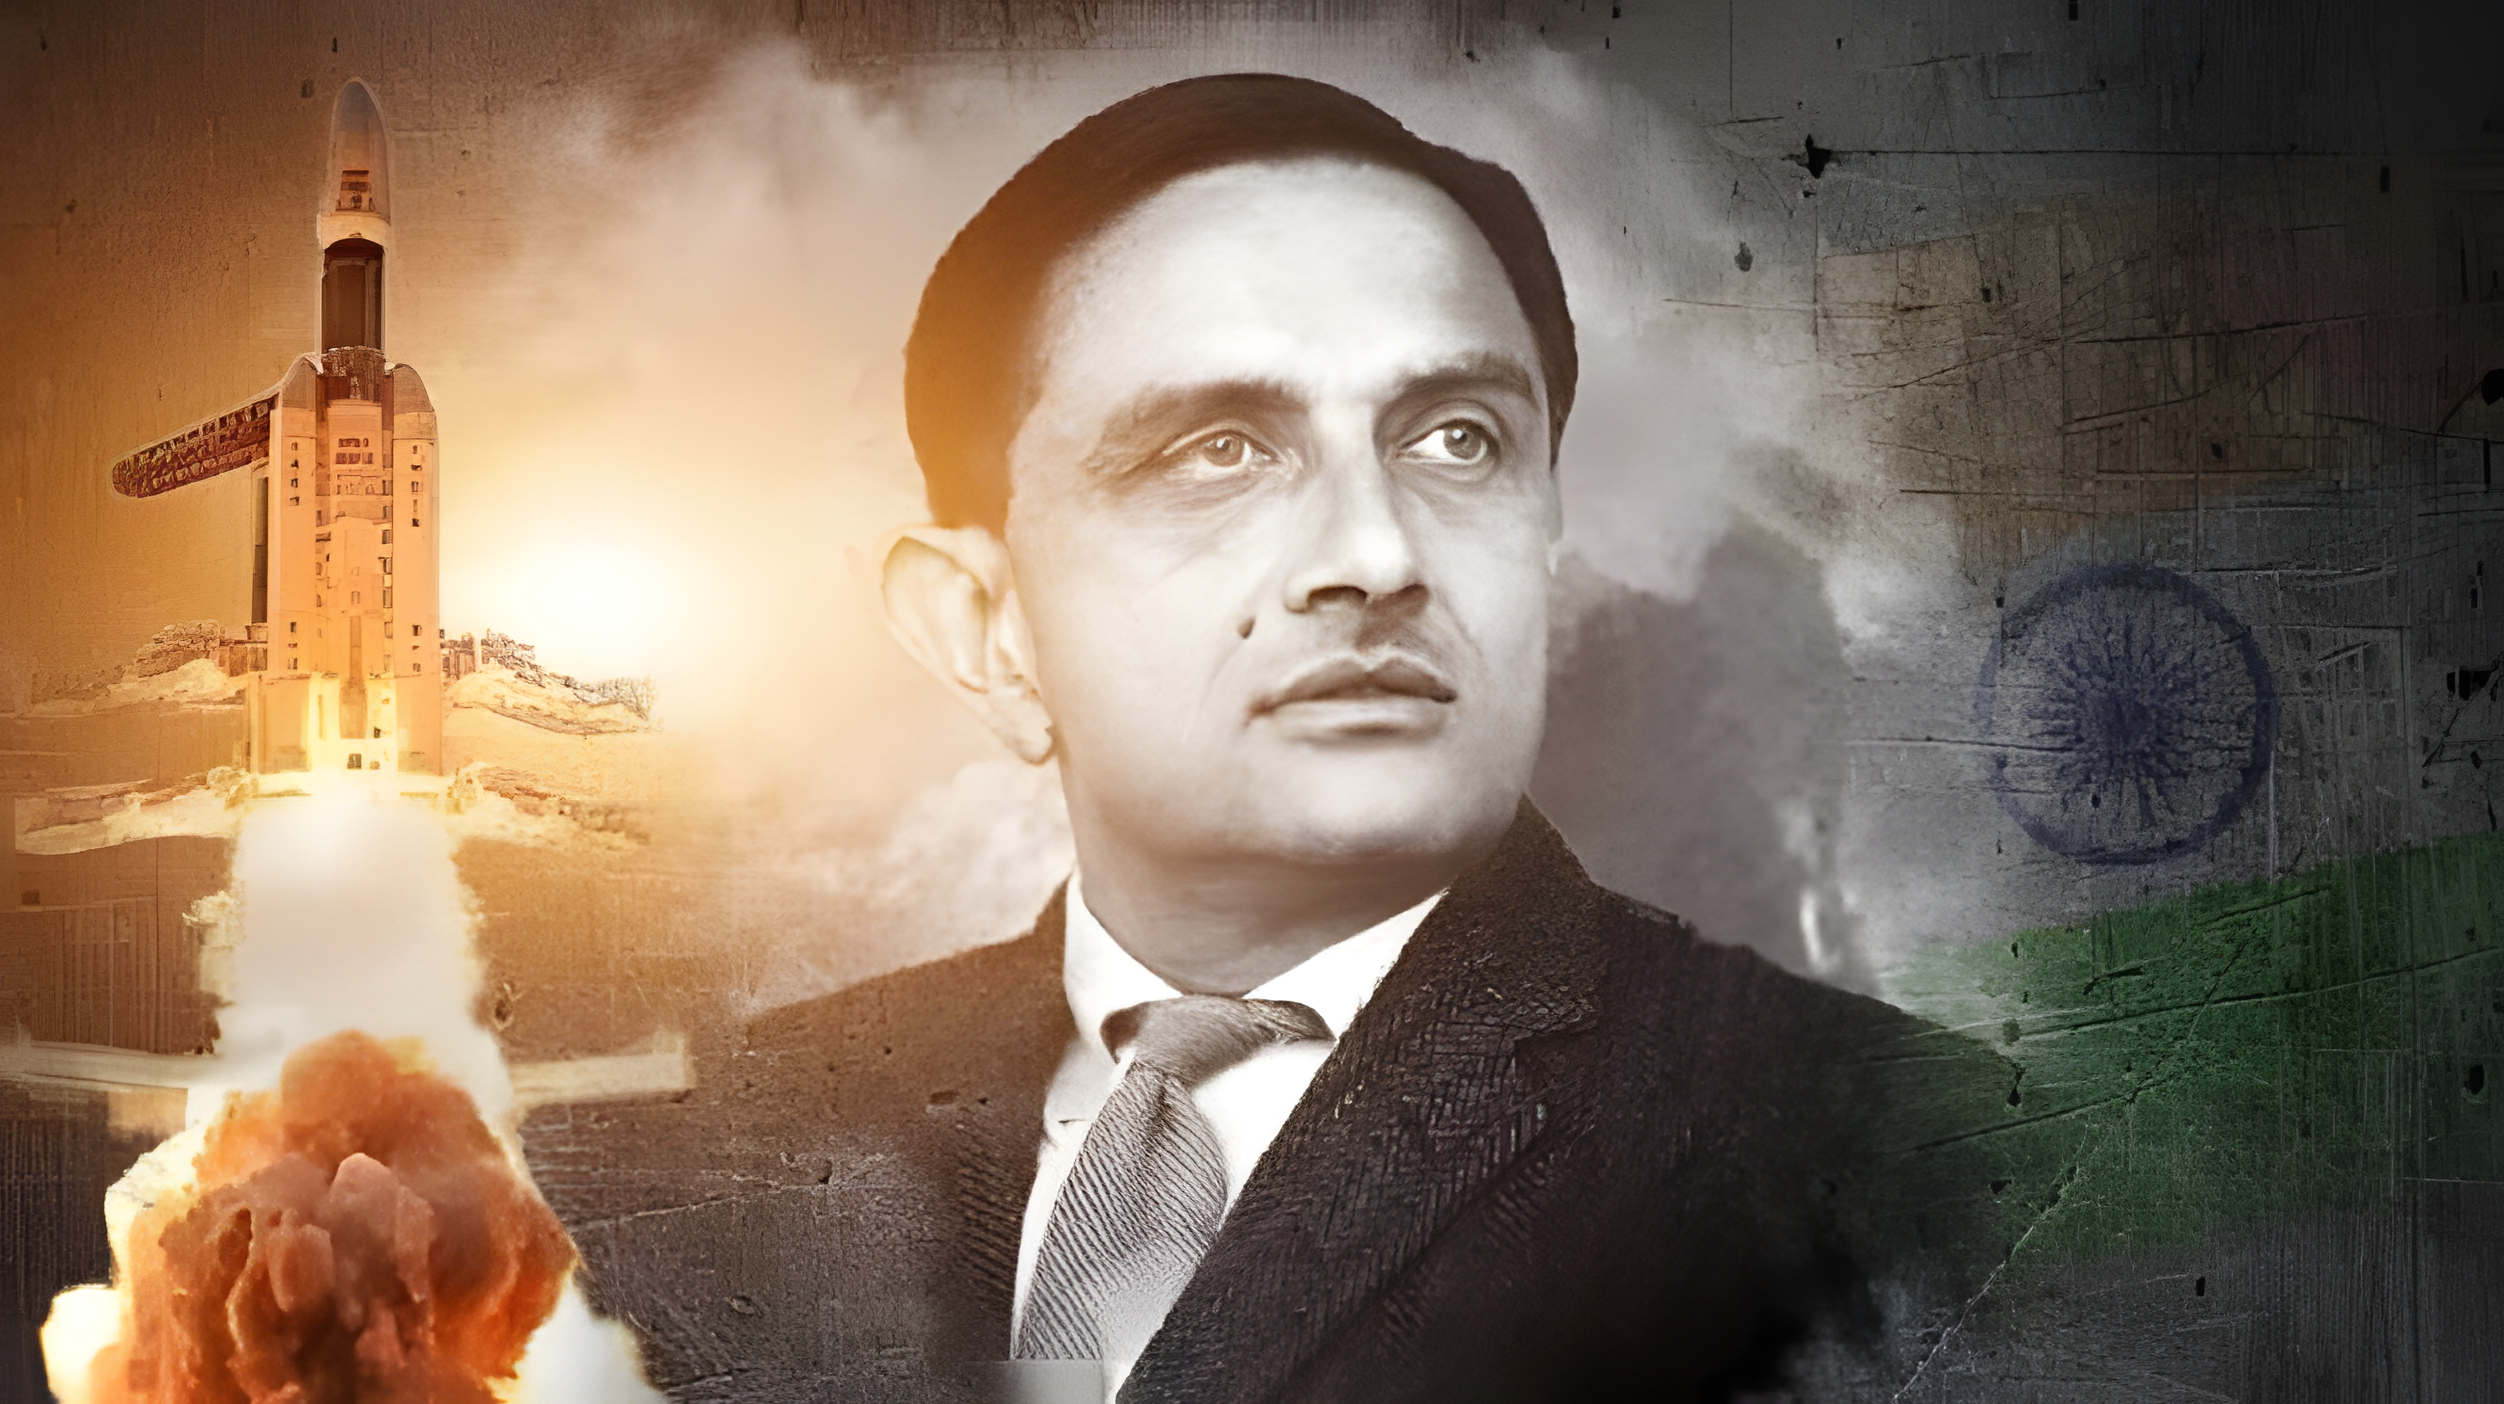
\includegraphics[width=0.85\columnwidth]{assets/images/VAS.png}
    \captionof{figure}{Dr. Vikram Ambalal Sarabhai (12 August 1919 – 30 December 1971) an extraordinary Indian physicist,
      astronomer, and industrialist. He is widely revered as the "Father of the Indian Space Program." He was the
    visionary founder of the Indian Space Research Organisation (ISRO)}
\end{minipage}
  \end{center}

  ISRO does far more than exploration. The satellites carry television signals, mobile networks, monitor
  monsoon pattern, issue warnings during natural calamities., The data are fed into agricultural planning
  and forest management systems across the country. Remote sensing has heavily transformed India’s
  management in water, land, and urban growth. The flagship missions Chandrayaan, Mangalyaan,
  Aditya-L1 grabbed spot in global headlines. NavIC quietly became one of the strategic asset providing
  intel and data to Indian military. Gaganyaan, the upcoming project promises to place India among the very few nations capable of crewed spaceflight. We as Indian students grown up watching ISRO
  succeed, and many are now building the future in AI, robotics, aerospace and more with ISRO.

  {\centering
  \vspace{-0.3em}
  \begin{minipage}{0.98\columnwidth}
  \centering
    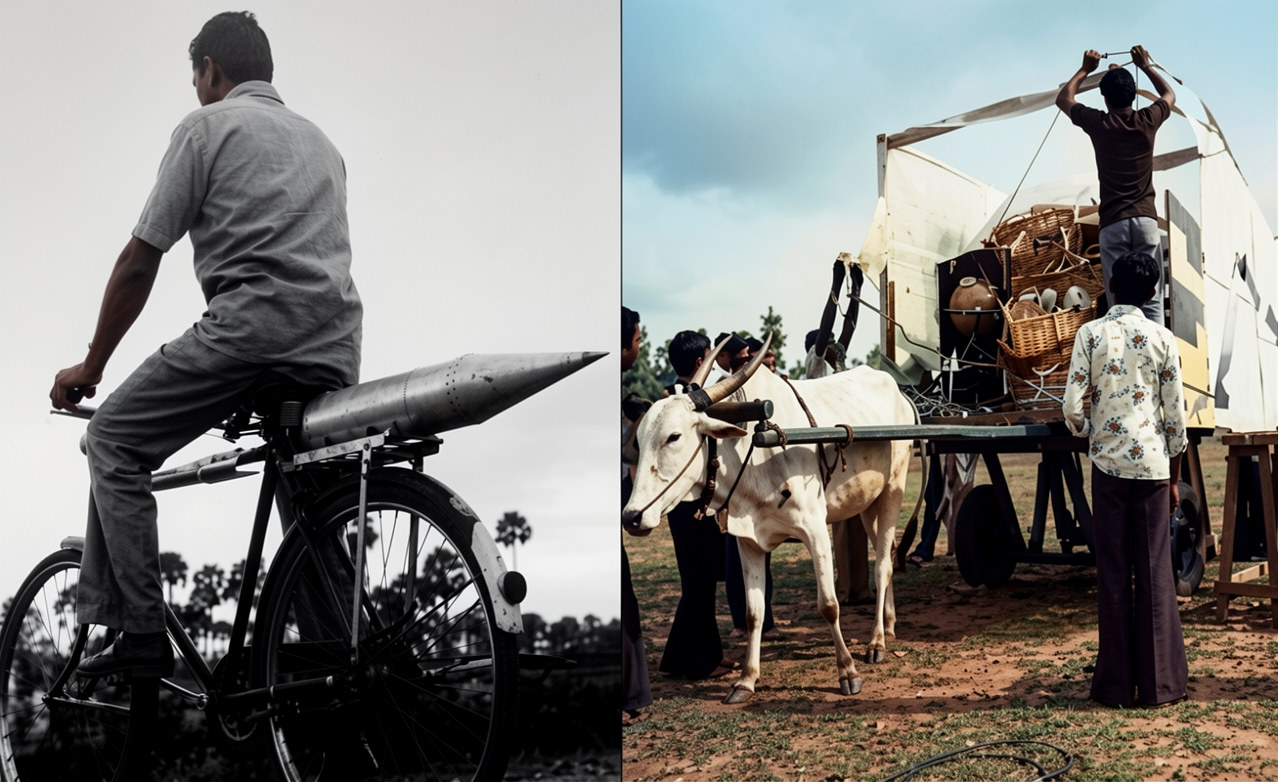
\includegraphics[width=0.85\columnwidth]{assets/images/CRS.jpg}
    \captionof{figure}{The iconic historical photograph shows an Indian space scientist carrying a rocket nose cone on the back of a
      bicycle features scientist CR Satya[11], while a young Dr APJ Abdul Kalam[12] was an integral part of the same
    early rocket launch team.}
  \end{minipage}\par}
  \vspace{-0.4em}

  \subsection*{\centering\uppercase{EVOLUTION AND GROWTH OF ISRO}}
  ISRO began operations on 15 August 1969 i.e. on the eve of India's 22nd Independence Day. Dr.
  Vikram Sarabhai's (one of the founding members) had a straightforward vision i.e. space technology
  should contribute to national development. India recognised early that space research could directly
  address the country's social and economic problems. To solve this the organisation contributed
  tirelessly on research, innovation, and building capability from within despite having limited funding
  or resources during initial years.
  \par\noindent
  The first significant milestone was achieved in 1975 with launch of Aryabhata[13], India's first
  satellite. It wasn't sophisticated according to global standards, but it laid the foundation that could be
  built upon. From there, ISRO developed successive launch vehicle families: the SLV, then the
  PSLV[14], then the GSLV[15], each generation more advanced than the last.

  \begin{center}
\vspace{-0.5em}
\begin{minipage}{0.98\columnwidth}
\centering
    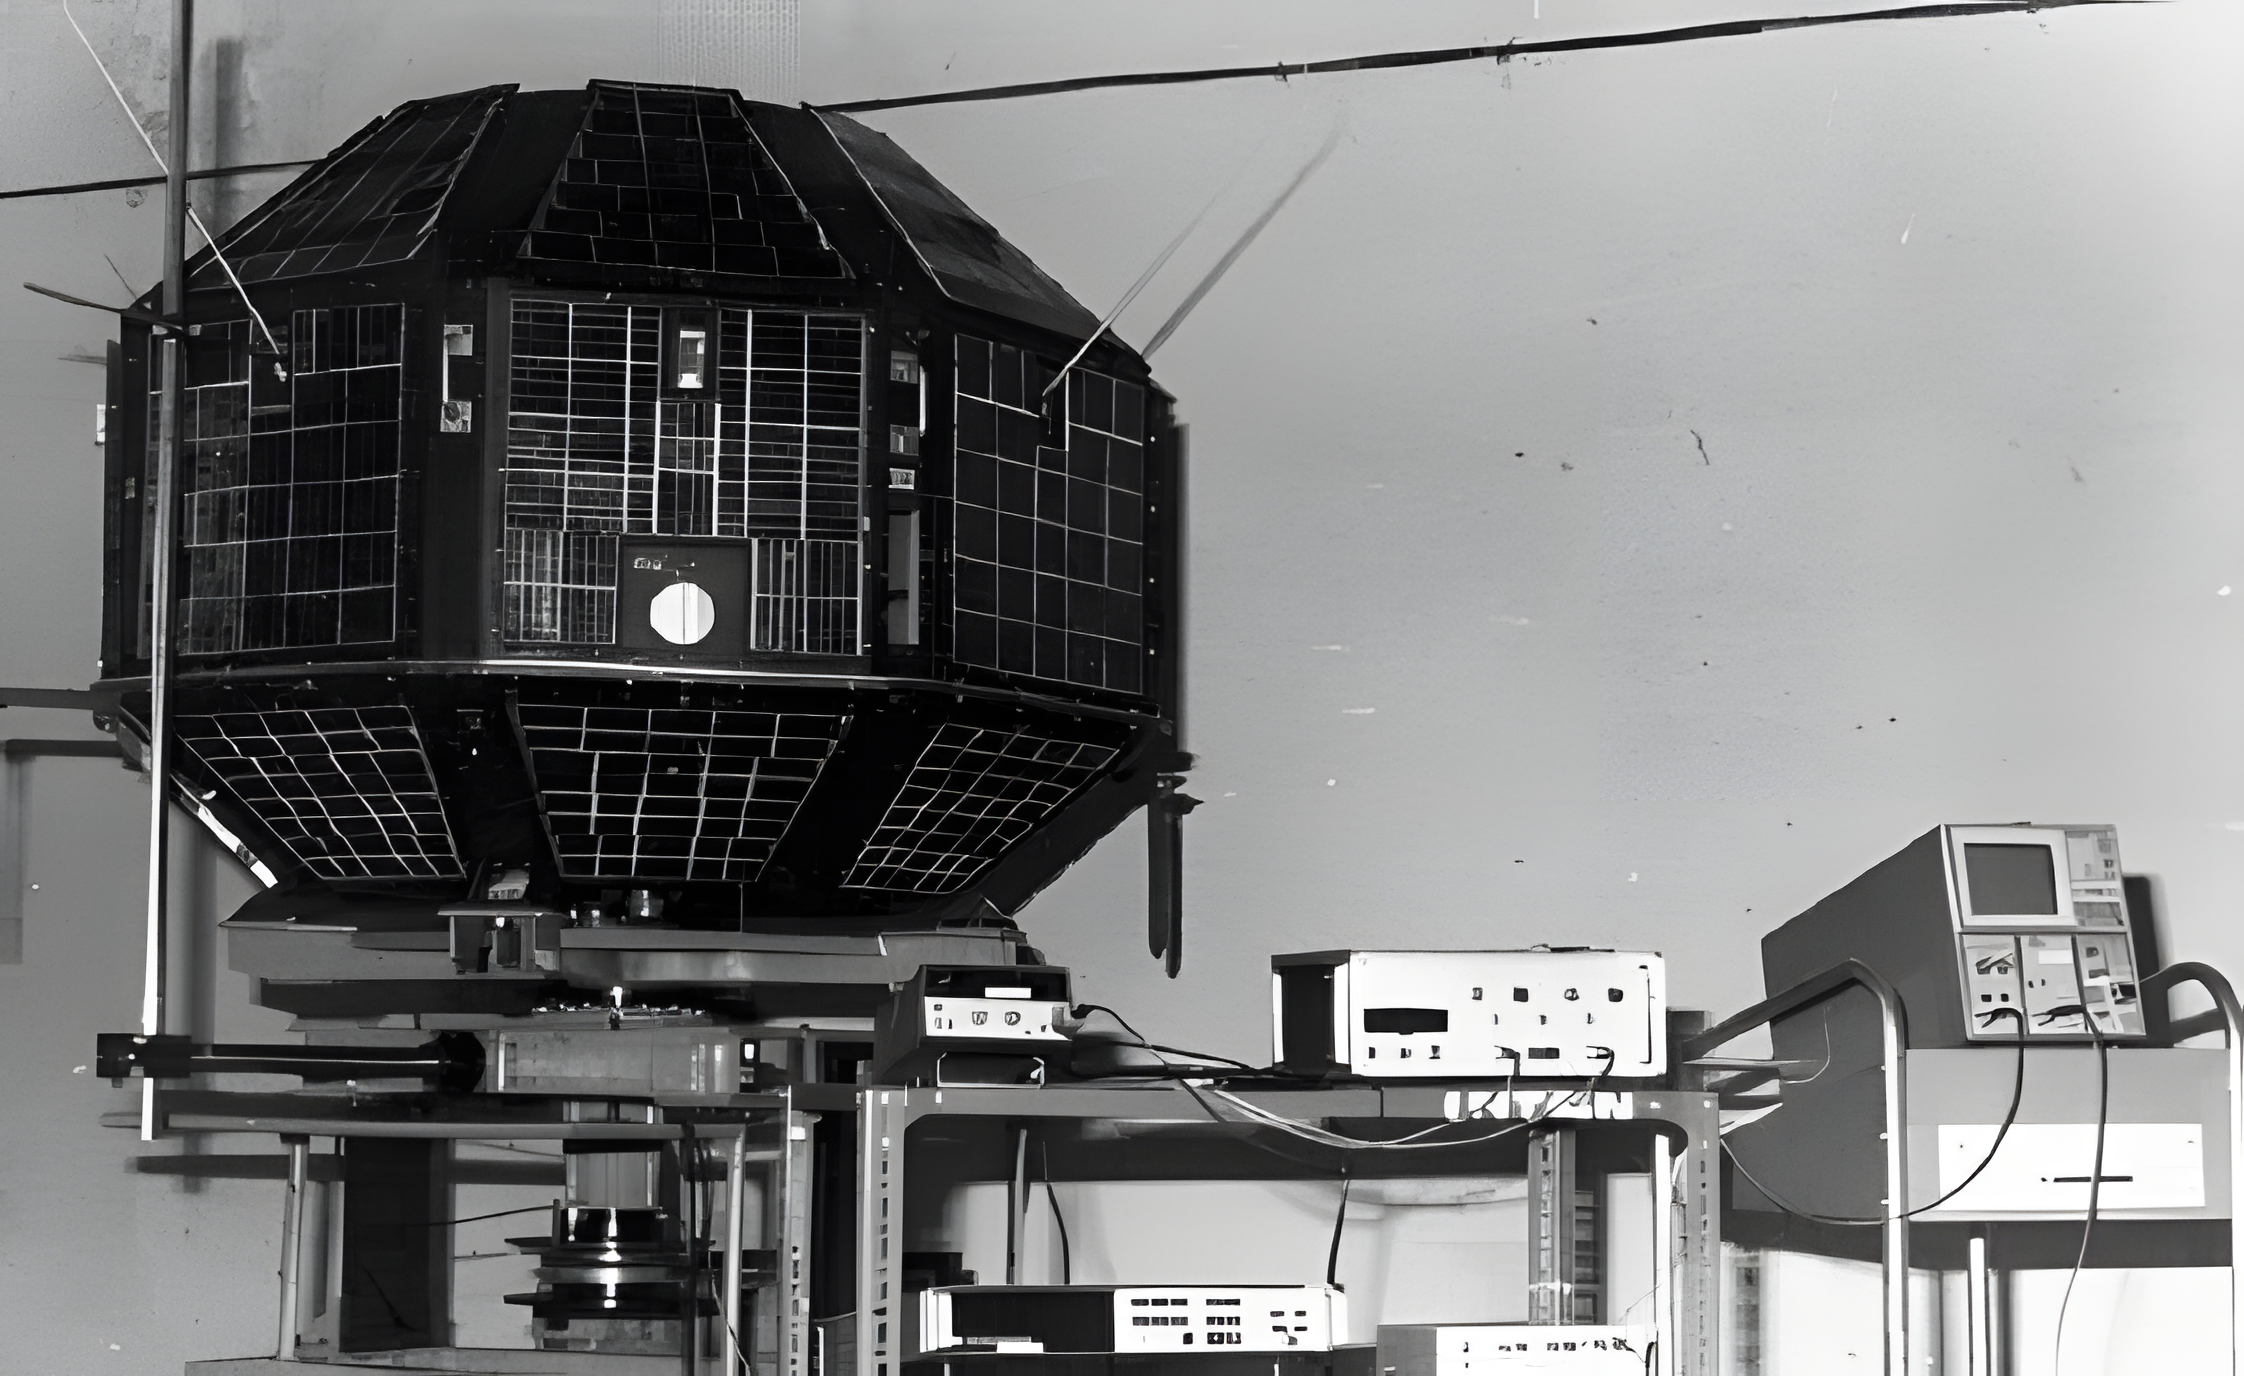
\includegraphics[width=0.7\columnwidth]{assets/images/Aryabhatta.png}
    \captionof{figure}{Aryabhata was India's first satellite, launched on April 19, 1975, from the Kapustin Yar rocket launch site in the Astrakhan
      Oblast, Soviet Union (present-day Russia), utilizing a Kosmos-3M launch vehicle. The 360-kilogram satellite was designed and
    fabricated entirely by the Indian Space Research Organisation (ISRO)}
\end{minipage}
  \end{center}

  The ability to launch independently meant India no longer needed to negotiate with foreign agencies
  every time when it needed to launch a satellite. Out of all in SLV series the PSLV became the standout
  due to its reliable, accurate, and cost-effective approach. As a result it earned international recognition
  and attracted commercial launches from foreign clients such as SpaceX, NASA. This proves the
  reliability and success of this organisation. ISRO's trajectory is worth noting: technological
  advancement doesn't require unlimited budgets or inherited infrastructure. All it takes is clear
  priorities, patience, and scientists willing to solve real life problems without shortcuts. India built all
  three from itself and now the results speak for themselves.

  \subsection*{\centering\uppercase{SATELLITE COMMUNICATION AND REMOTE SENSING}}
  One of ISRO's most significant contribution to society is satellite communication. The communication
  satellite carries broadcast signals from radio’s and televisions, telephone services, and internet
  connectivity across the country where uniform infrastructure is impossible due to uneven geography.
  Today Rural districts are now increasingly connected with satellite signals rather than roads and
  railways.
  \par\noindent
  Remote sensing is the most important work, which is rarely talked about. It plays a important role in
  monitoring crop health, track forest cover, measure water reservoir levels. The data are then mapped
  into decisions which affects millions of Indians. Farmers use the data received from satellite on
  weather patterns soil conditions to maintain proper crop yield. Fishermen off India's coastline get real
  time guidance on safe fishing zones, natural calamities like cyclone which is genuinely a life-saving
  information

  \begin{center}
\vspace{-1em}
\begin{minipage}{0.98\columnwidth}
\centering
    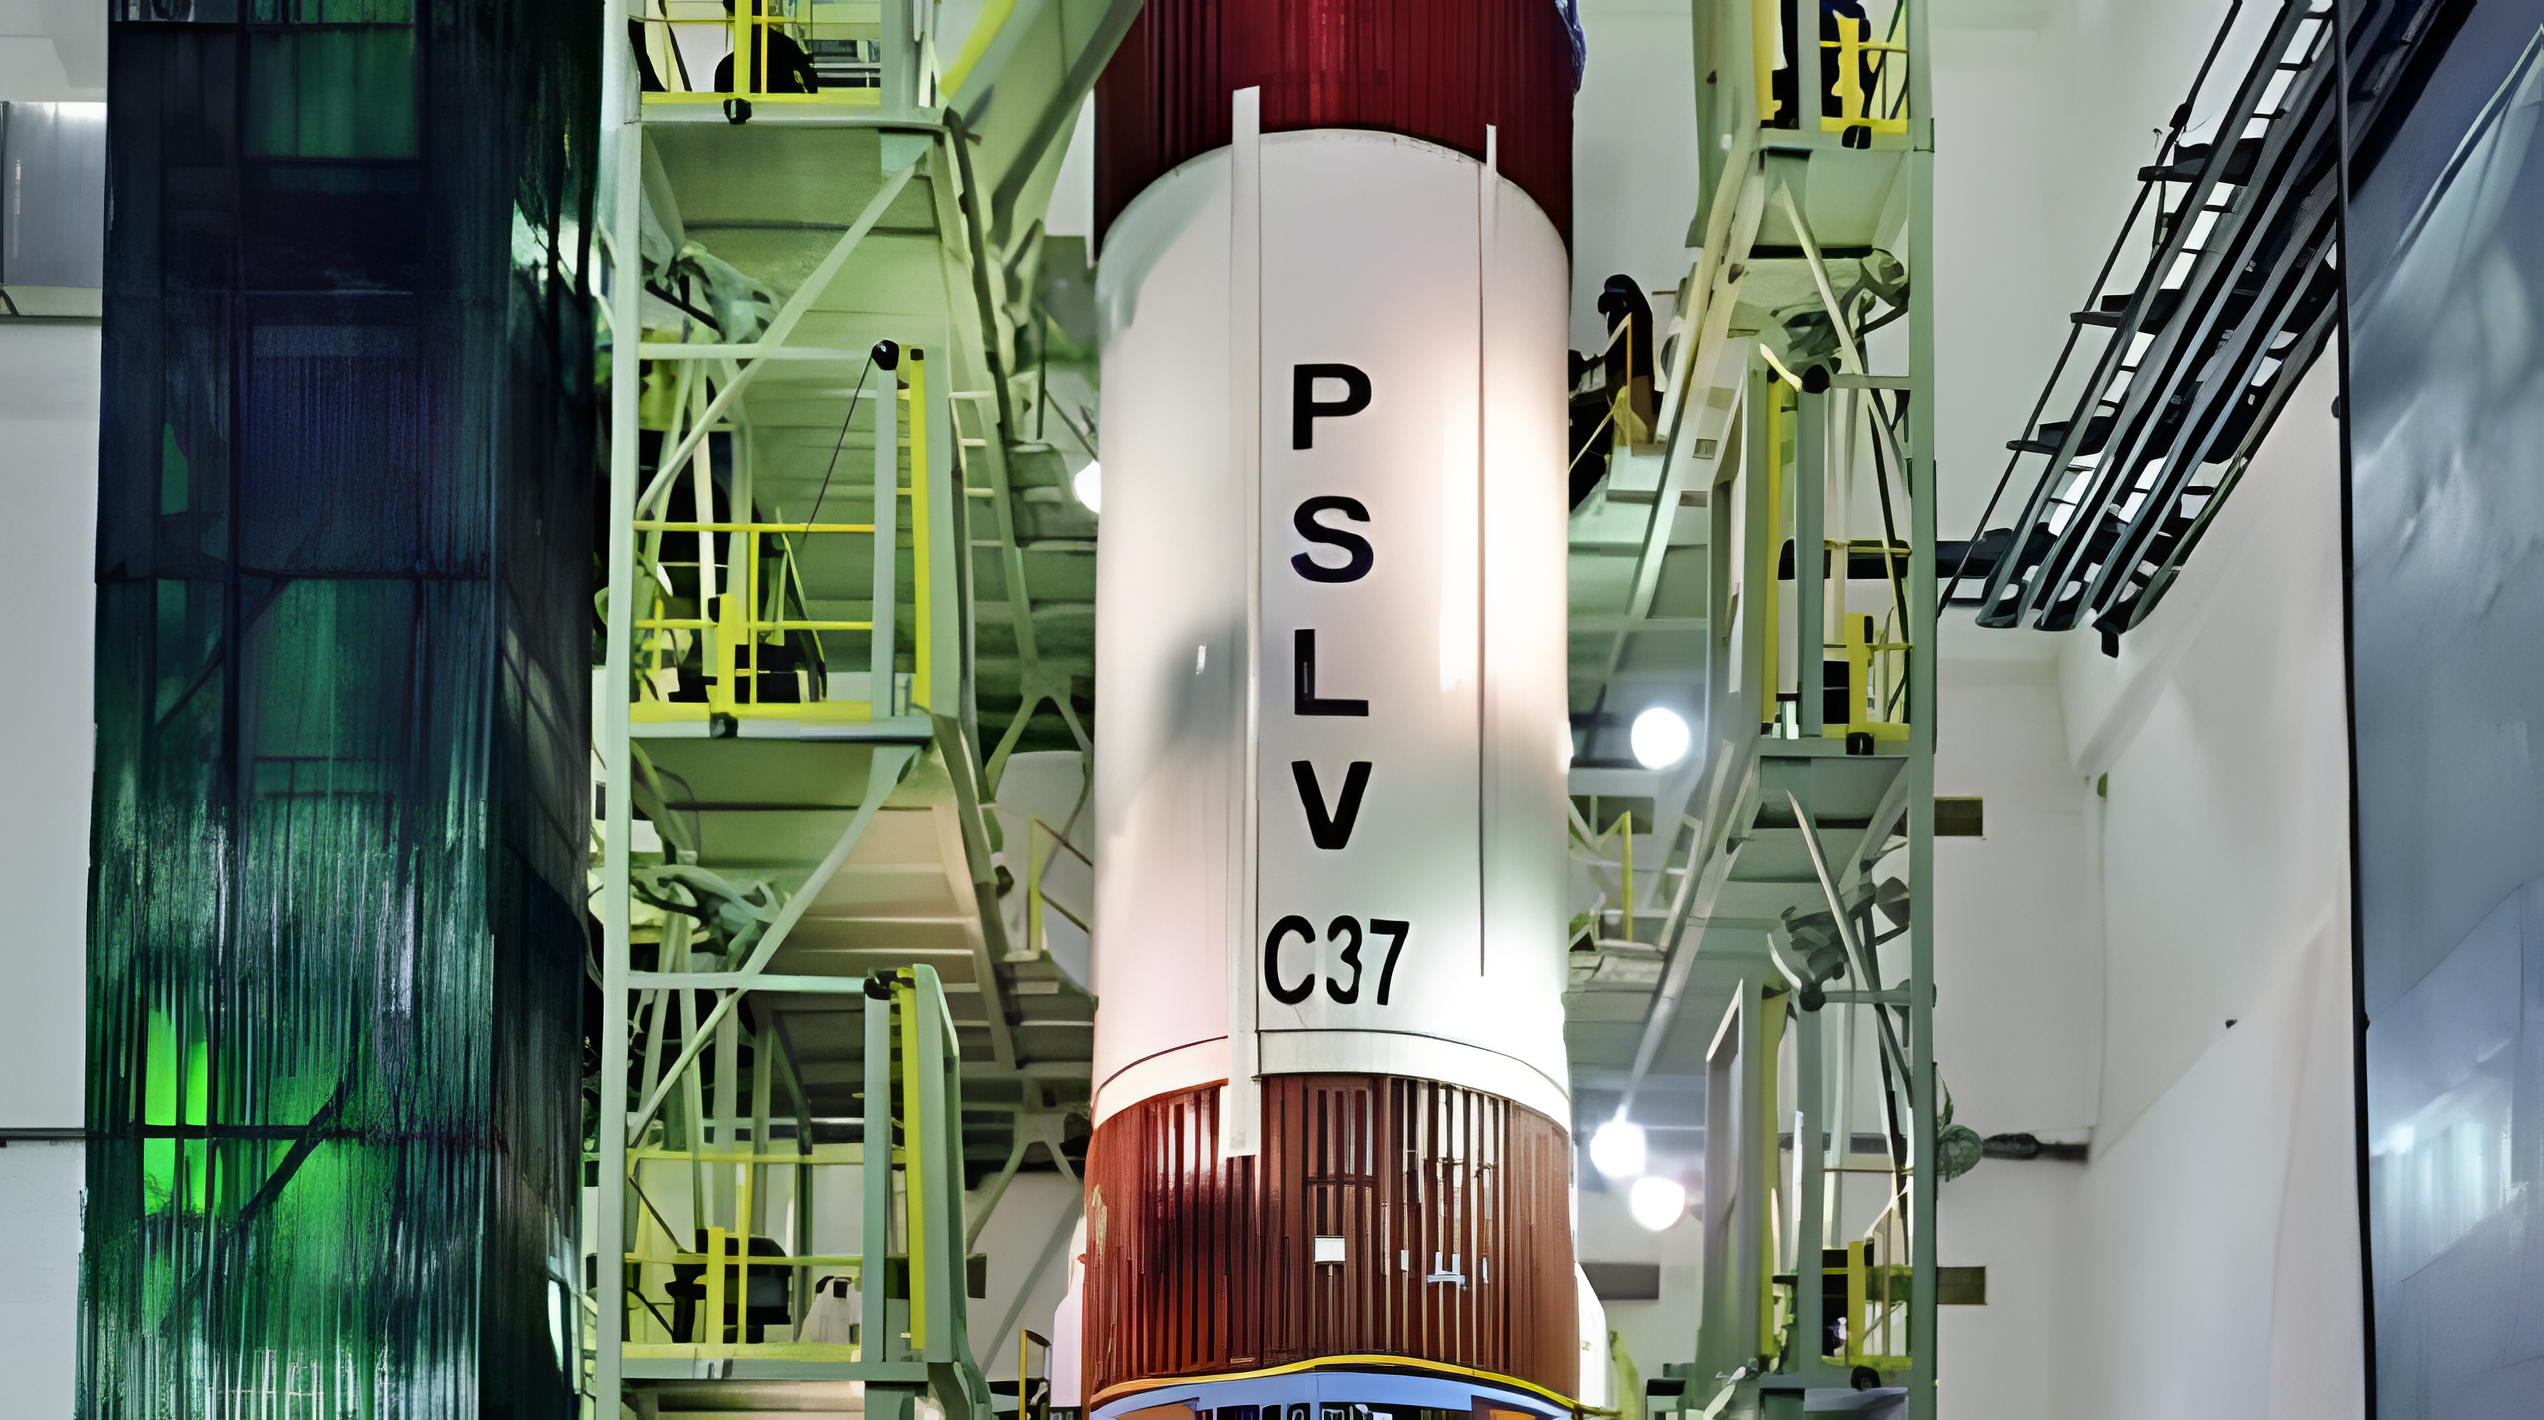
\includegraphics[width=0.85\columnwidth]{assets/images/PSLV.png}
    \vspace{-0.3em}
    \captionof{figure}{PSLV-C37[16] was an historic mission launched by the Indian Space Research Organisation (ISRO) on February 15,
      2017. It successfully deployed a record-breaking 104 satellites in a single rocket flight, which set a global record for the most
    satellites launched in one mission at the time}
\end{minipage}
  \end{center}
\vspace{-0.9em}

  Government agencies previously used to depend on slow and expensive ground surveys. Now days the
  data obtained from satellite are used for land mapping, environmental protection, and infrastructure
  planning work. It not only reduces timeline dramatically, but also provide a improved result. Altogether
  these applications illustrate how ISRO became important for every Indian in day-to-day life. Launch
  records and planetary missions attract attention, but deeper contribution lies in agriculture, natural
  disaster response, fisheries which rarely makes to headlines.

  \subsection*{\centering\uppercase{WEATHER FORECASTING AND DISASTER MANAGEMENT}}
  India is highly vulnerable to wise range of disaster and natural calamities. Cyclone destroy the
  coastlines, floods swallow river plains, droughts stretch across the interior. ISRO's satellite systems
  provide accurate, timely information which is required to prevent catastrophe. Weather data from
  ISRO's satellite is fed directly to early warning systems which give coastal authorities, coast guards
  enough lead time to evacuate people before cyclones make landfall. This capability alone has
  measurably reduced casualties over the past two decades. Satellite imaging-based flood monitoring
  helped disaster management teams to respond affected areas quickly rather than waiting for ground
  reports.

  \begin{center}
\vspace{-0.5em}
\begin{minipage}{0.98\columnwidth}
\centering
    \vspace{-0.2em}
    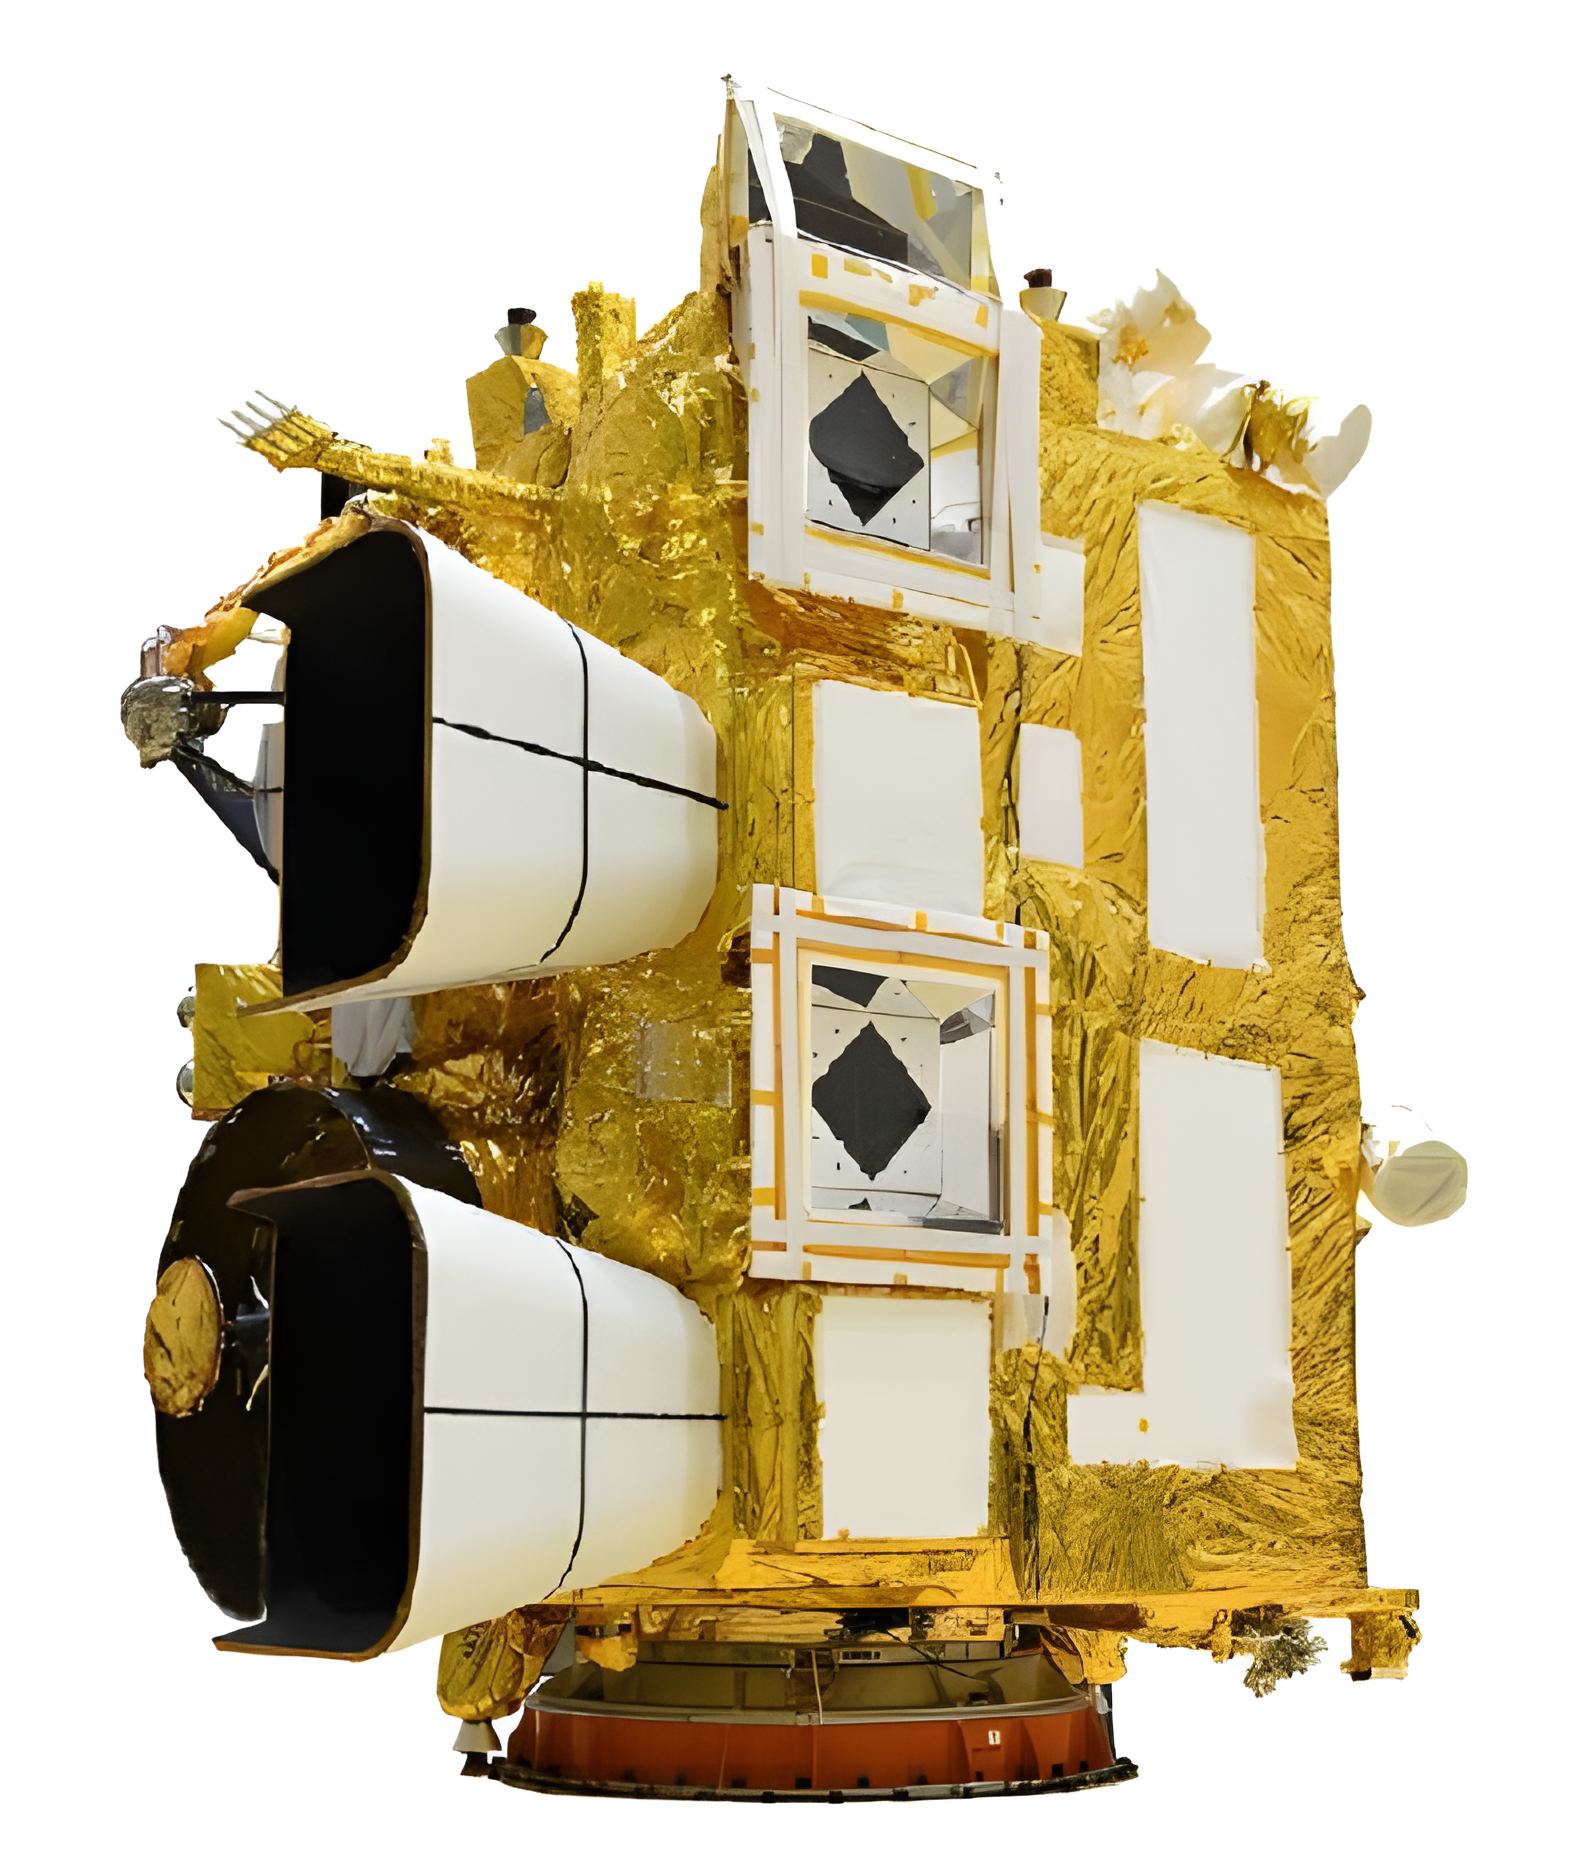
\includegraphics[width=0.75\columnwidth]{assets/images/INSAT.png}
    \captionof{figure}{INSAT-3DS[17] is an advanced meteorological and oceanic observation satellite launched by ISRO on February 17,
      2024. Fully funded by the Ministry of Earth Sciences (MoES), it serves as a follow-up mission to INSAT-3DR[18] and INSAT-
    3D[19]. The satellite enhances India's weather forecasting, climate monitoring, and disaster warning capabilities}
    \vspace{-0.4em}
\end{minipage}
  \end{center}
  \vspace{-0.3em}
  The most significant part isn’t the technology it’s the impact. Space infrastructure is built and operated
  thousands of kilometres above the earth surface. This infrastructure is actively protecting lives in fishing
  villages, river deltas, and hill and mountain region across India. This is how space research contributes
  to human welfare and is more important than any planetary mission.

  \subsection*{\centering\uppercase{NAVIGATION SYSTEMS AND NATIONAL SECURITY}}
  Another technological advancement for ISRO is the development of Navigation with Indian
  Constellation (NavIC). NavIC is India's regional navigation system just like GPS. It provides accurate
  positioning and timing services. The system reduces India's dependence on foreign navigation systems
  like GPS and strengthens technological self-reliance.
  \par\noindent
  NavIC consists of set of seven satellites which includes IRNSS-1A, IRNSS-1B, IRNSS-1C, IRNSS-
  1D, IRNSS-1E, IRNSS-1F, and IRNSS-1G. The system covers India and a region which extends up to
  1500 km beyond the border. NavIC has been implemented in transportation, maritime navigation,
  disaster management and defence purpose due to its precise and reliable data. With advancement in AI
  and drone tech accurate navigation systems are essential for national security and defence purposes.
  During emergencies and strategic operations, NavIC ensures reliable communication and positioning
  services. It played an crucial role in Operation Sindoor and India Pak War.

  \begin{center}
\vspace{-0.5em}
\begin{minipage}{0.98\columnwidth}
\centering
    \vspace{-0.4em}
    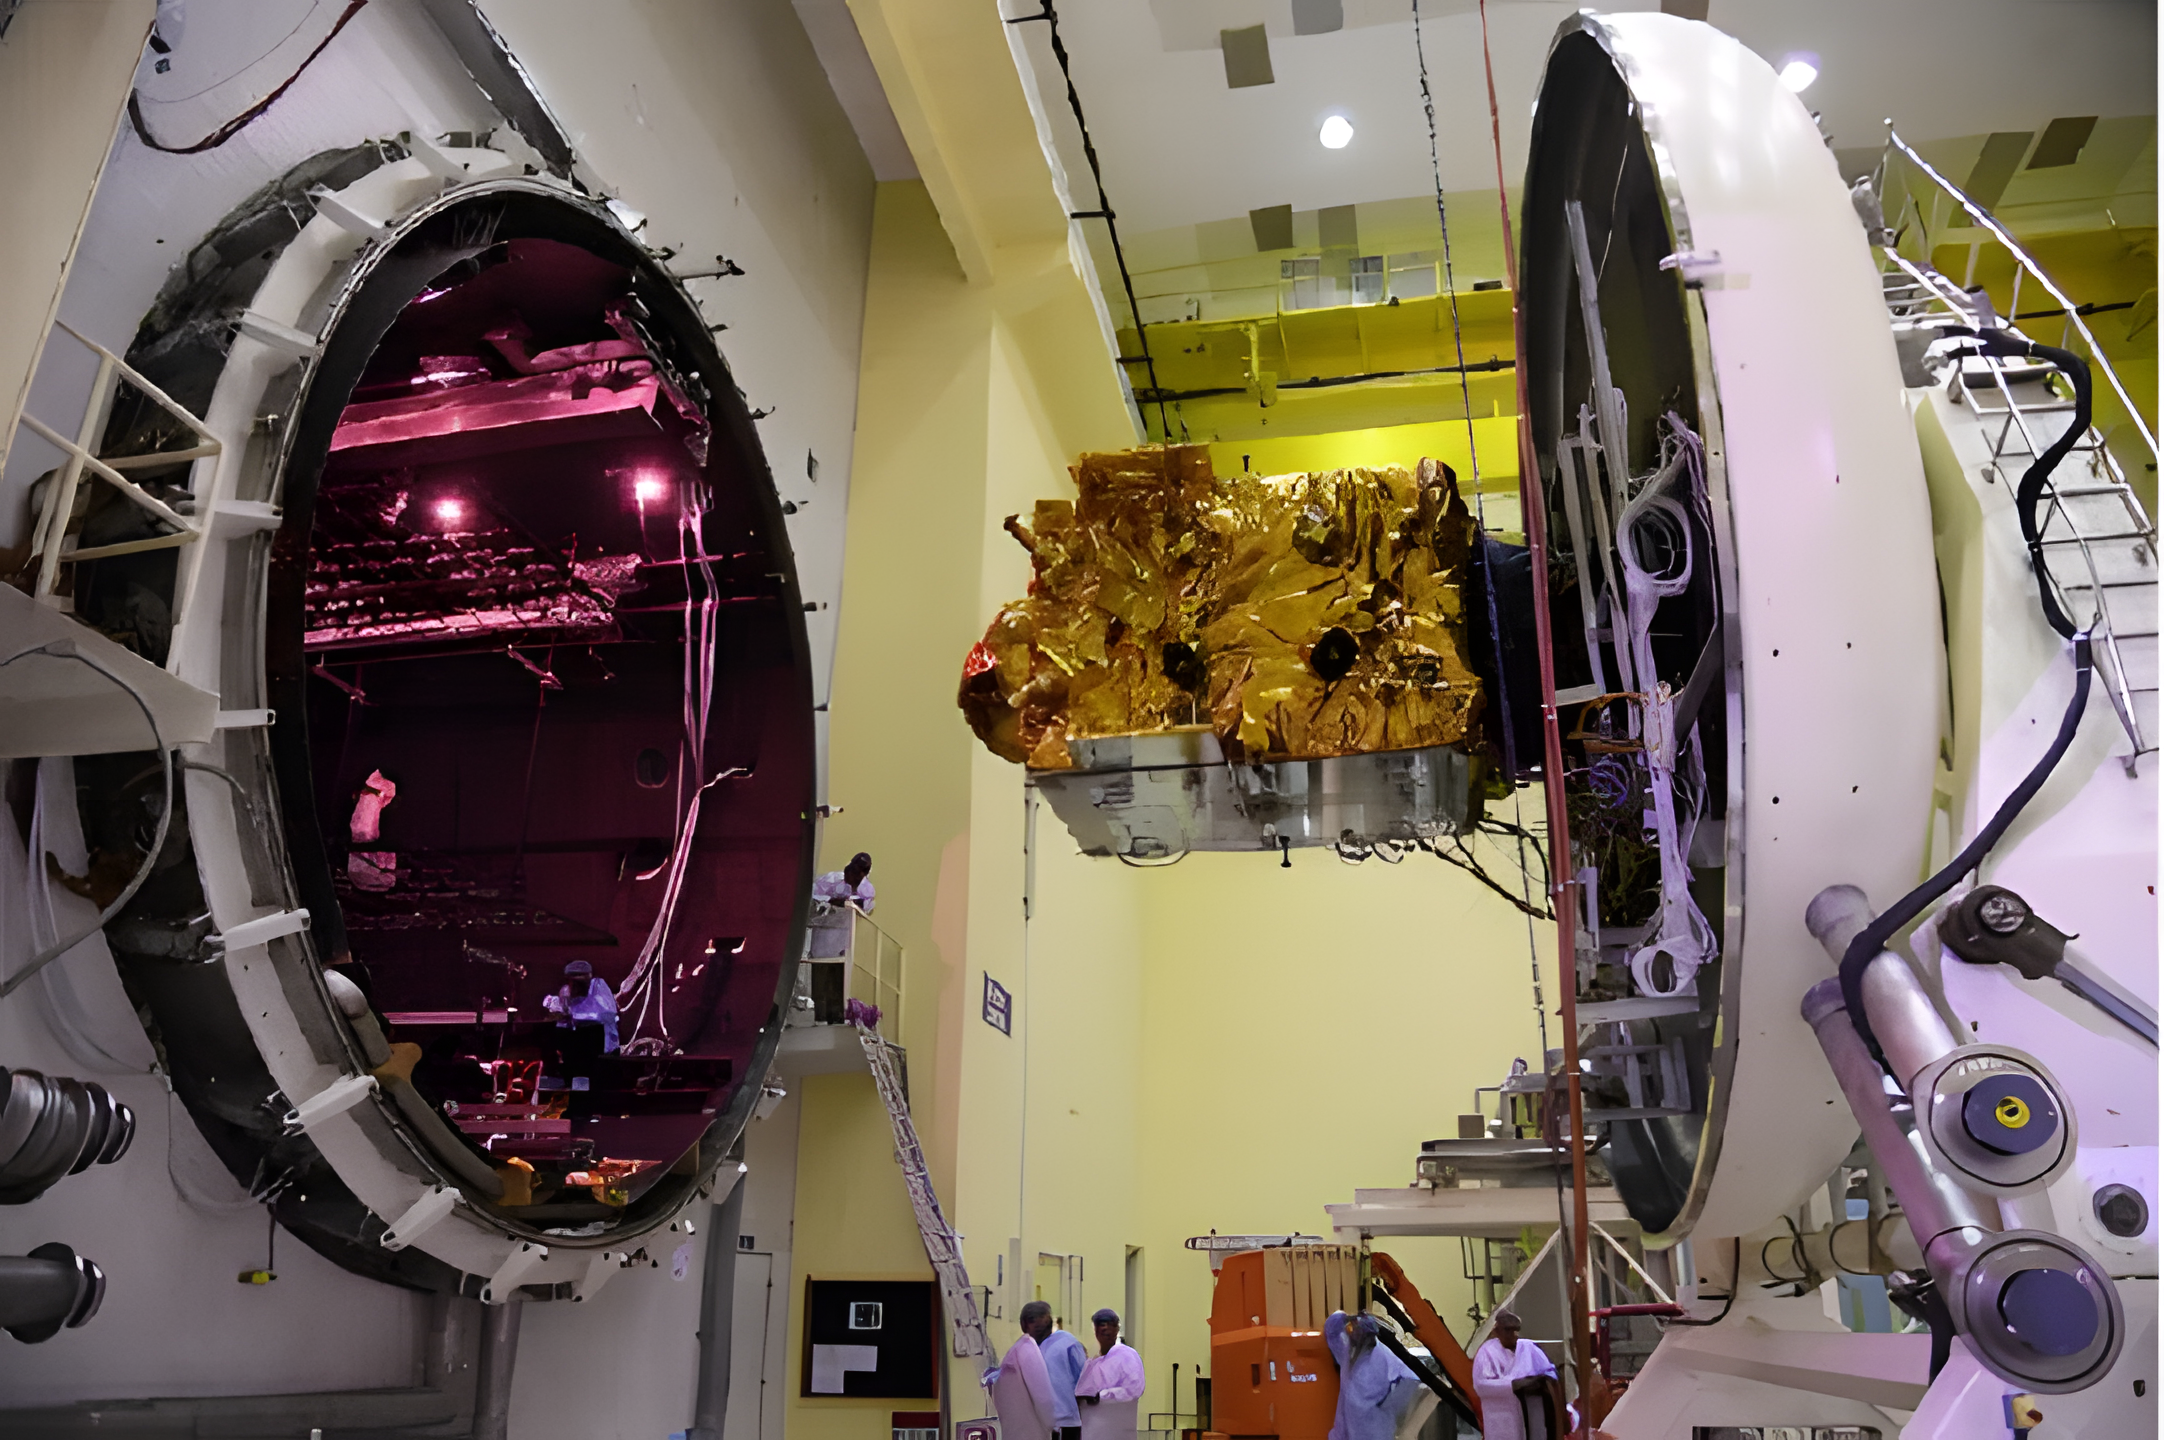
\includegraphics[width=0.75\columnwidth]{assets/images/NavIC.png}
    \captionof{figure}{NavIC (Navigation with Indian Constellation) is India's indigenous regional satellite navigation system developed by
      ISRO. It provides highly accurate real-time positioning, velocity, and timing services across the Indian landmass and up
    to 1,500 km beyond its borders, functioning as a localized, independent alternative to GPS.}
    \vspace{-0.6em}
\end{minipage}
  \end{center}
  \vspace{-0.5em}
  ISRO has also contributed to national security through surveillance satellites and communication
  systems. These technologies support border monitoring, defense operations, and intelligence gathering.
  They strengthen India's security infrastructure.

  \subsection*{\centering\uppercase{MAJOR SPACE MISSIONS}}
  ISRO's mission record proves the organisation’s ability and capability to achieve successful results
  despite limited resources and funding. Chandrayaan-1, India’s first lunar mission launched in 2008
  found evidence of water molecules on the lunar surface. The discovery urprised the international
  scientific and scholar community and questioned traditional thinking about the Moon's history.
  Chandrayaan-2[20] successor of that program failed in the terminal phase when landing during landing
  on south pole. Chandrayaan-3[21] achieved a soft landing near the Moon's south pole, making India
  the fourth country to land on moon. The south is important in scientist community because it is where
  the trapped ice is expected

  \begin{center}
\vspace{-0.5em}
\begin{minipage}{0.98\columnwidth}
\centering
    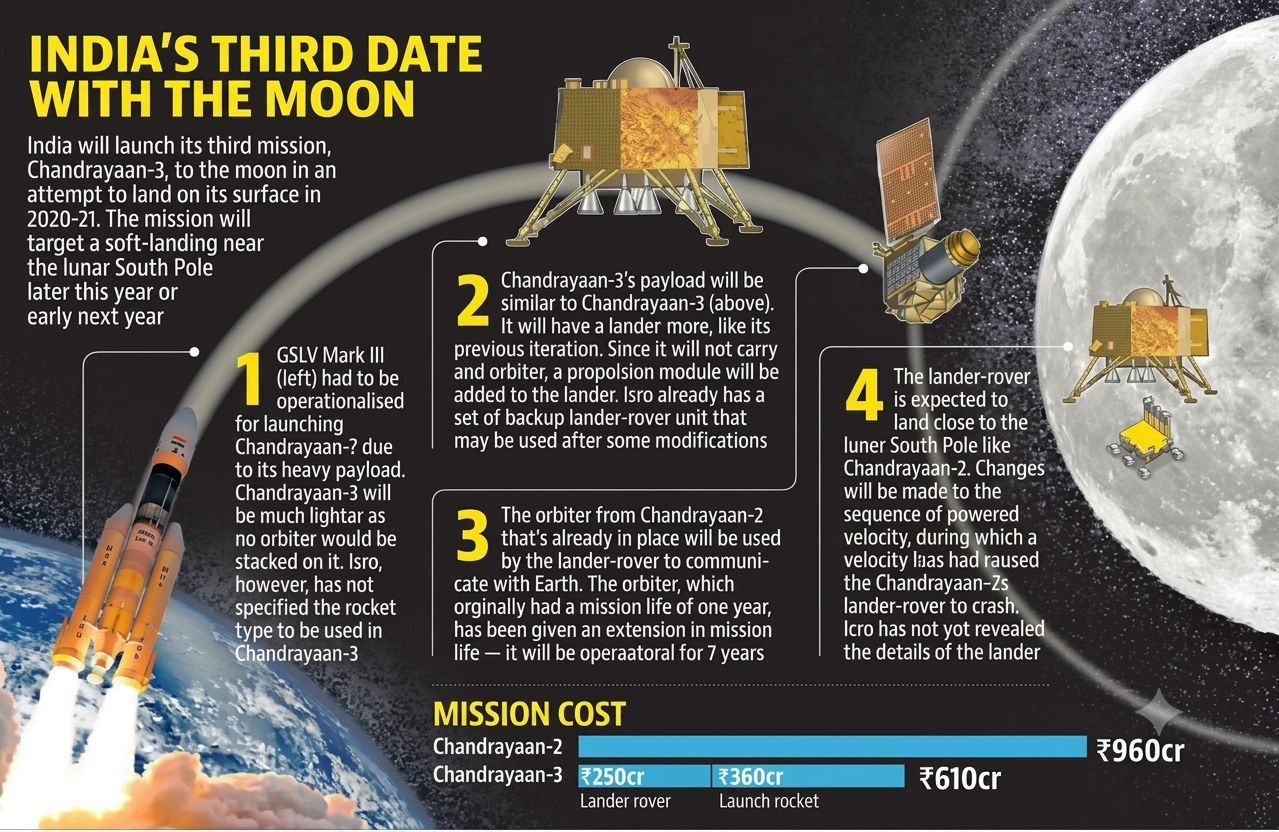
\includegraphics[width=0.8\columnwidth]{assets/images/ITD.png}
    \captionof{figure}{India's Chandrayaan program is a series of lunar exploration missions developed by the Indian Space Research Organisation
      (ISRO). It began in 2008 with Chandrayaan-1, an orbiter mission that famously discovered water on the Moon. This was followed
      by Chandrayaan-2 in 2019, which successfully deployed an orbiter but suffered a lander crash. Chandrayaan-3 successfully
    achieved a historic soft landing at the lunar south pole in 2023.}
\end{minipage}
  \end{center}

  Mangalyaan arrived at Mars in 2014 on India's first attempt at a budget almost half of Interstellar
  movie. The engineering was elegant, the budget was tight, and it worked.

  \begin{center}
\vspace{-0.5em}
\begin{minipage}{0.98\columnwidth}
\centering
    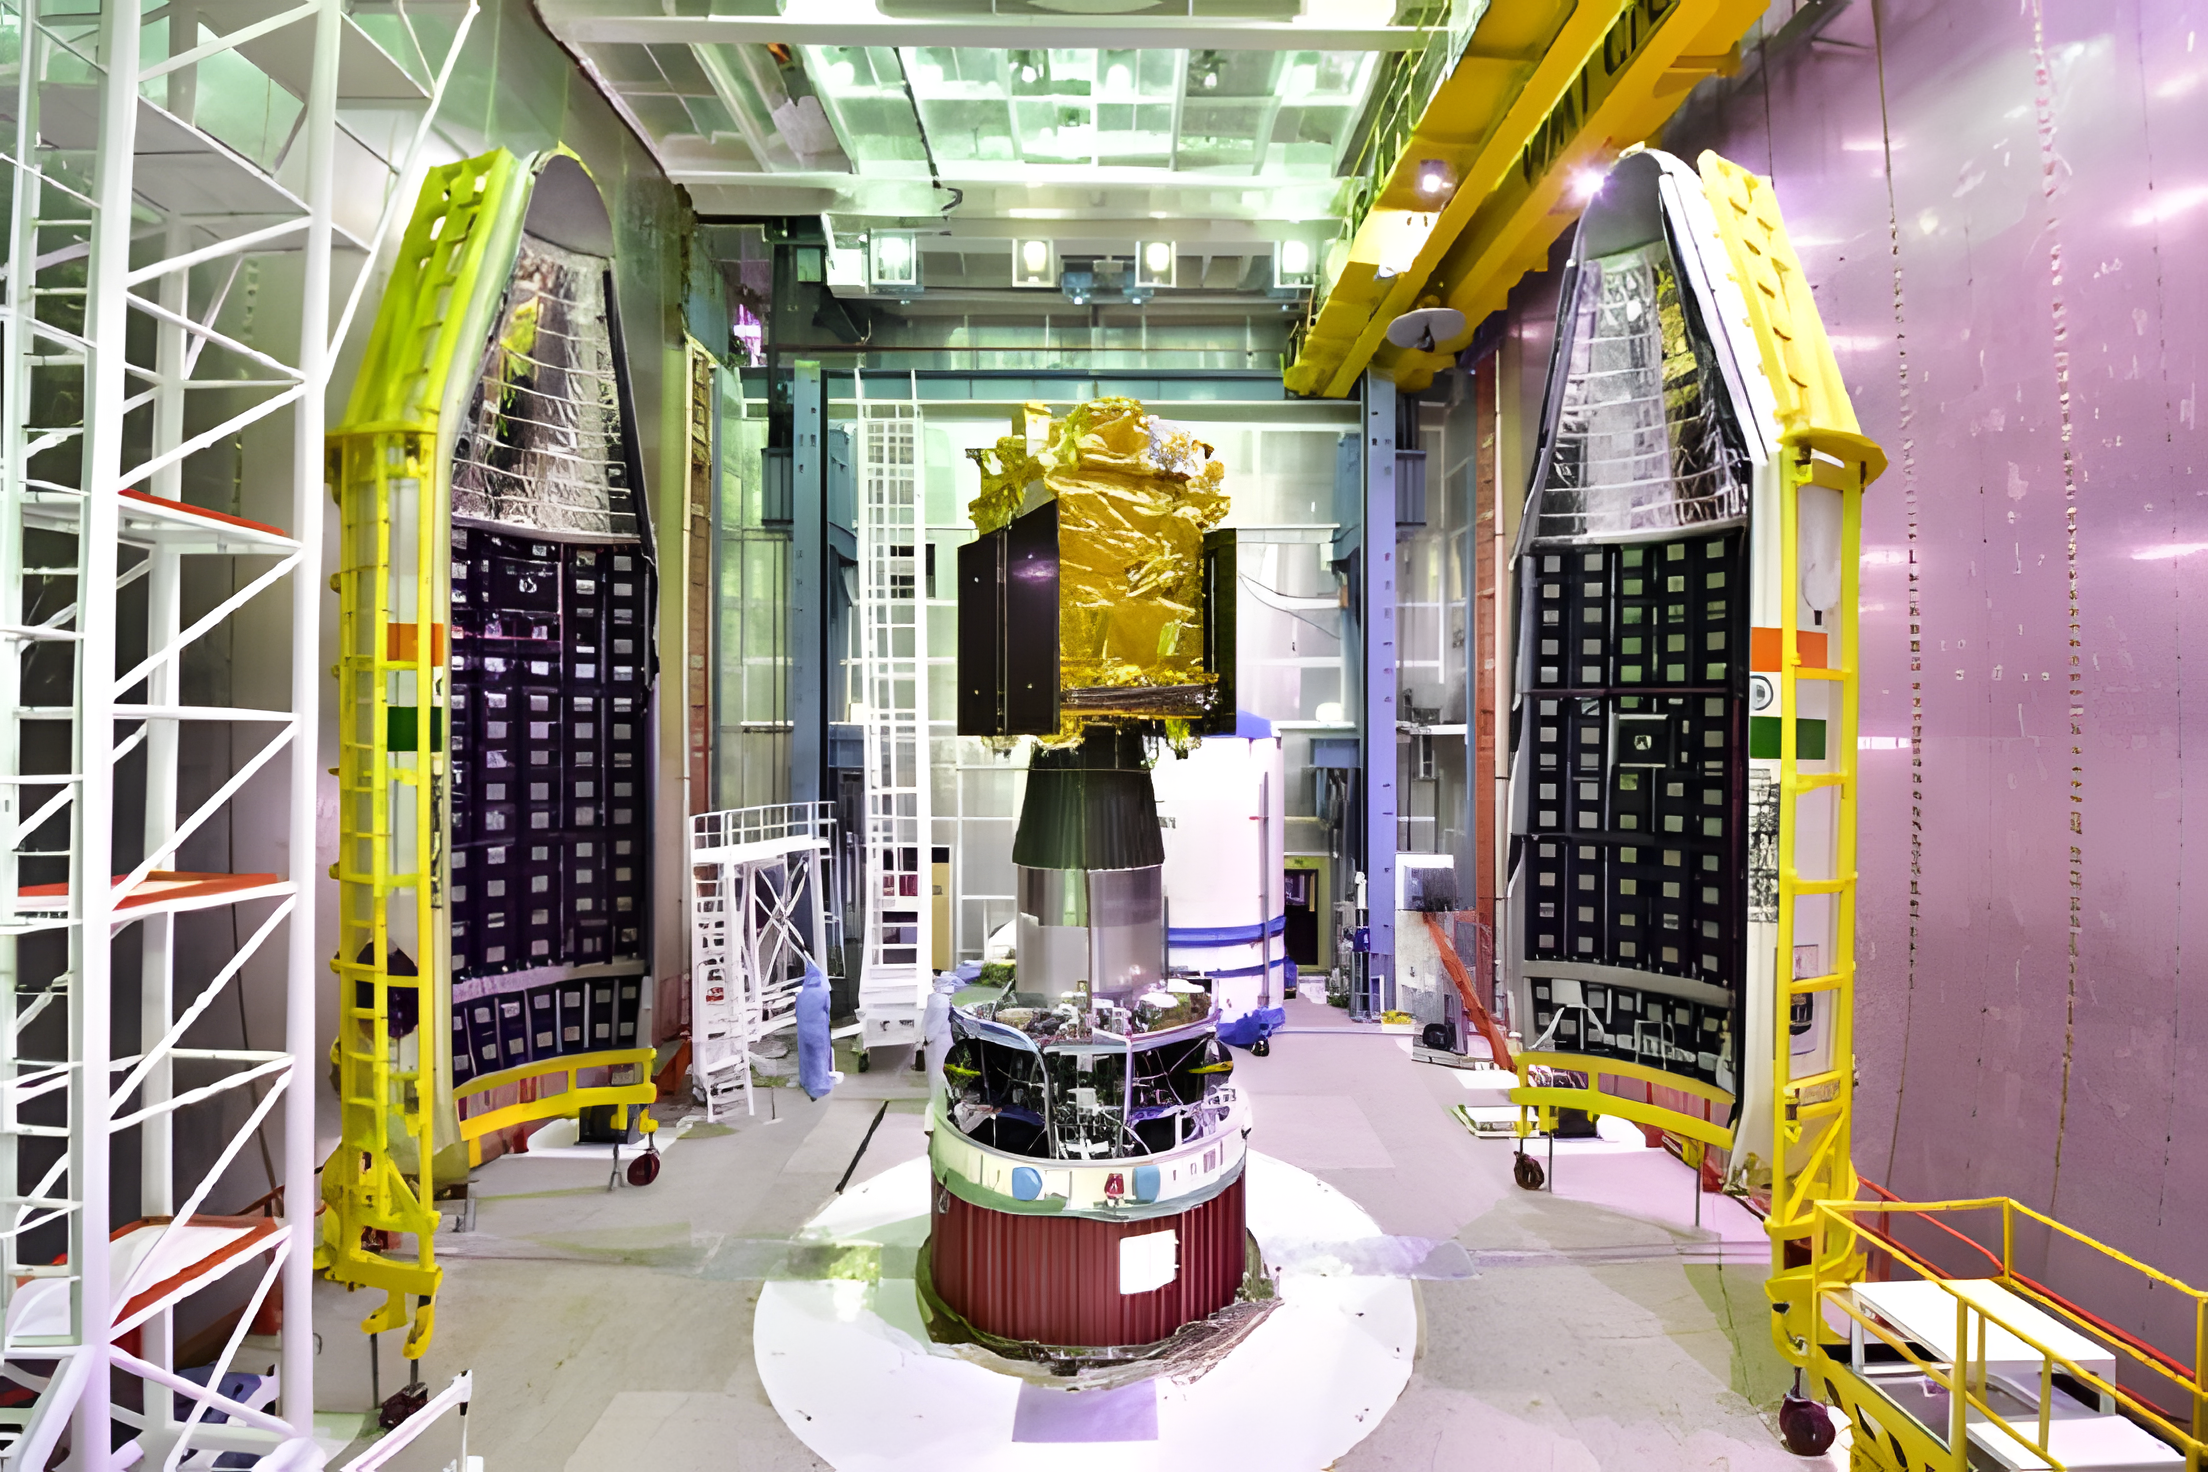
\includegraphics[width=0.65\columnwidth]{assets/images/MOM.png}
    \captionof{figure}{Mangalyaan, officially known as the Mars Orbiter Mission (MOM), is the Indian Space Research Organisation’s (ISRO)
      Mars Orbiter Mission - ISRO maiden interplanetary space probe. Launched on November 5, 2013, it successfully entered Martian
    orbit on September 24, 2014, making India the first nation to achieve this in its first attempt}
\end{minipage}
  \end{center}
\vspace{-0.4em}

  Aditya-L1, now stationed at the Sun-Earth L1 point, is used to study solar activity and space weather.
  It is highly important as all satellite infrastructure are highly vulnerable to solar events. Gaganyaan
  India's first crewed mission is the upcoming project. If it succeeded it would place India would be the
  fourth country in the world to have sent humans to space independently. The bar is extremely high as
  any single fault would cost human lives .ISRO is conducting exhaustive testing to master the
  technology

  \begin{center}
    \begin{minipage}{\columnwidth}
    \centering
    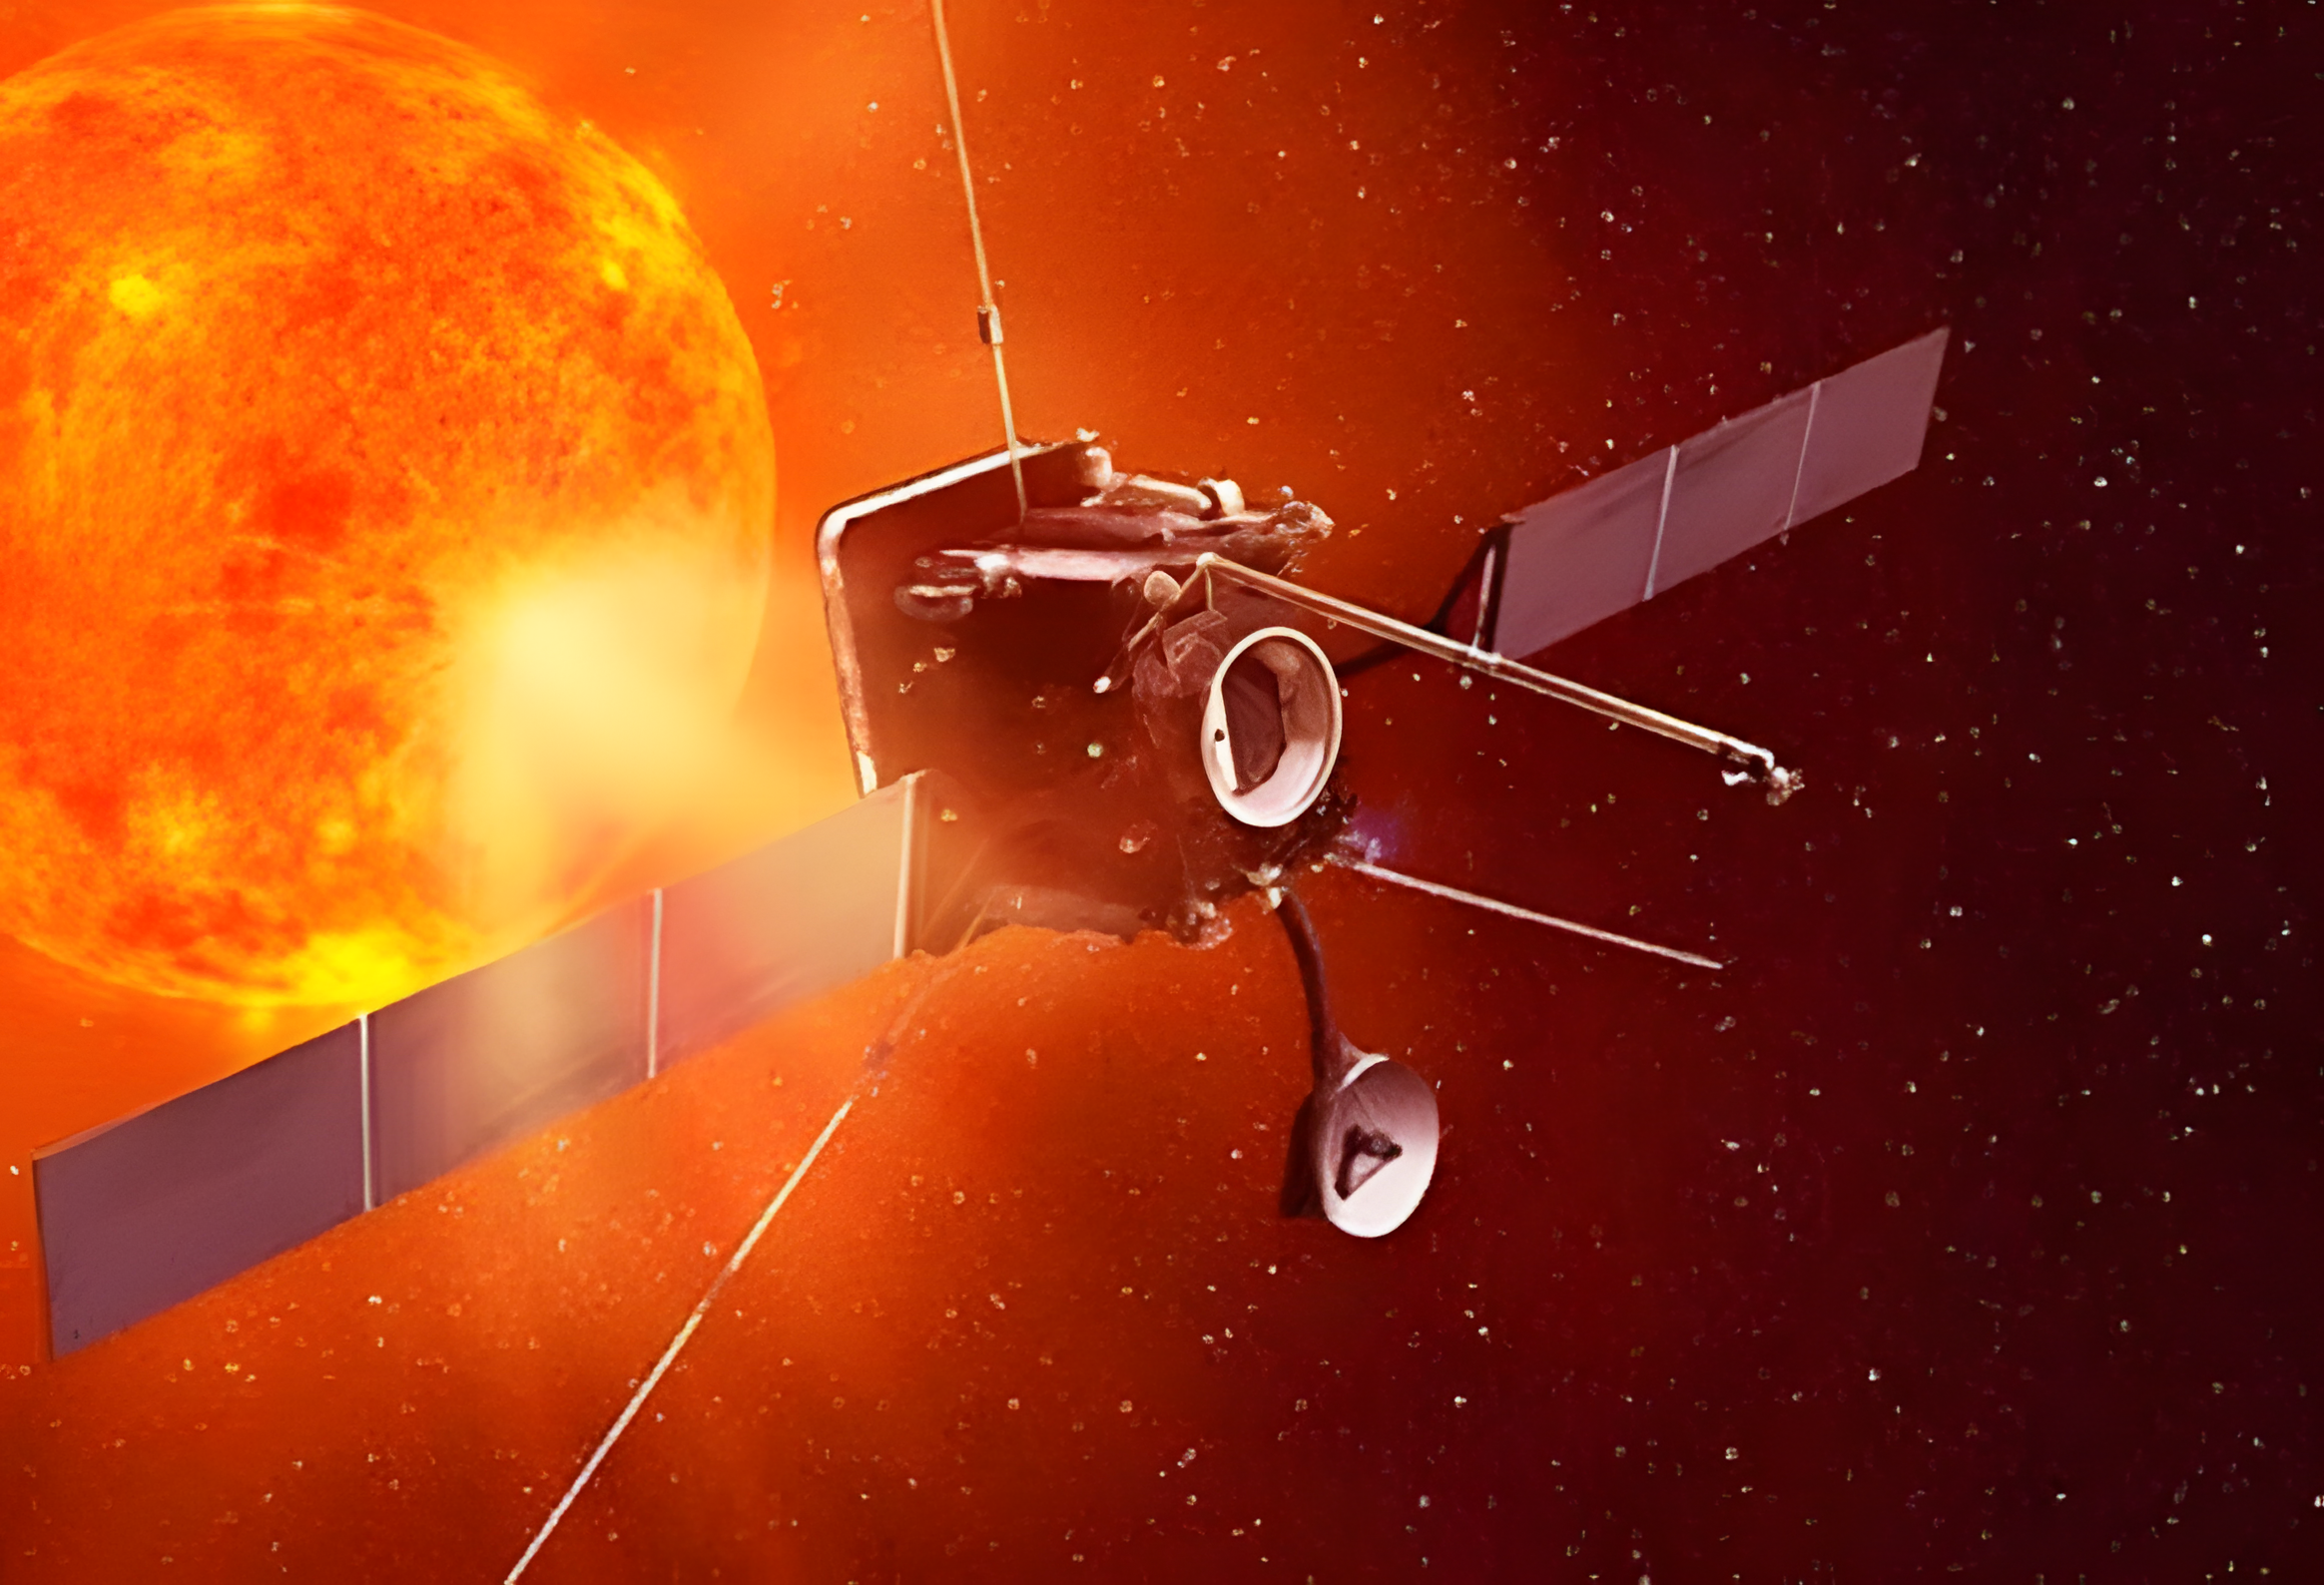
\includegraphics[width=0.85\columnwidth]{assets/images/AL1.png}
    \captionof{figure}{Aditya-L1, India’s first dedicated solar observatory, studies the Sun and space weather from the Sun--Earth L1 point.}
    \end{minipage}
  \end{center}
  \subsection*{\centering ISRO'S CONTRIBUTION TO SCIENCE, EDUCATION, AND INDUSTRY}
  The achievements of the Indian Space Research Organisation (ISRO) have boosted interest and
  curiosity in science and technology among Indians. Watching Mangalyaan reaching Martian orbit and
  Chandrayaan soft landing on south pole have inspired many Indian students to pursue their future
  studies in science and engineering. As a result, fields such as aerospace engineering, robotics, and
  artificial intelligence, once considered unattainable, and distant are now attracting a large number of
  students every year. ISRO collaborates with universities and research institutions to provide
  internships and training opportunities, providing a platform for students to link academic interests
  with practical real world engineering problems. Private enterprises are also increasingly involved in
  space exploration, contributing so rapidly to satellite technology, launch vehicle development, and
  space research that a single government agency cannot keep up.

  \begin{center}
    \begin{minipage}{\columnwidth}
    \centering
    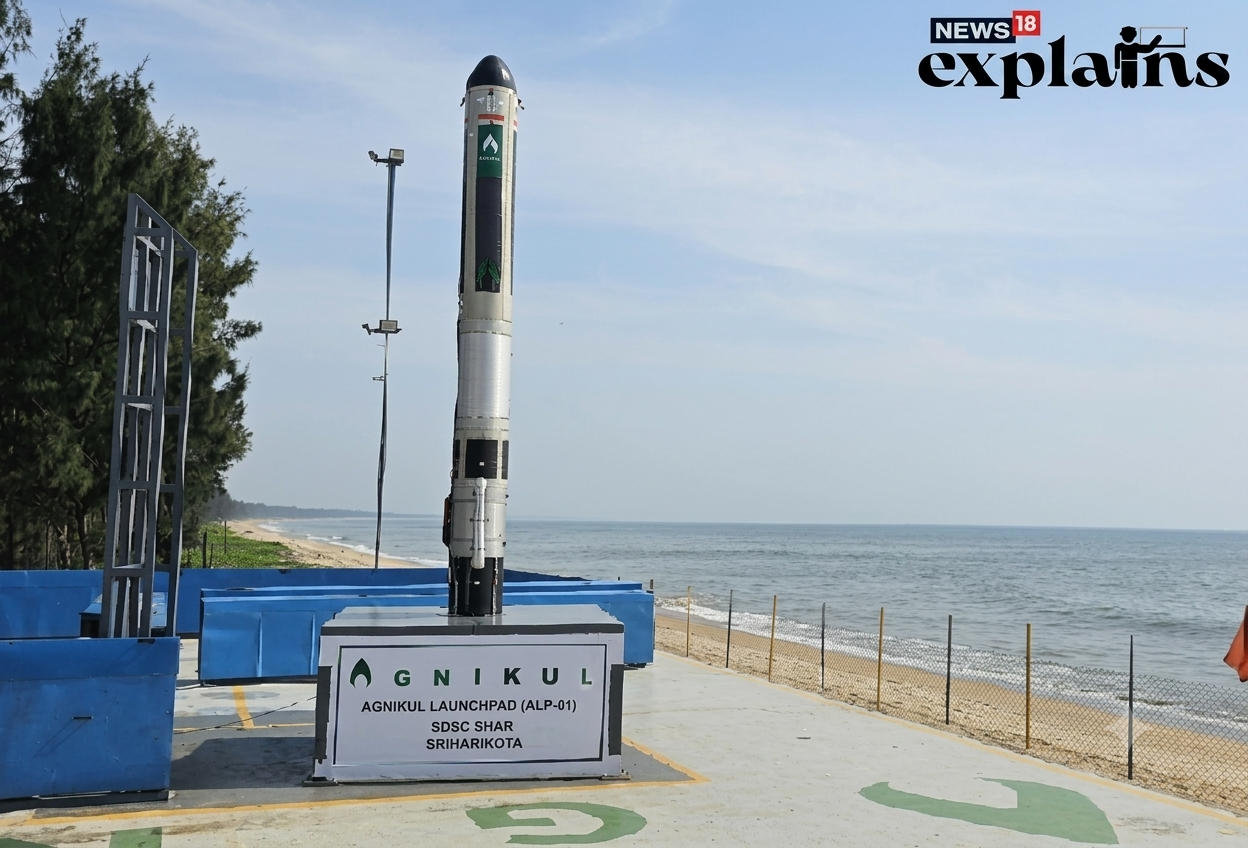
\includegraphics[width=0.85\columnwidth]{assets/images/IITM.png}
    \captionof{figure}{Agnikul Cosmos, an IIT Madras-incubated startup, successfully launched the Agnibaan SOrTeD[22] (Sub-Orbital
      Technology Demonstrator) rocket from Sriharikota, powered by the world's first single-piece 3D-printed semi-cryogenic
    engine. The historic flight validated the startup's in-house 3D printing and software-defined propulsion technologies.}
    \end{minipage}
  \end{center}

  Today the shift from single government agency ISRO to multiple private companies have joined and
  honestly it created more jobs and money . Engineers from startups like Skyroot and Agnikul are us who
  grew up watching from a young age what ISRO has pulled off despite having limited resources or
  funding. As government is pushing towards commercialisation, scientist or engineers who would have
  previously left for NASA or ESA are now staying back in India. But honestly if rockets and satellite are
  kept aside, they have created a sense of culture. It showed what Indian scientists what they are actually
  capable to pull off when system or politics don’t intervene. For a kid who is confused about their career;
  watching ISRO succeed from childhood , makes them feel certain career are actually achievable no
  matter how hard they are. This actually matters more than any policy

  \subsection*{\centering\uppercase{FUTURE PROSPECTS AND CHALLENGES}}
  The future direction is indeed ambitious: reusable rockets, longer-distance space missions, advanced
  satellites—India even once hoped to have its own domestically built space station. Several projects have
  begun development and are no longer just on paper. The challenges are real. The emergence of SpaceX
  has intensified global competition and changed expectations about launch costs. Space debris[23] is no
  longer just a theoretical problem but has become a practical challenge. Satellite infrastructure is facing
  more cybersecurity[24] threats. How to reduce costs while pushing the limits of technology has now
  become a real challenge.

  \par\noindent
  Frankly, the Indian Space Research Organisation (ISRO)'s greatest strength lies in its tangible
  achievements. The successful first Mars landing, the reliable and stable NavIC navigation satellite
  system developed in-house, and its relentless pursuit of innovation—these are no accident; ISRO has
  found viable solutions and persisted in using them in every attempt. The challenges of the future are
  vastly different from those of fifty years ago, but what truly matters remains unchanged. Space is
  becoming central to India's future development. ISRO started almost from scratch. Frankly, there's no
  reason to believe they will stop here.

  \subsection*{\centering\uppercase{CONCLUSION}}
  The story of the Indian Space Research Organisation (ISRO) is an unbelievable tale on how to stretch
  every rupee to its absolute limit, surpassing every person expectation. For over fifty years, they have
  established communication networks, navigation systems, weather forecasting capabilities, and disaster
  warning systems. ISRO have accomplished all this with tight budget and limited resources guided by
  clear and well-defined priorities. Their flagship missions have earned attention worldwide: the
  *Chandrayaan* lunar probe confirmed the presence of water on the Moon; Mangalyaan the *Mars
  Orbiter Mission* successfully reached Mars on its very first attempt; and the *Aditya-L1* probe
  propelled India into the realm of solar physics; fields only a handful of agencies have actually acquired.
  Moreover the underrated efforts such as NavIC system, which reduces reliance on foreign GPS, and
  remote sensing where satellites are used to provide data support for agricultural and environmental
  decision-making likely impact the lives of millions of Indians on a daily basis.
  The future developments of ISRO are equally significant. Gaganyan mission will place India among
  the list of very few countries capable of conducting human spaceflight independently. Deep space
  exploration[25] are beginning to take shape.The growing enterprise of private startups, university
  collaborations, and commercial launches surrounding the Indian Space Research Organisation (ISRO)
  will further accelerate all of this. For India, space technology and national development have never been
  separate goals. ISRO has integrated the two, and this foundation appears solid enough to support
  significant future growth.

  \subsection*{\centering\uppercase{References}}
  \begingroup\justifying
  \Urlmuskip=0mu plus 1mu\relax
  \begin{enumerate}[leftmargin=*,itemsep=0.20em,topsep=0.12em,parsep=0pt]
    \item National Air and Space Museum, “All About Rockets.” [Online]. Available:
      \url{https://airandspace.si.edu/learn/programs/soar-together/rockets-2}.
    \item Indian Space Research Organisation, “Chandrayaan-1.” [Online]. Available:
      \url{https://www.isro.gov.in/Chandrayaan_1.html}.
    \item Indian Space Research Organisation, “Aditya-L1.” [Online]. Available:
      \url{https://www.isro.gov.in/Aditya_L1.html}.
    \item National Aeronautics and Space Administration, “What is a Lagrange Point?” [Online]. Available:
      \url{https://science.nasa.gov/resource/what-is-a-lagrange-point/}.
    \item National Aeronautics and Space Administration, “NASA Heliophysics.” [Online]. Available:
      \url{https://science.nasa.gov/heliophysics/}.
    \item Indian Space Research Organisation, “Satellite Navigation Services.” [Online]. Available:
      \url{https://www.isro.gov.in/SatelliteNavigationServices.html}.
    \item Wikipedia, “Skyroot Aerospace.” [Online]. Available:
      \url{https://en.wikipedia.org/wiki/Skyroot_Aerospace}.
    \item Wikipedia, “Agnikul Cosmos.” [Online]. Available:
      \url{https://en.wikipedia.org/wiki/AgniKul_Cosmos}.
    \item Indian Space Research Organisation, “Gaganyaan.” [Online]. Available:
      \url{https://www.isro.gov.in/Gaganyaan.html}.
    \item Indian Space Research Organisation, “Dr. Vikram Ambalal Sarabhai (1963–1971).” [Online].
      Available: \url{https://www.isro.gov.in/sarabhaiformer.html}.
    \item EverybodyWiki, “C. R. Sathya.” [Online]. Available:
      \url{https://en.everybodywiki.com/C._R._Sathya}.
    \item President of India, “Dr. APJ Abdul Kalam Profile.” [Online]. Available:
      \url{https://presidentofindia.nic.in/dr-apj-abdul-kalam-profile}.
    \item Indian Space Research Organisation, “Aryabhata.” [Online]. Available:
      \url{https://www.isro.gov.in/aryabhata_1.html}.
    \item Indian Space Research Organisation, “PSLV.” [Online]. Available:
      \url{https://www.isro.gov.in/PSLV_CON.html}.
    \item Indian Space Research Organisation, “Geosynchronous Satellite Launch Vehicle Mark II.”
      [Online]. Available: \url{https://www.isro.gov.in/GSLV_CON.html}.
    \item Indian Space Research Organisation, “PSLV-C37 / Cartosat-2 Series Satellite.” [Online].
      Available: \url{https://www.isro.gov.in/mission_PSLV_C37.html}.
    \item Indian Space Research Organisation, “INSAT-3DS Meteorological and Oceanographic Satellite.”
      [Online]. Available: \url{https://www.mosdac.gov.in/insat-3ds}.
    \item Indian Space Research Organisation, “INSAT-3DR.” [Online]. Available:
      \url{https://www.isro.gov.in/INSAT_3DR.html}.
    \item MOSDAC, “INSAT-3D.” [Online]. Available: \url{https://www.mosdac.gov.in/insat-3d}.
    \item Indian Space Research Organisation, “Chandrayaan-2.” [Online]. Available:
      \url{https://www.isro.gov.in/Chandrayaan_2.html}.
    \item Indian Space Research Organisation, “Chandrayaan-3 Details.” [Online]. Available:
      \url{https://www.isro.gov.in/Chandrayaan3_Details.html}.
    \item PMF IAS, “Agnibaan Sub-Orbital Technology Demonstrator (SOrTeD).” [Online]. Available:
      \url{https://www.pmfias.com/agnibaan-suborbital-technology-demonstrator-sorted/}.
    \item European Space Agency, “About Space Debris.” [Online]. Available:
      \url{https://www.esa.int/Space_Safety/Space_Debris/About_space_debris}.
    \item Kaspersky, “What is Cyber Security?” [Online]. Available:
      \url{https://www.kaspersky.com/resource-center/definitions/what-is-cyber-security}.
    \item National Aeronautics and Space Administration, “Deep Space Network.” [Online]. Available:
      \url{https://www.nasa.gov/communicating-with-missions/dsn/}.
  \end{enumerate}
  \par\endgroup



\end{multicols}
\endgroup


\begin{center}
\begin{tcolorbox}[colback=SoftBlue, colframe=IEEEblue!70!black, boxrule=0.5pt, arc=0mm, left=3mm, right=3mm, top=2mm, bottom=2mm, width=0.92\textwidth]
\small\RaggedRight \textbf{\color{IEEEblue!75!black}Did you know?} — India's NavIC covers India plus 1,500\,km beyond with just 7 satellites, an independent alternative to GPS.
\end{tcolorbox}
\end{center}

\begin{center}
  \section{\capitalisewords{Artificial Intelligence for Network Security \& Threat Prevention}}
  Priyanka Manna, 3$^{rd}$ Year, ECE
\end{center}

\setcounter{figure}{0}

\begin{multicols}{2}
  \begin{abstract}
    \bfseries
    This analysis analysis the deep influence of artificial intelligence in protecting our digital world. The latest research indicates an event where traditional security protocols are falling behind, but AI, especially machine learning and deep learning, is in place to catch advanced threats such as rogue programs and zero-day attacks before they can do real damage. These studies show that AI isn’t just for big technology; its ability to detect patterns in massive amounts of data in real-time makes it a crucial instrument for everything from protecting a local bank to securing the complex sensors that are used in modern factories and smart cities.

    \noindent
    But the papers also remind us that AI is not a “magic button.” There are real hurdles to clear, like making sure the data used to train these systems is accurate, removing unconscious biases and navigating the tricky ethics of automated security. A common thread throughout this work is the idea of a "synthetic defence,” which is the raw processing power of AI working in conjunction with human intuition and judgment. At the end of the day, we can’t afford to be reactive – cyberattacks are becoming more frequent, and inventive. The decision is to safeguard our data and maintain public trust, we must stay ahead of technology and put these smart frameworks in place, so our digital defences evolve alongside the threats they protect up against.

  \end{abstract}

  \subsection*{\centering\uppercase{INTRODUCTION}}
  With the explosive growth of global cyber threats, traditional signature-based defence mechanisms are becoming more and more irrelevant and have to evolve to more dynamic and intelligent systems of security. The driving forces behind this change have been Artificial Intelligence (AI) and Machine Learning (ML). These technologies have the ability to compute to sift through huge volumes of data and spot unusual patterns instantly. Beyond static rules, these technologies facilitate a transition from reactive models to proactive, predictive defence strategies capable of thwarting sophisticated attacks such as zero-day exploits and polymorphic malicious software. This integration provides a flexible shield for essential infrastructure, ranging from financial networks to Industry 4.0 environments. But as the digital landscape becomes more volatile, AI also brings new complexities, such as hostile attacks and the urgent need for algorithmic transparency. In the end, the future of cybersecurity is a partnership of machine precision and human intuition, a resilient ecosystem able to adapt as quickly as the threats it tries to counter, protecting the integrity and privacy of our more and more interconnected world.

  \subsection*{\centering\uppercase{REVIEW OF RELATED LITERATURE}}
  \subsubsection*{Foundational AI Paradigms in Cybersecurity}
  One of the key threads in recent cybersecurity research has been the move from traditional, signature-based defences, to intelligent, adaptive frameworks. Vyas et al. [3] stated that the main disadvantage of legacy systems is their inability to fight “zero-day” threats and evolving malware signatures. Researchers have contributed to the area of Artificial Intelligence (AI) to make the defence proactive rather than reactive, to address this issue. The core idea is to apply machine learning algorithms over real-time network traffic and user behaviour. Rizvi et al. show that AI can identify subtle anomalies indicative of potential breaches (e.g., unauthorized data leakage or credential harvesting) by training models on large-scale datasets [4]. These early AI-based systems provided substantial improvements in detection rates, but were often dependent on centralized data processing, which resulted in latency and potential single points of failure.

  \subsubsection*{Deep Learning and Algorithmic Advancements}
  With more advanced threats, the literature has migrated towards the use of more advanced deep learning architectures to improve accuracy and reduce false positives. Research presented in IEEE Xplore discusses the application of specialized neural networks like Convolutional Neural Networks (CNNs) and transformer-based models for detection of complex attack patterns in large streams of data [1]. These implementations facilitate automatic feature extraction, without manual security rules. Another major focus has been the use of AI in finance. It is known that AI-based predictive modelling is important for protecting high-value digital transactions against fraud and ransomware [2]. The digital architectures use software-defined thresholds and adaptive learning to constantly revise their detection logic as new threats arise.

  \subsubsection*{Sector-Specific Applications and Emerging Challenges}
  The most recent development is around scaling of AI security into specialized domains such as Industry 4.0 and Internet of Things (IoT). Dhanushkodi et al. [1][5] argue that as industrial environments become more connected, the attack surface is increasing and AI is needed to manage the security of heterogeneous devices. Furthermore, recent researches are also exploring the intersection of AI and decentralization to improve the data integrity and privacy of cloud ecosystem. These breakthroughs notwithstanding, the literature points out that challenges remain, including the high computational cost of training robust models, and the threat of adversarial AI, where attackers try to manipulate the model’s training data. Hence, although AI provides a robust shield, continuous optimization is required to strike a good balance between security performance and resource efficiency during real-world deployments.

  \subsection*{\centering\uppercase{DATA PRE-PROCESSING METHODOLOGIES}}
  In AI-driven cybersecurity, raw network traffic and system logs are often high-dimensional, noisy, and redundant, making them unsuitable for direct ingestion into machine learning models. To ensure the accuracy of the detection frameworks discussed in the literature, a rigorous pre-processing pipeline is employed.
  \subsubsection*{Data Cleaning and Handling Missing Values}
  The initial phase involves scrubbing the dataset to remove duplicate entries and irrelevant noise that could lead to algorithmic bias or overfitting. According to Rizvi et al., missing values in network packets—often caused by sensor timeouts or transmission errors—are addressed using statistical imputation techniques or by removing incomplete records to maintain the integrity of the training set [4]. This ensures that the AI model does not learn from "null" patterns which could degrade its predictive performance.
  \subsubsection*{Feature Engineering and Selection}
  A critical challenge identified in the research is the "curse of dimensionality," where too many input variables slow down real-time processing. To combat this, researchers employ feature selection techniques like Principal Component Analysis (PCA) or Information Gain to isolate the most relevant security indicators (e.g., source IP, packet length, and protocol type) [1][3]. By narrowing the focus to high-impact features, the system reduces the computational load, which is especially vital for the resource-constrained IoT environments mentioned in the industry 4.0 studies [5].
  \subsubsection*{Normalization and Scaling}
  Since raw data features often exist on vastly different scales (for example, port numbers ranging from 0 to 65535 versus binary flags of 0 or 1), normalization is essential. Most of the analysed papers utilize Min-Max Scaling or Z-score Standardization to transform all features into a uniform range, typically. This prevents the AI model from being biased toward features with larger numerical magnitudes, ensuring that every data point contributes equally to the final threat classification [1].
  \subsubsection*{Categorical Encoding and Labelling}
  Finally, non-numeric data, such as protocol names (TCP, UDP, HTTP) or attack categories, must be converted into a machine-readable format. Researchers frequently apply One-Hot Encoding or Label Encoding to transform these categorical variables into numerical vectors. This allows the deep learning architectures, such as CNNs or LSTMs, to perform the mathematical operations necessary for identifying the behavioural signatures of a cyberattack [4].

  \subsection*{\centering\uppercase{DISCUSSION}}
  The analysed research highlights a fundamental shift in cybersecurity, moving from reactive signatures to proactive, AI-driven behavioural analysis. A key consensus across the papers is that AI’s ability to process "big data" in real-time allows for the detection of zero-day exploits and polymorphic malware that traditional firewalls consistently miss.

  \noindent
  But the discussion identifies three main challenges:
  \begin{enumerate}
    \item \textbf{Adversarial AI:} Machine learning is now being used by attackers to "poison" training data or automate phishing attacks, leading to a constant technological race.
    \item \textbf{The “Black Box” Problem:} Deep learning models are often unexplainable, making it difficult for security teams to trust automated decisions that could shut down critical infrastructure.
    \item \textbf{Resource Intensity:} Although AI is effective in Industry 4.0 and financial sectors, the high computational cost and requirement of clean data still present major hindrances for smaller organizations.
  \end{enumerate}
  Ultimately, the literature suggests that AI is not a total replacement for human expertise. Instead, the most resilient defence is a hybrid model where AI handles the massive scale of data triage while human analysts provide the strategic intuition and ethical oversight necessary to manage complex threats.

  \subsection*{\centering\uppercase{CONCLUSION}}
  The integration of Artificial Intelligence and Machine Learning marks a definitive turning point in the evolution of cybersecurity. As evidenced by the synthesized research, the transition from rigid, manual defence protocols to adaptive, AI-powered frameworks is no longer optional but a necessity in the face of increasingly sophisticated cyber-attacks. These technologies provide the essential speed and predictive accuracy required to secure diverse landscapes, from the high-stakes financial sector to the complex interconnectedness of Industry 4.0 and IoT ecosystems.

  \noindent
  However, the journey toward a fully AI-secured digital environment is not without obstacles. The findings highlight significant hurdles, including the threat of adversarial machine learning, the demand for high-computational resources, and the critical need for "explainable AI" to ensure transparency in automated decision-making. To overcome these challenges, the literature advocates for a collaborative defence model that merges the raw computational power of AI with the strategic judgment of human experts.

  \noindent
  In summary, while AI is not a singular panacea for all digital vulnerabilities, it is the most potent tool available for modern defence. Future progress will depend on the development of more resilient, privacy-preserving, and energy-efficient algorithms. By fostering ongoing innovation and addressing ethical complexities, we can leverage AI to build a robust and trustworthy digital future capable of withstanding the threats of an ever-changing global landscape.

  \subsection*{\centering\uppercase{REFERENCES}}
  \begin{enumerate}
    \item AI-Enabled Threat Detection and Prevention in 5G-Enabled IoT-Driven Industrial Automation (Industry 4.0/5.0), Dhanushkodi, S., \& Thejas, V., IEEE Xplore / 10th International Conference on Communication and Signal Processing, Vol. 10, pp. 114–119, 2024.
    \item The Impact of Artificial Intelligence on Cybersecurity in Financial Institutions, ProQuest Dissertation/Thesis Service (Source 2), Vol. 1, pp. 45–62, 2023.
    \item Cyber Security Threat And Its Prevention Through Artificial Intelligence Technology, Vyas, B., ResearchGate / International Journal of Advanced Research in Computer Science, Vol. 14, Issue 6, pp. 12–18, 2023.
    \item Enhancing Cybersecurity: The Power of Artificial Intelligence in Threat Detection and Prevention, Rizvi, M., et al., ResearchGate / Journal of Cyber Security Technology, Vol. 7, Issue 2, pp. 89–104, 2023.
    \item Artificial Intelligence in Modern Cybersecurity: Strategies and Implementation, ProQuest Global (Source 5), Vol. 12, pp. 210–225, 2024.
    \item Digital Defense Frameworks: AI Integration and Future Trends, SSRN Electronic Journal (Source 6), Vol. 5, pp. 1–22, 2024.
  \end{enumerate}

\end{multicols}

\begin{center}
\begin{tcolorbox}[colback=SoftBlue, colframe=IEEEblue!70!black, boxrule=0.5pt, arc=0mm, left=3mm, right=3mm, top=2mm, bottom=2mm, width=0.92\textwidth]
\small\RaggedRight \textbf{\color{IEEEblue!75!black}Did you know?} — Zero-day attacks have no prior signature, which is why AI-based anomaly detection is now critical for power grids and factories.
\end{tcolorbox}
\end{center}

\begin{center}
  \section[Brain-Inspired Neuromorphic Processors]{\capitalisewords{Brain-Inspired Neuromorphic Processors for Energy-Efficient Artificial Intelligence Systems}}
  Ayan Deb, 3$^{rd}$ Year, ECE
\end{center}

\setcounter{figure}{0}
\setcounter{table}{0}

\begin{multicols}{2}
  \begin{abstract}
    \bfseries
    Artificial Intelligence (AI) has demonstrated significant potential in solving complex problems across science, engineering, finance, healthcare, transportation, and education. However, conventional general-purpose processors based on the von Neumann architecture face the \textquotedblleft memory wall\textquotedblright{} problem when used for modern AI workloads. Deep Neural Networks (DNNs) can achieve high accuracy, but their heavy matrix operations, frequent memory access, and large computational requirements make them unsuitable for many real-time, edge, and embedded applications.

    \noindent
    Neuromorphic computing addresses these limitations by imitating the event-driven operation and neuron--synapse organization of the human brain. Spiking Neural Networks (SNNs) process information through sparse electrical events and can be implemented on low-power processors such as Intel Loihi, IBM TrueNorth, and SpiNNaker. This report reviews neuromorphic circuit design, SNN foundations, efficient model evaluation, Neural Architecture Search (NAS), hybrid DNN--SNN systems, and the signal-integrity considerations associated with heterogeneous CMOS- and memristor-based hardware.

    \noindent
    The report also examines a hybrid architecture in which conventional DNN layers perform feature extraction while a neuromorphic SNN performs event-driven inference. Such systems seek to preserve the accuracy of deep learning while reducing energy consumption, processing latency, and memory-transfer overhead. Their wider adoption will depend on improved training algorithms, scalable hardware, standardized software frameworks, and reliable integration with sensors and memory technologies.

    \vspace{1em}
    {\justifying\noindent\textbf{Keywords:} Neuromorphic Computing, Spiking Neural Networks, Deep Neural Networks, Neural Architecture Search, Signal Integrity, Heterogeneous Integration, Energy-Efficient Computing, Edge AI.\par}
  \end{abstract}

  \subsection*{\centering\uppercase{Introduction}}
  Artificial Intelligence was formally established as a field during the Dartmouth Conference of 1956 [1]. Since then, AI has developed into a widely used technology capable of imitating and extending aspects of human intelligence. Its applications now include medical diagnosis, autonomous transportation, industrial automation, communication systems, financial analysis, and scientific research.

  \noindent
  Most conventional computing platforms use the von Neumann architecture, in which processing and memory are physically separated. AI workloads require data to move repeatedly between these units, producing a communication bottleneck known as the \textbf{memory wall} [3]. Graphics Processing Units (GPUs), Field-Programmable Gate Arrays (FPGAs), and Application-Specific Integrated Circuits (ASICs) accelerate computation, but they still consume significant energy when processing large neural networks.

  \noindent
  The human brain provides a radically different computing model. It contains more than \(10^{11}\) neurons and approximately \(10^{15}\) synaptic connections, yet operates using roughly \(20\,\mathrm{W}\) of power. Inspired by this efficiency, researchers have developed neuromorphic chips that reproduce selected characteristics of biological neural systems, including event-driven signaling, local memory, parallel processing, and adaptive synaptic connections [2].

  \noindent
  Spiking neuromorphic chips implement SNNs, which are often described as the third generation of neural-network models [5]. They transmit information only when a neuron generates a spike, allowing inactive parts of the system to consume very little dynamic energy. This spatiotemporal representation can provide low latency, high processing speed, and energy-efficient operation for suitable workloads [6]. Nevertheless, future systems must imitate neural behavior more effectively and address communication, integration, and signal-integrity challenges.

  \subsection*{\centering\uppercase{Related Works}}
  Deep Neural Networks are widely used because they can learn complex patterns and achieve strong performance in image recognition, language processing, healthcare, and intelligent transportation [7]. Their accuracy, however, is supported by intensive multiply--accumulate operations and large memory requirements. These characteristics increase energy consumption and restrict the deployment of advanced DNNs on real-time and resource-constrained devices.

  \noindent
  Neuromorphic Computing (NC) offers an alternative by using SNNs and event-driven hardware. Platforms such as Intel Loihi and IBM TrueNorth have demonstrated low-power processing for robotics, sensing, and embedded AI [8], [9]. Hybrid systems that combine DNN feature extraction with SNN-based inference have therefore become an important research direction, since they aim to combine DNN accuracy with neuromorphic efficiency [10], [11].

  \noindent
  Neural Architecture Search automatically develops neural-network structures instead of relying entirely on manual design [12], [13]. NAS techniques include reinforcement learning, gradient-based optimization, Genetic Algorithms (GAs), and Particle Swarm Optimization (PSO). Evolutionary NAS can reduce the computational burden of architecture discovery by progressively selecting and refining high-performing candidates [14]--[18]. Combining NAS with neuromorphic computing may produce SNN architectures that are better matched to event-driven hardware.

  \subsection*{\centering\uppercase{Research Methodology}}
  The proposed research methodology begins by identifying the computational inefficiencies and high power consumption of conventional deep-learning architectures. A hybrid DNN--NC model is then constructed by retaining dense layers for feature extraction and converting selected processing stages into spiking layers. The objective is to reduce the number of energy-intensive operations while maintaining a practical balance among classification accuracy, processing speed, and energy efficiency.

  \noindent
  Input data first undergoes preprocessing before being passed to the DNN feature extractor. Extracted features are encoded into spike trains and processed by an event-driven SNN. The hybrid model is then evaluated using accuracy, power consumption, latency, and computational-efficiency measurements. Results from the neuromorphic implementation are compared with those of a conventional GPU- or TPU-based model.

  \begin{center}
\vspace{-0.5em}
\begin{minipage}{0.98\columnwidth}
\centering
    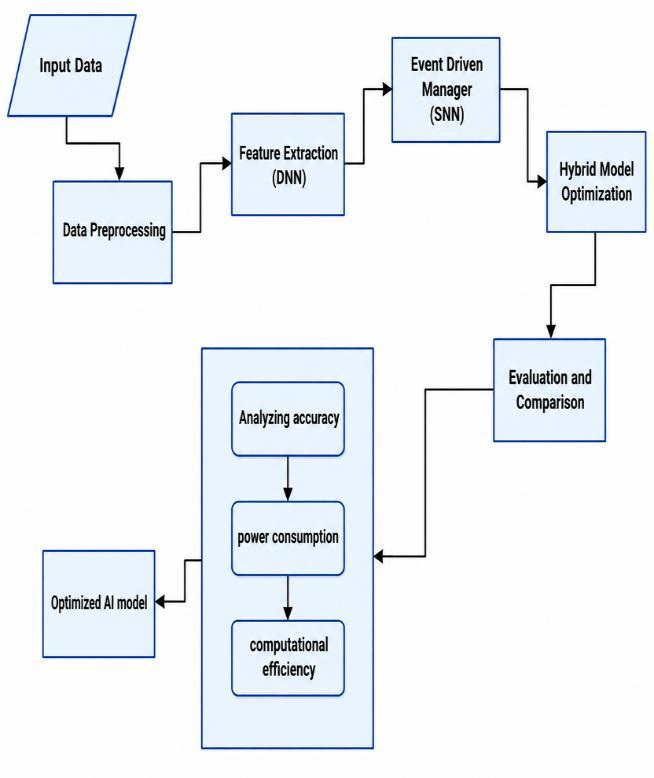
\includegraphics[width=0.72\columnwidth]{assets/images/ayan_brain_architecture.jpg}
    \captionof{figure}{Architecture of the proposed brain-inspired hybrid computing workflow.}
\end{minipage}
  \end{center}
\vspace{-0.35em}

  \subsection*{\centering\uppercase{Efficient Evaluation}}
  During evolutionary architecture search, the performance of each candidate model must be evaluated before the next generation can be produced. Training every candidate network from scratch until convergence can require many GPU-days [19]--[21]. Model evaluation consequently becomes the most time-consuming stage of the optimization process.

  \noindent
  Efficient evaluation methods reduce this cost by estimating candidate performance with less training. These approaches are commonly divided into \textbf{few-shot}, \textbf{one-shot}, and \textbf{zero-shot} evaluation. Few-shot methods train candidates for a limited number of steps, one-shot methods share parameters through a common supernetwork, and zero-shot methods use inexpensive indicators to rank architectures without full training. Such techniques make evolutionary optimization more practical for SNNs and hybrid models.

  \subsection*{\centering\uppercase{SNN Foundation}}
  In an SNN, presynaptic neurons transmit information using discrete spikes. A postsynaptic neuron integrates these incoming events and emits its own spike when the accumulated membrane potential reaches a threshold. This report adopts the widely used \textbf{Leaky Integrate-and-Fire (LIF)} neuron model [22].

  \noindent
  The membrane potential begins near a resting value \(V_{\mathrm{rest}}\). Incoming spikes increase the potential, while a leakage mechanism causes it to decay over time. When the potential reaches the firing threshold \(V_{\mathrm{th}}\), the neuron produces a spike and returns to its resting state. Because computation occurs mainly when events arrive, LIF-based systems can substantially reduce unnecessary activity.

  \begin{center}
\vspace{-0.5em}
\begin{minipage}{0.98\columnwidth}
\centering
    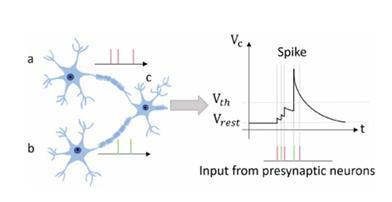
\includegraphics[width=0.75\columnwidth]{assets/images/ayan_lif_neuron.jpg}
    \captionof{figure}{Computation of an LIF neuron receiving spikes from presynaptic neurons.}
\end{minipage}
  \end{center}
\vspace{-0.35em}

  \noindent
  The architecture-search process represents an SNN using a genotype that encodes modules, neural motifs, and inter-module connections. The phenotype is the resulting executable network. Local modules are inspired by recurring neural circuits, while global cross-module connections permit information to move between distant parts of the model. This combination allows architecture evolution to explore structures beyond direct copies of conventional DNNs.

  \begin{center}
\vspace{-0.5em}
\begin{minipage}{0.98\columnwidth}
\centering
    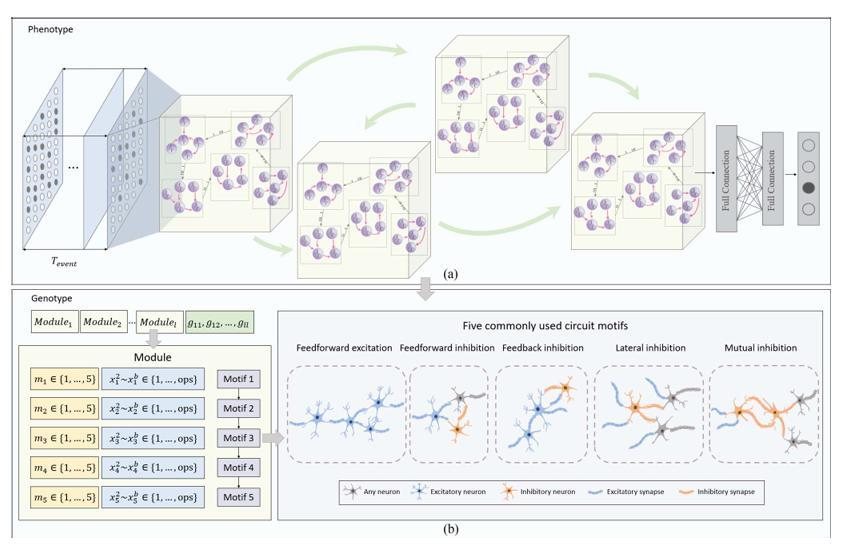
\includegraphics[width=0.85\columnwidth]{assets/images/ayan_snn_encoding.jpg}
    \captionof{figure}{Phenotype-to-genotype mapping using modular neural circuits and global connectivity.}
\end{minipage}
  \end{center}
\vspace{-0.35em}

  \subsection*{\centering\uppercase{Model Architecture and Training Protocols}}
  The hybrid model combines conventional dense processing with a spiking inference stage. Its DNN section contains three fully connected layers with 128, 64, and 32 neurons using Rectified Linear Unit (ReLU) activation. The neuromorphic section contains an SNN with 100 spiking neurons and Spike-Timing-Dependent Plasticity (STDP) learning.

  \noindent
  Input features are converted into spike trains through rate coding. Training uses the Adam optimizer with a learning rate of \(0.001\), a batch size of 32, and a maximum of 50 epochs. Early stopping limits overfitting, while data augmentation and dropout regularization with a rate of \(0.3\) improve generalization. Spike thresholds are optimized for efficient execution on the Intel Loihi framework.

  \subsection*{\centering\uppercase{Comparison with Traditional Deep Learning Architectures}}
  The hybrid system must be evaluated against an equivalent conventional deep-learning model. Accuracy indicates whether conversion to spiking computation preserves useful predictive performance. Energy savings can be expressed as the percentage reduction in power consumption, while computational cost measures processing time, operation count, latency, and memory traffic.

  {\justifying\noindent
  Traditional DNN accelerators provide high throughput for dense numerical operations, but their energy use increases with model size and repeated memory access. Neuromorphic hardware can be more efficient when inputs are sparse and event-driven. Its benefit is therefore workload-dependent: dense tasks may continue to favor GPUs or TPUs, whereas sensing, robotics, and edge applications may benefit from spike-based computation.\par}

  \subsection*{\centering\uppercase{Deep Neural Networks}}
  A Deep Neural Network is an artificial neural network containing multiple processing layers between its input and output. DNNs are constructed from neurons, weighted connections, biases, and nonlinear activation functions. Training adjusts the weights so that the network can approximate complex relationships in data [23].

  \noindent
  DNNs provide strong accuracy and mature training methods, but they generally process continuous numerical values at every layer. This produces large numbers of operations even when the input contains little new information. Their dependence on memory bandwidth and parallel arithmetic contributes to the energy cost of modern AI.

  \subsection*{\centering\uppercase{Neuromorphic Computing}}
  Neuromorphic computing uses specialized circuits and algorithms to imitate selected structural and operational principles of the brain. Memory and computation are placed close together, communication is event-driven, and SNN neurons exchange discrete spikes. These characteristics reduce data movement and allow inactive circuits to remain idle.

  \noindent
  Neuromorphic processors are particularly suitable for edge devices, where power, latency, and physical size are constrained. Hardware such as Intel Loihi, IBM TrueNorth, and SpiNNaker demonstrates the feasibility of scalable brain-inspired computation. Neuromorphic systems may also provide fault tolerance and adaptive learning, although programming tools and deployment standards remain less mature than those available for conventional deep learning.

  \begin{center}
\vspace{-0.5em}
\begin{minipage}{0.98\columnwidth}
\centering
    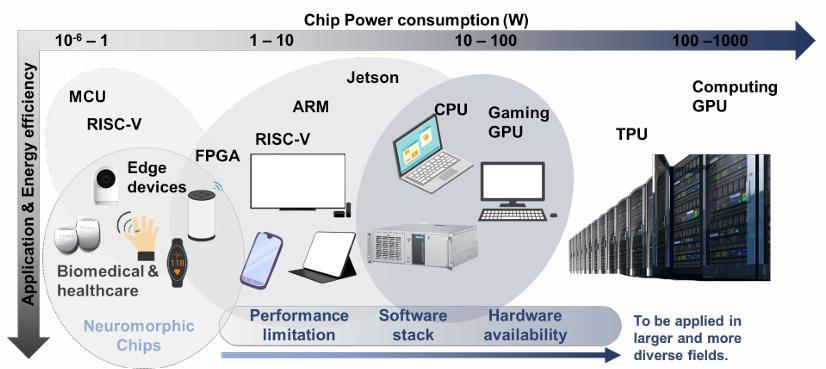
\includegraphics[width=0.85\columnwidth]{assets/images/ayan_neuromorphic_applications.jpg}
    \captionof{figure}{Neuromorphic processors occupy the low-power edge of the AI hardware landscape.}
\end{minipage}
  \end{center}
\vspace{-0.35em}

  \subsection*{\centering\uppercase{Hybrid Deep Learning and Neuromorphic Computing for Energy-Efficient AI}}
  Hybrid AI combines the high accuracy of DNNs with the energy efficiency of neuromorphic processing. Selected DNN layers can be converted into SNN stages and deployed on event-driven hardware such as Intel Loihi or SpiNNaker. The conventional portion of the model performs feature extraction, while the spiking portion handles sparse inference or temporal processing.

  \noindent
  This approach can reduce power consumption and latency for edge AI, robotics, Internet of Things devices, and always-on sensing. It also avoids the need to replace the entire deep-learning pipeline at once. However, effective conversion requires careful spike encoding, threshold optimization, accuracy preservation, and hardware-aware training.

  \begin{center}
\vspace{-0.5em}
\begin{minipage}{0.98\columnwidth}
\centering
    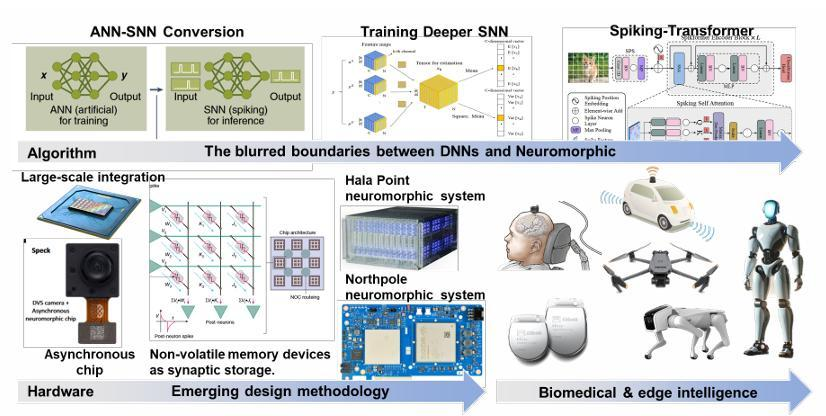
\includegraphics[width=0.85\columnwidth]{assets/images/ayan_trends.jpg}
    \captionof{figure}{Trends in neuromorphic algorithms, chips, memory technologies, and edge applications.}
\end{minipage}
  \end{center}
\vspace{-0.35em}

  \subsection*{\centering\uppercase{Conclusion and Future Scope}}
  Neuromorphic computing offers a promising approach to energy-efficient AI by replacing continuous, clock-driven processing with sparse, event-driven computation. SNNs and LIF neurons provide a foundation for brain-inspired hardware, while NAS and evolutionary optimization can discover architectures that are better suited to neuromorphic execution.

  \noindent
  Current SNN research still relies heavily on fixed structures derived from DNNs, and many NAS-based SNN models do not yet consistently outperform carefully designed conventional networks. Future work should therefore improve SNN training accuracy, develop faster evaluation strategies, and evolve architectures using modular neural motifs and long-range connections.

  \noindent
  Progress in hardware platforms such as Intel Loihi, IBM TrueNorth, and SpiNNaker can improve flexibility and computational efficiency. Hybrid models should also be tested in practical applications including healthcare diagnostics, autonomous vehicles, smart cities, industrial sensing, and robotics. Standardized frameworks for integrating DNNs with neuromorphic hardware will be essential for the large-scale adoption of energy-efficient, real-time AI systems.

  \subsection*{\centering\uppercase{References}}
  {\small
  \begingroup\justifying
  \Urlmuskip=0mu plus 1mu\relax
  \begin{enumerate}[leftmargin=*,itemsep=0.20em]
    \item J. McCarthy, M. L. Minsky, N. Rochester, et al., “A proposal for the Dartmouth summer research project on artificial intelligence, August 31, 1955,” \textit{AI Magazine}, vol. 27, no. 4, pp. 12--14, 2006.
    \item W. Q. Zhang, B. Gao, J. S. Tang, et al., “Neuro-inspired computing chips,” \textit{Nature Electronics}, vol. 3, no. 7, pp. 371--382, 2020.
    \item A. Krikelis and C. C. Weems, “Associative processing and processors,” \textit{Computer}, vol. 27, no. 11, pp. 12--17, 1994.
    \item J. Pei, L. Deng, S. Song, et al., “Towards artificial general intelligence with hybrid Tianjic chip architecture,” \textit{Nature}, vol. 572, no. 7767, pp. 106--111, 2019.
    \item W. Maass, “Networks of spiking neurons: The third generation of neural network models,” \textit{Neural Networks}, vol. 10, no. 9, pp. 1659--1671, 1997.
    \item A. Reuther, P. Michaleas, M. Jones, et al., “AI and ML accelerator survey and trends,” in \textit{Proceedings of the 2022 IEEE High Performance Extreme Computing Conference}, Waltham, MA, USA, pp. 1--10, 2022.
    \item G. I. Okolo, S. Katsigiannis, and N. Ramzan, “IEViT: An enhanced vision transformer architecture for chest X-ray image classification,” \textit{Computer Methods and Programs in Biomedicine}, vol. 226, p. 107141, Nov. 2022, doi: 10.1016/j.cmpb.2022.107141.
    \item S. Liu, J. Yu, X. Deng, and S. Wan, “FedCPF: An efficient communication federated learning approach for vehicular edge computing in 6G communication networks,” \textit{IEEE Transactions on Intelligent Transportation Systems}, vol. 23, no. 2, pp. 1616--1629, Feb. 2022, doi: 10.1109/TITS.2021.3099368.
    \item Z. Dong, X. Ji, G. Zhou, M. Gao, and D. Qi, “Multimodal neuromorphic sensory-processing system with memristor circuits for smart home applications,” \textit{IEEE Transactions on Industry Applications}, vol. 59, no. 1, pp. 47--58, Jan. 2023, doi: 10.1109/TIA.2022.3188749.
    \item “A fast and energy-efficient SNN processor with adaptive clock/event-driven computation scheme and online learning,” \textit{IEEE Xplore}. [Online]. Available: \url{https://ieeexplore.ieee.org/abstract/document/9336327}.
    \item “Edge-based collaborative training system for Artificial Intelligence of Things,” \textit{IEEE Xplore}. [Online]. Available: \url{https://ieeexplore.ieee.org/abstract/document/9699416}.
    \item T. Elsken, J. H. Metzen, and F. Hutter, “Neural architecture search: A survey,” \textit{Journal of Machine Learning Research}, vol. 20, no. 1, pp. 1997--2017, 2019.
    \item G. Ghiasi, T.-Y. Lin, and Q. V. Le, “NAS-FPN: Learning scalable feature pyramid architecture for object detection,” in \textit{Proceedings of the IEEE/CVF Conference on Computer Vision and Pattern Recognition}, pp. 7036--7045, 2019.
    \item B. Zoph and Q. V. Le, “Neural architecture search with reinforcement learning,” arXiv:1611.01578, 2016.
    \item P. Ren et al., “A comprehensive survey of neural architecture search: Challenges and solutions,” \textit{ACM Computing Surveys}, vol. 54, no. 4, pp. 1--34, 2021.
    \item K. Price, R. M. Storn, and J. A. Lampinen, \textit{Differential Evolution: A Practical Approach to Global Optimization}. New York, NY, USA: Springer-Verlag, 2006.
    \item Y. Sun, G. G. Yen, and Z. Yi, “IGD indicator-based evolutionary algorithm for many-objective optimization problems,” \textit{IEEE Transactions on Evolutionary Computation}, vol. 23, no. 2, pp. 173--187, Apr. 2019.
    \item Z. Lu et al., “NSGA-Net: Neural architecture search using multi-objective genetic algorithm,” in \textit{Proceedings of the Genetic and Evolutionary Computation Conference}, pp. 419--427, 2019.
    \item E. Real, A. Aggarwal, Y. Huang, and Q. V. Le, “Regularized evolution for image classifier architecture search,” in \textit{Proceedings of the AAAI Conference on Artificial Intelligence}, vol. 33, no. 1, pp. 4780--4789, 2019.
    \item B. Zoph and Q. V. Le, “Neural architecture search with reinforcement learning,” arXiv:1611.01578, 2016.
    \item E. Real et al., “Large-scale evolution of image classifiers,” in \textit{Proceedings of the International Conference on Machine Learning}, PMLR, pp. 2902--2911, 2017.
    \item B. Nicolas, C. Mark, and W. van Rossum, “Quantitative investigations of electrical nerve excitation treated as polarization,” \textit{Biological Cybernetics}, vol. 97, no. 5--6, p. 341, 2007.
    \item “Deep learning,” \textit{Wikipedia}. [Online]. Available: \url{https://en.wikipedia.org/wiki/Deep_learning\#Deep_neural_networks}.
  \end{enumerate}
  \par\endgroup
  }
\end{multicols}

% Exact TikZ figures imported from the author-provided LaTeX source.

\newcommand{\arjunArchitectureFigure}{%
\resizebox{0.85\columnwidth}{!}{%
    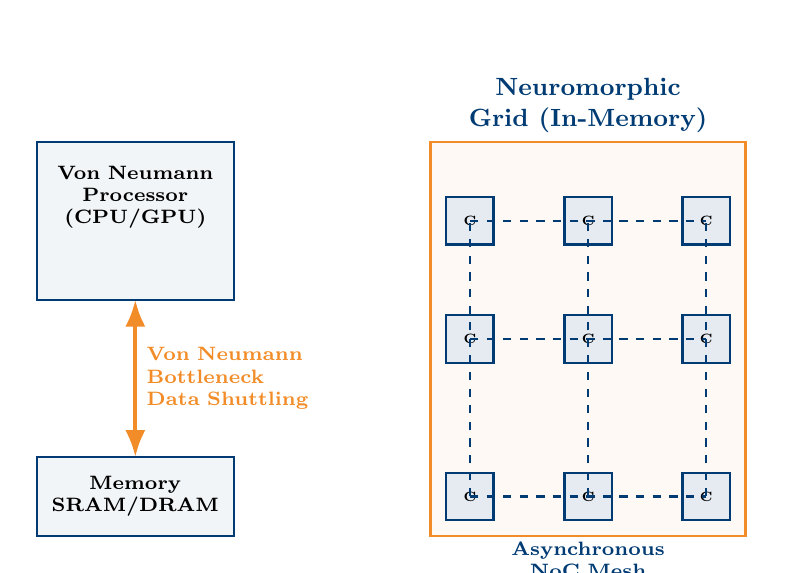
\begin{tikzpicture}[node distance=1.5cm, every node/.style={font=\scriptsize}]
        % Traditional Architecture (Von Neumann)
        \draw[thick, IEEEblue, fill=IEEEblue!5] (-3.5, 1.5) rectangle (-1.0, 3.5);
        \node[align=center, text width=2.1cm] at (-2.25, 2.8) {\textbf{Von Neumann}\\\textbf{Processor}\\\textbf{(CPU/GPU)}};
        \draw[thick, IEEEblue, fill=IEEEblue!5] (-3.5, -1.5) rectangle (-1.0, -0.5);
        \node[align=center, text width=2.5cm] at (-2.25, -1.0) {\textbf{Memory}\\\textbf{SRAM/DRAM}};
        
        \draw[<->, >=Latex, line width=1.5pt, IEEEorange] (-2.25, -0.5) -- (-2.25, 1.5) 
            node[midway, right, align=left, text width=2.2cm, text=IEEEorange] {\textbf{Von Neumann}\\\textbf{Bottleneck}\\\textbf{Data Shuttling}};

        % Neuromorphic Architecture
        \draw[thick, IEEEorange, fill=IEEEorange!5] (1.5, -1.5) rectangle (5.5, 3.5);
        \node[above, font=\small\bfseries, text=IEEEblue, text width=4.2cm, align=center] at (3.5, 3.5) {Neuromorphic Grid (In-Memory)};
        
        % Sub-grid of co-located neurocores
        \foreach \x in {2.0, 3.5, 5.0} {
            \foreach \y in {-1.0, 1.0, 2.5} {
                \draw[thick, IEEEblue, fill=IEEEblue!10] (\x-0.3, \y-0.3) rectangle (\x+0.3, \y+0.3);
                \node at (\x, \y) [scale=0.7] {\textbf{C}};
            }
        }
        % Connect the cores (NoC Router mesh)
        \draw[thick, dashed, IEEEblue] (2.0, -1.0) -- (5.0, -1.0);
        \draw[thick, dashed, IEEEblue] (2.0, 1.0) -- (5.0, 1.0);
        \draw[thick, dashed, IEEEblue] (2.0, 2.5) -- (5.0, 2.5);
        \draw[thick, dashed, IEEEblue] (2.0, -1.0) -- (2.0, 2.5);
        \draw[thick, dashed, IEEEblue] (3.5, -1.0) -- (3.5, 2.5);
        \draw[thick, dashed, IEEEblue] (5.0, -1.0) -- (5.0, 2.5);
        
        \node[align=center, text width=3.2cm, text=IEEEblue] at (3.5, -1.8) {\textbf{Asynchronous}\\\textbf{NoC Mesh}};
        
    \end{tikzpicture}%
    }%
}

\newcommand{\arjunNeuronFigure}{%
\resizebox{\columnwidth}{!}{%
    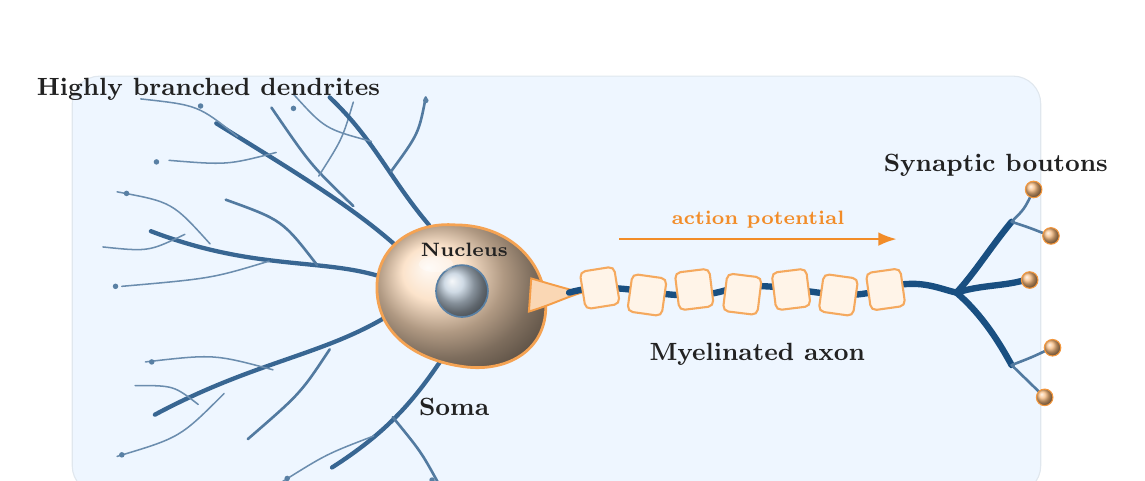
\begin{tikzpicture}[
        neuron/.style={line cap=round, line join=round},
        trunk/.style={neuron, line width=1.55pt, IEEEblue!78},
        branch/.style={neuron, line width=0.95pt, IEEEblue!68},
        twig/.style={neuron, line width=0.55pt, IEEEblue!58},
        axon/.style={neuron, line width=2.3pt, IEEEblue!90},
        label/.style={font=\small\bfseries, text=DarkGray}
    ]
        % Soft microscope-slide backdrop
        \fill[SoftBlue, rounded corners=10pt] (-4.85,-2.55) rectangle (7.45,2.75);
        \draw[IEEEblue!12, rounded corners=10pt] (-4.85,-2.55) rectangle (7.45,2.75);

        % Dense dendritic arbor around the soma: primary trunks, secondary branches, and tiny spines
        \draw[trunk] (-0.72,0.58) .. controls (-1.30,1.10) and (-2.05,1.55) .. (-3.02,2.15);
        \draw[branch] (-1.28,1.10) .. controls (-1.82,1.62) .. (-2.32,2.35);
        \draw[twig] (-1.72,1.48) .. controls (-1.42,1.95) .. (-1.28,2.42);
        \draw[twig] (-2.26,1.78) .. controls (-2.88,1.62) .. (-3.62,1.68);
        \draw[twig] (-2.75,1.98) .. controls (-3.25,2.38) .. (-3.98,2.46);

        \draw[trunk] (-0.92,0.20) .. controls (-1.68,0.44) and (-2.55,0.28) .. (-3.85,0.78);
        \draw[branch] (-1.74,0.35) .. controls (-2.18,0.92) .. (-2.90,1.18);
        \draw[twig] (-2.35,0.40) .. controls (-3.08,0.18) .. (-4.22,0.08);
        \draw[twig] (-3.10,0.62) .. controls (-3.58,1.15) .. (-4.28,1.28);
        \draw[twig] (-3.42,0.74) .. controls (-3.88,0.52) .. (-4.46,0.58);

        \draw[trunk] (-0.85,-0.30) .. controls (-1.68,-0.80) and (-2.55,-0.88) .. (-3.80,-1.55);
        \draw[branch] (-1.58,-0.72) .. controls (-1.95,-1.28) .. (-2.62,-1.86);
        \draw[twig] (-2.30,-0.98) .. controls (-3.05,-0.78) .. (-3.92,-0.88);
        \draw[twig] (-2.92,-1.28) .. controls (-3.48,-1.84) .. (-4.28,-2.08);
        \draw[twig] (-3.25,-1.42) .. controls (-3.56,-1.18) .. (-4.05,-1.18);

        \draw[trunk] (-0.32,0.86) .. controls (-0.82,1.45) and (-1.02,1.95) .. (-1.58,2.48);
        \draw[branch] (-0.80,1.54) .. controls (-0.45,2.02) .. (-0.36,2.48);
        \draw[twig] (-1.05,1.92) .. controls (-1.64,2.08) .. (-2.04,2.52);

        \draw[trunk] (-0.18,-0.88) .. controls (-0.52,-1.38) and (-0.86,-1.78) .. (-1.55,-2.22);
        \draw[branch] (-0.78,-1.58) .. controls (-0.42,-2.02) .. (-0.20,-2.42);
        \draw[twig] (-1.02,-1.82) .. controls (-1.62,-2.05) .. (-2.18,-2.40);

        % Small dendritic spines for a more biological silhouette
        \foreach \x/\y in {-3.78/1.66,-3.22/2.37,-2.04/2.34,-4.16/1.26,-4.30/0.08,-3.84/-0.88,-4.22/-2.06,-2.12/-2.36,-0.28/-2.38,-0.36/2.44} {
            \fill[IEEEblue!65] (\x,\y) circle (0.035);
        }

        % Irregular soma and nucleus with a more cell-like outline
        \shade[ball color=IEEEorange!32, draw=IEEEorange!80, line width=1pt]
            (0.02,0.86)
            .. controls (0.62,0.86) and (1.10,0.48) .. (1.16,-0.08)
            .. controls (1.22,-0.72) and (0.68,-1.02) .. (0.12,-0.94)
            .. controls (-0.48,-0.86) and (-1.00,-0.52) .. (-0.98,0.10)
            .. controls (-0.96,0.62) and (-0.48,0.90) .. (0.02,0.86) -- cycle;
        \shade[ball color=IEEEblue!25, draw=IEEEblue!65, line width=0.6pt] (0.10,0.02) circle (0.33);
        \fill[white!45, opacity=0.35] (-0.23,0.36) ellipse (0.22 and 0.10);

        % Axon hillock and longer axon with myelin gaps (nodes of Ranvier)
        \filldraw[fill=IEEEorange!35, draw=IEEEorange!85, line width=0.7pt]
            (0.98,0.18) .. controls (1.25,0.10) and (1.46,0.04) .. (1.62,0.00)
            .. controls (1.42,-0.06) and (1.22,-0.16) .. (0.95,-0.24) -- cycle;
        \draw[axon] (1.46,0.00) .. controls (2.15,0.20) and (2.75,-0.18) .. (3.45,0.03)
                         .. controls (4.10,0.22) and (4.82,-0.18) .. (5.42,0.04)
                         .. controls (5.88,0.20) and (6.15,0.05) .. (6.38,0.00);
        \foreach \x/\y/\rot in {1.85/0.06/9,2.45/-0.03/-8,3.05/0.04/7,3.66/-0.02/-7,4.28/0.04/7,4.88/-0.03/-8,5.48/0.04/8} {
            \begin{scope}[shift={(\x,\y)}, rotate=\rot]
                \filldraw[fill=SoftOrange, draw=IEEEorange!75, line width=0.75pt, rounded corners=2pt]
                    (-0.22,-0.24) rectangle (0.22,0.24);
            \end{scope}
        }

        % Rich axon terminal arbor with bouton-like endpoints
        \draw[axon] (6.38,0.00) .. controls (6.62,0.26) and (6.80,0.56) .. (7.08,0.90);
        \draw[axon] (6.38,0.00) .. controls (6.70,0.10) and (6.98,0.08) .. (7.25,0.16);
        \draw[axon] (6.38,0.00) .. controls (6.66,-0.24) and (6.88,-0.55) .. (7.08,-0.92);
        \draw[branch] (7.08,0.90) .. controls (7.24,1.06) .. (7.34,1.26);
        \draw[branch] (7.08,0.90) .. controls (7.32,0.82) .. (7.52,0.74);
        \draw[branch] (7.08,-0.92) .. controls (7.26,-1.10) .. (7.45,-1.28);
        \draw[branch] (7.08,-0.92) .. controls (7.34,-0.82) .. (7.55,-0.72);
        \foreach \p in {(7.36,1.31),(7.58,0.72),(7.31,0.16),(7.50,-1.33),(7.60,-0.70)} {
            \shade[ball color=IEEEorange!60, draw=IEEEorange!90] \p circle (0.105);
        }

        % Direction of spike propagation
        \draw[-Latex, thick, IEEEorange] (2.10,0.68) -- node[above, font=\scriptsize\bfseries, text=IEEEorange] {action potential} (5.62,0.68);

        % Labels
        \node[label] at (-3.12,2.58) {Highly branched dendrites};
        \node[label] at (0,-1.45) {Soma};
        \node[label] at (0.13,0.55) {\scriptsize Nucleus};
        \node[label] at (3.85,-0.78) {Myelinated axon};
        \node[label] at (6.88,1.62) {Synaptic boutons};
    \end{tikzpicture}%
    }%
}

\newcommand{\arjunLIFFigure}{%
\resizebox{\columnwidth}{!}{%
    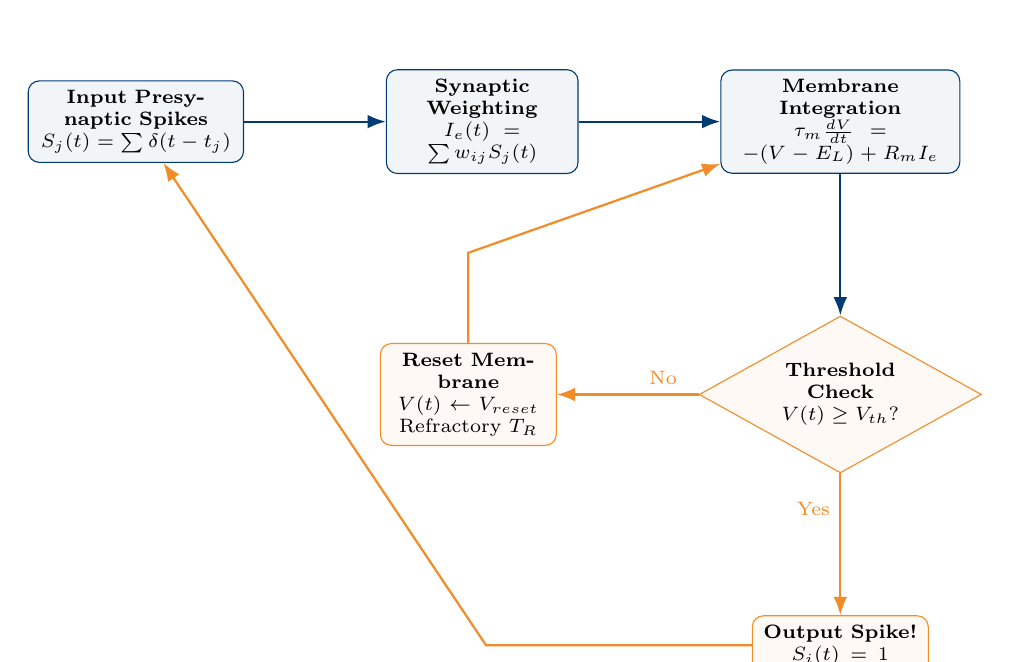
\begin{tikzpicture}[node distance=1.8cm, auto, >=Latex, every node/.style={font=\scriptsize}]
        % Flowchart nodes
        \node [draw=IEEEblue, fill=IEEEblue!5, rectangle, rounded corners, align=center, text width=2.5cm] (input) {\textbf{Input Presynaptic Spikes}\\$S_j(t) = \sum \delta(t-t_j)$};
        \node [draw=IEEEblue, fill=IEEEblue!5, rectangle, rounded corners, align=center, text width=2.2cm, right=of input] (synapse) {\textbf{Synaptic Weighting}\\$I_e(t) = \sum w_{ij} S_j(t)$};
        \node [draw=IEEEblue, fill=IEEEblue!5, rectangle, rounded corners, align=center, text width=2.8cm, right=of synapse] (integrate) {\textbf{Membrane Integration}\\$\tau_m \frac{dV}{dt} = -(V - E_L) + R_m I_e$};
        \node [draw=IEEEorange, fill=IEEEorange!5, diamond, align=center, aspect=1.8, text width=1.5cm, below=of integrate] (threshold) {\textbf{Threshold Check}\\$V(t) \ge V_{th}$?};
        \node [draw=IEEEorange, fill=IEEEorange!5, rectangle, rounded corners, align=center, text width=2.0cm, left=of threshold] (reset) {\textbf{Reset Membrane}\\$V(t) \leftarrow V_{reset}$\\Refractory $T_R$};
        \node [draw=IEEEorange, fill=IEEEorange!5, rectangle, rounded corners, align=center, text width=2.0cm, below=of threshold] (fire) {\textbf{Output Spike!}\\$S_i(t) = 1$};

        % Paths
        \path [draw, ->, thick, IEEEblue] (input) -- (synapse);
        \path [draw, ->, thick, IEEEblue] (synapse) -- (integrate);
        \path [draw, ->, thick, IEEEblue] (integrate) -- (threshold);
        \path [draw, ->, thick, IEEEorange] (threshold) -- node [near start, left] {Yes} (fire);
        \path [draw, ->, thick, IEEEorange] (threshold) -- node [near start, above] {No} (reset);
        \path [draw, ->, thick, IEEEorange] (reset) -- ++(0, 1.8) -- (integrate);
        \path [draw, ->, thick, IEEEorange] (fire) -- ++(-4.5, 0) -- (input);
    \end{tikzpicture}%
    }%
}

\newcommand{\arjunMemristorFigure}{%
\resizebox{\columnwidth}{!}{%
    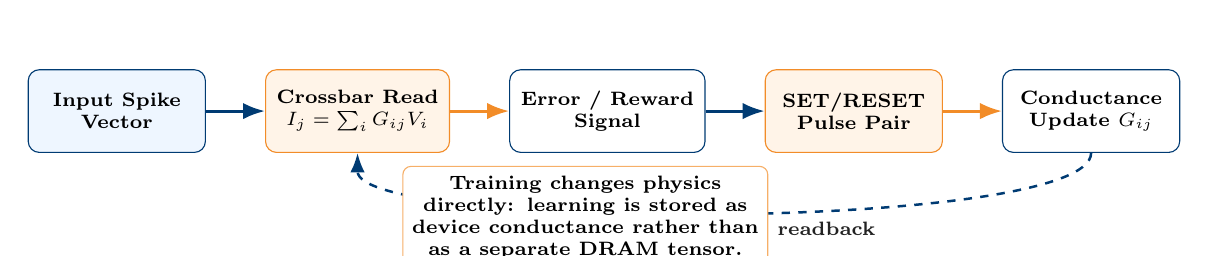
\begin{tikzpicture}[node distance=0.75cm,>=Latex,every node/.style={font=\scriptsize\bfseries, align=center}, flowstep/.style={draw, rounded corners=4pt, minimum width=2.25cm, minimum height=1.05cm, inner sep=4pt}]
        \node[flowstep, draw=IEEEblue, fill=SoftBlue] (input) {Input Spike\\Vector};
        \node[flowstep, draw=IEEEorange, fill=SoftOrange, right=of input] (read) {Crossbar Read\\$I_j=\sum_iG_{ij}V_i$};
        \node[flowstep, draw=IEEEblue, fill=white, right=of read] (error) {Error / Reward\\Signal};
        \node[flowstep, draw=IEEEorange, fill=SoftOrange, right=of error] (pulse) {SET/RESET\\Pulse Pair};
        \node[flowstep, draw=IEEEblue, fill=white, right=of pulse] (conductance) {Conductance\\Update $G_{ij}$};
        \draw[-Latex, line width=1.1pt, IEEEblue] (input) -- (read);
        \draw[-Latex, line width=1.1pt, IEEEorange] (read) -- (error);
        \draw[-Latex, line width=1.1pt, IEEEblue] (error) -- (pulse);
        \draw[-Latex, line width=1.1pt, IEEEorange] (pulse) -- (conductance);
        \draw[-Latex, dashed, line width=0.9pt, IEEEblue] (conductance.south) .. controls +(0,-1.0) and +(0,-1.0) .. node[below, text=DarkGray] {verify-and-correct readback} (read.south);
        \node[draw=IEEEorange!70, fill=white, rounded corners=3pt, text width=4.4cm] at (5.95,-1.35) {Training changes physics directly: learning is stored as device conductance rather than as a separate DRAM tensor.};
    \end{tikzpicture}%
    }%
}

\newcommand{\arjunEdgeFigure}{%
\resizebox{\columnwidth}{!}{%
    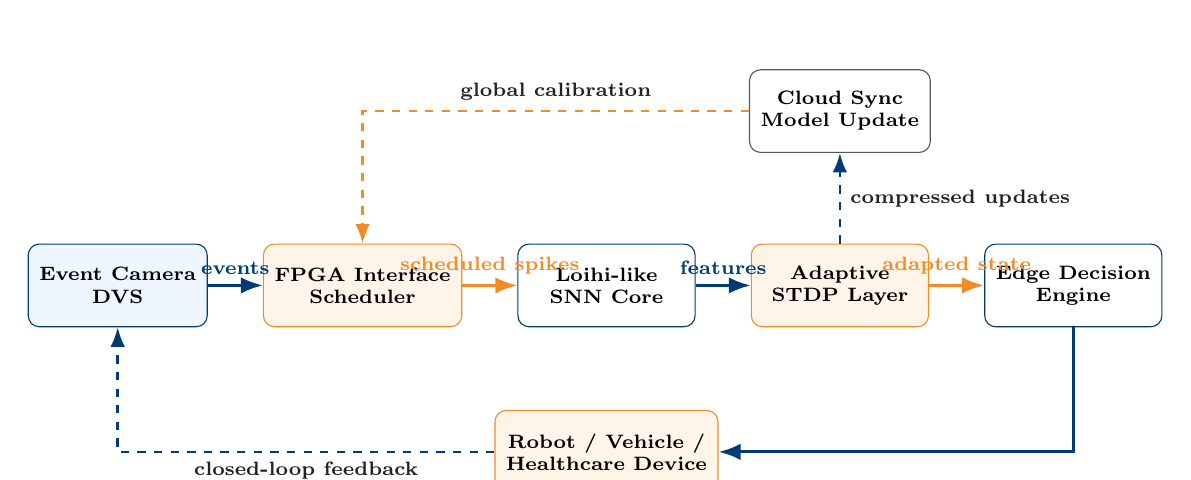
\begin{tikzpicture}[node distance=0.7cm,>=Latex,every node/.style={font=\scriptsize\bfseries, align=center}, edgeblock/.style={draw, rounded corners=4pt, minimum width=2.25cm, minimum height=1.05cm, inner sep=4pt}]
        \node[edgeblock, draw=IEEEblue, fill=SoftBlue] (dvs) {Event Camera\\DVS};
        \node[edgeblock, draw=IEEEorange, fill=SoftOrange, right=of dvs] (fpga) {FPGA Interface\\Scheduler};
        \node[edgeblock, draw=IEEEblue, fill=white, right=of fpga] (snn) {Loihi-like\\SNN Core};
        \node[edgeblock, draw=IEEEorange, fill=SoftOrange, right=of snn] (stdp) {Adaptive\\STDP Layer};
        \node[edgeblock, draw=IEEEblue, fill=white, right=of stdp] (decision) {Edge Decision\\Engine};
        \node[edgeblock, draw=DarkGray!75, fill=white, above=1.15cm of stdp] (cloud) {Cloud Sync\\Model Update};
        \node[edgeblock, draw=IEEEorange, fill=SoftOrange, below=1.05cm of snn] (actuator) {Robot / Vehicle /\\Healthcare Device};

        \draw[-Latex, line width=1.1pt, IEEEblue] (dvs) -- node[above] {events} (fpga);
        \draw[-Latex, line width=1.1pt, IEEEorange] (fpga) -- node[above] {scheduled spikes} (snn);
        \draw[-Latex, line width=1.1pt, IEEEblue] (snn) -- node[above] {features} (stdp);
        \draw[-Latex, line width=1.1pt, IEEEorange] (stdp) -- node[above] {adapted state} (decision);
        \draw[-Latex, line width=1.1pt, IEEEblue] (decision.south) |- (actuator.east);
        \draw[-Latex, dashed, line width=0.9pt, IEEEblue] (stdp) -- node[right, text=DarkGray] {compressed updates} (cloud);
        \draw[-Latex, dashed, line width=0.9pt, IEEEorange] (cloud.west) -| node[pos=0.25, above, text=DarkGray] {global calibration} (fpga.north);
        \draw[-Latex, dashed, line width=0.9pt, IEEEblue] (actuator.west) -| node[pos=0.25, below, text=DarkGray] {closed-loop feedback} (dvs.south);
    \end{tikzpicture}%
    }%
}

\newcommand{\arjunHybridFigure}{%
\resizebox{\columnwidth}{!}{%
    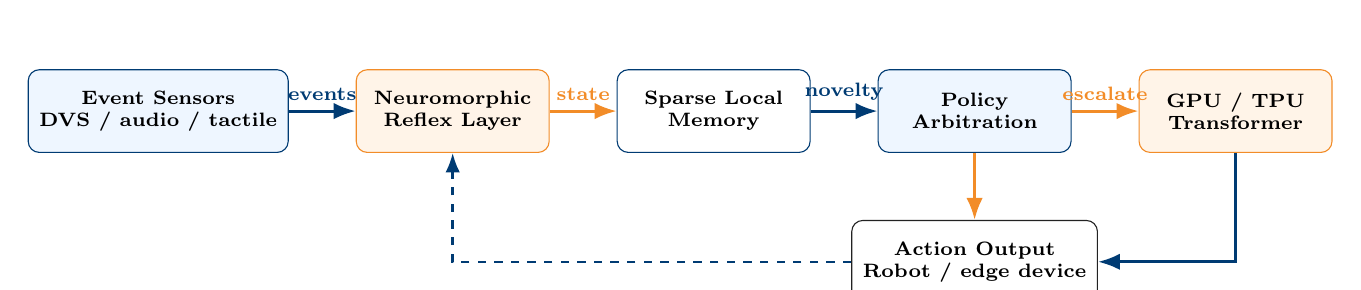
\begin{tikzpicture}[node distance=0.85cm, every node/.style={font=\scriptsize\bfseries, align=center}, block/.style={draw, rounded corners=4pt, minimum width=2.45cm, minimum height=1.05cm, inner sep=4pt}]
        \node[block, fill=SoftBlue, draw=IEEEblue] (sensor) {Event Sensors\\DVS / audio / tactile};
        \node[block, fill=SoftOrange, draw=IEEEorange, right=of sensor] (snn) {Neuromorphic\\Reflex Layer};
        \node[block, fill=white, draw=IEEEblue, right=of snn] (memory) {Sparse Local\\Memory};
        \node[block, fill=SoftBlue, draw=IEEEblue, right=of memory] (arbiter) {Policy\\Arbitration};
        \node[block, fill=SoftOrange, draw=IEEEorange, right=of arbiter] (gpu) {GPU / TPU\\Transformer};
        \node[block, fill=white, draw=DarkGray, below=of arbiter] (robot) {Action Output\\Robot / edge device};

        \draw[-Latex, line width=1.1pt, IEEEblue] (sensor) -- node[above] {events} (snn);
        \draw[-Latex, line width=1.1pt, IEEEorange] (snn) -- node[above] {state} (memory);
        \draw[-Latex, line width=1.1pt, IEEEblue] (memory) -- node[above] {novelty} (arbiter);
        \draw[-Latex, line width=1.1pt, IEEEorange] (arbiter) -- node[above] {escalate} (gpu);
        \draw[-Latex, line width=1.1pt, IEEEblue] (gpu.south) |- (robot.east);
        \draw[-Latex, line width=1.1pt, IEEEorange] (arbiter) -- (robot);
        \draw[-Latex, dashed, line width=0.9pt, IEEEblue] (robot.west) -| (snn.south);
    \end{tikzpicture}%
    }%
}

\begin{center}
  \section{\capitalisewords{Brain-Inspired Neuromorphic Computing Chips for Energy-Efficient Artificial Intelligence}}
  Arjun Mitra, 3$^{rd}$ Year, ECE
\end{center}

\setcounter{figure}{0}
\setcounter{table}{0}

\begin{multicols}{2}
  \begin{abstract}
    \bfseries
    The rapid growth of artificial intelligence has exposed a fundamental limitation of conventional computing: moving data repeatedly between processors and memory consumes more energy than many arithmetic operations themselves. Neuromorphic computing addresses this limitation by reproducing selected principles of the nervous system in hardware, including event-driven communication, distributed memory, massively parallel processing, and adaptive synaptic connections. Instead of continuously executing clocked instructions, neuromorphic chips communicate through sparse electrical spikes and activate computation only when relevant events occur.
    This report examines the biological foundations, mathematical models, learning rules, semiconductor architectures, and emerging materials that enable neuromorphic systems. Representative platforms such as IBM TrueNorth, Intel Loihi and Loihi~2, SpiNNaker, and Intel Hala Point are compared with conventional accelerators. The report also evaluates memristive crossbars, event-based sensing, edge robotics, photonic and quantum approaches, and the environmental implications of brain-inspired hardware. Finally, a hybrid architecture is proposed in which neuromorphic processors perform continuous low-power perception while conventional GPU or TPU accelerators are invoked selectively for dense reasoning. The analysis shows that neuromorphic chips are unlikely to replace all conventional processors, but they can become an important energy-efficient companion technology for sparse, time-dependent, and always-on intelligence.

    \vspace{2em}
    {\justifying\noindent\textbf{Keywords:} Neuromorphic Computing, Spiking Neural Networks, Loihi, TrueNorth, Hala Point, Memristor, Event-Driven AI, STDP, Edge Intelligence, Green AI.\par}
  \end{abstract}
  \vspace{-0.6em}
  \subsection*{\centering\uppercase{Introduction}}
  Modern AI systems achieve remarkable performance by executing enormous numbers of multiply--accumulate operations on GPUs and other dense accelerators. Their success, however, comes with high energy consumption, substantial memory traffic, and increasingly expensive cooling infrastructure. In a conventional von Neumann computer, memory and processing are physically separated. Weights and activations must therefore travel repeatedly through a limited communication path, producing the well-known von Neumann bottleneck.

  \noindent
  The human brain demonstrates a different computational strategy. Approximately 86 billion neurons operate through local, asynchronous interactions while the complete organ consumes only about 20~W. Biological intelligence is not obtained by forcing every neuron to update at every instant. Neurons remain mostly inactive and communicate only when their membrane potential crosses a threshold. Memory and computation are also closely linked because information is stored in the strengths of synaptic connections.

  \noindent
  Neuromorphic engineering, introduced as a formal hardware discipline by Carver Mead, translates these principles into electronic circuits. Its goal is not to reproduce the brain in every biological detail, but to identify useful computational properties---sparsity, local state, temporal coding, parallelism, and adaptation---and implement them efficiently in silicon.

  \begin{center}
\vspace{-0.5em}
\begin{minipage}{0.98\columnwidth}
\centering
    \arjunArchitectureFigure
    \captionof{figure}{Architectural shift from processor--memory data shuttling to an asynchronous neuromorphic grid with local memory and computation.}
\end{minipage}
  \end{center}
\vspace{-0.35em}

  \subsection*{\centering\uppercase{From Biological Neurons to Electronic Circuits}}
  A biological neuron receives signals through dendrites, integrates them in the soma, and transmits an action potential along the axon when sufficient excitation is accumulated. Synapses determine the influence of one neuron on another, and their strengths change with experience. This provides a natural model for computation in which both information and time are significant.

  \begin{center}
\vspace{-0.5em}
\begin{minipage}{0.98\columnwidth}
\centering
    \arjunNeuronFigure
    \captionof{figure}{Biological neuron structure that inspires artificial dendrites, soma integration, axonal communication, and programmable synaptic weights.}
\end{minipage}
  \end{center}

  In digital neuromorphic hardware, each neuron is represented by a small state machine or circuit. Incoming spikes update its internal voltage, leakage reduces that voltage with time, and an output spike is generated at a threshold. Communication commonly uses Address-Event Representation (AER), in which a transmitted packet identifies the firing neuron rather than carrying a continuous-valued activation.

  Table~1 compares conventional and neuromorphic computing principles.
  \begin{center}
\vspace{-0.5em}
\begin{minipage}{0.98\columnwidth}
\centering
    \scriptsize
    \captionof{table}{Conventional and neuromorphic computing principles}
    \setlength{\tabcolsep}{3pt}
    \renewcommand{\arraystretch}{1.25}
    \begin{tabular}{@{}>{\RaggedRight\arraybackslash}p{0.25\columnwidth}
      >{\RaggedRight\arraybackslash}p{0.31\columnwidth}
      >{\RaggedRight\arraybackslash}p{0.34\columnwidth}@{}}
      \toprule
      \textbf{Feature} & \textbf{Von Neumann} & \textbf{Neuromorphic} \\
      \midrule
      Processing & Sequential or batched & Massively parallel \\
      Memory & Separate hierarchy & Distributed near compute \\
      Timing & Global clock & Event-driven, asynchronous \\
      Data & Dense numeric words & Sparse spike events \\
      Learning & Usually off-chip & Local or on-chip possible \\
      Idle power & Continual activity & Units sleep between events \\
      \bottomrule
    \end{tabular}
\end{minipage}
  \end{center}
\vspace{-0.35em}

  \subsection*{\centering\uppercase{Spiking Neural Network Fundamentals}}
  Spiking Neural Networks (SNNs) are often described as the third generation of neural networks because they represent both the occurrence and timing of neural activity. The spike train emitted by neuron $i$ can be written as
  \[
    S_i(t)=\sum_f \delta\!\left(t-t_i^{(f)}\right),
  \]
  where $t_i^{(f)}$ is the time of its $f$th spike. Information may be represented by the average firing rate, the exact timing of individual spikes, the order of spikes, or the synchrony of a population.

  \subsubsection*{Leaky Integrate-and-Fire Model}
  The Leaky Integrate-and-Fire (LIF) neuron provides a practical balance between biological meaning and hardware simplicity. Its membrane voltage is commonly modelled by
  \[
    \tau_m\frac{dV}{dt}=-(V-E_L)+R_m I_e(t),
  \]
  where $\tau_m$ is the membrane time constant, $E_L$ is the resting potential, $R_m$ is the membrane resistance, and $I_e(t)$ is the input current. When $V$ reaches a threshold $V_{th}$, the neuron emits a spike, resets, and may enter a short refractory period.

  \begin{center}
\vspace{-0.5em}
\begin{minipage}{0.98\columnwidth}
\centering
    \arjunLIFFigure
    \captionof{figure}{Operational flow of a LIF neuron from presynaptic spikes and weighted integration to threshold firing and reset.}
\end{minipage}
  \end{center}

  Rate coding is robust and easy to decode but may require many spikes and longer observation windows. Temporal coding can transmit information with fewer events and lower latency, but it is more sensitive to timing noise. Practical systems often combine both approaches depending on the sensor, task, and available hardware.

  \subsection*{\centering\uppercase{Learning and Synaptic Plasticity}}
  Biological learning occurs largely through changes in synaptic strength. A widely used local rule is Spike-Timing-Dependent Plasticity (STDP), which adjusts a synapse according to the interval $\Delta t=t_{post}-t_{pre}$ between pre- and postsynaptic spikes:
  \[
    \Delta w=
    \begin{cases}
      A_+e^{-\Delta t/\tau_+}, & \Delta t>0,\\
      -A_-e^{\Delta t/\tau_-}, & \Delta t<0.
    \end{cases}
  \]
  A presynaptic spike arriving shortly before a postsynaptic spike strengthens the connection, while the reverse order weakens it. Because only local timing information is required, STDP is attractive for on-chip and continual learning.

  \noindent
  Deep SNNs are also trained using surrogate gradients. During the forward pass, neurons retain their discrete threshold behaviour. During backpropagation, the zero or undefined derivative of the spike function is replaced by a smooth approximation. This makes conventional gradient-based optimisation possible while retaining sparse event-driven inference. Other approaches include conversion of trained Artificial Neural Networks (ANNs) into SNNs and local error rules such as the Prescribed Error Sensitivity method.

  \subsection*{\centering\uppercase{Neuromorphic Chip Architectures}}
  A neuromorphic processor contains many small cores connected by a packet-routing network. Each core stores neuron states and synaptic weights locally, processes incoming spike events, and forwards new events only when neurons fire. This reduces long-distance memory transfers and allows inactive regions to consume little dynamic power.

  Table~2 lists representative neuromorphic platforms.
  \begin{center}
\vspace{-0.5em}
\begin{minipage}{0.98\columnwidth}
\centering
    \scriptsize
    \captionof{table}{Representative neuromorphic platforms}
    \setlength{\tabcolsep}{2.5pt}
    \renewcommand{\arraystretch}{1.2}
    \begin{tabular}{@{}>{\RaggedRight\arraybackslash}p{0.20\columnwidth}
      >{\RaggedRight\arraybackslash}p{0.19\columnwidth}
      >{\RaggedRight\arraybackslash}p{0.23\columnwidth}
      >{\RaggedRight\arraybackslash}p{0.29\columnwidth}@{}}
      \toprule
      \textbf{Platform} & \textbf{Scale} & \textbf{Learning} & \textbf{Distinctive feature} \\
      \midrule
      IBM TrueNorth & 1M neurons & Offline & 4,096 low-power cores \\
      Intel Loihi & 131k neurons & On-chip & Programmable plasticity \\
      Loihi 2 & Up to 1M/chip & On-chip & Graded events and improved cores \\
      SpiNNaker & Many ARM cores & Software-defined & Real-time large SNN simulation \\
      Hala Point & 1.15B neurons & Distributed & 1,152 Loihi 2 chips \\
      \bottomrule
    \end{tabular}
\end{minipage}
  \end{center}
\vspace{-0.35em}

  \subsubsection*{IBM TrueNorth}
  TrueNorth demonstrated that one million programmable spiking neurons and 256 million synapses could be integrated into a low-power many-core device. Its 4,096 cores communicate through a scalable event-routing network. The architecture is efficient for inference but does not provide the flexible on-chip learning available in later systems.

  \subsubsection*{Intel Loihi and Loihi 2}
  Intel Loihi introduced programmable learning engines within each neuromorphic core, enabling local plasticity and adaptation without constant host intervention. Loihi~2 increased neuron capacity, event flexibility, connectivity, and processing speed while supporting Intel's Lava software framework. Hala Point scales 1,152 Loihi~2 chips to approximately 1.15 billion neurons and 128 billion synapses, showing that neuromorphic systems can reach brain-scale neuron counts in research hardware.

  \subsubsection*{SpiNNaker}
  SpiNNaker uses large numbers of conventional ARM processor cores linked by a specialised multicast network. It sacrifices some custom-circuit efficiency in exchange for flexibility, making it valuable for real-time neuroscience simulation and experiments with large, heterogeneous spiking networks.

  \subsection*{\centering\uppercase{Memristive Synapses and In-Memory Computing}}
  A memristor is a non-volatile device whose conductance depends on its electrical history. Conductance can represent a synaptic weight, making memristors attractive for dense, persistent, and analog synapse arrays. In a crossbar, input voltages are applied along rows and column currents naturally perform matrix--vector multiplication:
  \[
    I_j=\sum_i G_{ij}V_i,
  \]
  where $G_{ij}$ is the programmed conductance at cross-point $(i,j)$. The computation occurs where the weights are stored, greatly reducing data movement.

  \begin{center}
\vspace{-0.5em}
\begin{minipage}{0.98\columnwidth}
\centering
    \arjunMemristorFigure
    \captionof{figure}{Memristive training loop using crossbar readout, an error or reward signal, programming pulses, and conductance updates.}
\end{minipage}
  \end{center}

  {\justifying
  Candidate technologies include Resistive RAM, phase-change memory, and hafnium-oxide devices. Important obstacles remain: device-to-device variation, limited endurance, nonlinear programming, conductance drift, peripheral converter overhead, and the difficulty of obtaining precise symmetric weight updates. Hybrid analog--digital control is therefore likely to remain necessary.\par}

  \subsection*{\centering\uppercase{Edge Intelligence, Sensors, and Robotics}}
  Neuromorphic processors are particularly suitable for edge systems that must observe the environment continuously while operating from a small battery. Dynamic Vision Sensors report changes in brightness rather than sending complete image frames. Their output is naturally sparse, asynchronous, and compatible with SNNs. Similar principles apply to event-based microphones, tactile arrays, biomedical signals, and industrial anomaly sensors.

  \noindent
  In robotics, low-latency spike processing can support obstacle avoidance, motor control, localisation, gesture recognition, and sensor fusion. The greatest advantage appears when the complete pipeline is event-driven. Converting conventional frames into spikes or repeatedly moving data back to a host processor can eliminate much of the energy benefit.

  \subsection*{\centering\uppercase{Proposed Hybrid Neuromorphic Edge Architecture}}
  A practical deployment model combines specialised components rather than forcing every task onto one processor. The proposed architecture begins with event cameras or other sparse sensors. An FPGA interface schedules and filters events, a Loihi-like SNN core extracts temporal features, and an adaptive STDP layer updates selected local representations. An edge decision engine then controls a robot, vehicle, or healthcare device. Only compressed model updates and anomaly summaries are synchronised with the cloud.

  \begin{center}
\vspace{-0.5em}
\begin{minipage}{0.98\columnwidth}
\centering
    \arjunEdgeFigure
    \captionof{figure}{Proposed closed-loop edge architecture combining event sensing, FPGA scheduling, SNN inference, local adaptation, decisions, and selective cloud synchronisation.}
\end{minipage}
  \end{center}

  This design reduces bandwidth, improves response time, and keeps sensitive raw data near its source. It also separates fast local decisions from slower global calibration. Safety-critical systems should retain deterministic fallback logic, confidence thresholds, and conventional verification pathways.

  \subsection*{\centering\uppercase{Photonics, Quantum Devices, and Emerging Directions}}
  Photonic neuromorphic processors use light for communication and computation. Optical interference and wavelength multiplexing can provide high bandwidth and parallel matrix operations with low propagation delay. Phase-change photonic memories can retain analog weights without continuous power. The main challenges are optical loss, fabrication variability, device size, electro-optic conversion, and integration with electronic control.

  \noindent
  Quantum neuromorphic computing is more speculative. It investigates whether quantum states, stochastic sampling, and quantum sensing can be combined with neural dynamics. Near-term impact is more likely to come from quantum-inspired algorithms and specialised sensors than from a universal quantum replacement for neuromorphic chips.

  \subsection*{\centering\uppercase{Sustainability and Green AI}}
  Neuromorphic hardware can reduce operational energy when workloads are sparse. If only a fraction $\alpha$ of neurons is active and only a fraction $\gamma$ of connections is used, the effective computation may be approximated as
  \[
    C_{active}\approx\alpha\gamma C_{dense}.
  \]
  Very small values of $\alpha$ and $\gamma$ explain why event-driven hardware can outperform dense accelerators on suitable sensory and optimisation tasks.

  \noindent
  Energy claims must nevertheless be evaluated at system level. Sensor conversion, host processors, data movement, cooling, training, fabrication, and embodied carbon can dominate the chip-level savings. Fair comparisons should report accuracy, latency, total energy per decision, hardware utilisation, and the complete measurement boundary rather than isolated operations per watt.

  \subsection*{\centering\uppercase{Critical Analysis and Research Gaps}}
  Despite impressive prototypes, several barriers prevent widespread adoption:
  \begin{itemize}\justifying
    \item \textbf{Software fragmentation:} platforms use different neuron models, compilers, learning rules, and programming interfaces.
    \item \textbf{Training difficulty:} temporal credit assignment remains more difficult than training conventional dense networks.
    \item \textbf{Benchmark inconsistency:} energy and accuracy are often reported under different assumptions, making comparisons unreliable.
    \item \textbf{Workload mismatch:} transformer models and other dense workloads do not automatically benefit from spike-based execution.
    \item \textbf{Device variability:} analog memories require calibration and error-tolerant algorithms.
    \item \textbf{Commercial integration:} developers need stable toolchains, standard interfaces, debugging tools, and cost-effective packaging.
  \end{itemize}

  Neuromorphic attention mechanisms may reduce transformer cost by activating only important tokens, channels, or time steps. If conventional scaled dot-product attention is
  \[
    \operatorname{Attention}(Q,K,V)=
    \operatorname{softmax}\!\left(\frac{QK^{T}}{\sqrt{d_k}}\right)V,
  \]
  a spike-gated implementation can avoid portions of the computation when the corresponding queries or keys are inactive. This is promising, but current large-language-model workloads still favour dense GPU and TPU hardware.

  \begin{center}
\vspace{-0.5em}
\begin{minipage}{0.98\columnwidth}
\centering
    \arjunHybridFigure
    \captionof{figure}{Hybrid computing proposal: neuromorphic hardware handles continuous sparse perception, while a GPU or TPU is activated for semantic reasoning and planning.}
\end{minipage}
  \end{center}

  The most realistic near-term system is therefore heterogeneous. Neuromorphic cores can manage always-on perception, anomaly detection, reflex control, and adaptive filtering. Conventional accelerators can handle large dense models, global optimisation, and high-level planning. The design principle is simple: spikes handle time-sensitive sparse activity; GPUs handle abstraction-intensive dense computation.

  \subsection*{\centering\uppercase{Conclusion}}
  Neuromorphic computing provides a credible hardware response to the energy and data-movement limitations of conventional AI. By co-locating memory and processing, communicating through sparse events, and supporting local adaptation, neuromorphic chips can deliver very low latency and energy consumption on workloads that contain temporal structure and limited activity.

  \noindent
  TrueNorth established the feasibility of million-neuron digital hardware, Loihi added programmable on-chip learning, SpiNNaker demonstrated flexible large-scale real-time simulation, and Hala Point extended Loihi~2 to more than a billion neurons. Memristive and photonic technologies may improve density and efficiency further, although manufacturing variability and peripheral circuitry remain substantial challenges.

  \noindent
  Neuromorphic systems should not be judged as universal replacements for CPUs, GPUs, or TPUs. Their strongest role is as specialised accelerators within heterogeneous systems, particularly for event-based sensing, edge robotics, biomedical monitoring, and other always-on applications. Progress in common software tools, reproducible benchmarks, reliable devices, and hybrid architectures will determine whether brain-inspired computing moves from research platforms to routine engineering practice.

  \subsection*{\centering\uppercase{References}}
  \footnotesize
  \begin{enumerate}
    \item C. D. Schuman et al., “A Survey of Neuromorphic Computing and Neural Networks in Hardware,” arXiv:1705.06963, 2017.
    \item C. Mead, “Neuromorphic Electronic Systems,” \textit{Proceedings of the IEEE}, vol. 78, no. 10, pp. 1629--1636, 1990.
    \item M. Davies et al., “Loihi: A Neuromorphic Manycore Processor with On-Chip Learning,” \textit{IEEE Micro}, vol. 38, no. 1, pp. 82--99, 2018.
    \item S. B. Furber et al., “The SpiNNaker Project,” \textit{Proceedings of the IEEE}, vol. 102, no. 5, pp. 652--665, 2014.
    \item P. A. Merolla et al., “A Million Spiking-Neuron Integrated Circuit with a Scalable Communication Network and Interface,” \textit{Science}, vol. 345, no. 6197, pp. 668--673, 2014.
    \item M. Davies et al., “Advancing Neuromorphic Computing with Loihi: A Survey of Results and Outlook,” \textit{Proceedings of the IEEE}, vol. 109, no. 5, pp. 911--934, 2021.
    \item Intel Corporation, “Intel Builds World's Largest Neuromorphic System to Enable More Sustainable AI,” Intel Newsroom, 2024.
    \item P. Lichtsteiner, C. Posch, and T. Delbruck, “A 128$\times$128 120 dB 15 $\mu$s Latency Asynchronous Temporal Contrast Vision Sensor,” \textit{IEEE Journal of Solid-State Circuits}, vol. 43, no. 2, pp. 566--576, 2008.
    \item D. Kudithipudi et al., “Neuromorphic Computing at Scale,” \textit{Nature}, vol. 637, pp. 801--812, 2025.
    \item S. B. Shrestha and G. Orchard, “SLAYER: Spike Layer Error Reassignment in Time,” \textit{NeurIPS}, vol. 31, 2018.
    \item G. W. Burr et al., “Neuromorphic Computing Using Non-Volatile Memory,” \textit{Advances in Physics: X}, vol. 2, no. 1, pp. 89--124, 2017.
    \item N. Farmakidis et al., “Integrated Photonic Neuromorphic Computing,” \textit{Nature Reviews Electrical Engineering}, vol. 1, pp. 358--373, 2024.
    \item B. J. Shastri et al., “Photonics for Artificial Intelligence and Neuromorphic Computing,” \textit{Nature Photonics}, vol. 15, pp. 102--114, 2021.
    \item A. Vaswani et al., “Attention Is All You Need,” \textit{NeurIPS}, vol. 30, 2017.
    \item J. Kaplan et al., “Scaling Laws for Neural Language Models,” arXiv:2001.08361, 2020.
    \item J. Hoffmann et al., “Training Compute-Optimal Large Language Models,” arXiv:2203.15556, 2022.
  \end{enumerate}
\end{multicols}
% Full-width info box outside multicols
\noindent\begin{minipage}{\textwidth}
  \begin{tcolorbox}[
  colback=SoftBlue,
  colframe=IEEEblue!70!black,
  boxrule=0.5pt,
  arc=0mm,
  left=3mm, right=3mm, top=2mm, bottom=2mm
]
\small\RaggedRight \textbf{\color{IEEEblue!75!black}Did you know?} — \textbf{Component markings:} 4-band Brown-Black-Red-Gold = 1\,k$\Omega\pm5\%$ (1-2 digits, 3 multiplier, 4 tolerance), 104 = 100\,nF, SMD 472 = 4.7\,k$\Omega$, 4R7 = 4.7\,$\Omega$. Stripe on electrolytic = negative, band on diode/LED flat = cathode. Always check datasheet for pinout.
\end{tcolorbox}

\end{minipage}


\begin{center}
  \section{\capitalisewords{Artificial Intelligence in Everyday Life}}
  Angana Mukhopadhyay, 3$^{rd}$ Year, ECE
\end{center}

\setcounter{figure}{0}
\setcounter{table}{0}

\begin{multicols}{2}
  \begin{abstract}
    \bfseries
    Artificial Intelligence (AI) has rapidly evolved from a futuristic idea into an essential part of everyday life, influencing how people communicate, work, travel, shop, and learn. From voice assistants such as Siri, Alexa, Cortana, Bixby, and Google Assistant to personalized recommendations on Netflix and online shopping platforms, AI is quietly transforming daily experiences through smart automation and data-driven decision-making. In healthcare, AI helps doctors detect diseases faster and improve patient care, while in banking and cybersecurity it enhances fraud detection and digital security. Smart homes, self-driving technologies, and AI-powered educational tools further demonstrate how intelligent systems improve convenience, efficiency, and productivity.

    \noindent
    This report explores the growing role of Artificial Intelligence in modern society and examines its practical applications across multiple sectors. It highlights benefits such as time-saving automation, improved accuracy, and enhanced user experiences, while also discussing privacy concerns, ethical issues, job displacement, and overdependence on technology. By examining real-world applications and technologies such as edge computing and Natural Language Processing, the report shows how AI is reshaping human life. As Artificial Intelligence continues to advance, understanding its impact becomes increasingly important for building a balanced and responsible technological society.

    \vspace{0.18em}
    {\justifying\noindent\textbf{Keywords:} Artificial Intelligence, Machine Learning, Natural Language Processing, Computer Vision, Robotics, Smart Homes, Healthcare, Cybersecurity, Automation.\par}
  \end{abstract}
  \vspace{-0.6em}
  \subsection*{\centering\uppercase{Introduction}}
  Artificial Intelligence has emerged as one of the most revolutionary technologies of the twenty-first century, transforming the world at an extraordinary pace. What once existed mainly in science-fiction films and futuristic predictions is now deeply embedded in everyday human life. From voice assistants answering questions within seconds to smart applications predicting user preferences, AI has become an invisible intelligence powering modern society. In healthcare, education, banking, transportation, entertainment, and communication, AI is continuously changing how people think, interact, and make decisions.

  \noindent
  The increasing dependence on intelligent systems has created a digital era in which machines can learn from data, recognize patterns, solve complex problems, and mimic aspects of human behaviour. Technologies such as facial recognition, self-driving vehicles, chatbots, recommendation algorithms, and smart-home devices demonstrate how AI is making life more convenient, efficient, and connected.

  \noindent
  At the same time, the rapid advancement of Artificial Intelligence has raised important concerns related to privacy, cybersecurity, ethical decision-making, employment opportunities, and human dependence on machines. AI is no longer only a technological innovation; it has become a powerful force shaping the future of humanity. Understanding its impact on everyday life is essential to ensure that technological progress benefits society while maintaining ethical responsibility and human values.

  \subsection*{\centering\uppercase{Meaning of Artificial Intelligence}}
  Artificial Intelligence refers to the simulation of human intelligence in machines that are programmed to think, learn, and make decisions. It includes technologies such as Machine Learning, Natural Language Processing, Computer Vision, and robotics. AI systems analyze large amounts of data to identify patterns, make predictions, and improve their performance over time without being explicitly reprogrammed for every task.

  \noindent
  AI is widely used in healthcare, finance, transportation, education, and entertainment to automate tasks and enhance efficiency. It can range from simple rule-based systems to advanced neural networks that imitate selected functions of the human brain, enabling machines to perform complex problem-solving and adapt to new situations.

  \subsection*{\centering\uppercase{How Everyday AI Systems Function}}
  The basic operation of AI systems can be described through the following stages:

  \begin{itemize}\justifying
    \item \textbf{Data Collection:} AI systems gather data from users, devices, sensors, websites, and applications. The data may include text, images, voice commands, location information, or user behaviour.
    \item \textbf{Data Processing:} The collected information is cleaned and organized so that the AI system can analyze it effectively. Algorithms process the data to identify useful patterns and relationships.
    \item \textbf{Decision-Making:} Based on learned patterns, the system makes predictions, recommendations, or decisions. Voice assistants answer questions, streaming platforms recommend films, and navigation applications suggest faster routes.
    \item \textbf{Machine Learning:} AI systems use Machine Learning techniques to learn from historical data and improve their performance over time without being explicitly programmed for every situation.
  \end{itemize}

  \subsection*{\centering\uppercase{Major Types of Artificial Intelligence}}
  \subsubsection*{Narrow AI}
  Narrow AI is designed to perform a specific task. It works within a limited range and cannot think like a human. Its main features are task-specific operation, speed, and accuracy. It is the most common form of AI currently used in everyday systems. Examples include Google Assistant, Netflix recommendations, and Google Maps.

  \subsubsection*{General AI}
  General AI, also known as Strong AI, describes a system that can think, learn, and perform multiple tasks like a human being. It would be able to understand, reason, solve problems independently, learn automatically, and adapt its knowledge across different tasks.

  \subsubsection*{Super AI}
  Super AI refers to an advanced form of Artificial Intelligence that could surpass human intelligence in thinking, decision-making, creativity, and problem-solving. Such a system would be capable of independent learning and handling highly complex problems.

  \subsection*{\centering\uppercase{AI-Powered Technologies Around Us}}
  \subsubsection*{AI in Healthcare and Medicine}
  Artificial Intelligence is used in healthcare to improve diagnosis, treatment, and patient care. It helps with early disease detection, assists doctors in medical diagnosis, analyzes medical images such as X-rays and MRI scans, supports drug discovery and research, and enables remote patient monitoring. Robotic-assisted surgery and hospital systems that analyze patient information are important examples.

  \subsubsection*{AI in Education and E-Learning}
  AI is transforming education by making learning more personalized, interactive, and accessible. It supports personalized learning based on student performance, smart tutoring systems, virtual teachers, automated grading, language translation, and speech-to-text tools. Adaptive learning applications can adjust their difficulty level according to the progress of the learner.

  \subsubsection*{AI in Navigation and Transportation}
  Artificial Intelligence is used in navigation and transportation for route optimization, traffic prediction, ride-sharing services, maps, and autonomous vehicles. It improves travel efficiency, reduces traffic congestion, enhances road safety, and provides real-time updates, making transportation faster and more reliable.

  \subsubsection*{AI in E-Commerce}
  E-commerce platforms use AI to improve the shopping experience through product recommendations, personalized advertisements, chatbots, and demand forecasting. AI analyzes user behaviour to suggest relevant products, optimize pricing, and detect fraud. This makes online shopping faster, more convenient, and more personalized for customers and businesses.

  \subsubsection*{AI in Social Media, Banking, Smartphones, and Smart Homes}
  In social-media platforms, AI analyzes user behaviour to recommend posts, reels, videos, friends, and targeted advertisements. In banking and digital payments, it detects fraud, monitors transactions, supports credit scoring, and provides continuous customer support through chatbots.

  \noindent
  In smartphones and applications, AI powers voice assistants, facial recognition, predictive text, camera enhancement, and personalized app suggestions. In smart homes and security systems, AI automates lights, thermostats, and appliances while monitoring security cameras and detecting unusual activity. These applications improve convenience, efficiency, personalization, and security.

  \subsubsection*{AI in Robotics}
  {\justifying Artificial Intelligence is making robots smarter, faster, and more efficient. Intelligent robots can learn, recognize objects, interact with their surroundings, and make decisions. Self-driving cars, robotic surgery, smart home assistants, and industrial automation demonstrate how robots improve accuracy, reduce human effort, and perform dangerous tasks safely. Machine Learning, Computer Vision, and sensors help them respond intelligently to their environment.\par}

  \subsubsection*{Cancer Detection and Treatment Support}
  Cancer treatment involves methods such as surgery, chemotherapy, radiation therapy, immunotherapy, and targeted therapy. Surgery removes tumours, while chemotherapy and radiation destroy harmful cells. Immunotherapy strengthens the body's immune system, and targeted therapy acts on specific cancer mechanisms.

  \noindent
  AI supports cancer care by helping to detect disease early through medical-image analysis and data prediction. Early diagnosis increases the possibility of successful treatment and recovery. Regular medical check-ups, a healthy lifestyle, and modern healthcare technologies play important roles in prevention and treatment. AI-powered MRI scanners and AI-based mammography systems are two technologies used to assist cancer detection.

  \subsubsection*{AI in Cybersecurity}
  AI-based cybersecurity tools can detect hackers, malware, phishing attacks, and suspicious activity in real time before major damage occurs. By continuously analyzing large quantities of data, these systems learn attack patterns and respond automatically to cyber threats. Biometric authentication, AI firewalls, and intelligent antivirus software help protect personal data, banking systems, businesses, and online platforms.

  \subsection*{\centering\uppercase{Challenges and Risks of Artificial Intelligence}}
  \begin{itemize}\justifying
    \item \textbf{Privacy and Data Security:} AI systems collect and analyze personal information such as photographs, locations, banking details, and online activities. Weak protection can lead to data theft, privacy violations, and cybercrime.
    \item \textbf{Job Displacement:} AI-powered automation can replace human workers in repetitive jobs such as manufacturing, customer support, and data entry. Workers may need to learn new skills as employment requirements change.
    \item \textbf{Cybersecurity Threats:} AI can be misused to create advanced cyberattacks, deepfake videos, phishing scams, and automated hacking tools that are difficult to detect.
    \item \textbf{Bias and Discrimination:} If training data contains bias, an AI system may produce unfair decisions in hiring, loan approval, or law enforcement.
    \item \textbf{Lack of Transparency:} Some systems operate like black boxes, making it difficult even for developers to explain how decisions are produced. This reduces trust in critical applications such as healthcare and finance.
    \item \textbf{Threat to Human Control:} Highly advanced systems may become difficult to control if they make independent decisions without proper monitoring.
    \item \textbf{System Errors and Failures:} Incorrect predictions and software failures can cause serious problems in healthcare, transportation, and defence systems.
    \item \textbf{High Development Cost:} Advanced AI requires powerful computers, large datasets, skilled experts, and continuous maintenance, making it expensive for smaller organizations.
  \end{itemize}

  \subsection*{\centering\uppercase{The Future of Artificial Intelligence}}
  The future applications of Artificial Intelligence include:

  \begin{itemize}\justifying
    \item \textbf{Smarter Healthcare:} earlier disease detection, improved diagnosis, robotic surgery, and personalized treatment plans.
    \item \textbf{Self-Driving Vehicles:} autonomous cars, buses, and trucks designed to improve safety and travel efficiency.
    \item \textbf{Advanced Robotics:} intelligent machines performing complex tasks in industries, hospitals, homes, and space exploration.
    \item \textbf{Personalized Education:} learning systems that adapt to the speed and requirements of individual students.
    \item \textbf{Improved Cybersecurity:} faster detection of cyber threats, hacking attempts, and online fraud.
    \item \textbf{Smart Homes and Cities:} automated lighting, security, energy management, traffic control, and public services.
    \item \textbf{Scientific Research:} analysis of complex data to accelerate discoveries in medicine, climate studies, and space research.
    \item \textbf{Human--AI Collaboration:} systems working alongside people to improve efficiency, creativity, and problem-solving.
    \item \textbf{Business Automation:} automation of repetitive tasks, customer analysis, decision support, and productivity improvement.
  \end{itemize}

  \subsection*{\centering\uppercase{Conclusion}}
  Artificial Intelligence has established itself as a transformative technology in many areas of everyday life. It has improved efficiency, personalized experiences, and created new opportunities for innovation in healthcare, banking, education, social media, transportation, and other sectors. However, its rapid integration also creates legal, ethical, and technological challenges.

  \noindent
  AI has a dual nature: it offers enormous potential while also introducing serious risks. Concerns related to bias, data privacy, job displacement, security, and excessive dependence on intelligent systems must be addressed as the technology develops. Responsible development and use are essential to ensure that the benefits of AI are distributed fairly and its risks are minimized.

  \noindent
  The rise of Artificial Intelligence is therefore not only a story of innovation and convenience; it is also a challenge that demands responsibility, ethics, and human awareness. As machines become more capable of learning and decision-making, society must ensure that human values, creativity, and control remain at the centre of technological progress.

  \subsection*{\centering\uppercase{References}}
  \begin{justify}
  \footnotesize
  \begin{enumerate}[leftmargin=*,itemsep=0.20em]
    \item J. Kaplan and M. Haenlein, “Siri, Siri, in My Hand: Who's the Fairest in the Land? On the Interpretations, Illustrations, and Implications of Artificial Intelligence,” \textit{Business Horizons}, vol. 62, no. 1, pp. 15--25, 2019.
    \item S. Russell and P. Norvig, \textit{Artificial Intelligence: A Modern Approach}, 4th ed. Hoboken, NJ, USA: Pearson, 2021.
    \item D. S. Schiff, A. Ayesh, L. Musikanski, and J. C. Havens, “IEEE 7010: A New Standard for Assessing the Well-Being Implications of Artificial Intelligence,” \textit{IEEE Technology and Society Magazine}, vol. 39, no. 3, pp. 50--55, 2020.
    \item M. Kasinidou, S. Kleanthous, M. Busso, M. Rodas, J. Otterbacher, and F. Giunchiglia, “Artificial Intelligence in Everyday Life 2.0: Educating University Students from Different Majors,” 2024.
    \item R. Luckin, \textit{Machine Learning and Human Intelligence: The Future of Education for the 21st Century}. London, U.K.: UCL Institute of Education Press, 2018.
    \item B. Marr, \textit{Artificial Intelligence in Practice: How 50 Successful Companies Used AI and Machine Learning to Solve Problems}. Hoboken, NJ, USA: Wiley, 2019.
    \item G. Tecuci, “Artificial Intelligence,” \textit{Wiley Interdisciplinary Reviews: Computational Statistics}, vol. 4, no. 2, pp. 168--180, 2012.
    \item IEEE, “Artificial Intelligence and Machine Learning Applications,” 2024.
  \end{enumerate}
  \end{justify}
\end{multicols}


\begin{center}
\begin{tcolorbox}[colback=SoftBlue, colframe=IEEEblue!70!black, boxrule=0.5pt, arc=0mm, left=3mm, right=3mm, top=2mm, bottom=2mm, width=0.92\textwidth]
\small\RaggedRight \textbf{\color{IEEEblue!75!black}Did you know?} — Machine learning comes in three flavours: supervised learning from labelled examples, unsupervised learning that discovers hidden structure, and reinforcement learning through trial-and-error reward.
\end{tcolorbox}
\end{center}

\begin{center}
  \section{\capitalisewords{Role of Machine Learning in Data Analytics}}
  Tanisha Ghosh, 3$^{rd}$ Year, ECE
\end{center}

\setcounter{figure}{0}
\setcounter{table}{0}

\begin{multicols}{2}
  \begin{abstract}
    \bfseries
    Machine Learning (ML) enables analytical systems to learn patterns, generate predictions, and support data-driven decisions from large structured and unstructured datasets. This report examines supervised, unsupervised, and reinforcement learning; major regression, classification, neural-network, and clustering algorithms; applications in healthcare, finance, e-commerce, automation, and cybersecurity; and challenges involving data quality, privacy, computation, bias, and interpretability. It concludes that successful ML analytics depends on reliable data, suitable evaluation, domain knowledge, and responsible human oversight as much as on algorithmic sophistication.
  \end{abstract}

  \subsection*{\centering\uppercase{Introduction}}
  Industries, healthcare organisations, online platforms, sensors, financial systems, social media, and Internet of Things (IoT) devices generate data at a scale that is difficult to analyse using traditional methods alone. Machine Learning (ML), a branch of Artificial Intelligence (AI), enables systems to learn patterns from historical data without being explicitly programmed for every case.

  \noindent
  ML algorithms identify relationships, trends, and hidden structures that support prediction, automation, classification, clustering, anomaly detection, and pattern recognition. These capabilities are now used across healthcare, finance, transportation, cybersecurity, robotics, manufacturing, and e-commerce.

  \noindent
  Machine learning methods are commonly grouped into supervised, unsupervised, and reinforcement learning. The choice among them depends on the available data, the intended output, and the operational context. This report studies these approaches, their mathematical foundations, practical applications, evaluation methods, limitations, and future scope.

  \subsection*{\centering\uppercase{Literature Review}}
  The development of machine learning spans theoretical foundations, probabilistic modelling, deep learning, and application-oriented analytics. Mitchell described learning systems in terms of improving performance through experience [1]. Bishop established probabilistic foundations for pattern recognition [2], while Goodfellow, Bengio, and Courville consolidated modern deep-learning methods [3]. More recent studies have focused on unsupervised pattern discovery and the practical use of ML in large-scale analytics [4, 5].

\end{multicols}

  \begin{table}[tb]
\centering
\caption{Selected literature on machine learning and data analytics.}
\scriptsize
    \setlength{\tabcolsep}{8pt}
    \renewcommand{\arraystretch}{1.2}
    \begin{tabular}{@{}>{\RaggedRight\arraybackslash}p{0.20\textwidth}
                        >{\Centering\arraybackslash}p{0.10\textwidth}
                        >{\RaggedRight\arraybackslash}p{0.60\textwidth}@{}}
      \toprule
      \textbf{Source} & \textbf{Year} & \textbf{Contribution} \\
      \midrule
      Mitchell [1] & 1997 & Formal definition of learning through experience. \\
      Bishop [2] & 2006 & Probabilistic pattern-recognition methods. \\
      Goodfellow et al. [3] & 2016 & Deep neural networks and representation learning. \\
      Pavithra et al. [4] & 2021 & Unsupervised learning for pattern discovery. \\
      Long [5] & 2025 & Practical ML applications in data analysis. \\
      \bottomrule
    \end{tabular}
\end{table}
\vspace{-0.18em}

\begin{multicols}{2}

  \subsection*{\centering\uppercase{Research Methodology}}
  Table~1 reviews selected literature on machine learning and data analytics.
  A reliable machine-learning analytics pipeline normally follows six stages:
  \begin{enumerate}\justifying
    \item \textbf{Data collection:} gather relevant structured or unstructured observations.
    \item \textbf{Data cleaning:} remove duplicates, correct inconsistencies, and handle missing or noisy values.
    \item \textbf{Feature engineering:} select, transform, or construct informative input variables.
    \item \textbf{Model training:} fit an algorithm to the prepared training data.
    \item \textbf{Validation:} measure generalisation and tune model settings using unseen data.
    \item \textbf{Deployment and monitoring:} integrate the model into an application and track its behaviour as real-world data changes.
  \end{enumerate}
  Each stage affects the final result. Data cleaning improves consistency, feature engineering strengthens the input representation, validation detects overfitting, and post-deployment monitoring identifies performance loss caused by data drift.

  \subsection*{\centering\uppercase{Fundamentals of Machine Learning}}
  \subsubsection*{Supervised Learning}
  Supervised learning uses labelled examples to learn the relationship between input variables and known outputs. It is applied to classification tasks, such as spam or disease detection, and regression tasks, such as sales or demand forecasting. Common algorithms include linear regression, logistic regression, decision trees, support vector machines, and neural networks.

  \subsubsection*{Unsupervised Learning}
  Unsupervised learning works with unlabelled datasets and discovers hidden structures without predefined target values. Its principal techniques include clustering, dimensionality reduction, and association-rule mining. Typical applications include customer segmentation, anomaly detection, exploratory analysis, and recommendation systems.

  \subsubsection*{Reinforcement Learning}
  Reinforcement learning trains an agent through interaction with an environment. Actions that produce useful outcomes receive rewards, while undesirable outcomes receive penalties. The agent gradually learns a policy that maximises long-term reward. This approach is used in robotics, autonomous control, resource allocation, and gaming.

\end{multicols}

  \begin{table}[tb]
\centering
\caption{Comparison of major learning approaches.}
\footnotesize
    \setlength{\tabcolsep}{2.5pt}
    \renewcommand{\arraystretch}{1.35}
    \begin{tabular}{@{}>{\RaggedRight\arraybackslash}p{0.22\textwidth}
                        >{\RaggedRight\arraybackslash}p{0.28\textwidth}
                        >{\RaggedRight\arraybackslash}p{0.44\textwidth}@{}}
      \toprule
      \textbf{Technique} & \textbf{Data / Feedback} & \textbf{Typical Uses} \\
      \midrule
      Supervised & Labelled examples & Classification, diagnosis, forecasting \\
      Unsupervised & Unlabelled data & Clustering, segmentation, anomaly detection \\
      Reinforcement & Rewards and penalties & Robotics, gaming, autonomous systems \\
      \bottomrule
    \end{tabular}
\end{table}
\vspace{-0.18em}

\begin{multicols}{2}

  \subsection*{\centering\uppercase{Mathematical Formulations}}
  Table~2 compares major learning approaches.
  \subsubsection*{Linear Regression}
  Linear regression models the relationship between an input and a continuous output:
  \[
    y = \beta_0 + \beta_1x + \epsilon,
  \]
  where $\beta_0$ is the intercept, $\beta_1$ is the regression coefficient, and $\epsilon$ represents error. It is widely used for forecasting and trend estimation.

  \subsubsection*{Logistic Regression}
  Logistic regression estimates the probability of a binary outcome using
  \[
    P(y=1)=\frac{1}{1+e^{-z}},
  \]
  where $z=\beta_0+\beta_1x_1+\cdots+\beta_nx_n$. The probability can be compared with a threshold to assign a class.

  \subsubsection*{K-Means Clustering}
  K-Means assigns observations to clusters by minimising the distance from each point to its cluster centroid:
  \[
    J=\sum_{i=1}^{k}\sum_{x\in C_i}\lVert x-\mu_i\rVert^2,
  \]
  where $C_i$ is the $i$th cluster and $\mu_i$ is its centroid. A smaller $J$ indicates more compact clusters.

  \subsubsection*{Neural-Network Activation}
  Neural networks use nonlinear activation functions. The sigmoid function,
  \[
    f(x)=\frac{1}{1+e^{-x}},
  \]
  maps a real-valued input to the interval from 0 to 1 and can represent a class probability.

  \subsection*{\centering\uppercase{Major Algorithms in Data Analytics}}
  \begin{enumerate}\justifying
    \item \textbf{Linear Regression:} estimates continuous outcomes and supports sales, economic, and demand forecasting.
    \item \textbf{Logistic Regression:} provides interpretable probabilities for binary classification, including fraud and disease-risk prediction.
    \item \textbf{Decision Trees:} divide data using hierarchical decision rules. They handle numerical and categorical variables and are comparatively easy to interpret.
    \item \textbf{Support Vector Machines:} identify a separating hyperplane with a large margin between classes and are used in image, text, and face classification.
    \item \textbf{Neural Networks:} learn complex nonlinear relationships through interconnected layers and support speech recognition, computer vision, language processing, and autonomous systems.
    \item \textbf{Hierarchical Clustering:} constructs a dendrogram by repeatedly combining or dividing groups, revealing multi-level relationships in a dataset.
    \item \textbf{Association-Rule Learning:} identifies relationships among variables, such as products frequently purchased together.
  \end{enumerate}

  \subsection*{\centering\uppercase{Performance Evaluation}}
  Model evaluation must use data that was not used during training. For classification, predictions are described using true positives ($TP$), true negatives ($TN$), false positives ($FP$), and false negatives ($FN$):
  \[
    \text{Accuracy}=\frac{TP+TN}{TP+TN+FP+FN},
  \]
  \[
    \text{Precision}=\frac{TP}{TP+FP},
  \]
  \[
    \text{Recall}=\frac{TP}{TP+FN},
  \]
  \[
    F_1=2\frac{\text{Precision}\times\text{Recall}}
    {\text{Precision}+\text{Recall}}.
  \]
  Accuracy measures overall correctness, precision measures the reliability of positive predictions, recall measures how many actual positive cases are detected, and the $F_1$ score balances precision and recall.

  \noindent
  For regression, Mean Squared Error (MSE) measures the average squared difference between actual and predicted values:
  \[
    \text{MSE}=\frac{1}{n}\sum_{i=1}^{n}(y_i-\hat{y}_i)^2.
  \]
  Lower MSE indicates predictions closer to the observed values.

  \subsection*{\centering\uppercase{Applications}}
  \subsubsection*{Healthcare}
  ML supports disease-risk prediction, medical-image analysis, drug discovery, and patient monitoring. Models can combine clinical measurements and medical history to identify high-risk patients, but the output should support rather than replace professional judgement.

  \subsubsection*{Finance}
  Financial institutions apply ML to fraud detection, credit scoring, stock analysis, risk management, and abnormal-transaction monitoring. The ability to process transactions in real time makes ML valuable, although explainability and fairness are essential in lending decisions.

  \subsubsection*{E-Commerce}
  Recommendation systems, customer segmentation, demand prediction, inventory forecasting, and personalised advertising use behavioural and transaction data to improve customer experience and operational planning.

  \subsubsection*{Industrial Automation and Cybersecurity}
  Manufacturing systems use ML for predictive maintenance, fault detection, quality control, and smart production. Cybersecurity systems use anomaly detection and classification to identify suspicious network behaviour, malware, and potential attacks.

  \subsection*{\centering\uppercase{Case Study: Healthcare Analytics}}
  Consider an analytics system designed to predict diabetes risk from anonymised health records. Inputs may include glucose level, body mass index, age, blood pressure, insulin level, and family medical history. Logistic regression can provide an interpretable probability score, while a neural network can capture nonlinear relationships among the indicators.

  \noindent
  In the uploaded case study, the model achieved a reported prediction accuracy of 92\% for identifying high-risk patients. The proposed benefits include faster screening, reduced manual record analysis, improved preventive treatment, and better patient monitoring. This figure should be interpreted in the context of the dataset, validation design, class balance, and clinical setting; accuracy alone is not sufficient to establish clinical safety.

  
\end{multicols}

  \begin{table}[tb]
  \centering
  \caption{Advantages and limitations of machine learning.}
  \small
    \setlength{\tabcolsep}{3pt}
    \renewcommand{\arraystretch}{1.35}
    \begin{tabular}{@{}>{\RaggedRight\arraybackslash}p{0.46\textwidth}
                        >{\RaggedRight\arraybackslash}p{0.48\textwidth}@{}}
      \toprule
      \textbf{Advantages} & \textbf{Limitations} \\
      \midrule
      Automates repetitive analytical tasks & Complex models can require substantial computation \\
      Detects patterns in large datasets & Performance depends strongly on data quality \\
      Enables rapid prediction and decision support & Sensitive data creates privacy and security risks \\
      Supports real-time monitoring & Black-box models can be difficult to explain \\
      \bottomrule
    \end{tabular}
  \end{table}

\begin{multicols}{2}

  \subsection*{\centering\uppercase{Challenges and Critical Observations}}
  Table~3 summarizes advantages and limitations of machine learning.
  \begin{enumerate}\justifying
    \item \textbf{Data quality:} missing values, noise, inconsistent formatting, sampling errors, and biased records can reduce accuracy or create unfair outcomes.
    \item \textbf{Computational complexity:} large neural networks may require specialised processors, considerable memory, long training times, and substantial energy.
    \item \textbf{Privacy and security:} analytics systems often process sensitive personal, medical, or financial information, making access control and responsible data governance essential.
    \item \textbf{Interpretability:} users in high-stakes domains need to understand why a model produced a decision. A marginal accuracy gain may not justify an opaque model.
    \item \textbf{Overfitting and generalisation:} a model can perform well on training data but fail on new observations. Careful validation, regularisation, and representative datasets are required.
    \item \textbf{Data drift:} real-world conditions change after deployment. Models must be monitored and updated rather than treated as one-time solutions.
  \end{enumerate}
  A central observation is that algorithmic complexity alone does not determine value. A simple model trained on clean, relevant data can be more reliable than a sophisticated model trained on noisy or biased data. Effective analytics therefore combines data preparation, suitable model selection, domain expertise, transparent reporting, and human oversight.

  \subsection*{\centering\uppercase{Future Scope and Research Directions}}
  Machine learning will increasingly interact with IoT, cloud computing, big-data platforms, and embedded systems. Important research directions include:
  \begin{itemize}\justifying
    \item \textbf{Explainable AI:} models whose reasoning can be understood and audited.
    \item \textbf{Federated Learning:} collaborative training without directly sharing sensitive local data.
    \item \textbf{TinyML and Edge AI:} lightweight models running on low-power sensors and embedded devices.
    \item \textbf{Green AI:} methods that reduce energy consumption and the environmental cost of training and deployment.
    \item \textbf{Quantum Machine Learning:} investigation of quantum methods for optimisation and pattern recognition.
    \item \textbf{AI Ethics:} fairness, accountability, privacy, safety, and responsible human control.
  \end{itemize}
  Future systems must balance predictive performance with explainability, sustainability, privacy, security, and social responsibility. Human--AI collaboration is likely to be more practical than complete replacement of domain experts.

  \subsection*{\centering\uppercase{Conclusion}}
  Machine learning has become a core technology in modern data analytics. Supervised, unsupervised, and reinforcement learning contribute different capabilities, while algorithms such as regression, decision trees, support vector machines, neural networks, and clustering transform raw data into predictions and useful patterns.

  \noindent
  The technology supports healthcare diagnosis, financial risk analysis, e-commerce recommendations, cybersecurity, and industrial automation. However, dependable results require high-quality data, suitable evaluation, privacy protection, interpretable behaviour, and continuous monitoring. Machine learning is most effective when it augments human expertise and operates within clear technical and ethical safeguards.

  \subsection*{\centering\uppercase{References}}
  {\small
  \begin{justify}
    \begin{enumerate}[label={\relax[\arabic*]},leftmargin=*,labelsep=0.5em,itemsep=0.20em,parsep=0pt]
      \item T. M. Mitchell, \textit{Machine Learning}. New York, NY, USA: McGraw-Hill, 1997.
      \item C. M. Bishop, \textit{Pattern Recognition and Machine Learning}. New York, NY, USA: Springer, 2006.
      \item I. Goodfellow, Y. Bengio, and A. Courville, \textit{Deep Learning}. Cambridge, MA, USA: MIT Press, 2016.
      \item A. Pavithra et al., “Role of unsupervised learning algorithms in data analytics and pattern discovery,” 2021.
      \item J. Long, “Practical applications of machine learning in modern data analysis systems,” 2025.
      \item C. Cortes and V. Vapnik, “Support-vector networks,” \textit{Machine Learning}, vol. 20, pp. 273--297, 1995.
      \item J. MacQueen, “Some methods for classification and analysis of multivariate observations,” in \textit{Proceedings of the Fifth Berkeley Symposium on Mathematical Statistics and Probability}, 1967.
      \item T. Hastie, R. Tibshirani, and J. Friedman, \textit{The Elements of Statistical Learning}, 2nd ed. New York, NY, USA: Springer, 2009.
      \item P. Domingos, “A few useful things to know about machine learning,” \textit{Communications of the ACM}, vol. 55, no. 10, pp. 78--87, 2012.
      \item S. Shalev-Shwartz and S. Ben-David, \textit{Understanding Machine Learning: From Theory to Algorithms}. Cambridge, UK: Cambridge University Press, 2014.
    \end{enumerate}
  \end{justify}}
\end{multicols}
% Full-width info box outside multicols
\begin{center}
  \begin{minipage}{\textwidth}
    \begin{tcolorbox}[
  colback=SoftBlue,
  colframe=IEEEblue!70!black,
  boxrule=0.5pt,
  arc=0mm,
  left=3mm, right=3mm, top=2mm, bottom=2mm
]
\small\RaggedRight \textbf{\color{IEEEblue!75!black}Did you know?} — \textbf{Signal processing in one line:} Sample at $f_s \ge 2f_{\max}$ to avoid aliasing, convolution $y=x*h$ is LTI system output, $\mathrm{SNR_{dB}}=10\log_{10}(P_s/P_n)$ measures quality, and $f_c=1/(2\pi RC)$ sets filter cutoff.
\end{tcolorbox}

  \end{minipage}
\end{center}

\begin{center}
  \section{\capitalisewords{Modern Cybersecurity: Emerging Threats and Defensive Strategies}}
  Adrishikhar Chowdhury, 3$^{rd}$ Year, ECE
\end{center}

\setcounter{figure}{0}
\setcounter{table}{0}

\begin{multicols}{2}
  \begin{abstract}
    \bfseries
    The modern digital environment has transformed cybersecurity from a specialised technical concern into a requirement for organisational resilience, industrial safety, and national stability. Contemporary attacks combine web vulnerabilities, malware, credential theft, social engineering, distributed denial-of-service, and supply-chain compromise with risks specific to the Internet of Things (IoT), smart grids, industrial automation, mobile networks, and autonomous systems. This report examines these threats and the transition from reactive, signature-based security toward proactive, intelligence-driven defence. It discusses Zero Trust, multi-factor authentication, encryption, network segmentation, predictive analytics, artificial intelligence, blockchain-based integrity, real-time monitoring, incident response, and human-centred security policies. It also considers cyber operations in hybrid warfare and the growing risks created by 5G, deepfakes, data poisoning, and state-supported cybercrime. Effective cybersecurity ultimately requires layered technical controls, continuous monitoring, trained personnel, tested recovery plans, and coordinated governance.
  \end{abstract}

  \subsection*{\centering\uppercase{Introduction}}
  Cybersecurity now protects more than computers and files. Digital networks support banking, healthcare, manufacturing, transportation, power systems, communications, government services, and personal devices. As cloud computing, remote work, smart sensors, and industrial automation expand, attackers gain more possible entry points and security failures can create physical, financial, and social consequences.

  \noindent
  The threat landscape has also moved beyond isolated technical exploits. Modern campaigns may combine stolen credentials, malicious software, social engineering, cloud misconfiguration, disinformation, and attacks on suppliers. Defenders must therefore replace the older “patch after compromise” mindset with continuous risk assessment, threat intelligence, secure design, rapid detection, and rehearsed recovery.
  \vspace{-0.4em}
  \noindent
  This report reviews common cyber threats, vulnerabilities in interconnected ECE domains, detection technologies, defensive controls, organisational resilience, and strategic challenges. The discussion is organised around the principle that security must protect confidentiality, integrity, and availability while preserving the safety and usability of critical systems.

  \subsection*{\centering\uppercase{Literature and Standards Review}}
  Modern guidance increasingly emphasises risk-based security rather than a single product or perimeter. The NIST Cybersecurity Framework organises security activity around governance, identification, protection, detection, response, and recovery [1]. Zero Trust guidance assumes that network location alone does not establish trust [2], while OWASP documents recurring weaknesses in web applications [3]. NIST guidance for IoT and operational technology highlights the distinct constraints of embedded and industrial devices [4, 5]. MITRE ATT\&CK complements these standards by cataloguing adversary tactics and techniques [6].
\end{multicols}

\begin{table}[tb]
\centering
\caption{Cybersecurity guidance across major technical domains.}
\small
  \setlength{\tabcolsep}{6pt}
  \renewcommand{\arraystretch}{1.3}
  \begin{tabular}{@{}>{\RaggedRight\arraybackslash}p{0.22\textwidth}
                      >{\RaggedRight\arraybackslash}p{0.32\textwidth}
                      >{\RaggedRight\arraybackslash}p{0.38\textwidth}@{}}
    \toprule
    \textbf{Domain} & \textbf{Primary Concern} & \textbf{Representative Guidance} \\
    \midrule
    Enterprise security & Coordinated risk management and recovery & NIST Cybersecurity Framework [1] \\
    Identity and access & Continuous verification and least privilege & NIST Zero Trust Architecture [2] \\
    Web applications & Injection, access control, and insecure design & OWASP Top 10 [3] \\
    IoT devices & Constrained hardware, updates, and device identity & NISTIR 8259A [4] \\
    Industrial and OT systems & Safety, availability, segmentation, and legacy protocols & NIST SP 800-82 [5] \\
    Adversary behaviour & Tactics, techniques, detection, and threat hunting & MITRE ATT\&CK [6] \\
    \bottomrule
  \end{tabular}
\end{table}
\vspace{-0.18em}

\begin{multicols}{2}
  \subsection*{\centering\uppercase{Security Foundations}}
  Table~1 summarizes cybersecurity guidance across major technical domains.
  \subsubsection*{From Reactive to Proactive Defence}
  Traditional security depended heavily on perimeter firewalls and known-malware signatures. These controls remain useful, but they cannot reliably detect zero-day exploits, stolen legitimate accounts, encrypted command traffic, or attackers already inside a network. Proactive security adds vulnerability management, threat hunting, attack-surface reduction, behavioural monitoring, and incident preparation.

  \subsubsection*{The CIA Triad}
  The three fundamental security objectives are:
  \begin{itemize}\justifying
    \item \textbf{Confidentiality:} information is accessible only to authorised users. Encryption, access control, and multi-factor authentication support this objective.
    \item \textbf{Integrity:} data and configurations remain accurate and unaltered. Hashing, digital signatures, secure logging, and change control help preserve integrity.
    \item \textbf{Availability:} authorised users can access systems and data when required. Redundancy, load balancing, backups, and disaster recovery reduce downtime.
  \end{itemize}

  \subsubsection*{Zero Trust}
  Zero Trust treats every access request as potentially hostile, regardless of whether it originates inside or outside the traditional network boundary. Access decisions consider identity, device health, resource sensitivity, and context; privileges are restricted to the minimum required; and sessions are continuously monitored [2].

  \subsection*{\centering\uppercase{Contemporary Cyber Threats}}
  \subsubsection*{Web Application Attacks}
  Public web applications expose databases and services to untrusted input. Broken access control may allow users to exceed their privileges, while injection flaws can cause an interpreter to execute malicious input. SQL injection, cross-site scripting, insecure APIs, and cryptographic failures are reduced through parameterised queries, input validation, secure session management, code review, and automated security testing [3].

  \subsubsection*{Malware and Ransomware}
  Malware has progressed from simple viruses and worms to fileless payloads, rootkits, botnets, and Advanced Persistent Threats (APTs). Modern ransomware groups often steal information before encrypting it, creating “double extortion”: the victim faces both operational disruption and the threat of a public data leak. Offline, tested backups and network segmentation are essential because prevention cannot be assumed to succeed every time.

  \subsubsection*{DDoS and Network Exploitation}
  Distributed Denial-of-Service attacks use many compromised systems to overwhelm a target. Volumetric floods consume bandwidth, protocol attacks exhaust network infrastructure, and application-layer floods consume server resources. Rate limiting, traffic filtering, content-delivery networks, redundant architecture, and upstream mitigation services improve resilience.

  \subsubsection*{Social Engineering and Phishing}
  Attackers frequently bypass technical controls by exploiting urgency, fear, authority, curiosity, or trust. Spear phishing targets a specific person; whaling focuses on senior executives; and Business Email Compromise attempts to authorise fraudulent payments or expose sensitive data. Verification procedures and phishing-resistant authentication are more dependable than awareness training alone.

  \subsubsection*{Credential Attacks}
  Brute-force attacks try many possible passwords, dictionary attacks prioritise common phrases, and credential stuffing reuses leaked username-password pairs. Strong unique passwords, password managers, login throttling, compromised-password screening, and FIDO2 security keys reduce these risks.

  \subsection*{\centering\uppercase{Vulnerabilities in ECE Domains}}
  \subsubsection*{Internet of Things}
  IoT security is often analysed through three layers:
  \begin{enumerate}\justifying
    \item \textbf{Perception layer:} sensors and actuators face physical tampering, node capture, side-channel attacks, and limited processing resources.
    \item \textbf{Network layer:} wireless and routed communication faces eavesdropping, replay, routing manipulation, jamming, and man-in-the-middle attacks.
    \item \textbf{Application layer:} cloud portals and APIs face weak authentication, insecure interfaces, privacy leakage, and software vulnerabilities.
  \end{enumerate}
  Secure boot, unique device credentials, signed updates, protected key storage, minimal services, and lifecycle update support should be designed into the device rather than added later [4].

  \subsubsection*{Smart Grids and Critical Infrastructure}
  Smart grids connect Advanced Metering Infrastructure, sensors, control centres, and operational equipment. Legacy protocols such as Modbus and older DNP3 deployments may lack native encryption or authentication. False-data injection, unauthorised switching commands, and compromised remote access can affect physical power delivery. Strong segmentation between IT and operational technology (OT), authenticated protocols, allow-listed control traffic, and tested manual recovery are critical [5].

  \subsubsection*{Wireless and Mobile Security}
  {\justifying WPA3 improves wireless authentication through Simultaneous Authentication of Equals and provides stronger resistance to offline password guessing. Nevertheless, rogue access points, poor implementation, unsafe fallback to older protocols, stolen mobile sessions, and insecure applications remain threats. Wireless security therefore depends on correct configuration, certificate validation, protected management frames, and timely device updates.\par}

  \subsubsection*{Industry 4.0 and Cyber-Physical Systems}
  Industrial systems prioritise safety and availability. Aggressive scanning or untested patching can interrupt real-time processes, so conventional IT practices must be adapted. Defenders use the Purdue Model, micro-segmentation, industrial intrusion detection, secure remote maintenance, asset inventories, and carefully scheduled updates to restrict movement from corporate networks into control loops.

  \subsection*{\centering\uppercase{Detection and Analysis}}
  \subsubsection*{Signature and Anomaly Detection}
  Signature-based systems compare activity with known malicious patterns. They are efficient for recognised threats but cannot identify genuinely new attacks. Anomaly-based systems learn or define normal behaviour and flag significant deviations. They can detect unknown activity but often produce more false alarms. Effective monitoring combines both approaches.

  \subsubsection*{AI, Machine Learning, and Predictive Analytics}
  ML can classify malware, detect phishing, identify unusual login behaviour, and prioritise alerts. User and Entity Behaviour Analytics (UEBA), for example, may flag an administrator accessing sensitive data from an unusual location or at an unusual time. These systems require representative training data, protection against data poisoning, explainable decisions, and human validation.

  \subsubsection*{SIEM, XDR, and SOAR}
  Security Information and Event Management systems collect and correlate logs from endpoints, networks, identities, and cloud services. Extended Detection and Response links evidence across these sources, while Security Orchestration, Automation, and Response can isolate a device, disable an account, or block an indicator. Automation should include safeguards because an incorrect response may disrupt legitimate operations.

  \subsection*{\centering\uppercase{Integrated Defensive Strategies}}
  \subsubsection*{Encryption, Firewalls, and Prevention}
  AES is widely used for stored data, while TLS protects data in transit. Next-generation firewalls add application awareness and deep packet inspection, and intrusion-prevention systems can block malicious traffic inline. Cryptographic controls must be supported by secure key generation, storage, rotation, and revocation.

  \subsubsection*{Authentication and Least Privilege}
  Multi-factor authentication combines at least two categories: something known, something possessed, and something inherent to the user. Hardware-backed, phishing-resistant authentication is stronger than one-time codes that can be relayed through a fraudulent login page. Least privilege and periodic access review limit damage after an account is compromised.

  \subsubsection*{Segmentation, Backups, and Recovery}
  Segmentation restricts lateral movement between users, servers, IoT devices, and industrial systems. Backups should include offline or immutable copies, and organisations should regularly test restoration rather than merely confirm that backup jobs ran. Recovery plans should define responsibilities, communication channels, acceptable downtime, and fallback procedures.

  \subsubsection*{Policies, Training, and Auditing}
  Technology cannot compensate for unclear responsibility or unsafe processes. Security policies define acceptable use, data handling, incident escalation, supplier access, and recovery requirements. Training should be role-specific, while audits, penetration tests, and exercises verify whether controls operate as intended.

  \subsubsection*{Quantitative Risk Analysis}
  Risk assessment connects technical weaknesses with business or safety impact. Quantitative models estimate the frequency of a threat event, the probability that controls fail, and the likely loss magnitude. Although estimates contain uncertainty, explicit assumptions support better investment decisions than an unexplained “high-medium-low” label.

  \subsection*{\centering\uppercase{Strategic and National Dimensions}}
  Cyber operations enable asymmetric conflict because relatively small groups can disrupt major financial, communication, or infrastructure systems. Hybrid warfare combines technical attacks with information operations intended to alter perception, reduce trust, and create confusion. Deepfakes, automated accounts, stolen documents, and targeted narratives can attack the cognitive sphere even when physical infrastructure remains operational.

  \noindent
  National resilience requires coordination among government agencies, Computer Emergency Response Teams, defence organisations, researchers, and private operators of critical infrastructure. Shared threat intelligence, protected reporting channels, sector exercises, and clear crisis authority help prevent local incidents from becoming cascading national failures.

  \subsection*{\centering\uppercase{Future Threats}}
  \begin{itemize}\justifying
    \item \textbf{5G and edge computing:} software-defined and distributed infrastructure increases the number of components and trust relationships that must be secured.
    \item \textbf{State-supported cybercrime:} criminal groups may receive protection, tools, or intelligence from nation-states while providing plausible deniability.
    \item \textbf{Deepfakes and disinformation:} synthetic media can support fraud, impersonation, and influence operations.
    \item \textbf{Cryptojacking:} attackers steal computing resources for cryptocurrency mining, increasing costs and reducing system performance.
    \item \textbf{Autonomous systems:} compromised sensors, poisoned training data, or adversarial inputs can create unsafe physical actions in robots and vehicles.
    \item \textbf{Post-quantum migration:} organisations must inventory cryptographic dependencies and prepare to replace algorithms vulnerable to future quantum computers.
  \end{itemize}

  \subsection*{\centering\uppercase{Conclusion}}
  Cybersecurity is a continuing engineering and governance process rather than a one-time installation. The expanding use of IoT, smart grids, industrial automation, cloud platforms, AI, and autonomous systems links digital compromise with physical and social impact. Defenders must combine secure design, identity verification, encryption, segmentation, continuous monitoring, threat intelligence, and tested recovery.

  \noindent
  The most resilient organisations assume that some controls will fail and prepare additional layers to contain the damage. Technical safeguards must be reinforced by trained personnel, clear policies, accountable leadership, supplier management, and cooperation across institutions. This integrated approach is essential for maintaining confidentiality, integrity, availability, safety, and public trust.

  \subsection*{\centering\uppercase{References}}
  {\small
  \begin{justify}
    \begin{enumerate}[label={\relax[\arabic*]},leftmargin=*,labelsep=0.5em,itemsep=0.20em,parsep=0pt]
      \item National Institute of Standards and Technology, \textit{The NIST Cybersecurity Framework (CSF) 2.0}, 2024.
      \item S. Rose et al., \textit{Zero Trust Architecture}, NIST Special Publication 800-207, 2020.
      \item OWASP Foundation, \textit{OWASP Top 10: The Ten Most Critical Web Application Security Risks}, 2021.
      \item M. Fagan et al., \textit{IoT Device Cybersecurity Capability Core Baseline}, NISTIR 8259A, 2020.
      \item K. Stouffer et al., \textit{Guide to Operational Technology Security}, NIST Special Publication 800-82 Rev. 3, 2023.
      \item MITRE, \textit{ATT\&CK: Adversarial Tactics, Techniques, and Common Knowledge}.
      \item National Institute of Standards and Technology, \textit{Computer Security Incident Handling Guide}, Special Publication 800-61 Rev. 2, 2012.
      \item National Institute of Standards and Technology, \textit{Digital Identity Guidelines: Authentication and Lifecycle Management}, Special Publication 800-63B.
      \item European Union Agency for Cybersecurity, \textit{ENISA Threat Landscape}.
      \item Cybersecurity and Infrastructure Security Agency, \textit{Zero Trust Maturity Model}, Version 2.0, 2023.
    \end{enumerate}
  \end{justify}}
\end{multicols}

\begin{center}
\begin{tcolorbox}[colback=SoftBlue, colframe=IEEEblue!70!black, boxrule=0.5pt, arc=0mm, left=3mm, right=3mm, top=1mm, bottom=1mm, width=0.92\textwidth]
\small\RaggedRight \textbf{\color{IEEEblue!75!black}Did you know?} \begin{enumerate}[leftmargin=1.6em,itemsep=0.5pt,topsep=1pt,parsep=0pt,partopsep=0pt] \item Madhava of Sangamagrama derived infinite series for $\pi$ in 14th-century India, centuries before the same series reappeared in Europe as the Leibniz formula. \item Christoff Rudolff printed the radical sign $\sqrt{\phantom{x}}$ in 1525, possibly stylised from the letter $r$ for \textit{radix}, meaning root. \item John Wallis introduced the infinity symbol $\infty$ in 1655, while Leibniz gave calculus the elongated-S integral sign $\int$ in 1675. \end{enumerate}
\end{tcolorbox}
\end{center}

\vspace{-10pt}
\begin{center}
  \section{\capitalisewords{The Historical Evolution and Modern Applications of Mathematical Symbols}}
  Arjun Mitra, 3$^{rd}$ Year, ECE
\end{center}
\vspace{-6pt}

\setcounter{figure}{0}
\setcounter{table}{0}

\begin{multicols}{2}
  \begin{abstract}
    \bfseries
    Mathematical symbols form the compressed language of modern science, engineering, and computation. This report traces the historical development and contemporary applications of the constant $\pi$, the summation operator $\sum$, the infinity symbol $\infty$, and the radical sign $\sqrt{\phantom{x}}$. It follows the transition from rhetorical mathematics, through abbreviated or syncopated notation, to the fully symbolic language used today. Applications include orbital mechanics and spacecraft navigation, machine-learning loss functions, algorithm analysis, IEEE 754 floating-point arithmetic, signal processing, RMS measurement, and the Fast Inverse Square Root algorithm. The report also surveys the engineering meanings of the Greek symbols $\theta$, $\alpha$, $\lambda$, $\Delta$, $\delta$, and $\mu$. These symbols are not merely shorthand: they preserve centuries of mathematical development while enabling precise communication across modern STEM disciplines.
  \end{abstract}
\end{multicols}

\begin{table}[t]
\centering
\caption{Historical stages in the development of mathematical notation.}
\footnotesize
  \setlength{\tabcolsep}{3pt}
  \renewcommand{\arraystretch}{1.5}
  \begin{tabular}{@{}>{\bfseries\RaggedRight\arraybackslash}p{0.20\textwidth}
                      >{\Centering\arraybackslash}p{0.19\textwidth}
                      >{\RaggedRight\arraybackslash}p{0.53\textwidth}@{}}
    \toprule
    \textbf{Stage} & \textbf{Period} & \textbf{Main Characteristic} \\
    \midrule
    Rhetorical & Antiquity--3rd century & Calculations expressed in natural language without specialised symbols. \\
    Syncopated & 3rd--16th century & Abbreviations used for common quantities and operations. \\
    Symbolic & 16th century--present & Standardised notation supports compact, general mathematical reasoning. \\
    \bottomrule
  \end{tabular}
\end{table}

\begin{multicols}{2}
  \subsection*{\centering\uppercase{Introduction to Pi Day}}
  Pi Day is observed on March 14 because the month/day form 3/14 matches the first three digits of $\pi\approx3.14159$. Physicist Larry Shaw organised an early public celebration at the Exploratorium in San Francisco in 1988. The date also coincides with the birth of Albert Einstein on March 14, 1879. In November 2019, UNESCO proclaimed March 14 as the International Day of Mathematics [1--3].

  \noindent
  Pi Day offers a broader opportunity to celebrate the language of mathematics. Symbols allow a long verbal description to be represented by a compact expression, making relationships easier to manipulate, verify, and communicate. Their development therefore reflects both mathematical discovery and the evolution of human notation.

  \subsection*{\centering\uppercase{Evolution of Mathematical Symbols}}
  \subsubsection*{The Rhetorical Stage}
  For much of history, mathematical procedures were written entirely in ordinary language. Babylonian astronomers and geometers performed advanced calculations, yet an equation such as $y+2=5$ would be described in words: “the thing plus two is five.” This approach required lengthy explanations and made complex reasoning difficult to scan.

  \subsubsection*{The Syncopated Stage}
  Mathematicians gradually introduced abbreviations for recurring quantities and operations. Diophantus of Alexandria and Brahmagupta are associated with important developments in this stage. In medieval Indian mathematics, syllabic abbreviations derived from Sanskrit words represented quantities and operations, reducing the cognitive burden of fully rhetorical work.

  \subsubsection*{The Symbolic Stage}
  Between the medieval period and the European Renaissance, comprehensive notation increasingly replaced prose. Robert Recorde introduced the modern equals sign in \textit{The Whetstone of Witte} in 1557, choosing parallel lines because he believed that no two things could be more equal [4--7]. Later   mathematicians, especially Leonhard Euler, helped standardise symbols and conventions that remain in use.

  \subsection*{\centering\uppercase{Historical Origins of Key Symbols}}
  As summarized in Table~1, mathematical notation progressed from rhetorical to symbolic forms.
  \subsubsection*{The Constant Pi, $\pi$}
  The constant $\pi$ is the ratio of a circle's circumference $C$ to its diameter $d$:
  \[
    \pi=\frac{C}{d}\approx3.14159265.
  \]
  It is irrational, so its decimal expansion is infinite and non-repeating. The fractions $22/7$ and $355/113$ are useful approximations, with the latter agreeing with $\pi$ to six decimal places.

  \noindent
  Civilisations developed increasingly accurate values of $\pi$. Babylonian work used approximately $3.125$, the Rhind Mathematical Papyrus implies about $3.1605$, Archimedes bounded $\pi$ with inscribed and circumscribed polygons, and Zu Chongzhi obtained the approximation $355/113$. In fourteenth-century India, Madhava of Sangamagrama used infinite series, moving the computation of $\pi$ beyond finite polygon methods [8--10].

  One famous alternating expansion is the Madhava--Leibniz series:
  \[
    \frac{\pi}{4}=1-\frac{1}{3}+\frac{1}{5}-\frac{1}{7}+\cdots.
  \]
  The series converges slowly, but it demonstrates how an infinite sum can represent a geometric constant.

  Table~2 presents selected historical approximations of $\pi$.

\begin{center}
\vspace{-0.5em}
\begin{minipage}{0.98\columnwidth}
\centering
    \captionof{table}{Selected historical approximations of $\pi$.}
    \scriptsize
    \setlength{\tabcolsep}{3pt}
    \renewcommand{\arraystretch}{1.3}
    \begin{tabular}{@{}>{\RaggedRight\arraybackslash}p{0.30\columnwidth}
                        >{\RaggedRight\arraybackslash}p{0.25\columnwidth}
                        >{\RaggedRight\arraybackslash}p{0.33\columnwidth}@{}}
      \toprule
      \textbf{Source} & \textbf{Era} & \textbf{Value / Method} \\
      \midrule
      Babylonians & c. 1900 BCE & $3.125$ \\
      Egyptians & c. 1650 BCE & $3.1605$ \\
      Archimedes & c. 250 BCE & Polygon bounds \\
      Zu Chongzhi & 5th century & $355/113$ \\
      Madhava & 14th century & Infinite series \\
      \bottomrule
    \end{tabular}
\end{minipage}
  \end{center}
\vspace{-0.35em}

  \subsubsection*{The Summation Operator, $\sum$}
  The capital Greek letter sigma represents discrete summation. Its compact structure contains the index, lower bound, upper bound, and term being added:
  \[
    \sum_{i=1}^{n}a_i=a_1+a_2+\cdots+a_n.
  \]
  Leibniz used an elongated letter S, $\int$, from the Latin \textit{summa} to represent continuous summation in calculus. Euler later promoted sigma notation for discrete series, distinguishing a finite or countable sum from an integral.

  \subsubsection*{Infinity, $\infty$}
  Infinity describes a quantity or process without a finite bound; it is not an ordinary real number. John Wallis introduced the modern symbol $\infty$ in 1655. Infinity appears in limits, infinite series, idealised physical models, asymptotic algorithm analysis, and integrals over unbounded intervals:
  \[
    \lim_{t\to\infty}x(t), \qquad
    \int_{0}^{\infty}f(t)\,dt.
  \]
  The discovery of irrational quantities such as $\sqrt{2}$ had already challenged ancient ideas about finite ratios and number representation.

  \subsubsection*{The Radical Sign, $\sqrt{\phantom{x}}$}
  Square-root calculations appear in Babylonian mathematics; the tablet YBC 7289 contains an accurate sexagesimal approximation of $\sqrt{2}$. The printed radical sign was introduced by Christoff Rudolff in his 1525 algebra text \textit{Die Coss}. It may have developed from a stylised form of the letter $r$, associated with the Latin word \textit{radix}, meaning root.

  \subsection*{\centering\uppercase{Applications of Pi in Aerospace}}
  Orbital mechanics, circular motion, antenna geometry, fuel-tank volume, wheel rotation, and periodic signals all depend on $\pi$. A circular orbit of radius $r$ has circumference $2\pi r$, while angular frequency is related to ordinary frequency by
  \[
    \omega=2\pi f.
  \]
  A cylindrical tank has volume $V=\pi r^2h$.

  \noindent
  Space missions require these relationships at extraordinary scales. The Cassini spacecraft used precisely planned gravity assists, including a trajectory change of approximately $180^\circ$, to observe Saturn from different perspectives. NASA's DART mission used orbital geometry when targeting Dimorphos, while optical communication experiments must lead a moving Earth so that a laser arrives at the correct future position. Lunar laser experiments similarly use circular spot geometry to estimate illuminated surface area [2].

  \subsection*{\centering\uppercase{Summation in Computing and Engineering}}
  In machine learning, a loss function aggregates prediction errors over a dataset. Mean Squared Error is
  \[
    \mathrm{MSE}=\frac{1}{n}\sum_{i=1}^{n}(y_i-\hat{y}_i)^2,
  \]
  where $y_i$ is an observed value and $\hat{y}_i$ is the prediction. Training algorithms adjust model parameters to minimise such sums.

  \noindent
  An artificial neuron also uses a weighted sum:
  \[
    z=\sum_{i=1}^{n}w_ix_i+b, \qquad \hat{y}=f(z).
  \]
  In algorithm analysis, summations describe loop cost and cumulative work. In mechanics, equilibrium requires the sum of forces and moments to vanish:
  \[
    \sum \mathbf{F}=0, \qquad \sum \mathbf{M}=0.
  \]

  \subsection*{\centering\uppercase{Infinity in Physics and Computing}}
  Quantum field calculations historically produced divergent or infinite terms. Renormalisation reorganises these expressions so measurable quantities remain finite, contributing to the extraordinary predictive accuracy of quantum electrodynamics.

  \noindent
  Digital computers have finite memory, but the IEEE 754 floating-point standard reserves patterns for positive and negative infinity. In a binary32 value, an exponent of all ones and a fraction of all zeros represents infinity; the sign bit distinguishes $+\infty$ from $-\infty$.

  Table~3 summarizes IEEE 754 binary floating-point formats.

\begin{center}
\vspace{-0.5em}
\begin{minipage}{0.98\columnwidth}
\centering
    \captionof{table}{IEEE 754 binary floating-point formats.}
    \scriptsize
    \setlength{\tabcolsep}{3pt}
    \renewcommand{\arraystretch}{1.3}
    \begin{tabular}{@{}>{\RaggedRight\arraybackslash}p{0.30\columnwidth}
                        >{\Centering\arraybackslash}p{0.15\columnwidth}
                        >{\Centering\arraybackslash}p{0.18\columnwidth}
                        >{\Centering\arraybackslash}p{0.22\columnwidth}@{}}
      \toprule
      \textbf{Format} & \textbf{Bits} & \textbf{Exponent} & \textbf{Fraction} \\
      \midrule
      Binary32 & 32 & 8 & 23 \\
      Binary64 & 64 & 11 & 52 \\
      \bottomrule
    \end{tabular}
\end{minipage}
  \end{center}
\vspace{-0.35em}

  \subsection*{\centering\uppercase{Square Roots in Signal Processing}}
  Square roots appear throughout engineering. The Euclidean distance between two planar points is
  \[
    d=\sqrt{(x_2-x_1)^2+(y_2-y_1)^2},
  \]
  and the root-mean-square value of sampled voltage is
  \[
    V_{\mathrm{RMS}}=\sqrt{\frac{1}{n}\sum_{i=1}^{n}v_i^2}.
  \]
  A mass-spring system has natural angular frequency $\omega_n=\sqrt{k/m}$.

  \subsubsection*{Fast Inverse Square Root}
  Three-dimensional graphics frequently normalises vectors using $1/\sqrt{x}$. On older processors, division and square-root instructions were expensive. The algorithm popularised by \textit{Quake III Arena} interpreted a 32-bit floating-point value as an integer, shifted its bits, subtracted the result from the “magic” constant \texttt{0x5F3759DF}, and then applied Newton--Raphson refinement:
  \[
    y_{n+1}=y_n\left(1.5-\frac{x}{2}y_n^2\right).
  \]
  The method illustrates how numerical analysis, floating-point representation, and low-level programming can combine to produce a fast approximation.
\end{multicols}

\begin{table}[t]
\centering
\caption{Common Greek symbols and representative STEM meanings.}
\scriptsize
  \setlength{\tabcolsep}{3pt}
  \renewcommand{\arraystretch}{1.35}
  \begin{tabular}{@{}>{\Centering\arraybackslash}p{0.11\textwidth}
                      >{\RaggedRight\arraybackslash}p{0.18\textwidth}
                      >{\RaggedRight\arraybackslash}p{0.63\textwidth}@{}}
    \toprule
    \textbf{Symbol} & \textbf{Name} & \textbf{Representative Uses} \\
    \midrule
    $\Theta,\theta$ & Theta & Angles, phase, angular displacement, scattering, and asymptotic bounds. \\
    $A,\alpha$ & Alpha & Angles, significance level, attenuation, thermal expansion, and angle of attack. \\
    $\Lambda,\lambda$ & Lambda & Wavelength, eigenvalues, decay constants, and vibration modes. \\
    $\Delta,\delta$ & Delta & Finite change, small variation, error terms, and the Dirac delta function. \\
    $M,\mu$ & Mu & Metric prefix micro ($10^{-6}$), population mean, friction, permeability, and viscosity. \\
    \bottomrule
  \end{tabular}
\end{table}
\vspace{-0.18em}

\begin{multicols}{2}
  \subsection*{\centering\uppercase{The Continuing Role of Greek Symbols}}
  Table~4 lists common Greek symbols and their representative STEM meanings.
  Greek notation provides a large, recognisable symbol set that supplements the Latin alphabet. Theta commonly denotes an angle or phase; alpha represents coefficients and physical parameters; lambda is strongly associated with wavelength and eigenvalues; delta indicates change; and mu represents the SI prefix micro as well as several engineering properties.

  \noindent
  Their meanings are contextual rather than universal. For example, $\mu$ may mean magnetic permeability in electromagnetism, coefficient of friction in mechanics, dynamic viscosity in fluid systems, or population mean in statistics. Engineers must therefore define symbols clearly whenever ambiguity is possible.

  \subsection*{\centering\uppercase{Conclusion}}
  Symbols such as $\pi$, $\sum$, $\infty$, and $\sqrt{\phantom{x}}$ are more than marks on a page. They preserve a historical progression from verbal calculation to a universal symbolic language. Their development includes Babylonian computation, Greek geometry, Indian infinite series, Renaissance printing, and later international standardisation.

  \noindent
  The same symbols now support spacecraft trajectories, neural-network optimisation, floating-point processors, signal measurements, graphics algorithms, control systems, and scientific models. Mathematical notation succeeds because it compresses complex ideas without removing their logical structure. Its history therefore belongs not only to mathematics, but also to the history of engineering and technology.

  \subsection*{\centering\uppercase{References}}
  {\small
  \begin{justify}
    \begin{enumerate}[label={\relax[\arabic*]},leftmargin=*,labelsep=0.5em,itemsep=0.20em,parsep=0pt]
      \item Exploratorium, “A Brief History of Pi,” available online at \url{https://www.exploratorium.edu/pi/history-of-pi}.
      \item NASA JPL Education, “Pi Goes to Infinity and Beyond in NASA Challenge.”
      \item UNESCO, “International Day of Mathematics,” March 14.
      \item “History of mathematical notation,” reference overview.
      \item J. Mazur, “Notation, notation, notation: a brief history of mathematical symbols,” \textit{The Guardian}, May 2014.
      \item University of Waterloo, “11 things you never knew about mathematical symbols.”
      \item California Institute of Technology, “Who Invented the Equal Sign, and Why?”
      \item “Madhava's Pi-series in the modern context,” arXiv reference article.
      \item “Pi,” historical and mathematical reference overview.
      \item \textit{Harvard Gazette}, “Why pi endlessly fascinates us,” March 2019.
    \end{enumerate}
  \end{justify}}

\end{multicols}


\begin{center}
\begin{tcolorbox}[colback=SoftBlue, colframe=IEEEblue!70!black, boxrule=0.5pt, arc=0mm, left=3mm, right=3mm, top=2mm, bottom=2mm, width=0.92\textwidth]
\small\RaggedRight \textbf{\color{IEEEblue!75!black}Did you know?} — The symbol $\pi$ was first used for the circle constant by William Jones in 1706 and popularised by Euler, while the equals sign $=$ dates to Robert Recorde in 1557.
\end{tcolorbox}
\end{center}

\begin{center}
  \section{\capitalisewords{Mathematical Symbols and Their Engineering Applications}}
  Tanisha Ghosh, 3$^{rd}$ Year, ECE
\end{center}

\setcounter{figure}{0}
\setcounter{table}{0}

\begin{multicols}{2}
  \begin{abstract}
    \bfseries
    Pi Day, observed on March 14, celebrates the constant $\pi\approx3.14$ and the wider role of mathematics in science and engineering. This report studies the origins and practical meanings of five central symbols: $\pi$, $\sum$, $\infty$, $\sqrt{\phantom{x}}$, and $\int$. It also examines the ECE symbols $\theta$, $\lambda$, $\alpha$, $\Delta$, and $\mu$, which describe phase, wavelength, attenuation, finite change, statistical mean, and electromagnetic properties. Applications are drawn from circular and orbital geometry, RF communication, signal processing, circuit analysis, mechanics, numerical methods, and RMS measurement. Compact worked examples demonstrate how symbolic notation transforms engineering ideas into calculations that can be communicated, checked, and implemented.
  \end{abstract}

  \subsection*{\centering\uppercase{Introduction}}
  Pi Day links the date 3/14 with the first three digits of $\pi$. Public celebrations are commonly traced to physicist Larry Shaw at the Exploratorium in San Francisco in 1988, and UNESCO recognised March 14 as the International Day of Mathematics in 2019 [1, 2].

  \noindent
  The importance of the day extends beyond a single constant. Mathematical symbols make technical reasoning compact and reusable. The same notation can describe an antenna pattern, satellite orbit, AC waveform, statistical estimate, control-system response, or numerical algorithm. Engineers can therefore exchange precise ideas without rewriting every operation in words.

  \noindent
  This report first reviews the historical origins of major symbols and then connects each symbol to practical work in Electronics and Communication Engineering. Case studies and worked examples show how notation supports real calculations.

  \subsection*{\centering\uppercase{Historical Origins of Key Symbols}}
  \subsubsection*{Pi, $\pi$}
  Pi is the ratio of a circle's circumference to its diameter:
  \[
    \pi=\frac{C}{d}\approx3.14159.
  \]
  Civilisations had approximated the constant since antiquity, but William Jones used the Greek letter $\pi$ for the circle constant in his 1706 publication \textit{Synopsis Palmariorum Matheseos}. The letter is associated with the Greek word \textit{perimetron}, meaning perimeter. Leonhard Euler's later use established $\pi$ as the international standard [3, 4].

  \subsubsection*{Summation, $\sum$}
  The uppercase Greek letter sigma denotes the addition of indexed terms:
  \[
    \sum_{i=m}^{n}a_i.
  \]
  Euler introduced and popularised sigma notation in the eighteenth century. It replaced repeated written addition with a compact statement containing a lower bound, upper bound, index, and general term [3--5].

  \subsubsection*{Infinity, $\infty$}
  John Wallis used the infinity symbol in his 1655 work \textit{De Sectionibus Conicis}. The symbol describes an unbounded process or limiting behaviour rather than an ordinary finite value:
  \[
    \lim_{x\to\infty}f(x), \qquad
    \int_{0}^{\infty}g(t)\,dt.
  \]
  Its looped shape is often interpreted as suggesting continuation without an endpoint [6, 7].

  \subsubsection*{Radical, $\sqrt{\phantom{x}}$}
  Christoff Rudolff introduced the printed radical sign in his 1525 algebra book \textit{Die Coss}. Earlier writers used words or abbreviations related to the Latin \textit{radix}, meaning root. René Descartes later helped establish the vinculum, the horizontal line extending over the expression [3, 5].

  \subsubsection*{Integral, $\int$}
  Gottfried Wilhelm Leibniz introduced the integral sign in 1675. It is an elongated S derived from \textit{summa}, reflecting the idea that integration accumulates infinitely many small contributions. Leibniz's notation, together with the differential $d$, remains central to calculus [8].
\end{multicols}

\begin{table}[tb]
\centering
\caption{Origins and modern roles of selected mathematical symbols.}
\small
  \setlength{\tabcolsep}{6pt}
  \renewcommand{\arraystretch}{1.35}
  \begin{tabular}{@{}>{\Centering\arraybackslash}p{0.10\textwidth}
                      >{\RaggedRight\arraybackslash}p{0.18\textwidth}
                      >{\RaggedRight\arraybackslash}p{0.26\textwidth}
                      >{\RaggedRight\arraybackslash}p{0.38\textwidth}@{}}
    \toprule
    \textbf{Symbol} & \textbf{Associated Name} & \textbf{Historical Introduction} & \textbf{Representative Modern Role} \\
    \midrule
    $\pi$ & William Jones / Euler & 1706; widely standardised in the 18th century & Circles, periodic motion, waves, and orbital geometry \\
    $\sum$ & Leonhard Euler & 18th-century discrete-sum notation & DSP, statistics, machine learning, forces, and moments \\
    $\infty$ & John Wallis & 1655 & Limits, ideal models, asymptotic behaviour, and infinite series \\
    $\sqrt{\phantom{x}}$ & Christoff Rudolff & Printed in 1525 & Distance, RMS, vector magnitude, roots, and natural frequency \\
    $\int$ & G. W. Leibniz & 1675 & Accumulation, area, energy, charge, and continuous-time systems \\
    \bottomrule
  \end{tabular}
\end{table}
\vspace{-0.18em}

\begin{multicols}{2}
  \subsection*{\centering\uppercase{Additional Symbols in ECE}}
  Table~1 summarizes origins and modern roles of selected mathematical symbols.
  \subsubsection*{Theta, $\theta$}
  Theta usually represents an angle or phase. Polar coordinates use $(r\cos\theta,r\sin\theta)$, AC circuit analysis uses phase differences, and antenna radiation patterns express gain as a function of direction $G(\theta,\phi)$.

  \subsubsection*{Lambda, $\lambda$}
  Lambda denotes wavelength:
  \[
    \lambda=\frac{c}{f}, \qquad
    \beta=\frac{2\pi}{\lambda},
  \]
  where $c$ is propagation speed, $f$ is frequency, and $\beta$ is phase constant. Wavelength determines antenna dimensions and propagation behaviour.

  \subsubsection*{Alpha, $\alpha$}
  Alpha commonly represents attenuation. A wave travelling in a lossy medium may have amplitude
  \[
    V(z)=V_0e^{-\alpha z}.
  \]
  The symbol also denotes angles, thermal expansion coefficients, and statistical significance levels.

  \subsubsection*{Delta, $\Delta$ and $\delta$}
  Uppercase delta indicates a finite change, such as $\Delta t$ or $\Delta V$. Finite-difference methods approximate derivatives using
  \[
    \Delta f=f(x+\Delta x)-f(x).
  \]
  Lowercase delta may indicate a small variation, an error, or the Dirac delta impulse used in signals and systems.

  \subsubsection*{Mu, $\mu$}
  Mu represents the prefix micro, $10^{-6}$, and is used in units such as $\mu\mathrm{F}$ and $\mu\mathrm{m}$. It can also denote population mean,
  \[
    \mu=\frac{1}{n}\sum_{i=1}^{n}x_i,
  \]
  or magnetic permeability, $\mu=\mu_0\mu_r$.

  \subsection*{\centering\uppercase{Applications of Pi}}
  Circular geometry uses
  \[
    C=2\pi r, \qquad A=\pi r^2,
  \]
  while a cylinder has volume $V=\pi r^2h$. In ECE, the angular frequency of a sinusoidal signal is
  \[
    \omega=2\pi f,
  \]
  so a carrier can be written $v(t)=V_m\sin(2\pi ft+\phi)$.

  \noindent
  Satellite orbits, antenna pointing, rover-wheel distance, rotating machines, circular waveguides, and phase calculations all depend on $\pi$. NASA describes many mission-planning uses, including orbital geometry, spacecraft navigation, and circular laser footprints [9, 10].

  \subsection*{\centering\uppercase{Applications of Summation}}
  Digital systems work with sampled values, making summation fundamental. A sample mean is
  \[
    \bar{x}=\frac{1}{N}\sum_{n=0}^{N-1}x[n],
  \]
  and discrete convolution is
  \[
    y[n]=\sum_{k=-\infty}^{\infty}x[k]h[n-k].
  \]
  Signal energy is $E=\sum_n|x[n]|^2$. In mechanics, static equilibrium requires $\sum F_x=0$, $\sum F_y=0$, and $\sum M=0$. Kirchhoff's Current Law similarly states that the algebraic sum of currents at a node is zero.

  Infinite series also support Fourier analysis. The partial sums of
  \[
    \sum_{k=1}^{\infty}\frac{1}{k^2}=\frac{\pi^2}{6}
  \]
  approach a finite limit, illustrating how $\sum$, $\infty$, and $\pi$ can appear in a single result.

  \subsection*{\centering\uppercase{Applications of Square Root}}
  The radical sign appears in the quadratic formula,
  \[
    x=\frac{-b\pm\sqrt{b^2-4ac}}{2a},
  \]
  Euclidean distance, vector magnitudes, standard deviation, natural frequency, and circuit calculations.

  \noindent
  For sampled voltage, the root-mean-square value is
  \[
    V_{\mathrm{RMS}}=\sqrt{\frac{1}{N}\sum_{n=1}^{N}v_n^2}.
  \]
  RMS expresses the DC-equivalent heating effect of an AC waveform, making it essential in electrical measurement and power calculations.

  \subsection*{\centering\uppercase{Applications of Infinity and Integration}}
  {\justifying
  Infinity appears in idealised open-circuit impedance, long-time response, frequency-domain limits, and improper integrals. A stable system's steady state may be studied with $\lim_{t\to\infty}y(t)$.\par}

  \noindent
  Integration describes continuous accumulation. Charge is $q(t)=\int i(t)\,dt$, displacement is the integral of velocity, and signal energy is
  \[
    E=\int_{-\infty}^{\infty}|x(t)|^2\,dt.
  \]
  Together, $\int$ and $\infty$ allow engineers to model signals over an unlimited time interval.

  \subsection*{\centering\uppercase{Engineering Case Studies}}
  \subsubsection*{Orbital and Antenna Geometry}
  A satellite in a circular orbit uses $2\pi r$ geometry, while its angular position can be expressed as $\theta=\omega t$. Ground antennas track the spacecraft using changing azimuth and elevation angles. The same symbols connect orbital motion with antenna pointing.

  \subsubsection*{Inclined-Plane Equilibrium}
  A force diagram resolves weight into components using $\theta$. Equilibrium requires summation of forces along each axis. If friction is present, $\mu$ may represent the coefficient of friction and $\alpha$ may be used for an inclination or friction angle.

  \subsubsection*{Noise and Sensor Fusion}
  A sensor system combines many samples using $\sum$, estimates their mean with $\mu$, and describes noise magnitude through a square-root operation such as standard deviation or RMS. Compact notation makes multi-stage processing easier to implement and review.
\end{multicols}

\begin{table}[tb]
\centering
\caption{Worked examples using mathematical symbols in engineering.}
\small
  \setlength{\tabcolsep}{6pt}
  \renewcommand{\arraystretch}{1.45}
  \begin{tabular}{@{}>{\bfseries\RaggedRight\arraybackslash}p{0.19\textwidth}
                      >{\RaggedRight\arraybackslash}p{0.35\textwidth}
                      >{\RaggedRight\arraybackslash}p{0.38\textwidth}@{}}
    \toprule
    \textbf{Example} & \textbf{Method} & \textbf{Result} \\
    \midrule
    Quadratic equation & For $x^2-5x+6=0$, $\Delta=b^2-4ac=25-24=1$ and $x=(5\pm\sqrt{1})/2$. & The roots are $x=3$ and $x=2$. \\
    RMS voltage & For samples $[10,0,-10,0]$, $V_{\mathrm{RMS}}=\sqrt{(100+0+100+0)/4}$. & $V_{\mathrm{RMS}}=\sqrt{50}\approx7.07\,\mathrm{V}$. \\
    Orbital period & For circular orbit radius $r$ and central mass $M$, use $T=2\pi\sqrt{r^3/(GM)}$. & The formula links $\pi$, a square root, and orbital geometry. \\
    Wavelength & For frequency $f$ in free space, use $\lambda=c/f$. & At $1\,\mathrm{GHz}$, $\lambda\approx0.30\,\mathrm{m}$. \\
    \bottomrule
  \end{tabular}
\end{table}
\vspace{-0.18em}

\begin{multicols}{2}
  \subsection*{\centering\uppercase{Conclusion}}
  Table~2 presents worked examples using mathematical symbols in engineering.
  Mathematical symbols carry both historical depth and practical value. Pi, sigma, infinity, the radical sign, and the integral symbol emerged from centuries of effort to express reasoning more clearly. Greek symbols such as theta, lambda, alpha, delta, and mu provide additional notation for the quantities used throughout Electronics and Communication Engineering.

  \noindent
  Their value becomes clearest in application. Symbolic notation describes sinusoidal carriers, antenna angles, orbital paths, attenuation, sample accumulation, circuit laws, RMS voltage, wavelength, and numerical approximations. Learning a symbol therefore means understanding not only how it looks, but also the physical and computational ideas it represents.

  \subsection*{\centering\uppercase{References}}
  {\small
  \begin{justify}
    \begin{enumerate}[label={\relax[\arabic*]},leftmargin=*,labelsep=0.5em,itemsep=0.20em,parsep=0pt]
      \item Fulton County Library System, “March 14th is National Pi Day,” Library Blog, February 2025.
      \item UNESCO, “International Day of Mathematics,” March 14.
      \item F. Cajori, \textit{A History of Mathematical Notations}.
      \item MacTutor History of Mathematics Archive, “Earliest Uses of Symbols of Operation.”
      \item C. B. Boyer and U. C. Merzbach, \textit{A History of Mathematics}.
      \item MacTutor History of Mathematics Archive, “John Wallis.”
      \item “Infinity symbol,” historical reference overview.
      \item Wired, “Leibniz Sums It All Up, Seriesly,” 2009.
      \item NASA Jet Propulsion Laboratory, “18 Ways NASA Uses Pi,” March 2021.
      \item Honeywell, “5 Ways Engineers Use Pi,” March 2020.
      \item “Root mean square,” mathematical and engineering reference overview.
    \end{enumerate}
  \end{justify}}

\end{multicols}

\begin{center}
  \begin{minipage}{\textwidth}
    \begin{tcolorbox}[
  colback=SoftYellow,
  colframe=IEEEblue!70!black,
  boxrule=0.5pt,
  arc=0mm,
  left=3mm, right=3mm, top=2mm, bottom=2mm
]
\small\RaggedRight \textbf{\color{IEEEblue!75!black}Did you know?} — \textbf{Practical facts:} $V_{\mathrm{RMS}}=V_m/\sqrt2$ for sine only, half-wave dipole $\approx0.95\cdot\lambda/2$, phase $\Delta\theta=2\pi\Delta L/\lambda$, $1\mu$s$=10^{-6}$s (don't confuse $\mu$ with $m$), always state $f$ vs $\omega=2\pi f$.
\end{tcolorbox}

  \end{minipage}
\end{center}

\begin{center}
  \section{\capitalisewords{Pi Digits in Huffman Coding: Entropy, Compression, and Randomness}}
  Adrishikhar Chowdhury, 3$^{rd}$ Year, ECE
\end{center}

\setcounter{figure}{0}
\setcounter{table}{0}

\begin{multicols}{2}
  \begin{abstract}
    \bfseries
    This report uses the first $N=10^5$ decimal digits of $\pi$ as a test bed for lossless source coding and empirical randomness. If the digits behave like independent, uniformly distributed symbols from the alphabet $\{0,1,\ldots,9\}$, their Shannon entropy is $\log_2(10)\approx3.3219$ bits per digit. A frequency analysis, chi-squared uniformity test, and Huffman-code construction can therefore compare observed statistics with this theoretical model. The report examines fixed four-bit coding, static and adaptive Huffman coding, average code length, compression ratio, implementation complexity, and round-trip decoding. A theoretical audit is also included: for ten exactly uniform symbols, an ordinary binary symbol-by-symbol Huffman code has average length $3.4$ bits per digit, not $3.3219$. Reaching the entropy limit requires arithmetic coding, range coding, or sufficiently large block coding. This distinction is essential when interpreting compression results as evidence of randomness.
  \end{abstract}

  \subsection*{\centering\uppercase{Introduction}}
  The decimal expansion of $\pi$ is widely conjectured to be normal: every digit should occur asymptotically with probability $0.1$, and every finite digit block should occur with its expected frequency. Normality has not been proved for $\pi$, but large computed prefixes show strong empirical agreement with uniform digit frequencies [3].

  \noindent
  This makes the digit stream an interesting source-coding experiment. A fixed representation assigns four bits to each decimal digit, even though ten symbols theoretically require only $\log_2(10)$ bits on average. Variable-length or arithmetic codes can reduce this redundancy, while deviations in achieved compression may reveal nonuniform frequencies, finite-sample effects, code constraints, or implementation overhead.

  \subsection*{\centering\uppercase{Objectives}}
  The analysis has four objectives:
  \begin{enumerate}\justifying
    \item estimate digit frequencies and empirical entropy;
    \item test whether the observed counts are consistent with a uniform distribution;
    \item construct and verify a lossless Huffman encoder and decoder;
    \item compare average length, storage, and runtime with theoretical and fixed-length baselines.
  \end{enumerate}

  \subsection*{\centering\uppercase{Information-Theory Model}}
  Let $p_i$ be the probability of digit $i$. The source entropy is
  \[
    H(X)=-\sum_{i=0}^{9}p_i\log_2p_i.
  \]
  For an exactly uniform decimal source, $p_i=0.1$, hence
  \[
    \begin{aligned}
      H(X)&=-10(0.1)\log_2(0.1)\\
          &=\log_2(10)\\
          &\approx3.3219\ \text{bits/digit}.
    \end{aligned}
  \]
  Entropy is a lower bound on the average length of any uniquely decodable binary code. It is not automatically the achieved length of a symbol-by-symbol Huffman code.

  \subsubsection*{Fixed-Length Baseline}
  A decimal digit can be stored in a four-bit nibble, using binary values \texttt{0000} through \texttt{1001}. The cost is
  \[
    L_{\mathrm{fixed}}=4\ \text{bits/digit},
  \]
  which is approximately $0.6781$ bits above the uniform-source entropy.

  \subsubsection*{Huffman Coding}
  Huffman coding repeatedly merges the two least frequent nodes in a minimum-priority queue. Assigning 0 and 1 to the branches creates a prefix-free tree in which more probable symbols receive shorter codewords. Its average length is
  \[
    L=\sum_{i=0}^{9}p_i\ell_i,
  \]
  where $\ell_i$ is the codeword length for digit $i$. Huffman coding guarantees
  \[
    H(X)\leq L < H(X)+1.
  \]

  \subsubsection*{Uniform Ten-Symbol Constraint}
  For ten equally likely symbols, the optimal binary Huffman tree contains six codewords of length 3 and four of length 4. The Kraft equality is
  \[
    6\left(2^{-3}\right)+4\left(2^{-4}\right)=1,
  \]
  giving
  \[
    L=\frac{6(3)+4(4)}{10}=3.4\ \text{bits/digit}.
  \]
  Therefore, a result of $3.322$ bits per digit cannot come from ordinary digit-wise binary Huffman coding unless the measurement represents entropy rather than code length, uses blocks of digits, or applies a different entropy coder.
\end{multicols}

\begin{table}[tb]
\centering
\caption{Theoretical comparison of coding approaches for nearly uniform decimal digits.}
\scriptsize
  \setlength{\tabcolsep}{3pt}
  \renewcommand{\arraystretch}{1.4}
  \begin{tabular}{@{}>{\RaggedRight\arraybackslash}p{0.25\textwidth}
                      >{\Centering\arraybackslash}p{0.17\textwidth}
                      >{\Centering\arraybackslash}p{0.18\textwidth}
                      >{\RaggedRight\arraybackslash}p{0.32\textwidth}@{}}
    \toprule
    \textbf{Representation} & \textbf{Bits/Digit} & \textbf{Relative Size} & \textbf{Interpretation} \\
    \midrule
    Fixed four-bit code & $4.000$ & $100\%$ & Simple baseline with unused binary patterns \\
    Uniform-source entropy & $3.3219$ & $83.05\%$ & Shannon lower bound, not a digit-wise prefix code \\
    Binary Huffman, uniform digits & $3.400$ & $85.0\%$ & Optimal symbol-by-symbol binary prefix code \\
    Arithmetic or range coding & Approaches $3.3219$ & Approaches $83.05\%$ & Can approach entropy for long sequences \\
    \bottomrule
  \end{tabular}
\end{table}
\vspace{-0.18em}

\begin{multicols}{2}
  \subsection*{\centering\uppercase{Uniformity Testing}}
  Table~1 compares theoretical coding approaches for nearly uniform decimal digits.
  For $N$ digits, let $f_i$ be the observed count of digit $i$. Under the uniform hypothesis, the expected count is $e_i=N/10$. The chi-squared statistic is
  \[
    \chi^2=\sum_{i=0}^{9}\frac{(f_i-e_i)^2}{e_i}.
  \]
  It is compared with a chi-squared distribution having $9$ degrees of freedom. A large $p$-value means the data do not provide sufficient evidence to reject uniformity; it does not prove independence or normality. Testing single-digit counts cannot detect every form of local correlation, so digit-pair and longer-block tests are useful extensions.

  \subsection*{\centering\uppercase{Methodology}}
  \subsubsection*{Digit Generation}
  The first $10^5$ digits after the decimal point are generated using arbitrary-precision arithmetic, such as \texttt{mpmath}, or read from a verified digit file. The leading integer part and decimal point are excluded. A checksum or independent source should be used to validate the input.

  \subsubsection*{Frequency and Entropy Analysis}
  Each digit count is measured and converted to an empirical probability
  \[
    \hat{p}_i=\frac{f_i}{N}.
  \]
  The empirical entropy is then
  \[
    \hat{H}=-\sum_{i=0}^{9}\hat{p}_i\log_2\hat{p}_i.
  \]
  Near-uniform counts should produce a value close to $\log_2(10)$.

  \subsubsection*{Static Huffman Construction}
  A minimum heap is initialised with ten leaf nodes weighted by $f_i$. The two nodes with the smallest weights are removed, merged, and returned to the heap until a single tree remains. Tree traversal assigns a binary codeword to each digit.

  \subsubsection*{Adaptive Coding}
  An adaptive Huffman encoder updates its model as digits arrive, eliminating the need to transmit a complete frequency table in advance. It can follow changing local statistics, but it has additional update complexity and still obeys integer codeword-length constraints.

  \subsubsection*{Verification and Metrics}
  The encoded stream is decoded and compared byte-for-byte with the original digit sequence. The primary metrics are
  \[
    L=\frac{B_{\mathrm{encoded}}}{N}, \qquad
    R=\frac{B_{\mathrm{encoded}}}{4N}\times100\%,
  \]
  where $B_{\mathrm{encoded}}$ is the number of coded payload bits. A complete storage comparison must also include the codebook, tree, length metadata, padding, and file headers.

  \subsection*{\centering\uppercase{Algorithm Outline}}
  \begin{enumerate}\justifying
    \item Generate or load the verified $\pi$-digit sequence.
    \item Count occurrences of digits 0 through 9.
    \item Compute empirical probabilities and entropy.
    \item Apply the chi-squared uniformity test.
    \item Build the Huffman tree from the counts.
    \item Encode every digit using the derived codebook.
    \item Decode the bitstream and verify exact recovery.
    \item Record payload length, total file size, construction time, encoding time, and decoding time.
  \end{enumerate}

  \subsection*{\centering\uppercase{Results and Critical Discussion}}
  The uploaded report states that the first $10^5$ digits are close to uniformly distributed and that chi-squared $p$-values remain above $0.05$ across several prefix lengths. This is consistent with the general empirical behaviour reported for large computed prefixes of $\pi$ [3].

  \noindent
  It also reports $3.322$ bits per digit, an $83\%$ size relative to four-bit coding, and runtimes of approximately $0.4$ seconds for Huffman coding versus $0.1$ seconds for the fixed baseline. The ratio calculation is internally consistent because $3.322/4\approx0.8305$. However, the code length is inconsistent with ordinary binary digit-wise Huffman coding for a near-uniform ten-symbol alphabet. The expected Huffman result should be near $3.4$ bits per digit, or roughly $85\%$ of the four-bit baseline.

  \noindent
  This discrepancy does not invalidate the experiment; it identifies a measurement or labelling issue. The reported $3.322$ may be empirical entropy, an arithmetic-coding result, a block-code estimate, or a payload calculation that did not measure the actual prefix-coded stream. Reproducing the experiment should print each digit's codeword length and verify that
  \[
    B_{\mathrm{encoded}}=\sum_{i=0}^{9}f_i\ell_i.
  \]

\end{multicols}

\begin{table}[b]
\centering
\caption{Recommended measurements for a reproducible compression experiment.}
\scriptsize
  \setlength{\tabcolsep}{3pt}
  \renewcommand{\arraystretch}{1.25}
  \begin{tabular}{@{}>{\bfseries\RaggedRight\arraybackslash}p{0.22\textwidth}
                      >{\RaggedRight\arraybackslash}p{0.32\textwidth}
                      >{\RaggedRight\arraybackslash}p{0.38\textwidth}@{}}
    \toprule
    \textbf{Measurement} & \textbf{Purpose} & \textbf{Reporting Requirement} \\
    \midrule
    Digit counts & Test first-order uniformity & Report all ten counts and $N$ \\
    Entropy $\hat{H}$ & Estimate ideal first-order rate & State log base and probability model \\
    Huffman payload bits & Measure actual prefix-code length & Compute $\sum f_i\ell_i$ \\
    File overhead & Measure practical storage & Include codebook, padding, and headers \\
    Round-trip test & Establish losslessness & Compare decoded and original sequences exactly \\
    Runtime & Compare computational cost & Separate generation, construction, encode, and decode time \\
    \bottomrule
  \end{tabular}
\end{table}
\vspace{-0.18em}

\begin{multicols}{2}
  \subsection*{\centering\uppercase{Implementation Considerations}}
  {\justifying
  A practical Python implementation can use \texttt{mpmath} for high-precision digit generation, \texttt{numpy.bincount} for digit frequencies, \texttt{heapq} for the Huffman priority queue, and \texttt{scipy.stats.chisquare} for the statistical test [4--6].\par}

  \begin{center}
  \begin{tcolorbox}[
    colback=black!2,
    colframe=IEEEblue!70!black,
    boxrule=0.5pt,
    arc=0mm,
    left=2mm,right=2mm,top=2mm,bottom=2mm
  ]
    \scriptsize\ttfamily\justifying
    counts = bincount(digits, minlength=10)\par
    probs = counts / len(digits)\par
    entropy = -sum(probs * log2(probs))\par
    tree = build\_huffman\_tree(counts)\par
    bits = encode(digits, tree)\par
    assert decode(bits, tree) == digits
  \end{tcolorbox}
  \end{center}

  For only ten symbols, tree construction is negligible. Encoding and decoding are $O(N)$ once the codebook is available. Digit generation and conversion may dominate runtime, so timing should separate data preparation from coding.

  \subsection*{\centering\uppercase{Randomness and Compressibility}}
  Compression is a useful diagnostic, but it is not a complete randomness test. A sequence can have uniform single-symbol frequencies and still contain predictable pairs or repeated blocks. Conversely, a finite random sequence may show small frequency imbalances. Stronger analysis should examine:
  \begin{itemize}\justifying
    \item pair and block frequencies;
    \item serial correlation and runs;
    \item entropy rate rather than single-symbol entropy;
    \item arithmetic-coding length with a contextual model;
    \item standard suites such as NIST statistical tests, with careful interpretation.
  \end{itemize}

  \subsection*{\centering\uppercase{Future Work}}
  Arithmetic coding or range coding should be used to approach the $3.3219$-bit entropy limit without integer codeword restrictions. Block Huffman coding over pairs of digits creates an alphabet of 100 symbols and reduces per-digit redundancy, although it requires a larger codebook. Context models can test whether knowledge of previous digits improves prediction; any stable improvement would indicate exploitable dependence in the tested prefix.

  \subsection*{\centering\uppercase{Conclusion}}
  Table~2 lists recommended measurements for a reproducible compression experiment.
  The decimal digits of $\pi$ provide a useful and engaging data source for studying entropy, prefix codes, statistical uniformity, and lossless compression. The first $10^5$ digits are expected to have empirical entropy close to $\log_2(10)$, and frequency tests generally support a near-uniform first-order model.

  \noindent
  The experiment also demonstrates why theoretical interpretation matters. Shannon entropy is a lower bound, whereas binary Huffman codewords have integer lengths. For ten uniform symbols, the optimal symbol-by-symbol Huffman average is $3.4$ bits per digit. Claims of $3.322$ bits per digit should therefore be identified as entropy, arithmetic coding, block coding, or re-examined as a measurement error.

  \noindent
  With transparent metrics, complete overhead accounting, and exact decode verification, the project becomes a strong demonstration of the relationship between information theory, algorithms, probability, and the numerical properties of $\pi$.

  \subsection*{\centering\uppercase{References}}
  {\small
  \begin{justify}
    \begin{enumerate}[label={\relax[\arabic*]},leftmargin=*,labelsep=0.5em,itemsep=0.20em,parsep=0pt]
      \item C. E. Shannon, “A Mathematical Theory of Communication,” \textit{Bell System Technical Journal}, vol. 27, pp. 379--423 and 623--656, 1948.
      \item D. A. Huffman, “A Method for the Construction of Minimum-Redundancy Codes,” \textit{Proceedings of the IRE}, vol. 40, no. 9, pp. 1098--1101, 1952.
      \item Y. Kanada and T. Kuroda, “Distribution of Leading Digits and Properties of the Decimal Expansion of $\pi$,” \textit{The Mathematical Intelligencer}, vol. 24, no. 1, pp. 56--60, 2002.
      \item F. Johansson et al., “mpmath: Python library for arbitrary-precision floating-point arithmetic,” Version 1.3.0.
      \item S. van der Walt, S. C. Colbert, and G. Varoquaux, “The NumPy Array: A Structure for Efficient Numerical Computation,” \textit{Computing in Science \& Engineering}, vol. 13, no. 2, pp. 22--30, 2011.
      \item P. Virtanen et al., “SciPy 1.0: Fundamental Algorithms for Scientific Computing in Python,” \textit{Nature Methods}, vol. 17, pp. 261--272, 2020.
    \end{enumerate}
  \end{justify}}

\end{multicols}

\begin{tcolorbox}[
  colback=IEEEorange!7,
  colframe=IEEEorange!75!black,
  boxrule=0.6pt,
  arc=0mm,
  left=3mm,right=3mm,top=1mm,bottom=1mm
]
\footnotesize
{\sffamily\bfseries\color{IEEEorange!75!black}DID YOU KNOW?}\quad
An optimal Huffman tree for ten equally likely symbols assigns six digits 3-bit codes and four digits 4-bit codes, averaging exactly $3.4$ bits per digit. Arithmetic or sufficiently large block coding is required to approach the $3.3219$-bit entropy limit.
\end{tcolorbox}

\thispagestyle{empty}
\vspace*{\fill}
\addcontentsline{toc}{section}{Events}
\begin{center}
    \section*{\normalfont\fontsize{60}{72}\selectfont\cursive Events}
\end{center}
\vspace*{\fill}

\newpage

\addcontentsline{toc}{subsection}{STCET ECE Secures NBA Accreditation}
\begin{center}
  {\LARGE\bfseries STCET ECE Secures NBA Accreditation\par}
  \vspace{0.45em}
  {\large\bfseries\color{IEEEblue}
  Recognition for the 2026--2028 cycle highlights outcome-based learning, practical education and continuous academic improvement.\par}
  \vspace{0.5em}
  {\small\itshape By the Editorial Desk}
\end{center}

\begin{tcolorbox}[
  colback=SoftBlue,
  colframe=IEEEblue!75!black,
  boxrule=0.6pt,
  arc=0mm,
  left=3mm,right=3mm,top=2mm,bottom=2mm
]
  \small\RaggedRight
  \textbf{At a glance:} The National Board of Accreditation has accredited the B.Tech. programme in Electronics and Communication Engineering at St. Thomas' College of Engineering \& Technology for the 2026--2028 cycle. The college's official records also list accreditation cycles for 2019--2022 and 2022--2025.
\end{tcolorbox}

{\small
\noindent
\textbf{Kolkata, August 2026---}The B.Tech. programme in Electronics and Communication Engineering (ECE) at St. Thomas' College of Engineering \& Technology (STCET) has secured accreditation from the National Board of Accreditation (NBA) for the 2026--2028 cycle, providing an independent endorsement of the programme's academic processes, outcome-based teaching and commitment to preparing graduates for a changing engineering profession.

\medskip
\noindent
The recognition follows a detailed assessment of how the programme defines its educational goals, delivers its curriculum, supports practical learning, measures student achievement and uses evidence to improve performance. NBA accreditation is awarded to a specific academic programme rather than automatically to an entire institution, making the review directly relevant to the experience and outcomes of ECE students.

\medskip
\noindent
The evaluation extends beyond examination results or a one-time inspection of facilities. It considers programme and course outcomes, faculty strength, student performance, laboratories, computing and library resources, academic support, governance and continuous improvement. At the centre of the process is a practical question: what can graduates understand, analyse, design, build, communicate and improve by the time they complete the programme?

\medskip
\noindent
That approach reflects Outcome-Based Education (OBE), in which teaching and assessment are planned around the capabilities expected of graduates. For ECE students, these capabilities include applying mathematics and engineering science, analysing electronic and communication systems, conducting experiments, using modern tools, designing within realistic constraints, working in teams and recognising professional, ethical, environmental and societal responsibilities.

\medskip
\noindent
Faculty members are expected to map individual course outcomes to broader graduate attributes and measure attainment through examinations, laboratory work, projects, presentations and other evidence. When the results reveal a gap, the programme must show how it responded. Improvements may include revising experiments, strengthening project reviews, introducing academic support, upgrading equipment or software, and expanding interaction with industry and alumni.

\medskip
\noindent
STCET's ECE programme combines classroom foundations with practical work in electronic devices, digital and analogue circuits, microprocessors, signal processing, embedded systems, VLSI and wireless communication. Laboratory sessions and projects allow students to move from equations and circuit diagrams to measurement, implementation, troubleshooting and complete system design---skills that remain central to both core engineering roles and technology-driven careers.

\noindent
Accreditation preparation is a collective exercise. Faculty members and administrators document curriculum delivery and attainment; technical staff maintain laboratories and equipment; students provide evidence through academic work and feedback; and alumni and employers help the department understand how well graduate abilities meet professional expectations. The process is intended to connect institutional claims with verifiable results.

\medskip
\noindent
The programme is associated with NBA's Tier-II framework, which is used for programmes offered by affiliated institutions. India is a permanent signatory to the Washington Accord through the NBA, placing the country's outcome-based accreditation system within an internationally benchmarked engineering-education movement. However, NBA's official rules restrict Washington Accord mutual-recognition eligibility to programmes accredited under Tier-I. Tier-II accreditation should therefore not be presented as automatic Washington Accord equivalence or as a guarantee of recognition overseas.

\medskip
\noindent
Its wider relevance lies in the use of transparent learning outcomes, evidence-based assessment and continuous improvement---principles widely followed in modern engineering education. Graduates applying for higher studies, professional recognition or employment abroad must still satisfy the requirements of the receiving university, employer, licensing body or country.

\noindent
For students and parents, accreditation offers added assurance that the programme is monitored against defined academic standards. It encourages consistency in course delivery, laboratory practice, assessment and student support while requiring the department to demonstrate that feedback and attainment data lead to real changes.

\medskip
\noindent
The potential benefits are also visible in career preparation. Employers increasingly seek graduates who can combine strong fundamentals with experimentation, design, teamwork and communication. Laboratory exercises, mini-projects, internships, seminars and major projects give students opportunities to demonstrate those abilities and build stronger portfolios for placement interviews.

\medskip
\noindent
ECE graduates now enter fields ranging from semiconductor design, VLSI and embedded systems to telecommunications, signal processing, automation, IoT, software and data-driven technology services. Accreditation can help a department keep its teaching connected to these changing expectations through stakeholder feedback, curriculum enrichment, industry-led sessions and project mentoring. It does not guarantee a job offer or salary, but it supports the academic conditions from which better placement readiness can develop.

\medskip
\noindent
The accreditation can similarly add credibility when graduates apply for higher education, scholarships or research opportunities. Individual outcomes will continue to depend on grades, entrance tests, recommendations, research experience, language requirements and the policies of each university. The recognition is best understood as a quality indicator for the programme, not an automatic passport to admission or employment.

\medskip
\noindent
For the department, the award is not the end of the exercise. Accreditation is time-bound, and the programme must continue collecting evidence, analysing outcomes and addressing weaknesses. Faculty development, laboratory modernisation, industry and alumni participation, research-led teaching and support for students with different learning needs will remain important throughout the cycle.

\medskip
\noindent
The 2026--2028 recognition is therefore both a milestone and a mandate for STCET's ECE programme. Its lasting value will be measured not only by the accreditation certificate, but by the confidence, professional judgement and technical capability of the engineers who graduate from the department.
\par}

\vfill
\noindent
{\footnotesize\sloppy\textit{Source note: Accreditation-cycle information is based on the  STCET NBA accreditation page. Accreditation definitions, OBE principles and the Tier-I qualification for Washington Accord mutual recognition follow the NBA General Manual for Accreditation. Programme details are based on official STCET ECE pages.}\par}

\newpage
\addcontentsline{toc}{subsection}{Astronomy: Frontiers of Science and Technology}
\begin{center}
  {\LARGE\bfseries Dr. Debiprasad Duari Takes STCET Audience on a Journey to Astronomy's New Frontiers\par}
  \vspace{0.45em}
  {\large\bfseries\color{IEEEblue}
  Interactive seminar connects cosmic discovery, space technology and India's expanding role in exploration.\par}
  \vspace{0.5em}
  {\small\itshape By the Editorial Desk}
\end{center}

\begin{tcolorbox}[
  colback=SoftBlue,
  colframe=IEEEblue!75!black,
  boxrule=0.6pt,
  arc=0mm,
  left=3mm,right=3mm,top=2mm,bottom=2mm
]
  \small\RaggedRight
  \textbf{At a glance:} The interactive seminar, titled ``Astronomy: Frontiers of S\&T,'' featured astrophysicist and science communicator Dr. Debiprasad Duari. It was co-organised at STCET by the IEEE CIS \& IES Student Chapter, the IEEE WIE Student Branch Affinity Group, and the Institution's Innovation Council (IIC).
\end{tcolorbox}

\begin{center}
  \setlength{\tabcolsep}{2pt}
  \begin{tabular}{@{}cc@{}}
    \includegraphics[width=0.4\textwidth]{assets/images/ast-3.jpeg} &
    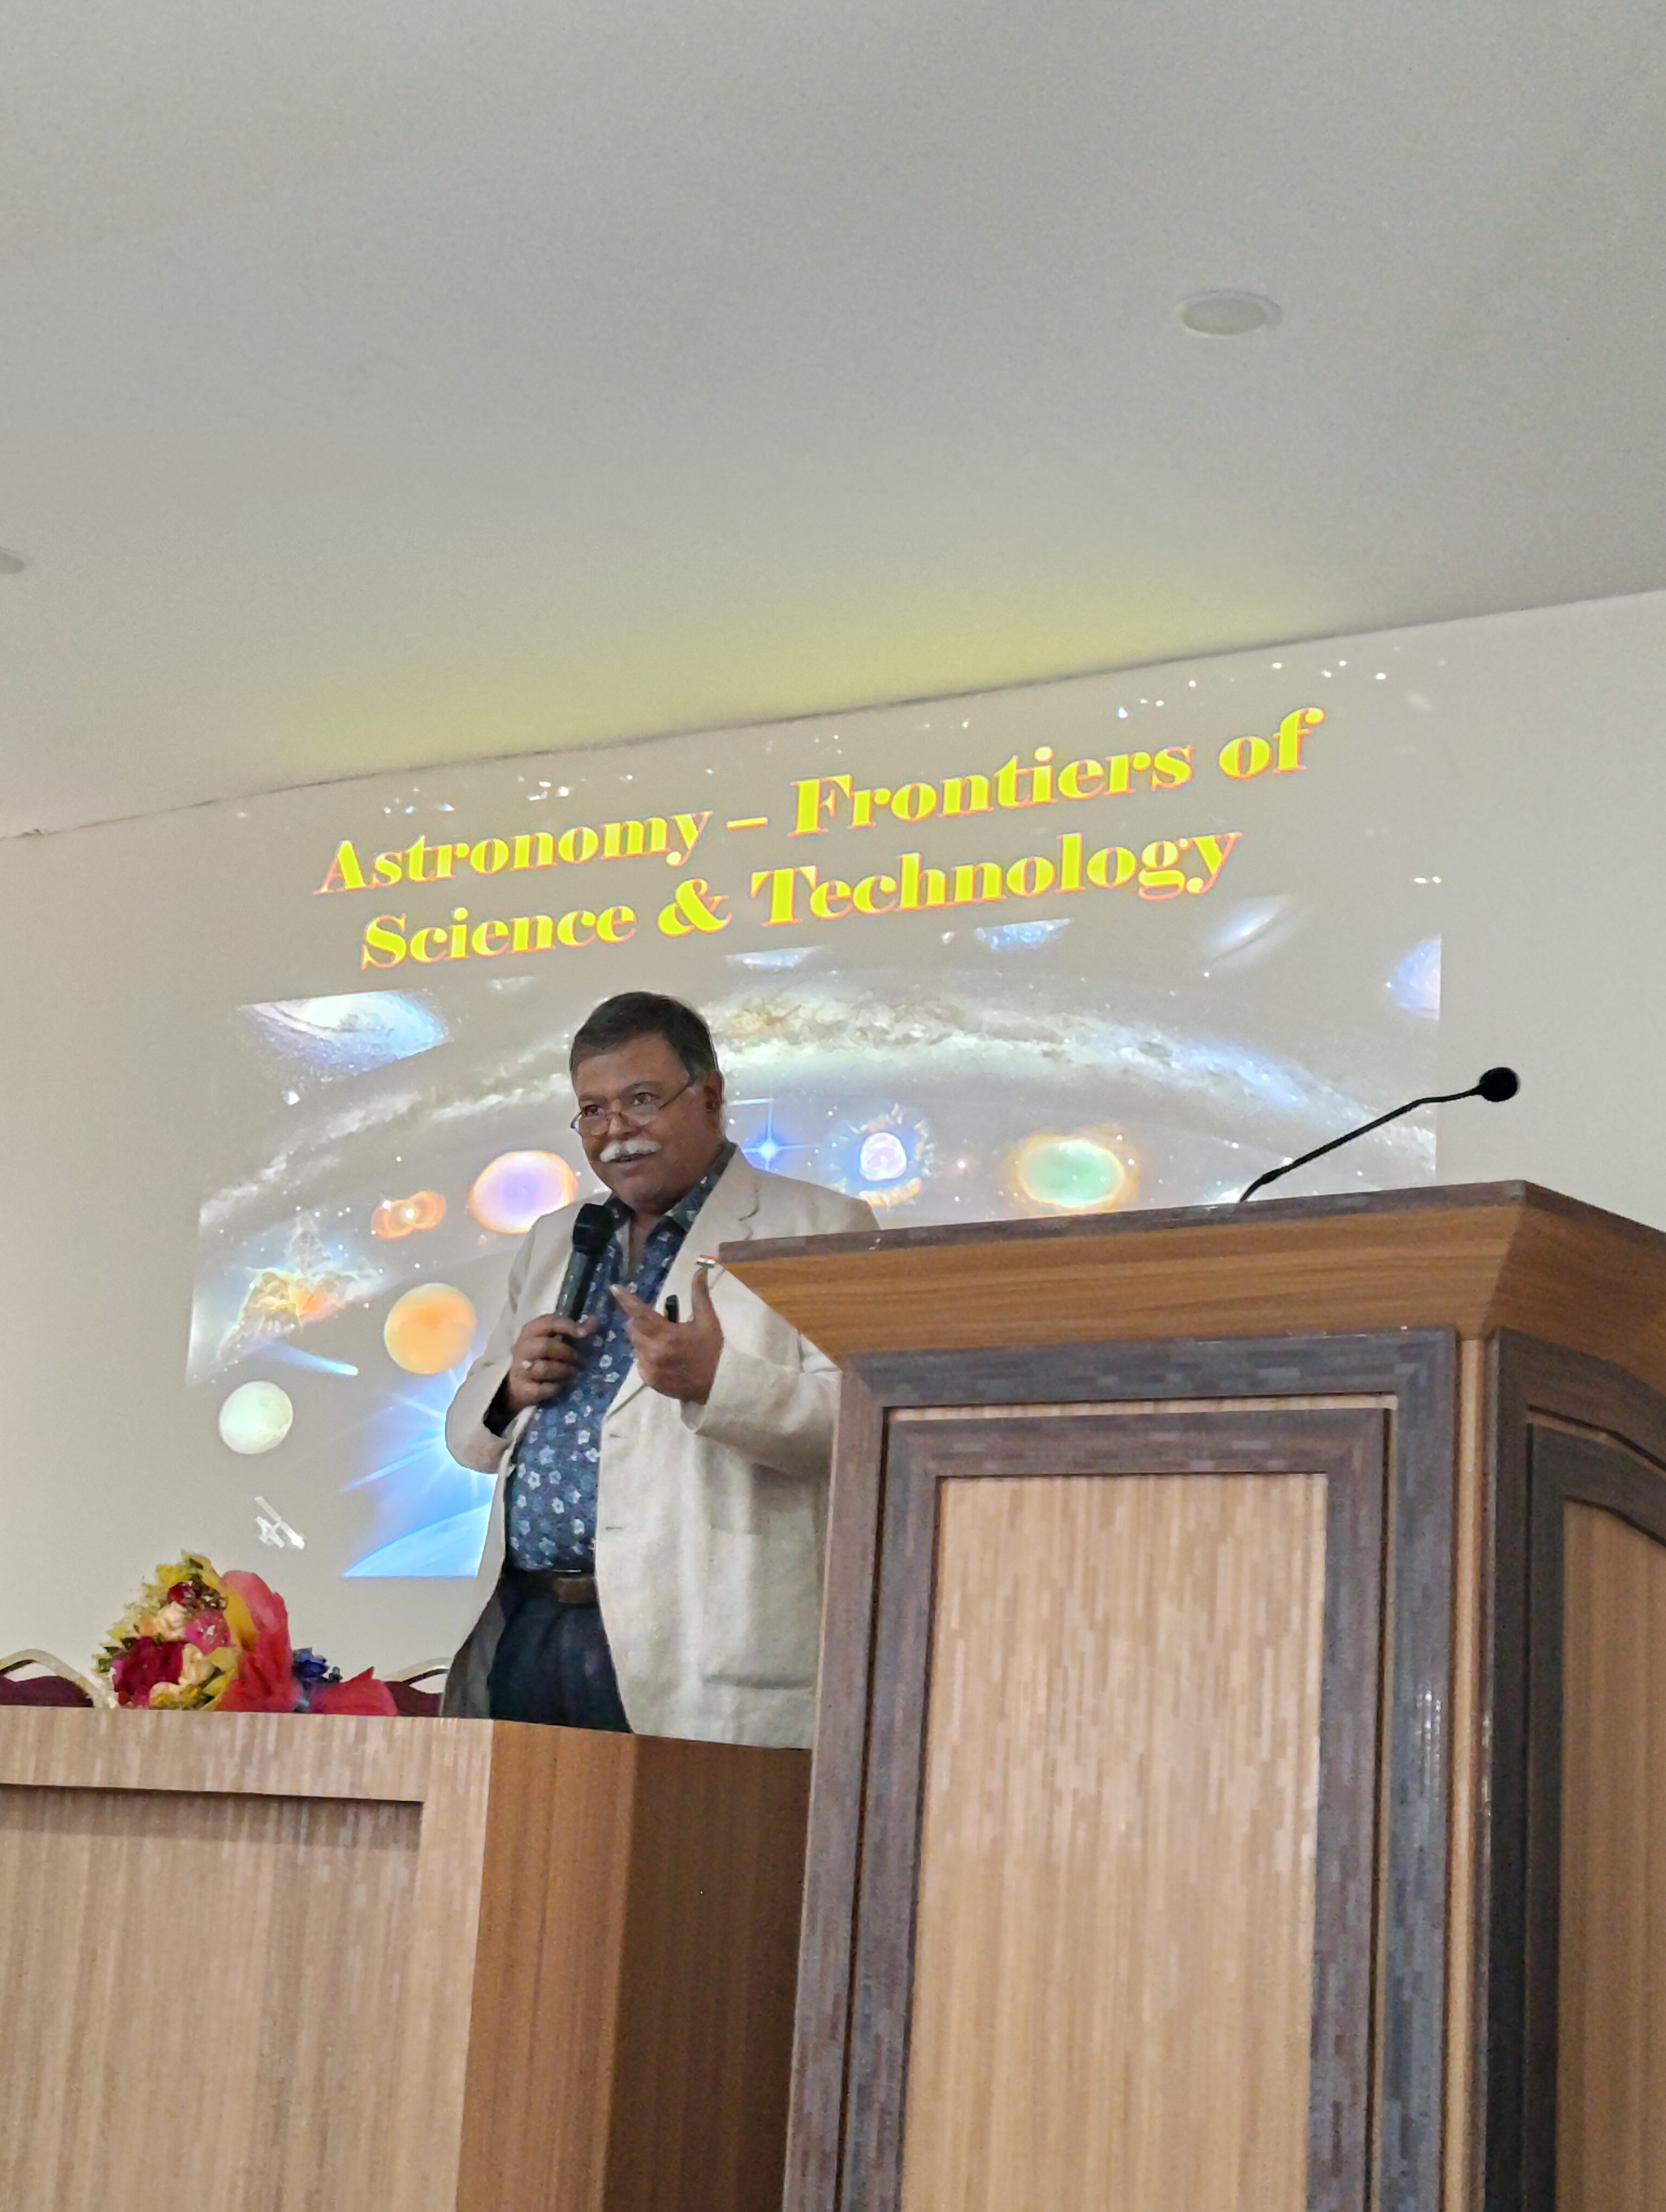
\includegraphics[width=0.4\textwidth]{assets/images/ast-4.jpeg}
  \end{tabular}
\end{center}

{\small
\noindent
\textbf{Kolkata, February 13, 2026---}The scale of the universe met the curiosity of a young engineering audience at St. Thomas' College of Engineering \& Technology (STCET), where renowned astrophysicist Dr. Debiprasad Duari delivered an engaging seminar on ``Astronomy: Frontiers of S\&T.'' Co-organised by the IEEE Computational Intelligence Society (CIS) \& Industrial Electronics Society (IES) Student Chapter, the IEEE Women in Engineering (WIE) Student Branch Affinity Group, and the Institution's Innovation Council (IIC) at STCET, the programme brought students, faculty members and young researchers together for a wide-ranging exploration of modern astronomy and space science.

\medskip
\noindent
Dr. Duari presented astronomy not as a distant catalogue of stars and planets, but as a rapidly advancing field shaped by engineering, computation and international scientific collaboration. His address moved from the familiar architecture of the solar system to the formation of stars and the immense physical processes that govern cosmic phenomena. Complex ideas were communicated in an accessible manner, allowing participants from different academic backgrounds to follow the scientific story without losing sight of its scale or significance.

\medskip
\noindent
A central theme of the session was the convergence of science and technology. Astronomers may begin with fundamental questions---how stars are born, how planetary systems evolve, what lies beyond visible light, and how the universe changes over time---but answering them depends on precision instruments and sophisticated engineering. Telescopes, detectors, satellites, communication links, signal-processing systems, control electronics and large-scale computation have become essential tools for turning faint radiation from space into reliable scientific knowledge.

\medskip
\noindent
The seminar highlighted how each technological advance opens a new observational window. More sensitive detectors reveal objects that earlier instruments could not distinguish; space-based observatories avoid many limitations imposed by Earth's atmosphere; improved electronics allow weak signals to be measured with greater accuracy; and computational methods help researchers process enormous datasets, compare models and identify patterns hidden within noise. The result is a field in which discoveries are often made at the intersection of physics, electronics, communication engineering, data science and intelligent systems.

\medskip
\noindent
Dr. Duari also placed contemporary space exploration within a broader historical transition. The 21st century, he observed, is poised to become a defining period for exploration beyond Earth. Space activity is no longer limited to a small number of national agencies or isolated scientific missions. Universities, research laboratories, start-ups and private companies increasingly contribute instruments, software, small satellites, launch technologies and data-driven services.

\medskip
\noindent
India's growing achievements in space science and technology formed an important part of the discussion. The country's expanding capabilities in launch systems, planetary missions, satellite applications and scientific observation demonstrate how long-term investment in engineering can support both fundamental research and practical national needs. For students, this development creates a widening range of possibilities in spacecraft electronics, remote sensing, communication, navigation, embedded systems, robotics, materials, control engineering and scientific computing.

\medskip
\noindent
The session gained particular energy when the formal lecture opened into an interactive exchange. Students responded with enthusiasm, seeking to connect the ideas presented on stage with questions about the origin and evolution of celestial objects, the limits of present-day observation, future missions and the skills required to enter space-related research. Faculty members and young researchers added questions that linked astronomy with engineering design, computation and interdisciplinary collaboration.

\begin{center}
  \setlength{\tabcolsep}{3pt}
  \begin{tabular}{@{}cc@{}}
    \includegraphics[height=0.35 \textheight]{assets/images/ast-2.jpeg} &
    \includegraphics[height=0.35\textheight]{assets/images/ast-5.jpeg}
  \end{tabular}
\end{center}

\medskip
\noindent
Rather than treating the question-and-answer segment as an appendix to the lecture, Dr. Duari used it to reinforce the method of science itself. Questions that do not yet have complete answers are not failures, the discussion suggested, but starting points for observation, modelling and experiment. The exchange encouraged participants to distinguish established evidence from speculation and to see curiosity as a disciplined habit that must be supported by mathematics, measurement and critical reasoning.

\medskip
\noindent
The audience engagement also demonstrated the value of direct interaction with an experienced science communicator. Astronomy often captures attention through striking images and extraordinary distances, but its deeper educational value lies in the way it unites multiple branches of knowledge. A discussion about a star can involve nuclear physics, spectroscopy, electronics, statistics and computer simulation; a planetary mission can require orbital mechanics, sensors, antennas, autonomous control and reliable software. For engineering students, the field offers a vivid example of why complex problems rarely remain confined to one discipline.

\medskip
\noindent
The participation of the organising bodies reflected that same interdisciplinary outlook. The IEEE CIS \& IES Student Chapter brought perspectives from intelligent computation and industrial electronics, while the IEEE WIE Student Branch Affinity Group reinforced the importance of inclusive participation in science and engineering. The IIC's involvement placed the seminar within the institution's wider effort to promote innovation, research awareness and the translation of ideas into technological possibilities.

\medskip
\noindent
High-calibre scientific talks of this kind can have an impact beyond the duration of a single event. They expose students to research questions that may not appear in a conventional syllabus, introduce possible career pathways and make advanced science feel more approachable. A student initially drawn by the spectacle of space may leave thinking seriously about instrumentation, antenna design, image processing, artificial intelligence, satellite communication or astrophysical research.

\medskip
\noindent
The programme was also a reminder that scientific ambition depends on sustained learning. Space research requires strong foundations, patient experimentation and the willingness to work across disciplinary boundaries. Dr. Duari's accessible presentation encouraged participants to dream boldly while recognising the preparation needed to convert fascination into meaningful study and innovation.

\medskip
\noindent
By the close of the seminar, ``Astronomy: Frontiers of S\&T'' had succeeded in bringing the universe closer to the campus. Its strongest takeaway was not a single fact about a planet or star, but a larger message: cosmic mysteries become answerable when human curiosity is joined with rigorous science, imaginative engineering and technology capable of extending our senses far beyond Earth.

\begin{center}
  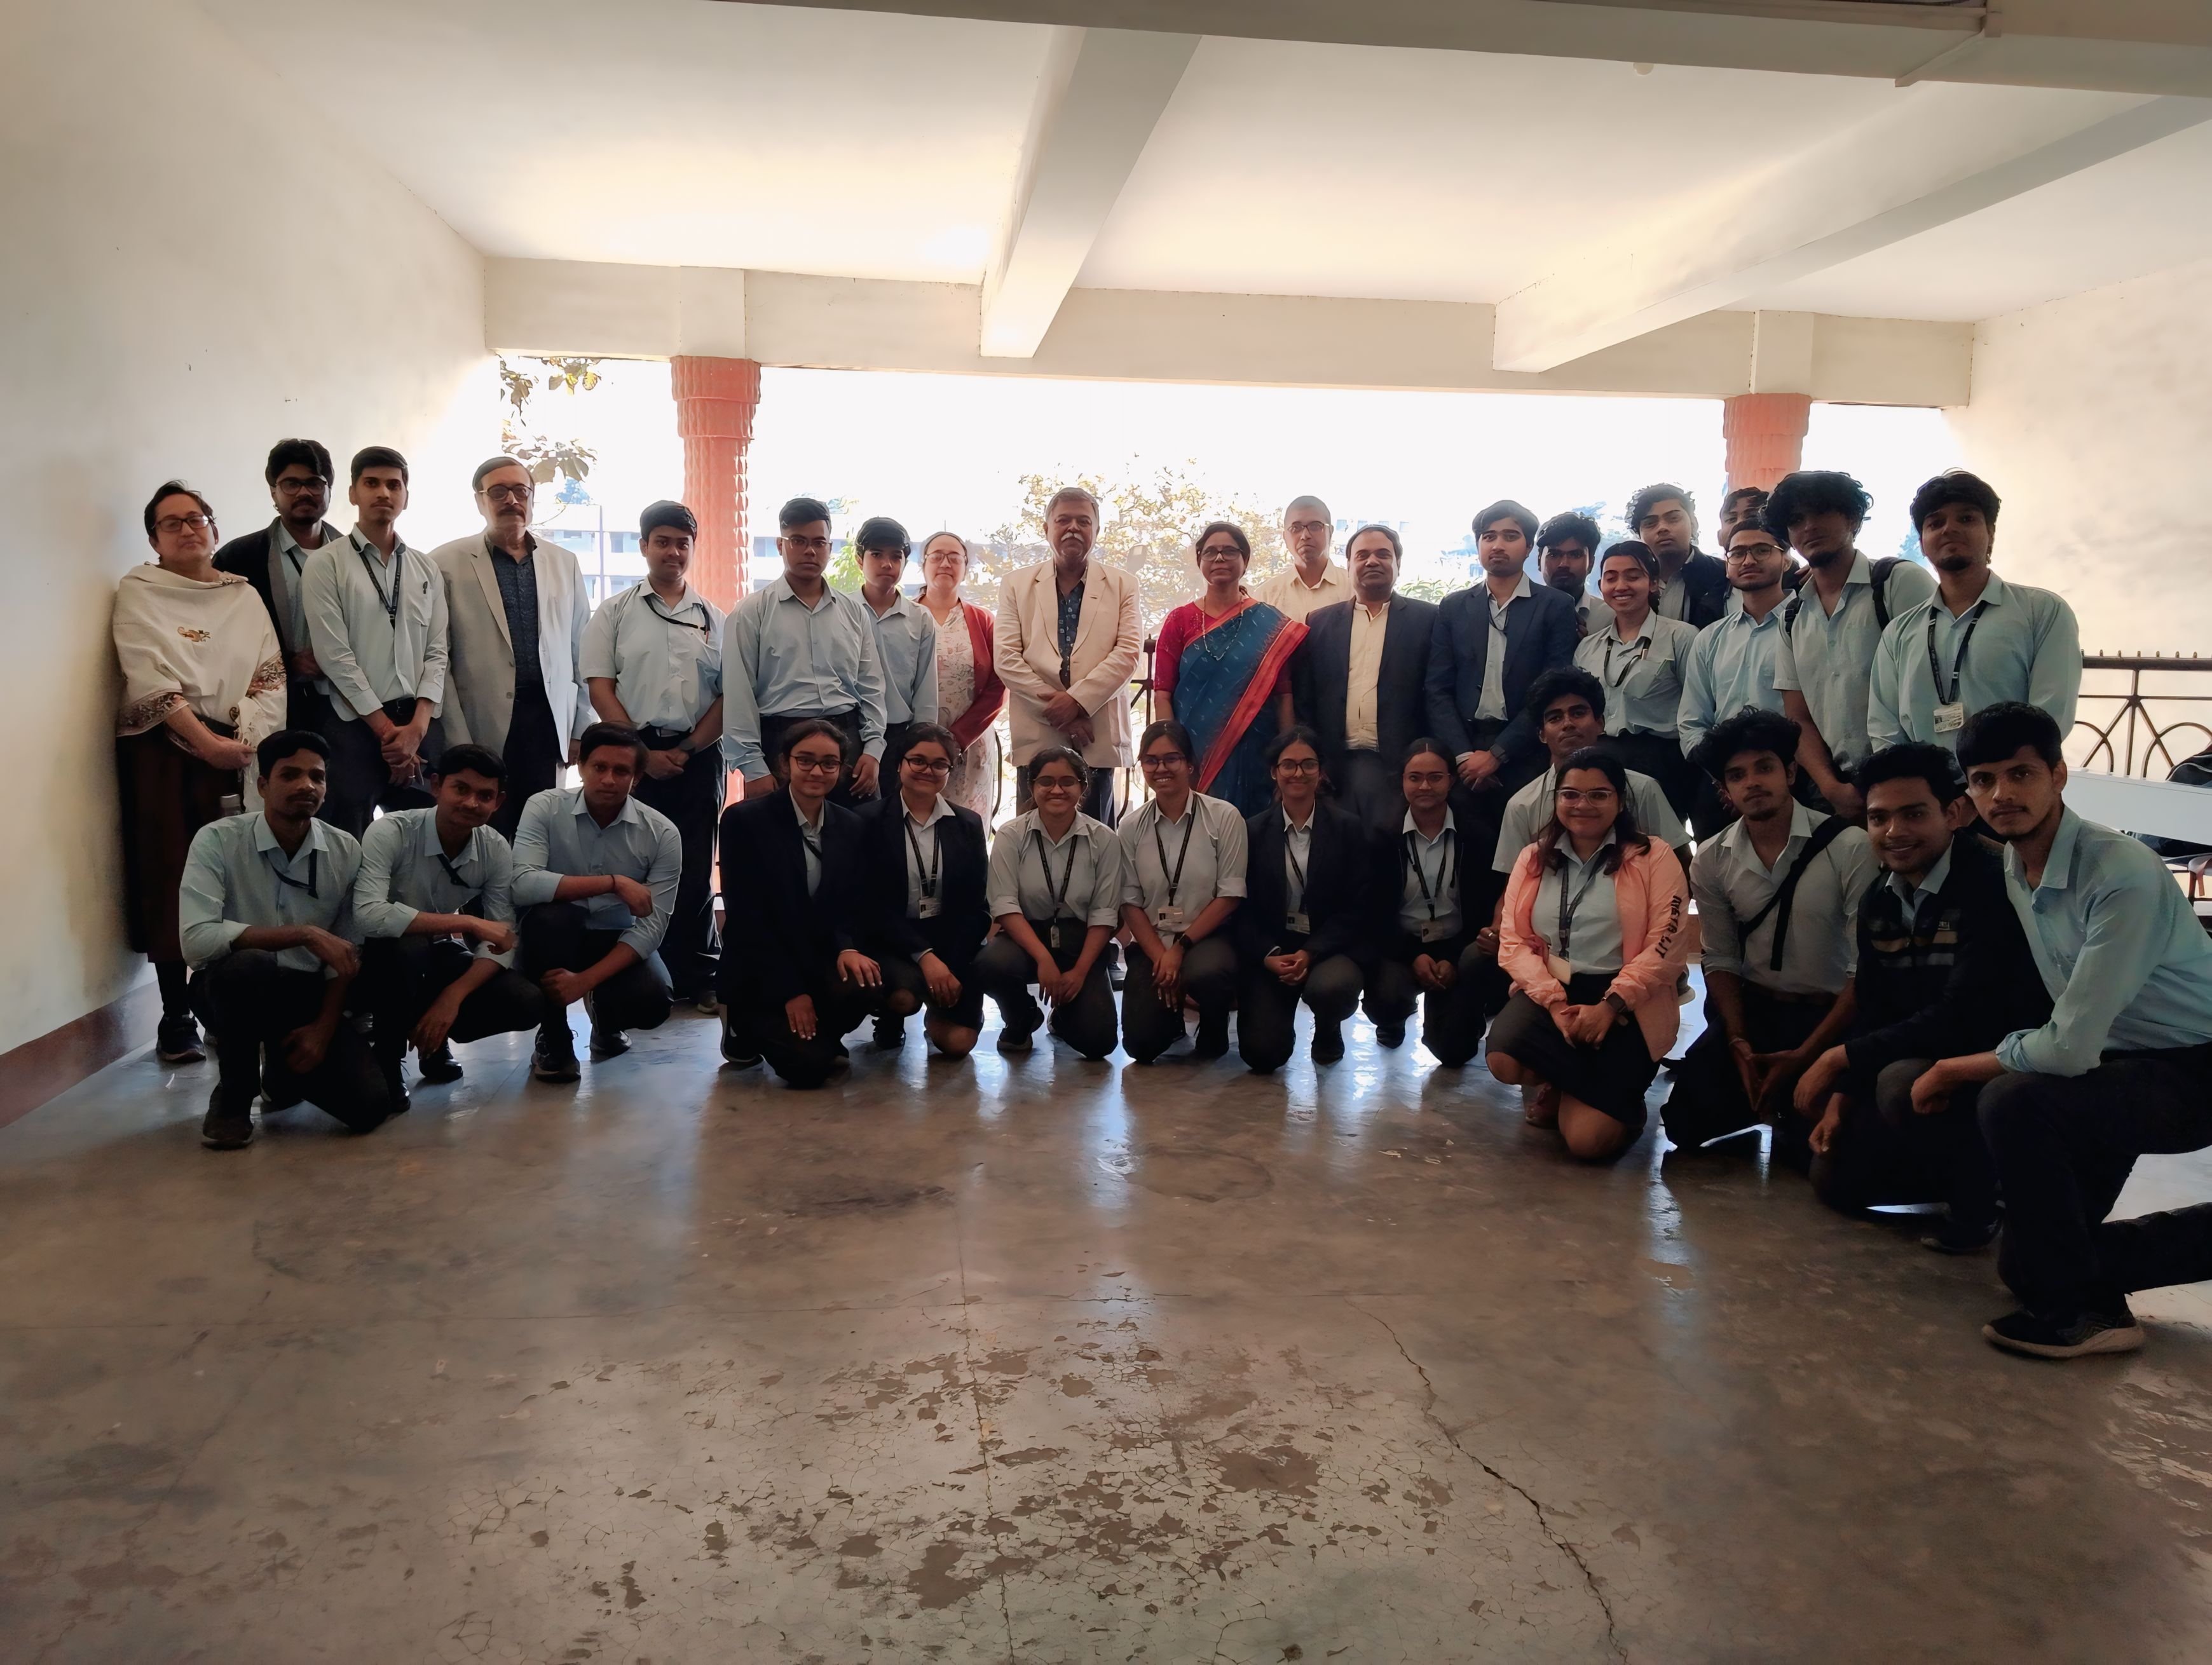
\includegraphics[width=0.8\textwidth]{assets/images/ast-1.jpeg}
\end{center}
\par}

\vfill
\noindent
{\footnotesize\sloppy\textit{Source note: The event theme, organisers and interactive format are based on the programme brief. Key lecture themes are supported by a published account of Dr. Duari's STCET address, which described his discussion of the solar system, star formation, cosmic phenomena, India's space achievements and the future of exploration.}\par}

\newpage
\addcontentsline{toc}{subsection}{AI, Autonomy and Swarming at STCET}
\begin{center}
  {\LARGE\bfseries Prof. Debasish Ghose Maps the Future of AI, Autonomy and Swarming at STCET\par}
  \vspace{0.45em}
  {\large\bfseries\color{IEEEblue}
  IISc aerospace expert links multi-robot intelligence with defence, deep-space navigation and the next generation of scientific missions.\par}
  \vspace{0.5em}
  {\small\itshape By the Editorial Desk}
\end{center}

\begin{tcolorbox}[
  colback=SoftBlue,
  colframe=IEEEblue!75!black,
  boxrule=0.6pt,
  arc=0mm,
  left=3mm,right=3mm,top=2mm,bottom=2mm
]
  \small\RaggedRight
  \textbf{At a glance:} Prof. Debasish Ghose of the Department of Aerospace Engineering, Indian Institute of Science (IISc), Bengaluru, delivered the technical talk ``Towards Innovation on AI, Autonomy and Swarming'' at noon on February 16, 2026, in the STCET Seminar Hall. The programme was organised by the IEEE Student Branch--STCET with the IEEE CIS \& IES Student Chapter, IEEE WIE Student Branch Affinity Group, Institution's Innovation Council (IIC), and Research \& Development Cell, STCET.
\end{tcolorbox}

\begin{center}
  \setlength{\tabcolsep}{2pt}
  \begin{tabular}{@{}cc@{}}
    \includegraphics[height=0.4\textheight]{assets/images/aas-2.jpeg} &
    \includegraphics[height=0.4\textheight]{assets/images/aas3.jpeg}
  \end{tabular}

  \vspace{2pt}
  {\footnotesize\itshape Speakers introduce the technical session on AI, autonomy and swarming.\par}
\end{center}

{\small
\noindent
\textbf{Kolkata, February 16, 2026---}Artificial intelligence moved from the screen into the physical world during a distinguished technical talk at St. Thomas' College of Engineering \& Technology (STCET), where Prof. Debasish Ghose of IISc Bengaluru examined how autonomous machines can navigate, cooperate and make decisions as a group. The session on ``Towards Innovation on AI, Autonomy and Swarming'' was jointly supported by the IEEE CIS \& IES Student Chapter, the IEEE WIE Student Branch Affinity Group, the Institution's Innovation Council (IIC), and the Research \& Development Cell, STCET, under the IEEE Student Branch.

\medskip
\noindent
Prof. Ghose, whose research centres on the guidance and control of autonomous vehicles, introduced the audience to a field reshaping aerospace engineering, robotics and intelligent defence systems. His central message was that autonomy is more than automation. An automated machine follows a predetermined sequence; an autonomous system must sense its surroundings, interpret incomplete information, choose a course of action and adjust when conditions change.

\medskip
\noindent
That distinction becomes especially important when several robots or vehicles work together. A multi-robot system can divide a large task among many relatively simple agents, allowing the group to search a wider area, respond from multiple directions and continue operating even if one member fails. The engineering challenge is to coordinate the agents without creating excessive communication, computation or dependence on a single controller.

\medskip
\noindent
The lecture used swarm intelligence to explain how local decisions can produce useful collective behaviour. Natural swarms offer familiar examples: individual birds, insects or fish respond mainly to nearby neighbours, yet the group can move cohesively, avoid obstacles and adapt to threats. In engineered swarms, carefully designed algorithms translate similar principles into rules for alignment, separation, formation, task allocation, consensus and cooperative search.

\medskip
\noindent
Prof. Ghose highlighted that effective swarm behaviour does not emerge from imitation alone. Each agent requires sensing, localisation, communication and control, while the group needs algorithms that remain stable when information is delayed, noisy or incomplete. Designers must decide how much intelligence belongs on each vehicle, what information should be shared, and how the system should respond when communication links disappear or an agent behaves unexpectedly.

\begin{center}
  \setlength{\tabcolsep}{2pt}
  \begin{tabular}{@{}cc@{}}
    \includegraphics[height=0.4\textheight]{assets/images/aas-4.jpeg} &
    \includegraphics[height=0.4\textheight]{assets/images/aas-5.jpeg}
  \end{tabular}

  \vspace{2pt}
  {\footnotesize\itshape Moments from the lecture and the felicitation of the invited speaker.\par}
\end{center}

\medskip
\noindent
Dynamic path planning formed another major strand of the discussion. Unlike route planning on a fixed map, autonomous navigation often takes place in environments that change while a mission is under way. Obstacles may move, weather may deteriorate, targets may shift and new information may arrive from other agents. A practical planner must continually update a route while respecting constraints such as energy, turning radius, collision risk, sensor range and mission priority.

\medskip
\noindent
For a single vehicle, these requirements are already demanding. For a swarm, path planning becomes a coupled problem: every agent must make progress toward the mission objective without colliding with teammates or duplicating work unnecessarily. Distributed algorithms can allow vehicles to negotiate roles, maintain formations, exchange local observations and reassign tasks when circumstances change. The result is a system whose capability comes from coordination rather than from one exceptionally powerful machine.

\medskip
\noindent
The aerospace and defence relevance of these ideas was evident throughout the talk. Groups of unmanned aerial vehicles can support wide-area surveillance, disaster assessment, mapping, search operations and inspection of hazardous regions. Cooperative systems can cover terrain faster than a single platform, observe an object from several viewpoints and maintain a mission despite individual failures. Similar principles can guide marine robots, ground vehicles and mixed teams operating across air, land and water.

\medskip
\noindent
Prof. Ghose also connected autonomous swarms with the challenges of space exploration and astronomical observation. Satellite constellations increasingly depend on coordinated scheduling, relative positioning and communication across many spacecraft. Instead of treating each satellite as an isolated platform, autonomy can help a constellation distribute observations, manage resources and respond to changing mission priorities with less continuous intervention from the ground.

\medskip
\noindent
Deep-space missions create an even stronger case for onboard intelligence. Communication delays make immediate human control impossible when a spacecraft or planetary robot is far from Earth. Autonomous navigation must combine sensor data, estimate position, detect hazards and select safe actions locally. A group of small robotic explorers could potentially survey a larger planetary region, share discoveries and redirect one another toward scientifically important targets.

\begin{center}
  \setlength{\tabcolsep}{2pt}
  \begin{tabular}{@{}cc@{}}
    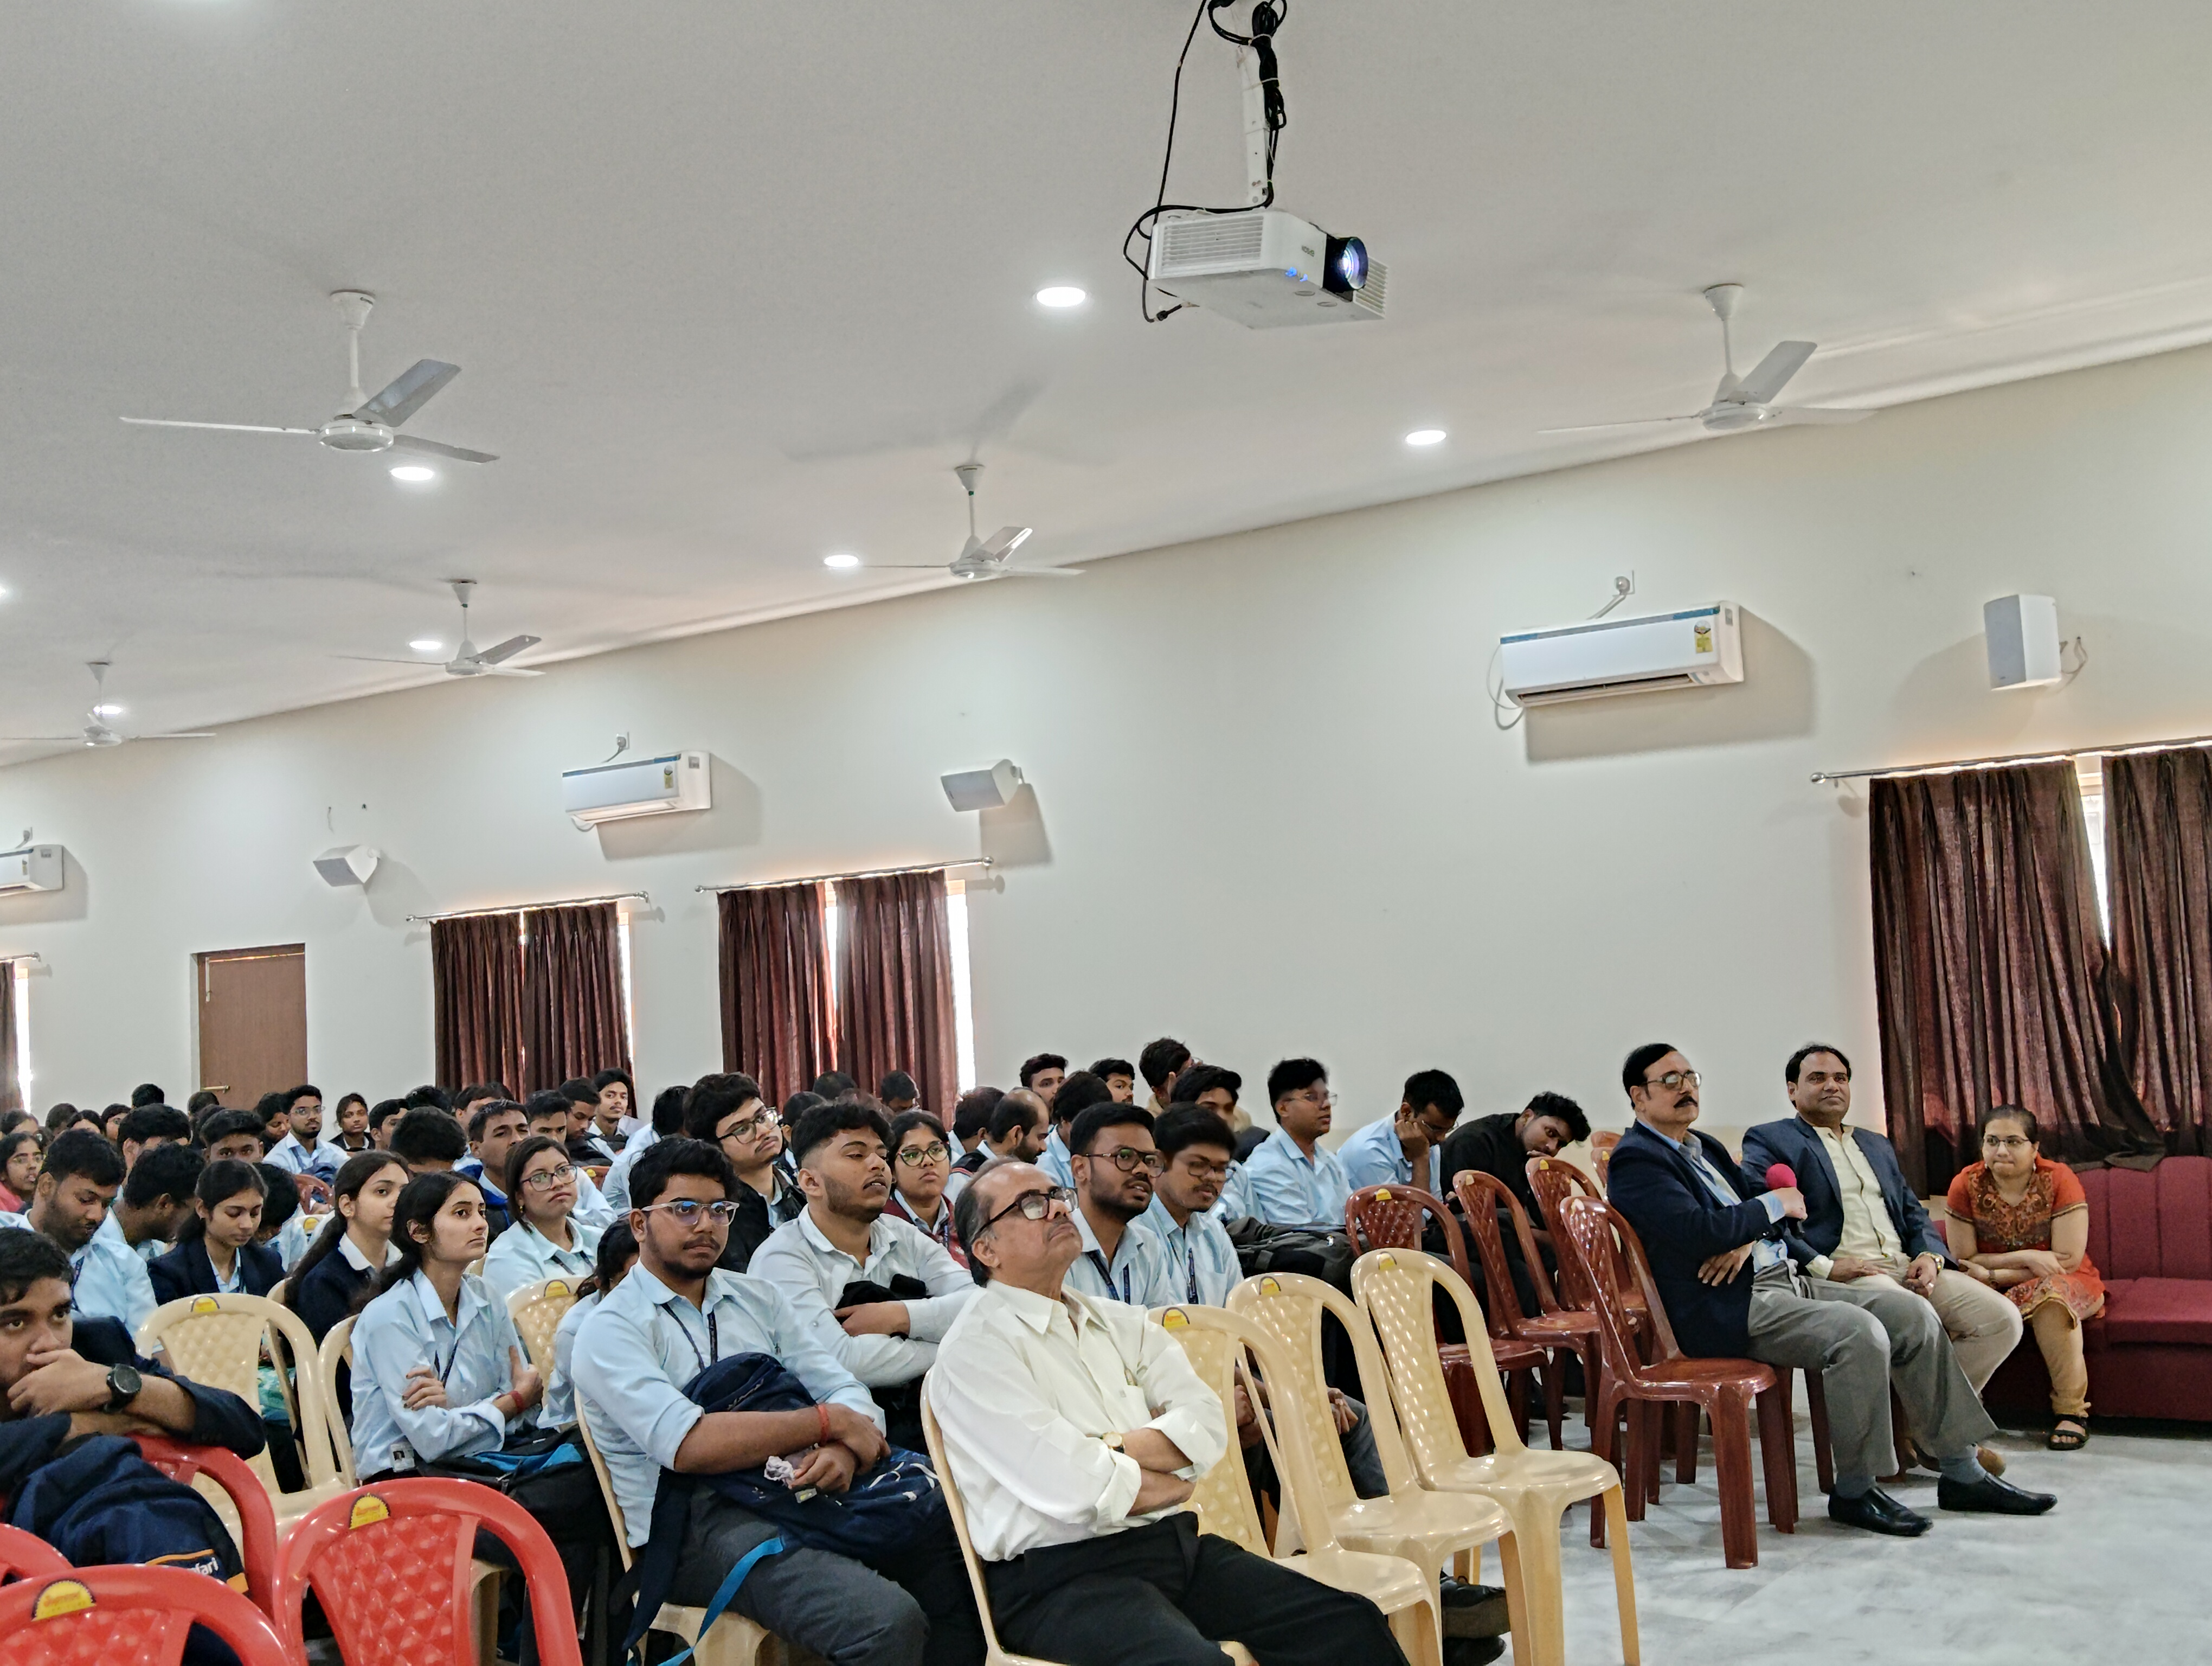
\includegraphics[width=0.45\textwidth]{assets/images/aas-6.jpeg} &
    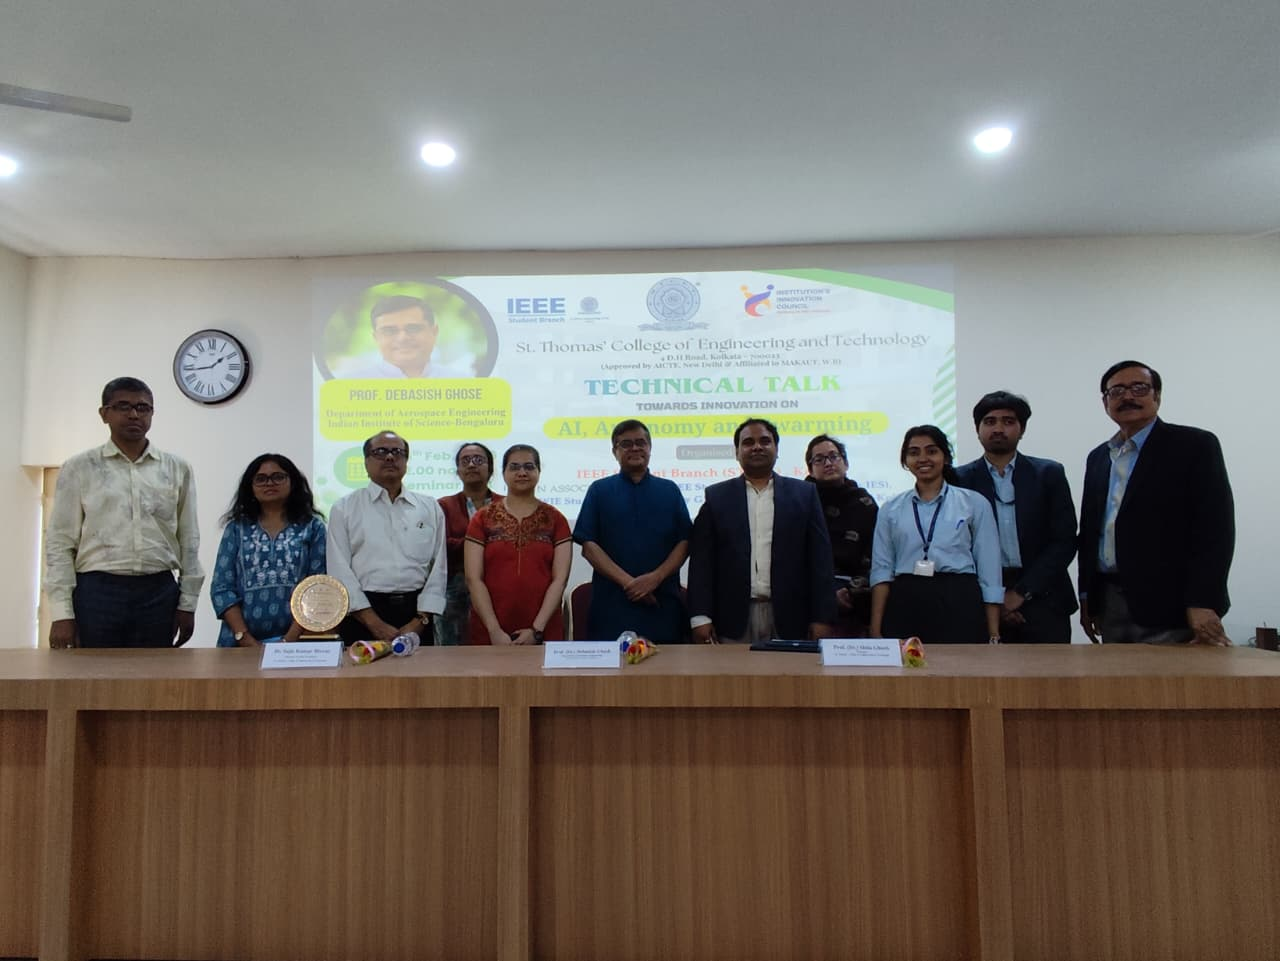
\includegraphics[width=0.45\textwidth]{assets/images/aas-7.jpeg}
  \end{tabular}

  \vspace{2pt}
  {\footnotesize\itshape The attentive audience and organisers at the conclusion of the programme.\par}
\end{center}

\medskip
\noindent
In astronomical missions, coordinated spacecraft can observe the same phenomenon from different locations or divide a survey among several instruments. Swarming concepts could support distributed sensing, formation flying and interferometric observations in which measurements from separated platforms are combined. Such missions demand extraordinary precision: small navigation or timing errors can degrade the scientific result, making guidance, synchronisation and fault-tolerant control as important as the telescope or detector itself.

\medskip
\noindent
The lecture balanced this technological promise with the limits that engineers must confront. Autonomous systems can fail because of poor training data, sensor errors, unforeseen conditions, cyberattack or an objective function that does not reflect the real mission. In defence and other safety-critical applications, decisions may also carry ethical and legal consequences. Human oversight, explainability, secure communication, testing and clearly defined authority therefore remain essential even as machines gain greater independence.

\medskip
\noindent
These concerns carried into the interactive question-and-answer session. Students, IEEE members and faculty participants engaged Prof. Ghose on the trustworthiness of AI decisions, the balance between centralised and distributed control, and the difficulty of guaranteeing safe collective behaviour. Questions also explored how engineers can prevent a swarm from amplifying one faulty decision across the entire group.

\medskip
\noindent
Young researchers sought guidance on entering the field, prompting discussion of the foundations required for meaningful work in autonomy: mathematics, control theory, optimisation, programming, robotics, probability, signal processing and machine learning. The exchange made clear that autonomous-systems research is inherently interdisciplinary. Progress depends on researchers who can connect algorithms with sensors, actuators, communication limits and the physical dynamics of real vehicles.

\medskip
\noindent
The programme's joint organisation reflected this breadth. The IEEE CIS community contributed the perspective of computational intelligence; the IES chapter connected intelligent algorithms with electronics and industrial systems; IEEE WIE reinforced inclusive participation in advanced technology; and the IIC and R\&D Cell placed the discussion within STCET's wider culture of innovation and research.

\medskip
\noindent
For students, the talk offered more than a survey of an emerging field. It showed how concepts learned separately in classrooms---feedback control, embedded systems, communication networks, optimisation and AI---come together in machines that must act reliably in the real world. It also demonstrated why research problems at the frontier rarely belong to one department or one branch of engineering.

\medskip
\noindent
By the close of the session, autonomy had been presented neither as effortless machine intelligence nor as a distant futuristic idea. It emerged as a demanding engineering discipline built on models, evidence, careful testing and responsible design. Prof. Ghose's talk left the audience with a compelling picture of the future: fleets of machines capable of cooperating across Earth and space, provided that human ingenuity is matched by technical rigour and ethical judgement.
\par}

\begin{center}
  \includegraphics[width=\textwidth]{assets/images/aas-1.jpeg}

  \vspace{2pt}
  {\footnotesize\itshape The technical talk in progress at the STCET Seminar Hall.\par}
\end{center}

\vfill
\noindent
{\footnotesize\sloppy\textit{Source note: Event title, date, time, venue and organising details are based on the official STCET event listing and programme announcement. Professional details are based on the official IISc Aerospace Engineering profile of Prof. Debasish Ghose.}\par}
\thispagestyle{empty}
\vspace*{\fill}
\addcontentsline{toc}{section}{Fun Zone}
\begin{center}
    \section*{\normalfont\rmfamily\cursive\fontsize{60}{72}\selectfont Fun Zone}
\end{center}
\vspace*{\fill}

\newpage

\begin{center}
  {\LARGE\bfseries\rmfamily\color{IEEEblue} Electronics Crossword\par}
  \vspace{0.2em}
  {\small\itshape Test your knowledge of circuits, logic and electronic devices.\par}
  \vspace{0.6em}
  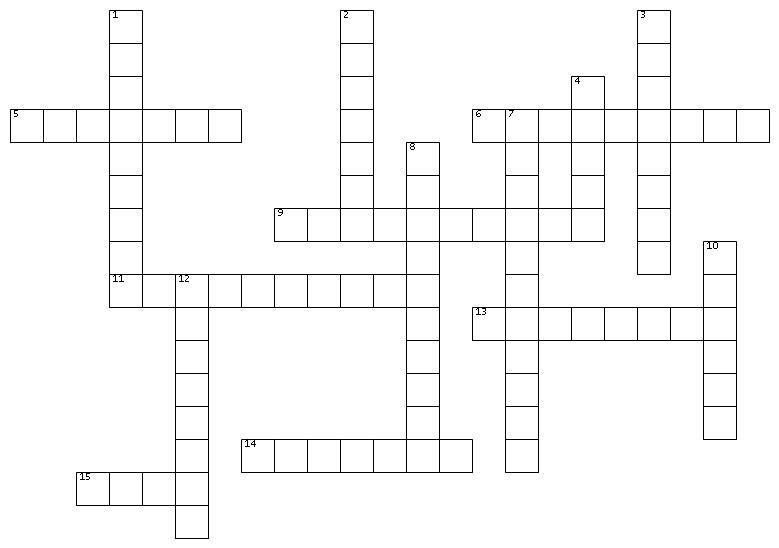
\includegraphics[width=0.94\textwidth]{assets/images/ecrossword.png}
\end{center}

\vspace{0.5em}
\noindent
\begin{minipage}[t]{0.485\textwidth}
  {\large\bfseries\rmfamily\color{IEEEblue} ACROSS}\par
  \vspace{0.2em}
  {\color{IEEEorange}\rule{\linewidth}{1pt}}\par
  \smallskip
  \footnotesize
  \begin{enumerate}[leftmargin=2.1em,itemsep=3pt,topsep=0pt,parsep=0pt]
    \item[\textbf{5.}] Voltage reference circuit that provides a stable output independent of temperature
    \item[\textbf{6.}] Total opposition a circuit offers to alternating current at a given frequency
    \item[\textbf{9.}] Passive device used to reduce the power of a signal without distorting its waveform
    \item[\textbf{11.}] Lagging of an effect behind its cause seen in Schmitt triggers
    \item[\textbf{13.}] Bistable multivibrator used as a basic memory element to store one bit
    \item[\textbf{14.}] Combinational circuit that converts multiple input lines into a coded binary output
    \item[\textbf{15.}] Term for a circuit node that absorbs current coming from a load
  \end{enumerate}
\end{minipage}%
\hfill
\begin{minipage}[t]{0.485\textwidth}
  {\large\bfseries\rmfamily\color{IEEEblue} DOWN}\par
  \vspace{0.2em}
  {\color{IEEEorange}\rule{\linewidth}{1pt}}\par
  \smallskip
  \footnotesize
  \begin{enumerate}[leftmargin=2.1em,itemsep=3pt,topsep=0pt,parsep=0pt]
    \item[\textbf{1.}] Difference between the upper and lower frequencies in a continuous band of signals
    \item[\textbf{2.}] Trigger circuit that uses positive feedback to clean up noisy input signals
    \item[\textbf{3.}] Voltage-variable capacitor diode used in RF tuning circuits
    \item[\textbf{4.}] Special diode designed to reliably allow current to flow backwards when a specific reverse voltage is reached
    \item[\textbf{7.}] Combinational logic circuit that selects one of several input signals and forwards it to a single line
    \item[\textbf{8.}] Multivibrator circuit that produces a single output pulse when triggered
    \item[\textbf{10.}] Small unwanted residual AC voltage remaining after rectification
    \item[\textbf{12.}] Fast-switching diode featuring a low forward voltage drop
  \end{enumerate}
\end{minipage}

\newpage

\begin{center}
  {\LARGE\bfseries\rmfamily\color{IEEEblue} Circuit Seekers\par}
  \vspace{0.15em}
  {\large\bfseries\rmfamily Electronics Word Search\par}
  \vspace{0.2em}
  {\small\itshape Find the hidden terms from electronics, communication and semiconductor engineering.\par}

  \vspace{1em}
  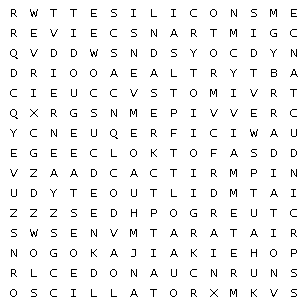
\includegraphics[width=0.9\textwidth]{assets/images/ewordsearch.png}

  \vspace{1em}
  {\large\bfseries\rmfamily\color{IEEEblue} WORD BANK}\par
  \vspace{0.2em}
  {\color{IEEEorange}\rule{0.94\textwidth}{1pt}}\par
  \vspace{0.6em}

  \footnotesize\rmfamily
  \setlength{\tabcolsep}{8pt}
  \renewcommand{\arraystretch}{1.35}
  \begin{tabular}{@{}llll@{}}
    MICROPROCESSOR & DRAIN         & MODULATION     & AMMETER \\
    FREQUENCY      & SOURCE        & MULTIVIBRATOR  & CONDUCTOR \\
    CAPACITANCE    & ANODE         & FLIPFLOP       & INSULATOR \\
    INDUCTANCE     & CATHODE       & ENCODER        & SEMICONDUCTOR \\
    CONDUCTIVITY   & AMPLIFIER     & DECODER        & PHOTODIODE \\
    SILICON        & OSCILLATOR    & COMPARATOR     & TRANSDUCTOR \\
    GATE           & WAVEFORM      & REGULATOR      & TRANSMISSION \\
    HARMONICS      & ATTENUATION   & VOLTMETER      & SENSITIVITY \\
    RADIATION      & POLARIZATION  & GAIN           & RECTIFICATION \\
    TRANSCEIVER    & DEMODULATOR   & THERMISTOR     & VARISTOR
  \end{tabular}
\end{center}

\newpage

\begin{center}
  {\LARGE\bfseries\rmfamily\color{IEEEblue} Circuit Brain Teasers\par}
  \vspace{0.2em}
  {\small\itshape Who am I? Identify each electronic device, concept or architecture.\par}
\end{center}

\vspace{0.7em}
\begin{tcolorbox}[
  colback=black!2,
  colframe=IEEEblue!75!black,
  boxrule=0.6pt,
  arc=0mm,
  left=5mm,
  right=5mm,
  top=4mm,
  bottom=4mm
]
  \small
  \begin{enumerate}[leftmargin=2.1em,itemsep=0.75em,topsep=0pt,parsep=0pt]
    \item I am a specialized antenna whose physical geometry contains radio frequency switches. By turning those switches on or off, I can instantly alter my operating frequency, radiation pattern, or polarization on the fly. Who am I?

    \item I contain an ALU, control unit, and registers on a single integrated circuit, serving as the central engine that fetches, decodes, and executes instructions line by line. Who am I?

    \item I consist of multiple individual radiating elements fed with specific phase delays, allowing me to steer a narrow electromagnetic beam electronically without moving a single part. Who am I?

    \item I sit right next to the processor core, operating at near-CPU speeds. I store copies of frequently accessed RAM data so the execution unit never starves waiting for memory access. Who am I?

    \item I stack multiple antenna elements together using specialized spatial arrangements to drastically increase channel capacity and link reliability over an ultra-wide frequency spectrum. Who am I?

    \item I am an architecture technique where multiple instruction steps---fetch, decode, execute, writeback---are overlapped in parallel stages, drastically boosting clock-cycle efficiency. Who am I?

    \item I am a microstrip planar antenna featuring a flat metal patch printed on top of a dielectric substrate above a ground plane, widely used for compact wireless applications. Who am I?

    \item I am a physical pin on a microprocessor. When a peripheral pulls my voltage line, I force the CPU to immediately suspend its current code execution and run a specialized handler routine. Who am I?

    \item I am a ratio that measures how efficiently radio frequency power is transmitted from a feedline into an antenna, reaching an ideal value of 1:1 when there are no reflected standing waves. Who am I?

    \item I am a specialized register inside a microprocessor that holds the memory address of the very next instruction waiting to be fetched and executed. Who am I?
  \end{enumerate}
\end{tcolorbox}

\vfill
\begin{center}
  {\small\bfseries\rmfamily\color{IEEEblue}
  Answers to the Fun Zone puzzles are given on the next page.\par}
\end{center}

\thispagestyle{empty}
\addcontentsline{toc}{section}{Fun Zone — Answers}
\begin{center}
  {\LARGE\bfseries\rmfamily\color{IEEEblue} Fun Zone — Answers\par}
  \vspace{0.2em}
  {\small\itshape Solutions to the Electronics Crossword, Word Search and Circuit Brain Teasers.\par}
  \vspace{0.5em}
  {\color{IEEEorange}\rule{0.92\textwidth}{1pt}}\par
\end{center}

\vspace{0.6em}

% ---------- CROSSWORD ----------
\begin{tcolorbox}[
  colback=SoftBlue,
  colframe=IEEEblue!70!black,
  boxrule=0.5pt,
  arc=0mm,
  left=4mm, right=4mm, top=3mm, bottom=3mm
]
{\large\bfseries\rmfamily\color{IEEEblue} 1. Electronics Crossword — Solutions\par}
\vspace{0.15em}
{\color{IEEEorange}\rule{\linewidth}{0.8pt}}\par
\smallskip
\footnotesize\rmfamily
\noindent The crossword grid on page 104 is filled as below. Letters run left-to-right (Across) and top-to-bottom (Down). The word list matches the clues exactly.

\medskip
\noindent
\begin{minipage}[t]{0.485\textwidth}
  {\small\bfseries\rmfamily\color{IEEEblue} ACROSS}\par
  \vspace{0.15em}
  {\color{black!15}\hrule height 0.4pt}\par
  \smallskip
  \begin{enumerate}[leftmargin=1.8em,itemsep=2pt,topsep=0pt,parsep=0pt, label=\textbf{\arabic*.}]
    \item[\textbf{5.}] \textbf{BANDGAP} — Bandgap reference (e.g., Brokaw) gives $\sim$1.22\,V stable with temperature.
    \item[\textbf{6.}] \textbf{IMPEDANCE} — $Z = R + jX$, magnitude $|Z|$ at a frequency.
    \item[\textbf{9.}] \textbf{ATTENUATOR} — Resistive T/$\Pi$ pad, reduces power without distortion.
    \item[\textbf{11.}] \textbf{HYSTERESIS} — Memory in Schmitt transfer, upper/lower thresholds.
    \item[\textbf{13.}] \textbf{FLIPFLOP} — RS/JK/D bistable, stores 1 bit.
    \item[\textbf{14.}] \textbf{ENCODER} — $n$ lines → $m$ bits (e.g., 8:3).
    \item[\textbf{15.}] \textbf{SINK} — Current sink (opposite of source).
  \end{enumerate}
\end{minipage}%
\hfill
\begin{minipage}[t]{0.485\textwidth}
  {\small\bfseries\rmfamily\color{IEEEblue} DOWN}\par
  \vspace{0.15em}
  {\color{black!15}\hrule height 0.4pt}\par
  \smallskip
  \begin{enumerate}[leftmargin=1.8em,itemsep=2pt,topsep=0pt,parsep=0pt, label=\textbf{\arabic*.}]
    \item[\textbf{1.}] \textbf{BANDWIDTH} — $BW = f_H - f_L$.
    \item[\textbf{2.}] \textbf{SCHMITT TRIGGER} — Schmitt trigger, positive feedback cleans noisy edges.
    \item[\textbf{3.}] \textbf{VARACTOR} — Varactor / varicap, $C(V)$ for VCOs/tuning.
    \item[\textbf{4.}] \textbf{ZENER} — Zener diode, reverse breakdown at $V_Z$.
    \item[\textbf{7.}] \textbf{MULTIPLEXER} — MUX, $2^n$:1 selector.
    \item[\textbf{8.}] \textbf{MONOSTABLE} — Monostable / one-shot, single pulse $T\approx0.33RC$.
    \item[\textbf{10.}] \textbf{RIPPLE} — Ripple, e.g., 100\,Hz after full-wave rectifier.
    \item[\textbf{12.}] \textbf{SCHOTTKY} — Schottky diode, $\sim$0.2–0.3\,V $V_F$, fast recovery.
  \end{enumerate}
\end{minipage}

\medskip
\footnotesize\itshape Note: 2-Down and 11-Across both refer to the Schmitt hysteresis effect; grid places \texttt{SCHMITT} vertically and \texttt{HYSTERESIS} horizontally, intersecting at the `H`.
\end{tcolorbox}

\vspace{0.5em}

% ---------- WORD SEARCH ----------
\begin{tcolorbox}[
  colback=white,
  colframe=IEEEblue!70!black,
  boxrule=0.5pt,
  arc=0mm,
  left=4mm, right=4mm, top=3mm, bottom=3mm
]
{\large\bfseries\rmfamily\color{IEEEblue} 2. Circuit Seekers — Word Search Solutions\par}
\vspace{0.15em}
{\color{IEEEorange}\rule{\linewidth}{0.8pt}}\par
\smallskip
\footnotesize\rmfamily
\noindent All 40 words from the bank on page 105 are hidden in the grid on page 105 (horizontal, vertical and diagonal, forward and backward). The solved grid is the same artwork with each word highlighted.

\medskip
\scriptsize\rmfamily
\setlength{\tabcolsep}{6pt}
\renewcommand{\arraystretch}{1.25}
\begin{tabular}{@{}llll@{}}
  \textcolor{IEEEblue}{\textbf{MICROPROCESSOR}} & \textcolor{IEEEblue}{\textbf{DRAIN}} & \textcolor{IEEEblue}{\textbf{MODULATION}} & \textcolor{IEEEblue}{\textbf{AMMETER}} \\
  \textcolor{IEEEblue}{\textbf{FREQUENCY}} & \textcolor{IEEEblue}{\textbf{SOURCE}} & \textcolor{IEEEblue}{\textbf{MULTIVIBRATOR}} & \textcolor{IEEEblue}{\textbf{CONDUCTOR}} \\
  \textcolor{IEEEblue}{\textbf{CAPACITANCE}} & \textcolor{IEEEblue}{\textbf{ANODE}} & \textcolor{IEEEblue}{\textbf{FLIPFLOP}} & \textcolor{IEEEblue}{\textbf{INSULATOR}} \\
  \textcolor{IEEEblue}{\textbf{INDUCTANCE}} & \textcolor{IEEEblue}{\textbf{CATHODE}} & \textcolor{IEEEblue}{\textbf{ENCODER}} & \textcolor{IEEEblue}{\textbf{SEMICONDUCTOR}} \\
  \textcolor{IEEEblue}{\textbf{CONDUCTIVITY}} & \textcolor{IEEEblue}{\textbf{AMPLIFIER}} & \textcolor{IEEEblue}{\textbf{DECODER}} & \textcolor{IEEEblue}{\textbf{PHOTODIODE}} \\
  \textcolor{IEEEblue}{\textbf{SILICON}} & \textcolor{IEEEblue}{\textbf{OSCILLATOR}} & \textcolor{IEEEblue}{\textbf{COMPARATOR}} & \textcolor{IEEEblue}{\textbf{TRANSDUCTOR}} \\
  \textcolor{IEEEblue}{\textbf{GATE}} & \textcolor{IEEEblue}{\textbf{WAVEFORM}} & \textcolor{IEEEblue}{\textbf{REGULATOR}} & \textcolor{IEEEblue}{\textbf{TRANSMISSION}} \\
  \textcolor{IEEEblue}{\textbf{HARMONICS}} & \textcolor{IEEEblue}{\textbf{ATTENUATION}} & \textcolor{IEEEblue}{\textbf{VOLTMETER}} & \textcolor{IEEEblue}{\textbf{SENSITIVITY}} \\
  \textcolor{IEEEblue}{\textbf{RADIATION}} & \textcolor{IEEEblue}{\textbf{POLARIZATION}} & \textcolor{IEEEblue}{\textbf{GAIN}} & \textcolor{IEEEblue}{\textbf{RECTIFICATION}} \\
  \textcolor{IEEEblue}{\textbf{TRANSCEIVER}} & \textcolor{IEEEblue}{\textbf{DEMODULATOR}} & \textcolor{IEEEblue}{\textbf{THERMISTOR}} & \textcolor{IEEEblue}{\textbf{VARISTOR}} \\
\end{tabular}

\medskip
\footnotesize\itshape Tip: In the printed solution, `MICROPROCESSOR` runs diagonally top-left → bottom-right, `SEMICONDUCTOR` bottom row left→right, `OSCILLATOR` vertical, etc. Every word from the bank appears at least once.
\end{tcolorbox}

\vspace{0.5em}

% ---------- BRAIN TEASERS ----------
\begin{tcolorbox}[
  colback=black!2,
  colframe=IEEEblue!75!black,
  boxrule=0.6pt,
  arc=0mm,
  left=4mm, right=4mm, top=3mm, bottom=3mm
]
{\large\bfseries\rmfamily\color{IEEEblue} 3. Circuit Brain Teasers — Who am I?\par}
\vspace{0.15em}
{\color{IEEEorange}\rule{\linewidth}{0.8pt}}\par
\smallskip
\footnotesize\rmfamily
\begin{enumerate}[leftmargin=1.9em,itemsep=4pt,topsep=0pt,parsep=0pt]
  \item \textbf{Reconfigurable Antenna} (frequency / pattern / polarization-reconfigurable antenna, RF-switch antenna, e.g., PIN-diode or MEMS-tuned) — geometry contains RF switches that reconfigure resonance and far-field on the fly.

  \item \textbf{Microprocessor / CPU} — single-chip ALU + control unit + registers, fetch-decode-execute engine.

  \item \textbf{Phased Array Antenna} (phased array, electronically steerable array, beamforming array) — $N$ elements with progressive phase $\Delta\phi = 2\pi d \sin\theta/\lambda$ steer beam without mechanics.

  \item \textbf{Cache Memory} (CPU cache, L1/L2/L3 cache, SRAM cache) — small, fast SRAM next to core, holds copies of RAM lines.

  \item \textbf{MIMO / Massive-MIMO / UWB-MIMO Antenna Array} (MIMO antenna, spatial multiplexing array) — multiple elements with spatial diversity/multiplexing to boost capacity $\propto \min(N_t,N_r)$ over ultra-wideband.

  \item \textbf{Pipelining / Instruction Pipeline} (pipelined architecture, 4/5-stage pipeline: IF-ID-EX-MEM-WB) — overlapped stages, CPI → 1.

  \item \textbf{Microstrip Patch Antenna} (patch antenna, rectangular patch) — metal patch $L\approx\lambda/2$ on dielectric over ground plane.

  \item \textbf{Interrupt / Interrupt Pin / IRQ / NMI} — $\overline{\text{INT}}$/IRQ line forces vectored handler, context save/restore.

  \item \textbf{VSWR / SWR / Voltage Standing Wave Ratio} (also accepted: $S_{11}$, Return Loss, Reflection Coefficient $|\Gamma|$) — $ \text{VSWR}=(1+|\Gamma|)/(1-|\Gamma|)$, ideal $1\!:\!1$.

  \item \textbf{Program Counter (PC) / Instruction Pointer (IP)} — holds address of next instruction; increments or loads on branch/jump.
\end{enumerate}

\medskip
{\scriptsize\itshape Scoring: 8–10 correct → Circuit Master, 5–7 → Solid Engineer, <5 → revisit the ECE Essentials boxes!}
\end{tcolorbox}

\vfill
\begin{center}
{\footnotesize\itshape\color{black!55} Fun Zone artwork by Editorial Board. Crossword grid: \texttt{assets/images/ecrossword.png}, Word Search grid: \texttt{assets/images/ewordsearch.png}. For queries, contact \emaillink{priyanka.saha@stcet.ac.in} \par}
\end{center}


\end{document}
